\RequirePackage{letltxmacro}
\LetLtxMacro{\LaTeXtextbf}{\textbf}
\documentclass{ieeeaccess}
\LetLtxMacro{\textbf}{\LaTeXtextbf}

\usepackage{textcomp}
\usepackage[hidelinks]{hyperref}
\usepackage{graphicx}
\usepackage{mathptmx}
\usepackage{tabularx}
\usepackage{ragged2e}
\usepackage{color, colortbl}
\usepackage[singlelinecheck=false,labelfont={bf}]{caption}
\usepackage[nolist]{acronym}
\usepackage{booktabs}
\usepackage{xfrac}
\usepackage{tikz}
\NewSpotColorSpace{PANTONE}
\AddSpotColor{PANTONE} {PANTONE3015C} {PANTONE\SpotSpace 3015\SpotSpace C} {1 0.3 0 0.2}
\SetPageColorSpace{PANTONE}
\usepackage{epstopdf}
\usepackage{amsmath}
\usepackage{placeins}
\usepackage{bm}
\usepackage{float}
\usepackage{caption}
\usepackage{subcaption}
\usepackage{bigstrut}
\usepackage{rotating}
\usepackage{listings}
\usetikzlibrary{external}

% Enable the library !!!>>> MUST be in the preamble <<<!!!!
\tikzexternalize[prefix=plots/]
\usetikzlibrary{matrix,fit,arrows,snakes,backgrounds,patterns,automata,mindmap,shadows,calc,shapes,arrows.meta,fadings,decorations,shadows.blur,fit}
\usetikzlibrary{plotmarks}
\usepackage{tikz-network}
\usetikzlibrary{shapes.symbols}
\usepackage{pgfgantt}
\usepackage[ruled,linesnumbered,vlined,noend]{algorithm2e}
\usepackage{multirow}
\usepackage{flushend}

\usepackage{pgfplots}
\usepackage{pgfplotstable}
\pgfplotsset{compat=newest}
\usepgfplotslibrary{groupplots,statistics}
\usepgfplotslibrary{fillbetween}
\usepgfplotslibrary{external}
\usepgflibrary{patterns}
\usetikzlibrary{pgfplots.external}

\usepgflibrary{patterns.meta} % ConTeXt and pure pgf
\usetikzlibrary{patterns.meta}

% The preceding line is only needed to identify funding in the first footnote. If that is unneeded, please comment it out.
\usepackage{amsmath,amssymb,amsfonts}
\usepackage{pdfpages}
\usepackage{textcomp}
\usepackage{lipsum}
\usepackage{orcidlink}
\usepackage[capitalise]{cleveref}
\usepackage{anyfontsize}
\usepackage{wrapfig}

\usetikzlibrary{decorations.pathreplacing}
\usetikzlibrary{decorations.pathmorphing}
\usepackage{tkz-kiviat}
\usepackage[numbers,sort&compress]{natbib}

% acronyms
\newacro{CAPS-HMS}{Communication-Aware Periodic Scheduling on Heterogeneous Many-core Systems}
\newacro{DAG}{Directed Acyclic Graph}
\newacro{DFG}{Dataflow Graph}
\newacro{DSE}{Design Space Exploration}
\newacro{EA}{Evolutionary Algorithm}
\newacro{ESL}{Electronic System Level}
%\newacro{FCFS}{First Come First Serve}
\newacro{FIFO}{First In First Out}
%\newacro{FPS}{Frames per Second}
\newacro{HSDF}{Homogeneous Synchronous Dataflow}
\newacro{ILP}{Integer Linear Program}
%\newacro{MII}{Minimum Initiation Interval}
\newacro{MoC}{Model of Computation}
\acrodefplural{MoC}[MoCs]{Models of Computation}
\newacro{MOEA}{Multi-Objective Evolutionary Algorithm}
\newacro{MOP}{Multi-objective Optimization Problem}
\newacro{MPSoC}{Multi-Processor System-on-a-Chip}
\acrodefplural{MPSoC}[MPSoCs]{Multi-Processor Systems-on-a-Chip}
\newacro{MRB}{Multi-Reader Buffer}
\newacro{NoC}{Network-on-Chip}
%\newacro{PSOS}{Periodic Static-Order Schedule}
%\newacro{RecII}{Recurrence-constrained Initiation Interval}
%\newacro{ResII}{Resource-constrained Initiation Interval}
\newacro{SDF}{Synchronous Dataflow}
\newacro{STE}{Self-Timed Execution}

%\newacro{SysteMoC}{SystemC Models of Computation}
% symbolsi

\newtheorem{definition}{Definition}[section]

% Other stuff
%\newcommand{\revised}[1]{{\color{blue}#1}}
\newcommand{\revised}[1]{{#1}}

\newcommand{\ra}[1]{\renewcommand{\arraystretch}{#1}}
\newcommand{\subreff}[1]{(\subref{#1})}

% Integer sets
\newcommand{\Natural}{\mathbb{N}}
\newcommand{\NaturalwithZero}{\mathbb{N}_{0}}
% Reals
\newcommand{\Reals}{\mathbb{R}}
\newcommand{\RealsNonNegative}{\mathbb{R}^+_{0}}
% Power set
\newcommand{\PowerSet}[1]{\mathbb{P}(#1)}

\newcommand{\graph}{g}
%Application Graph
\newcommand{\pgraph}{\graph_\textrm{A}}
\newcommand{\SetPGEdges}{E}
\newcommand{\SetPGEdgesIn}{E_\textrm{I}}
\newcommand{\SetPGEdgesOut}{E_\textrm{O}}
\newcommand{\mrbgraph}{\graph_{\tilde{\textrm{A}}}}
\newcommand{\SetActors}{A}
\newcommand{\actor}{a}
\newcommand{\SetActorsMulticast}{\SetActors_\textbf{M}}
\newcommand{\actorMulticast}{{\actor_\textbf{m}}}
\newcommand{\SetChannels}{C}
\newcommand{\channel}{c}
\newcommand{\Delay}{\delta}
\newcommand{\Capacity}{\gamma}
\newcommand{\Size}{\varphi}
\newcommand{\execTime}{\tau}

%Architecture graph
\newcommand{\rgraph}{\graph_\textrm{R}}
\newcommand{\SetResources}{R}
\newcommand{\resource}{r}
\newcommand{\SetLinks}{L}
\newcommand{\SetCores}{P}
\newcommand{\core}{p}
\newcommand{\SetCoreTypes}{\Theta}
\newcommand{\coretype}{\vartheta}
\newcommand{\SetMemories}{Q}
\newcommand{\SetMemoriesLocal}{\SetMemories_\SetCores}
\newcommand{\SetTileLocalMemories}{\SetMemories_\tile}
\newcommand{\memory}{q}
\newcommand{\GlobalMemory}{q_{global}}
\newcommand{\MemoryCapacity}[1]{W_{#1}}
\newcommand{\memoryUsage}[1]{w_{#1}}
\newcommand{\SetInterconnects}{H}
\newcommand{\SetCrossbars}{\SetInterconnects_\tile}
\newcommand{\interconnect}{h}
\newcommand{\crossbar}[1]{{\interconnect_{\tile_{#1}}}}
\newcommand{\NoC}{\interconnect_{NoC}}
\newcommand{\Bandwidth}[1]{B_{#1}}
\newcommand{\SetTiles}{\mathbb{T}}
\newcommand{\tile}{T}
\newcommand{\Routing}{\mathcal{R}}

%Specification graph
\newcommand{\sgraph}{\graph_\textrm{S}}
\newcommand{\SetSGVertices}{V_\textrm{S}}
\newcommand{\SetSGEdges}{E_\textrm{S}}
\newcommand{\SetMappings}{M}
\newcommand{\SetMappingsActors}{\SetMappings_\SetActors}
\newcommand{\SetMappingsChannels}{\SetMappings_\SetChannels}
%\newcommand{\mapping}{m}

% MRB substitution
\newcommand{\useMRB}{\xi}
\newcommand{\GenMRB}{\channel_\textbf{m}}
\newcommand{\Writer}{\actor_\textbf{w}}
\newcommand{\Reader}{\actor_{\textbf{r}}}
\newcommand{\Write}{\omega}
\newcommand{\Read}{\rho}
\newcommand{\Free}{\mathsf{F}}
\newcommand{\Tokens}{\mathsf{T}}
\newcommand{\Consume}{\kappa}
\newcommand{\Produce}{\psi}

%Actor and Channel Bindings
\newcommand{\SetBindings}{\beta}
\newcommand{\SetBindingsActors}{\beta_\SetActors}
\newcommand{\SetBindingsChannels}{\beta_\SetChannels}
\newcommand{\SetBindingsCoreTypes}{\beta_\SetCoreTypes}
\newcommand{\allocation}{\alpha}
\newcommand{\ChannelDecisions}{\SetChannels_\mathtt{\mathbf{d}}}

%Scheduling
\newcommand{\SetTasks}{\mathbf{T}}
\newcommand{\task}{\mathbf{t}}
\newcommand{\startTime}{s}
\newcommand{\edge}{e}
\newcommand{\order}{e}
\newcommand{\Period}{\mathbf{P}}

%Design Space Exploration
\newcommand{\Genotype}{\mathcal{G}}
\newcommand{\GenotypeILP}{\mathcal{G}_{\mathtt{ILP}}}
\newcommand{\GenotypeHeuristic}{\mathcal{G}_{\mathtt{Heuristic}}}
\newcommand{\MemoryFootprint}{\mathbf{M_F}}
\newcommand{\CoreCost}{\mathbf{K}}

% For ILP scheduling
\newcommand{\bigDelay}{D}

% For scheduling-heuristics
\newcommand{\canSchedule}{\textup{CAPS-HMS}}
\newcommand{\fHeuristic}{\textup{{CAPS-HMS}}}
\newcommand{\fPop}{f_{Pop}}
\newcommand{\fWrap}{f_\mathrm{wrap}}

\newcommand{\Utilization}{\mathtt{U}}
\newcommand{\ReadyList}{\mathtt{L}}

\newcommand{\timeInputReads}{\execTime_{\SetPGEdgesIn(\actor)} }
\newcommand{\timeOutputWrites}{\execTime_{\SetPGEdgesOut(\actor)} }

\newcommand{\timeInputReadsParam}[1]{\execTime_{\SetPGEdgesIn(\actor_{#1})} }
\newcommand{\timeOutputWritesParam}[1]{\execTime_{\SetPGEdgesOut(\actor_{#1})} }

% Results

\newcommand{\ParetoFront}{S}
\newcommand{\ParetoRef}{\ParetoFront_\mathrm{Ref}}
%\newcommand{\ParetoApp}{\ParetoFront_\mathrm{Approach}}

\newcommand{\Reference}{\textit{Reference}}
\newcommand{\MergingAlways}{\textit{MRB}_{\mathrm{Always}}}
\newcommand{\MergingExplore}{\textit{MRB}_{\mathrm{Explore}}}

\newcommand{\myBf}[1]{\textbf{\color{greycolor}#1}}
\newcommand{\KeyObservation}{\textsf{\small\myBf{Key Observations:\ }}}
\newcommand\AddEqLabel[1]{%
  \refstepcounter{equation}% increment equation counter
  (\theequation)% print equation number
  \label{#1}% give the equation a \label
}

\definecolor{amaranth}{rgb}{0.9, 0.17, 0.31}
\definecolor{amber}{rgb}{1.0, 0.75, 0.0}
\definecolor{amber(sae/ece)}{rgb}{1.0, 0.49, 0.0}
\definecolor{amethyst}{rgb}{0.6, 0.4, 0.8}
\definecolor{ao(english)}{rgb}{0.0, 0.5, 0.0}
\definecolor{applegreen}{rgb}{0.55, 0.71, 0.0}
\definecolor{azure(colorwheel)}{rgb}{0.0, 0.5, 1.0}
\definecolor{babyblue}{rgb}{0.54, 0.81, 0.94}
\definecolor{carmine}{rgb}{0.59, 0.0, 0.09}
\definecolor{bananayellow}{rgb}{1.0, 0.88, 0.21}
\definecolor{bleudefrance}{rgb}{0.19, 0.55, 0.91}
\definecolor{bluegray}{rgb}{0.4, 0.6, 0.8}
\definecolor{blue(ncs)}{rgb}{0.0, 0.53, 0.74}
\definecolor{bluencs}{rgb}{0.0,0.53,0.74}
\definecolor{blue-violet}{rgb}{0.54, 0.17, 0.89}
\definecolor{brickred}{rgb}{0.8, 0.25, 0.33}
\definecolor{britishracinggreen}{rgb}{0.0, 0.26, 0.15}
\definecolor{brown(traditional)}{rgb}{0.59, 0.29, 0.0}
\definecolor{bubblegum}{rgb}{0.99, 0.76, 0.8}
\definecolor{burntorange}{rgb}{0.8, 0.33, 0.0}
\definecolor{candyapplered}{rgb}{1.0, 0.03, 0.0}
\definecolor{caribbeangreen}{rgb}{0.0, 0.8, 0.6}
\definecolor{chromeyellow}{rgb}{1.0, 0.65, 0.0}
\definecolor{cssgreen}{rgb}{0.0, 0.5, 0.0}
\definecolor{darkpastelgreen}{rgb}{0.01, 0.75, 0.24}
\definecolor{darkspringgreen}{rgb}{0.09, 0.45, 0.27}
\definecolor{emerald}{rgb}{0.31, 0.78, 0.47}
\definecolor{fashionfuchsia}{rgb}{0.96, 0.0, 0.63}
\definecolor{forestgreen(traditional)}{rgb}{0.0, 0.27, 0.13}
\definecolor{forestgreen(web)}{rgb}{0.13, 0.55, 0.13}
\definecolor{greenApple}{rgb}{0.09,0.45,0.27}
\definecolor{green(ryb)}{rgb}{0.4, 0.69, 0.2}
\definecolor{harlequin}{rgb}{0.25, 1.0, 0.0}
\definecolor{jade}{rgb}{0.0, 0.66, 0.42}
\definecolor{lasallegreen}{rgb}{0.03, 0.47, 0.19}
\definecolor{orange(colorwheel)}{rgb}{1.0, 0.5, 0.0}
\definecolor{orange-red}{rgb}{1.0, 0.27, 0.0}
\definecolor{harlequin}{rgb}{0.25, 1.0, 0.0}
\definecolor{green(colorwheel)(x11green)}{rgb}{0.0, 1.0, 0.0}
\definecolor{actioncolor}{RGB}{158,184,246}
\definecolor{actiondyncolor}{RGB}{201, 106, 103}
\definecolor{guardcolor}{RGB}{238, 205, 127}
\definecolor{internationalorange}{rgb}{1.0, 0.31, 0.0}
\definecolor{dartmouthgreen}{rgb}{0.05, 0.5, 0.06}
\definecolor{green(ryb)}{rgb}{0.4, 0.69, 0.2}
\definecolor{green-yellow}{rgb}{0.68, 1.0, 0.18}
%\definecolor{green(html/cssgreen)}{rgb}{0.0, 0.5, 0.0}
\definecolor{kellygreen}{rgb}{0.3, 0.73, 0.09}
\definecolor{cosmiclatte}{rgb}{1.0, 0.97, 0.91}
\definecolor{darkpastelgreen}{rgb}{0.01, 0.75, 0.24}
\definecolor{electricgreen}{rgb}{0.0, 1.0, 0.0}
\definecolor{green(munsell)}{rgb}{0.0, 0.66, 0.47}
\definecolor{blue(munsell)}{rgb}{0.0, 0.5, 0.69}
\definecolor{azureBlue}{rgb}{0.0, 0.5, 1.0}
\definecolor{amber}{rgb}{1.0, 0.75, 0.0}
\definecolor{blueViolet}{rgb}{0.54, 0.17, 0.89}
\definecolor{britishgreen}{rgb}{0.0, 0.26, 0.15}
\definecolor{bluebell}{rgb}{0.64, 0.64, 0.82}
\definecolor{blush}{rgb}{0.87, 0.36, 0.51}
\definecolor{blue(pigment)}{rgb}{0.2, 0.2, 0.6}
\definecolor{canaryyellow}{rgb}{1.0, 0.94, 0.0}

\tikzstyle{dynActors}                   = [draw=red!50,fill=red!25,circle,minimum size=8mm,inner sep=0pt,outer sep=0pt,line width=0.5mm]
\tikzstyle{staticActors}                = [draw=blue!50,fill=blue!25,circle,minimum size=8mm,inner sep=0pt,outer sep=0pt,line width=0.5mm]
\tikzstyle{dynActorsBorder}             = [draw=red!50,dashed,line width=0.4mm]
\tikzstyle{nodesCluster1}               = [draw=black,circle,minimum size=8mm,inner sep=0pt,outer sep=0pt,thick]
\tikzstyle{nodesCluster2}               = [draw=black,fill=black!10,circle,minimum size=8mm,inner sep=0pt,outer sep=0pt, thick]
\tikzstyle{nodesCluster1Border}         = [draw=black,line width=0.4mm,fill=blue(ncs)!60,opacity=0.40]
\tikzstyle{nodesCluster2Border}         = [draw=black,line width=0.4mm,fill=applegreen!60,opacity=0.40]
\tikzstyle{nodesFSM}                    = [draw,fill=blue!20,circle,minimum size=8mm,inner sep=0pt,outer sep=0pt,thick]
\tikzstyle{nodesFSMClusterOne}          = [draw,fill=white,circle,minimum size=1.5cm,inner sep=0pt,outer sep=0pt,line width=0.7mm]
\tikzstyle{nodesFSMClusterTwo}          = [draw,fill=white,circle,minimum size=2cm,inner sep=0pt,outer sep=0pt,thick]
\tikzstyle{backgroundFSM}               = [minimum size=8mm,inner sep=0pt,outer sep=0pt,thick]
\tikzstyle{nodesFSMProdFSM}             = [draw,fill=white,rectangle,minimum width=3.5cm, minimum height=0.8cm,inner sep=0pt,outer sep=0pt,line width=0.5mm]
\tikzstyle{mappingEdge}                 = [draw=black,dotted,line width=0.3mm]
\tikzstyle{tokenDelayGraph}             = [draw=black,fill=black,circle,minimum size=0.5cm,inner sep=0pt,outer sep=0pt]

\tikzstyle{ActorStyle} = [line width=0.25mm,circle, draw, minimum height=0.5cm, fill=candyapplered!30]

\tikzstyle{TaskReadStyle} = [line width=0.25mm,rectangle, draw, minimum width=1.5cm, minimum height=0.5cm, fill=green!20]
\tikzstyle{TaskWriteStyle}= [line width=0.25mm,rectangle, draw, minimum width=1.5cm, minimum height=0.5cm, fill=green(munsell)!40]

\tikzstyle{ActorBroadcastStyle} = [line width=0.25mm,circle, draw, minimum height=0.5cm, fill=amethyst!30]
\tikzstyle{ChannelStyle} = [line width=0.25mm, circle, draw, minimum height=0.5cm, fill=green(munsell)!30]
\tikzstyle{MappingStyle} = [opacity=0.7,->,>=triangle 60, line width=0.4mm,densely dashed]

\tikzstyle{ArrowStyle} = [->,>=triangle 60, line width=0.3mm]

\tikzstyle{ArchitectureLinkStyle} = [-Latex,line width=0.3mm]

\tikzstyle{CoreType1} = [fill=canaryyellow!160,rectangle, minimum width=1cm, minimum height=2cm,draw]
\tikzstyle{LocalMemType} = [fill=ao(english)!50,rectangle, minimum width=1cm, minimum height=2cm,draw]

\tikzstyle{CoreType3} = [fill=azure(colorwheel)!120,rectangle, minimum width=1cm, minimum height=2cm,draw]

\tikzstyle{CrossbarStyle} = [fill=canaryyellow!360,rectangle, minimum width=6.2cm, minimum height=0.5cm,draw]
\tikzstyle{TileLocalMemStyle} = [fill=ao(english)!50,rectangle, minimum width=0.5cm, minimum height=6.2cm,draw]



%\tikzstyle{DRAMSP}                = [color=applegreen, line width=0.3mm,solid]
%\tikzstyle{DRAMSPMergingAlways}   = [color=ao(english), line width=0.3mm, solid]
%\tikzstyle{DRAMSPMergingExplore}  = [color=black, line width=0.3mm, solid]

\tikzstyle{DRAMSP}                = [color=blue, line width=0.3mm, dashed]
\tikzstyle{DRAMSPMergingAlways}   = [color=blue, line width=0.3mm, dashdotted]
\tikzstyle{DRAMSPMergingExplore}  = [color=blue, line width=0.3mm, solid]

\tikzstyle{ILPDRAMSP}                = [color=red, line width=0.3mm, dashed]
\tikzstyle{ILPDRAMSPMergingAlways}   = [color=red, line width=0.3mm, dashdotted]
\tikzstyle{ILPDRAMSPMergingExplore}  = [color=red , line width=0.3mm, solid]

%\tikzstyle{ILPDRAMSP}                = [color=red, line width=0.3mm,solid]
%\tikzstyle{ILPDRAMSPMergingAlways}   = [color=blue, line width=0.3mm, solid]
%\tikzstyle{ILPDRAMSPMergingExplore}  = [color=orange, line width=0.3mm, solid]

\tikzstyle{HeuristicTopologicalInit}        =  [color=black, line width=0.3mm, dashed] 
\tikzstyle{HeuristicTopologicalInitAlways}  =  [color=black, line width=0.3mm, dashdotted]
\tikzstyle{HeuristicTopologicalInitExplore} =  [color=black, line width=0.3mm, solid]

\tikzstyle{HeuristicInverseInit}        =  [color=ao(english), line width=0.3mm, dashed] 
\tikzstyle{HeuristicInverseInitAlways}  =  [color=ao(english), line width=0.3mm, dashdotted]
\tikzstyle{HeuristicInverseInitExplore} =  [color=ao(english), line width=0.3mm, solid]


\tikzstyle{BindingsHeuristicILPDRAMSP}                = [color=red, line width=0.3mm,dashed]
\tikzstyle{BindingsHeuristicILPDRAMSPMergingAlways}   = [color=blue, line width=0.3mm, dashed]
\tikzstyle{BindingsHeuristicILPDRAMSPMergingExplore}  = [color=orange, line width=0.3mm, dashed]

\tikzstyle{TokenILPDRAMSP}                = [color=red, line width=0.3mm,dashed]
\tikzstyle{TokenILPDRAMSPMergingAlways}   = [color=blue, line width=0.3mm, dashed]
\tikzstyle{TokenILPDRAMSPMergingExplore}  = [color=orange, line width=0.3mm, dashed]


\tikzstyle{FillDRAMSP} = [draw=black, fill=candyapplered!60   , line width=0.2mm,solid]
\tikzstyle{FillDRAMSPMergingExplore} = [draw=black, fill=azureBlue!60, line width=0.2mm,solid,postaction={pattern=crosshatch dots}]
\tikzstyle{FillDRAMSPMergingAlways} = [draw=black, fill=amber, line width=0.2mm,solid,  ]



\tikzstyle{ScatterReference}=[draw=black,scatter,only marks,mark=o,mark options={scale=2}] 
\tikzstyle{ScatterAlways}   =[draw=black,scatter,only marks,mark=square,mark options={scale=2}]
\tikzstyle{ScatterExplore}  =[draw=black,scatter,only marks,mark=triangle,mark options={scale=2}]

\tikzstyle{NonDominatedReference}=[draw=black,scatter,only marks,mark=*,mark options={scale=2}] 
\tikzstyle{NonDominatedAlways}   =[draw=black,scatter,only marks,mark=square*,mark options={scale=2}]
\tikzstyle{NonDominatedExplore}  =[draw=black,scatter,only marks,mark=triangle*,mark options={scale=2}]

\tikzstyle{ScatterGlobal}=[draw=black,scatter,only marks,mark=*,mark options={scale=2},opacity=0.5]
\tikzstyle{SpiderReference} = [thick,color= applegreen,mark= ball,ball color = applegreen, mark size =4pt, fill= applegreen!50]
\tikzstyle{SpiderAlways}    = [thick,color= ao(english),mark= ball,ball color =ao(english) , mark size =4pt, fill=ao(english)!20]
\tikzstyle{SpiderExplore}   = [thick,color= black,mark= ball,ball color = black, mark size =4pt, fill= black!20]


\tikzstyle{CoreOneBar} =   [line width=0.2mm,draw=black,fill=canaryyellow!160]
\tikzstyle{CoreTwoBar} =   [line width=0.2mm,draw=black,fill=azure(colorwheel)!90]
\tikzstyle{CoreThreeBar} = [line width=0.2mm,draw=black,fill=candyapplered!80]

\tikzstyle{CrossbarBar} = [line width=0.2mm,draw=black,fill=canaryyellow!40]
\tikzstyle{NOCBar} = [line width=0.2mm,draw=black,fill=canaryyellow!300]
\tikzstyle{LocalMemBar} = [line width=0.2mm,draw=black,fill=ao(english)!15]
\tikzstyle{TileMemBar} = [line width=0.2mm,draw=black,fill=ao(english)!60]
\tikzstyle{GlobalMemBar} = [line width=0.2mm,draw=black,fill=ao(english)!120]

\newganttchartelement{Broadcastbar}{        
    Broadcastbar/.style={ 
      draw=black,
      %draw,
      fill=amethyst!30,
      line width=0.25mm,
     %rounded corners=0.15mm
    },
    %guardbar height=0.22mm,
    Broadcastbar top shift=0.05,
    Broadcastbar height=0.4mm,
}

\newganttchartelement{Actorbar}{
    Actorbar/.style={ 
      draw=black,
      fill=candyapplered!20,
      line width=0.25mm,
    },
    %guardbar height=0.22mm,
    Actorbar top shift=0.05,
    Actorbar height=0.4mm,
}   

\newganttchartelement{DRAMbar}{
    DRAMbar/.style={ 
      draw,
      fill=chromeyellow!25,
      line width=0.25mm,
    },
    %guardbar height=0.22mm,
    DRAMbar top shift=0.05,
    DRAMbar height=0.4mm,
}   

%     pattern=north west lines,
%      pattern color=orange!90,

\newganttchartelement{CrossbarOpPrevbar}{ 
    CrossbarOpPrevbar/.style={
      draw=black,
      fill=green!20,
      pattern=north west lines,
      pattern color=black!20,
      line width=0.2mm,
    },
    CrossbarOpPrevbar top shift=0.05,
    CrossbarOpPrevbar height=0.4mm,
}   


\newganttchartelement{CrossbarReadbar}{ 
    CrossbarReadbar/.style={
      draw=black,
      fill=green!20,
      line width=0.2mm,
    },
    CrossbarReadbar top shift=0.05,
    CrossbarReadbar height=0.4mm,
}   

\newganttchartelement{CrossbarWritebar}{
    CrossbarWritebar/.style={ 
      draw=black,
      fill=green(munsell)!40,
      line width=0.2mm,
%      opacity=0.4,
    },
    CrossbarWritebar top shift=0.05,
    CrossbarWritebar height=0.4mm,
}  

\newganttchartelement{CrossbarWritebarCore}{
    CrossbarWritebarCore/.style={ 
      draw=none,
      fill=green(munsell)!40,
      line width=0.2mm,
      opacity=0.5,
    },
    CrossbarWritebarCore top shift=0.05,
    CrossbarWritebarCore height=0.4mm,
}  


\newganttchartelement{CrossbarReadbarCore}{ 
    CrossbarReadbarCore/.style={
      draw=none,
      fill=green!20,
      line width=0.2mm,
      opacity=0.5,
    },
    CrossbarReadbarCore top shift=0.05,
    CrossbarReadbarCore height=0.4mm,
}   

%\newcommand{\gantChartUtilizationMRB}
{
\begin{scope}

	\begin{ganttchart}[ bar height=0.5, vrule/.style={line width=0.5mm, black,loosely dashed}, canvas/.style={ draw=none},
                vrule label font=\bfseries, link/.style={->, line width=1pt, black}  ]{1}{44} 

		\ganttbar[bar left shift=0.1, bar right shift=-1,bar top shift=0.4,bar/.style={draw=none}]
                {\huge $\core_4$}{0}{30}
		\ganttActorbar[Actorbar top shift=0.0,inline,name=a1e1]{\Large $\actor_1$}{1}{4}
		\ganttActorbar[Actorbar top shift=0.0,inline]{\Large $\actor_1$}{17}{20}
		\ganttActorbar[Actorbar top shift=0.0,inline]{\Large $\actor_1$}{33}{36}

                \\
                \ganttbar[bar left shift=0.1, bar right shift=-0.5,bar top shift=0.75,bar/.style={draw=none}]
                {\huge $\core_3$}{0}{30}
		\ganttActorbar[Actorbar top shift=0.4, inline,name=a4e1]{\Large $\actor_4$}{9}{14}
		\ganttActorbar[Actorbar top shift=0.4, inline]{\Large $\actor_4$}{25}{30}
		\ganttActorbar[Actorbar top shift=0.4, inline]{\Large $\actor_4$}{41}{44}
		\\
                \ganttbar[bar left shift=0.1, bar right shift=-0.5,bar top shift=1.2,bar/.style={draw=none}]
                {\huge $\core_2$}{0}{30}
		\ganttActorbar[Actorbar top shift=0.8, inline,name=a3e1]{\Large$\actor_3$}{7}{12}
		\ganttActorbar[Actorbar top shift=0.8, inline]{\Large$\actor_3$}{23}{28}
		\ganttActorbar[Actorbar top shift=0.8, inline]{\Large$\actor_3$}{39}{44}
                \\
                \ganttbar[bar left shift=0.1, bar right shift=-0.5,bar top shift=1.6,bar/.style={draw=none}]
                {\huge $\core_1$}{0}{30}
		\ganttActorbar[Actorbar top shift=1.25,inline,name=a5e1]{\Large $\actor_5$}{5}{12}
		\ganttActorbar[Actorbar top shift=1.25,inline]{\Large $\actor_5$}{21}{28}
		\ganttActorbar[Actorbar top shift=1.25,inline]{\Large $\actor_5$}{37}{44}


                \\
                \ganttbar[bar left shift=0.1, bar right shift=0.5,bar top shift=2, bar/.style={draw=none}]{\huge $\crossbar{1}$}{0}{38}
%CrossbarOpPrev
		\ganttCrossbarReadbar[CrossbarReadbar   top shift=1.7,inline,name=c4r1]{\Large $\channel_4$}{1}{2}
		\ganttCrossbarOpPrevbar[CrossbarOpPrevbar   top shift=1.7,inline,name=c4r1]{\Large $\channel_4$}{1}{2}
                \ganttCrossbarReadbar[CrossbarReadbar   top shift=1.7,inline,name=c5r1]{\Large  $\channel_5$}{3}{4}
                \ganttCrossbarOpPrevbar[CrossbarOpPrevbar   top shift=1.7,inline,name=c5r1]{\Large  $\channel_5$}{3}{4}
                \ganttCrossbarReadbar[CrossbarReadbar   top shift=1.7, inline,name=c1r1]{  $\channel_{(1,2,3)}$}{5}{6}
                \ganttCrossbarOpPrevbar[CrossbarOpPrevbar   top shift=1.7, inline,name=c1r1]{  $\channel_{(1,2,3)}$}{5}{6}
                \ganttCrossbarReadbar[CrossbarReadbar   top shift=1.7, inline,name=c1r2]{  $\channel_{(1,2,3)}$}{7}{8}
                \ganttCrossbarOpPrevbar[CrossbarOpPrevbar   top shift=1.7, inline,name=c1r2]{  $\channel_{(1,2,3)}$}{7}{8}
		\ganttCrossbarWritebar[CrossbarWritebar top shift=1.7,inline,name=c1w1]{$\channel_{(1,2,3)}$}{9}{10}
		\ganttCrossbarWritebar[CrossbarWritebar top shift=1.7, inline,name=c4w1]{\Large $\channel_4$}{13}{14}  
  	        \ganttCrossbarWritebar[CrossbarWritebar top shift=1.7, inline,name=c5w1]{\Large $\channel_5$}{15}{16}

		\ganttCrossbarReadbar[CrossbarReadbar   top shift=1.7,inline]{\Large $\channel_4$}{17}{18}
		\ganttCrossbarOpPrevbar[CrossbarOpPrevbar   top shift=1.7,inline]{\Large $\channel_4$}{17}{18}
                \ganttCrossbarReadbar[CrossbarReadbar   top shift=1.7,inline]{\Large  $\channel_5$}{19}{20}
                \ganttCrossbarOpPrevbar[CrossbarOpPrevbar   top shift=1.7,inline]{\Large  $\channel_5$}{19}{20}
                \ganttCrossbarReadbar[CrossbarReadbar   top shift=1.7,inline]{  $\channel_{(1,2,3)}$}{21}{22}
                \ganttCrossbarOpPrevbar[CrossbarOpPrevbar   top shift=1.7, inline]{  $\channel_{(1,2,3)}$}{21}{22}
                \ganttCrossbarReadbar[CrossbarReadbar   top shift=1.7,inline]{  $\channel_{(1,2,3)}$}{23}{24}
                \ganttCrossbarOpPrevbar[CrossbarOpPrevbar   top shift=1.7, inline]{  $\channel_{(1,2,3)}$}{23}{24}
		\ganttCrossbarWritebar[CrossbarWritebar top shift=1.7,inline]{$\channel_{(1,2,3)}$}{25}{26}
		\ganttCrossbarWritebar[CrossbarWritebar top shift=1.7,inline]{\Large $\channel_4$}{29}{30}  
  	        \ganttCrossbarWritebar[CrossbarWritebar top shift=1.7,inline]{\Large $\channel_5$}{31}{32}

		\ganttCrossbarReadbar[CrossbarReadbar   top shift=1.7,inline]{\Large $\channel_4$}{33}{34}
		\ganttCrossbarOpPrevbar[CrossbarOpPrevbar   top shift=1.7,inline]{\Large $\channel_4$}{33}{34}
                \ganttCrossbarReadbar[CrossbarReadbar   top shift=1.7,inline]{\Large  $\channel_5$}{35}{36}
                \ganttCrossbarOpPrevbar[CrossbarOpPrevbar   top shift=1.7,inline]{\Large  $\channel_5$}{35}{36}
                \ganttCrossbarReadbar[CrossbarReadbar   top shift=1.7,inline]{  $\channel_{(1,2,3)}$}{37}{38}
                \ganttCrossbarOpPrevbar[CrossbarOpPrevbar   top shift=1.7, inline]{  $\channel_{(1,2,3)}$}{37}{38}
                \ganttCrossbarReadbar[CrossbarReadbar   top shift=1.7,inline]{  $\channel_{(1,2,3)}$}{39}{40}
                \ganttCrossbarOpPrevbar[CrossbarOpPrevbar   top shift=1.7, inline]{  $\channel_{(1,2,3)}$}{39}{40}
		\ganttCrossbarWritebar[CrossbarWritebar top shift=1.7,inline]{$\channel_{(1,2,3)}$}{41}{42}

		\\
		\ganttbar[bar/.style={draw=none}]{\huge }{0}{38}
       		\\
		\ganttbar[bar/.style={draw=none}]{\huge }{0}{38}      



	\ganttvrule{\Large}{0}
	\ganttvrule{\Large}{16}
	\ganttvrule{\Large}{32}


        \draw[-Latex,line width=0.3mm,opacity=0.75] (a1e1) -- (c1w1);
        \draw[-Latex,line width=0.3mm,opacity=0.75] (a3e1) -| (c4w1);
        \draw[-Latex,line width=0.3mm,opacity=0.75] (a4e1) -| (c5w1);
        \draw[-Latex,line width=0.3mm,opacity=0.75] (c4r1) |- (a5e1);
        \draw[-Latex,line width=0.3mm,opacity=0.75] (c5r1.north) -- (a5e1.west);

        \draw[-Latex,line width=0.3mm,opacity=0.75] (c1r1) |- (a3e1);
        \draw[-Latex,line width=0.3mm,opacity=0.75] (c1r2) |- (a4e1);



        \draw[-{Stealth},line width=0.3mm] (0,-7) -- (23.5,-7);
        \draw[-{Stealth},line width=0.3mm] (0,-7) -- (0,1);

	 \foreach \x in {0,...,22}{
 		{\pgfmathtruncatemacro{\label}{(\x)}
		\node at (\x,-7.4) {\Large \label};}
		\draw[line width=0.4mm](\x,-6.8) -- (\x,-7.2);
	}

	\draw[line width=0.4mm](-0.15,-6.25) -- (0.2,-6.25);
	\draw[line width=0.4mm](-0.15,-4.8) -- (0.2,-4.8);
	\draw[line width=0.4mm](-0.15,-3.45) -- (0.2,-3.45);
	\draw[line width=0.4mm](-0.15,-2) -- (0.2,-2);
	\draw[line width=0.4mm](-0.15,-0.65) -- (0.2,-0.65);
	\node at (23,0.5) {\Large $\Period=8$};
	\node at (23,-6.5) {\Large Time};

\draw [line width=0.25mm,color=black,decorate,decoration={brace,amplitude=10pt,raise=4pt},yshift=0pt] (0,0) -- (8,0) node [black,midway,xshift=0cm,yshift=1cm] { \Large $n$ };
\draw [line width=0.25mm,color=black,decorate,decoration={brace,amplitude=10pt,raise=4pt},yshift=0pt] (8,0) --(16,0) node [black,midway,xshift=0cm,yshift=1cm] { \Large $n+1$ };
        \end{ganttchart} 




\end{scope}



}


\newcommand{\gantChartUtilizationMRBNoReads}
{
\begin{scope}
	\begin{ganttchart}[ bar height=0.5, vrule/.style={line width=0.5mm, black,loosely dashed}, canvas/.style={ draw=none},
                vrule label font=\bfseries, link/.style={->, line width=1pt, black}  ]{1}{44} 

		\ganttbar[bar left shift=0.1, bar right shift=-1,bar top shift=0.4,bar/.style={draw=none}]
                {\huge $\core_4$}{0}{30}
		\ganttActorbar[Actorbar top shift=0.0,inline,name=a1e1]{\Large $\actor_1$}{1}{4}
		\ganttActorbar[Actorbar top shift=0.0,inline]{\Large $\actor_1$}{11}{14}
		\ganttActorbar[Actorbar top shift=0.0,inline]{\Large $\actor_1$}{21}{24}
		\ganttActorbar[Actorbar top shift=0.0,inline]{\Large $\actor_1$}{31}{34}
		\ganttActorbar[Actorbar top shift=0.0,inline]{\Large $\actor_1$}{41}{44}
                \\
                \ganttbar[bar left shift=0.1, bar right shift=-0.5,bar top shift=0.75,bar/.style={draw=none}]
                {\huge $\core_3$}{0}{30}
		\ganttActorbar[Actorbar top shift=0.4, inline,name=a4e1]{\Large $\actor_4$}{3}{8}
		\ganttActorbar[Actorbar top shift=0.4, inline]{\Large $\actor_4$}{13}{18}
		\ganttActorbar[Actorbar top shift=0.4, inline]{\Large $\actor_4$}{23}{28}
		\ganttActorbar[Actorbar top shift=0.4, inline]{\Large $\actor_4$}{33}{38}
		\ganttActorbar[Actorbar top shift=0.4, inline]{\Large}{43}{44}
		\\
                \ganttbar[bar left shift=0.1, bar right shift=-0.5,bar top shift=1.2,bar/.style={draw=none}]
                {\huge $\core_2$}{0}{30}
		\ganttActorbar[Actorbar top shift=0.8, inline,name=a3e1]{\Large$\actor_3$}{1}{6}
		\ganttActorbar[Actorbar top shift=0.8, inline]{\Large$\actor_3$}{11}{16}
		\ganttActorbar[Actorbar top shift=0.8, inline]{\Large$\actor_3$}{21}{26}
		\ganttActorbar[Actorbar top shift=0.8, inline]{\Large$\actor_3$}{31}{36}
		\ganttActorbar[Actorbar top shift=0.8, inline]{\Large$\actor_3$}{41}{44}
                \\
                \ganttbar[bar left shift=0.1, bar right shift=-0.5,bar top shift=1.6,bar/.style={draw=none}]
                {\huge $\core_1$}{0}{30}
		\ganttActorbar[Actorbar top shift=1.25,inline,name=a5e1]{\Large $\actor_5$}{1}{8}
		\ganttActorbar[Actorbar top shift=1.25,inline]{\Large $\actor_5$}{11}{18}
		\ganttActorbar[Actorbar top shift=1.25,inline]{\Large $\actor_5$}{21}{28}
		\ganttActorbar[Actorbar top shift=1.25,inline]{\Large $\actor_5$}{31}{38}
		\ganttActorbar[Actorbar top shift=1.25,inline]{\Large $\actor_5$}{41}{44}

                \\
                \ganttbar[bar left shift=0.1, bar right shift=0.5,bar top shift=2, bar/.style={draw=none}]{\huge $\crossbar{1}$}{0}{38}
		\ganttCrossbarReadbar[CrossbarReadbar   top shift=1.7, inline,name=c1r1]{  $\channel_{(1,2,3)}$}{1}{2}
                \ganttCrossbarOpPrevbar[CrossbarOpPrevbar   top shift=1.7, inline]{  $\channel_{(1,2,3)}$}{1}{2}

		\ganttCrossbarWritebar[CrossbarWritebar top shift=1.7,inline,name=c1w1]{$\channel_{(1,2,3)}$}{5}{6}
		\ganttCrossbarWritebar[CrossbarWritebar top shift=1.7, inline,name=c4w1]{\Large $\channel_4$}{7}{8}  
  	        \ganttCrossbarWritebar[CrossbarWritebar top shift=1.7, inline,name=c5w1]{\Large $\channel_5$}{9}{10}

		\ganttCrossbarReadbar[CrossbarReadbar   top shift=1.7,inline]{  $\channel_{(1,2,3)}$}{11}{12}
                \ganttCrossbarOpPrevbar[CrossbarOpPrevbar   top shift=1.7, inline]{  $\channel_{(1,2,3)}$}{11}{12}

		\ganttCrossbarWritebar[CrossbarWritebar top shift=1.7,inline]{$\channel_{(1,2,3)}$}{15}{16}
		\ganttCrossbarWritebar[CrossbarWritebar top shift=1.7,inline]{\Large $\channel_4$}{17}{18}  
  	        \ganttCrossbarWritebar[CrossbarWritebar top shift=1.7,inline]{\Large $\channel_5$}{19}{20}

		\ganttCrossbarReadbar[CrossbarReadbar   top shift=1.7,inline]{  $\channel_{(1,2,3)}$}{21}{22}
                \ganttCrossbarOpPrevbar[CrossbarOpPrevbar   top shift=1.7, inline]{  $\channel_{(1,2,3)}$}{21}{22}

		\ganttCrossbarWritebar[CrossbarWritebar top shift=1.7,inline]{$\channel_{(1,2,3)}$}{25}{26}
		\ganttCrossbarWritebar[CrossbarWritebar top shift=1.7,inline]{\Large $\channel_4$}{27}{28}  
  	        \ganttCrossbarWritebar[CrossbarWritebar top shift=1.7,inline]{\Large $\channel_5$}{29}{30}
		
		\ganttCrossbarReadbar[CrossbarReadbar   top shift=1.7,inline]{  $\channel_{(1,2,3)}$}{31}{32}
                \ganttCrossbarOpPrevbar[CrossbarOpPrevbar   top shift=1.7, inline]{  $\channel_{(1,2,3)}$}{31}{32}

		\ganttCrossbarWritebar[CrossbarWritebar top shift=1.7,inline]{$\channel_{(1,2,3)}$}{35}{36}
		\ganttCrossbarWritebar[CrossbarWritebar top shift=1.7,inline]{\Large $\channel_4$}{37}{38}  
  	        \ganttCrossbarWritebar[CrossbarWritebar top shift=1.7,inline]{\Large $\channel_5$}{39}{40}

		\ganttCrossbarReadbar[CrossbarReadbar   top shift=1.7,inline]{  $\channel_{(1,2,3)}$}{41}{42}
                \ganttCrossbarOpPrevbar[CrossbarOpPrevbar   top shift=1.7, inline]{  $\channel_{(1,2,3)}$}{41}{42}
		\\
		\ganttbar[bar/.style={draw=none}]{\huge }{0}{38}
       		\\
 		\ganttbar[bar/.style={draw=none}]{\huge }{0}{38}      

	\ganttvrule{\Large}{0}
	\ganttvrule{\Large}{10}
	\ganttvrule{\Large}{20}
	\ganttvrule{\Large}{30}
	\ganttvrule{\Large}{40}

        \draw[-Latex,line width=0.3mm,opacity=0.75] (c1r1) |- (a4e1);
        \draw[-Latex,line width=0.3mm,opacity=0.75] (a1e1) -| (c1w1);
        \draw[-Latex,line width=0.3mm,opacity=0.75] (a3e1) -| (c4w1);
        \draw[-Latex,line width=0.3mm,opacity=0.75] (a4e1) -| (c5w1);



        \draw[-{Stealth},line width=0.3mm] (0,-7) -- (23.5,-7);
        \draw[-{Stealth},line width=0.3mm] (0,-7) -- (0,1);

	 \foreach \x in {0,...,22}{
 		{\pgfmathtruncatemacro{\label}{(\x)}
		\node at (\x,-7.4) {\Large \label};}
		\draw[line width=0.4mm](\x,-6.8) -- (\x,-7.2);
	}

	\draw[line width=0.4mm](-0.15,-6.25) -- (0.2,-6.25);
	\draw[line width=0.4mm](-0.15,-4.8) -- (0.2,-4.8);
	\draw[line width=0.4mm](-0.15,-3.45) -- (0.2,-3.45);
	\draw[line width=0.4mm](-0.15,-2) -- (0.2,-2);
	\draw[line width=0.4mm](-0.15,-0.65) -- (0.2,-0.65);
	\node at (23,0.5) {\Large $\Period=5$};
	\node at (23,-6.5) {\Large Time};

\draw [line width=0.25mm,color=black,decorate,decoration={brace,amplitude=10pt,raise=4pt},yshift=0pt] (0,0) -- (5,0) node [black,midway,xshift=0cm,yshift=1cm] { \Large $n$ };
\draw [line width=0.25mm,color=black,decorate,decoration={brace,amplitude=10pt,raise=4pt},yshift=0pt] (5,0) --(10,0) node [black,midway,xshift=0cm,yshift=1cm] { \Large $n+1$ };
\draw [line width=0.25mm,color=black,decorate,decoration={brace,amplitude=10pt,raise=4pt},yshift=0pt] (10,0) -- (15,0) node [black,midway,xshift=0cm,yshift=1cm] { \Large $n+2$ };
\draw [line width=0.25mm,color=black,decorate,decoration={brace,amplitude=10pt,raise=4pt},yshift=0pt] (15,0) --(20,0) node [black,midway,xshift=0cm,yshift=1cm] { \Large $n+3$ };
        \end{ganttchart} 

\end{scope} 
}

\newcommand{\legendGantts}
{
\begin{scope}
\node (legendGantt) at (-7.0,-7){
\resizebox{270pt}{!}{
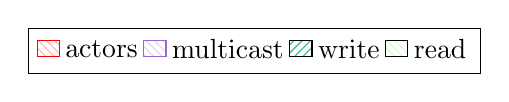
\begin{tikzpicture}
  \begin{axis}[ 
    xbar stacked,
    hide axis,
    xmin=0, xmax=1,
    ymin=0, ymax=1,
    legend style={at={(0,0)},anchor=north},
    legend columns=5,
    width=2cm,
    height=2cm
  ]
    \addlegendimage{red, pattern=north west lines, pattern color=candyapplered!30}
    \addlegendentry{actors}
    \addlegendimage{amethyst, pattern=north west lines, pattern color=amethyst!30}
    \addlegendentry{multicast}
    \addlegendimage{black, pattern=north east lines, pattern color=green(munsell)!80}
    \addlegendentry{write}
    \addlegendimage{black, pattern=north west lines, pattern color=green!20}
    \addlegendentry{read}
  \end{axis}
\end{tikzpicture}}
};
\end{scope}
}

%\newganttlinktype{newlink}{
%\ganttsetstartanchor{on right=1}
%\ganttsetendanchor{on left=0}
%\draw [ thick, cyan]
%(\xLeft, \yUpper) --
%(\xRight, \yLower);
%}

\newcommand{\gantChartUtilizationOnlyDRAM}
{
\begin{scope}

	\begin{ganttchart}[ bar height=0.5, vrule/.style={line width=0.5mm, black,loosely dashed}, canvas/.style={ draw=none},
                vrule label font=\bfseries, link/.style={->, line width=1pt, black}  ]{1}{44} 
                \ganttbar[bar left shift=0.1, bar right shift=-1,bar top shift=0.4,bar/.style={draw=none}]
                {\huge $\core_4$}{0}{44}
                \ganttActorbar[Actorbar top shift=0.0, inline,name=a4e1]{\Large $\actor_4$}{5}{10}
                \ganttActorbar[Actorbar top shift=0.0, inline]{\Large$\actor_4$}{29}{34}
                \\
                \ganttbar[bar left shift=0.1, bar right shift=-0.5,bar top shift=0.75,bar/.style={draw=none}]
                {\huge $\core_3$}{0}{30}
		\ganttActorbar[Actorbar top shift=0.4, inline,name=a3e1]{\Large$\actor_3$}{3}{8}
		\ganttActorbar[Actorbar top shift=0.4, inline]{\Large$\actor_3$}{27}{32}
		\\
                \ganttbar[bar left shift=0.1, bar right shift=-0.5,bar top shift=1.2,bar/.style={draw=none}]
                {\huge $\core_2$}{0}{30}
                \ganttBroadcastbar[Broadcastbar top shift=0.8,inline,name=a2e1]{\Large $\actor_2$ }{19}{20}        
                \ganttBroadcastbar[Broadcastbar top shift=0.8,inline]{\Large $\actor_2$ }{43}{44}        
                \\
                \ganttbar[bar left shift=0.1, bar right shift=-0.5,bar top shift=1.6,bar/.style={draw=none}]
                {\huge $\core_1$}{0}{30}
                \ganttActorbar[Actorbar top shift=1.25,inline,name=a1e1]{\Large $\actor_1$}{1}{4}   
                \ganttActorbar[Actorbar top shift=1.25,inline,name=a5e1]{\Large $\actor_5$}{17}{24}             

                \ganttActorbar[Actorbar top shift=1.25,inline]{\Large $\actor_1$}{25}{28}   
                \ganttActorbar[Actorbar top shift=1.25,inline]{\Large $\actor_5$}{41}{44}             

                \\
                \ganttbar[bar left shift=0.1, bar right shift=0.5,bar top shift=2, bar/.style={draw=none}]{\huge $\crossbar{1}$}{0}{38}
                \ganttCrossbarReadbar[CrossbarReadbar   top shift=1.7,inline,name=c2r1]{\Large $\channel_2$}{1}{2}
                \ganttCrossbarOpPrevbar[CrossbarOpPrevbar   top shift=1.7, inline]{\Large  $\channel_2$}{1}{2}
                \ganttCrossbarReadbar[CrossbarReadbar   top shift=1.7,inline,name=c3r1]{\Large  $\channel_3$}{3}{4}
                \ganttCrossbarOpPrevbar[CrossbarOpPrevbar   top shift=1.7, inline]{\Large  $\channel_3$}{3}{4}

                \ganttCrossbarWritebar[CrossbarWritebar top shift=1.7,inline,name=c1w1]{\Large $\channel_1$}{5}{6}             


                \ganttCrossbarWritebar[CrossbarWritebar top shift=1.7, inline,name=c4w1]{\Large $\channel_4$}{9}{10}             
                \ganttCrossbarWritebar[CrossbarWritebar top shift=1.7, inline,name=c5w1]{\Large $\channel_5$}{11}{12}            
                \ganttCrossbarReadbar[CrossbarReadbar   top shift=1.7,inline,name=c4r1]{\Large $\channel_4$}{13}{14}
                \ganttCrossbarReadbar[CrossbarReadbar   top shift=1.7,inline,name=c5r1]{\Large  $\channel_5$}{15}{16}

                \ganttCrossbarReadbar[CrossbarReadbar   top shift=1.7, inline,name=c1r1]{\Large  $\channel_1$}{17}{18}
                \ganttCrossbarWritebar[CrossbarWritebar top shift=1.7, inline,name=c2w1]{\Large $\channel_2$}{21}{22}             
                \ganttCrossbarWritebar[CrossbarWritebar top shift=1.7, inline,name=c3w1]{\Large $\channel_3$}{23}{24}            


                \ganttCrossbarReadbar [CrossbarReadbar  top shift=1.7,inline]{\Large $\channel_2$}{25}{26}
                \ganttCrossbarOpPrevbar[CrossbarOpPrevbar   top shift=1.7, inline]{\Large  $\channel_2$}{25}{26}
                \ganttCrossbarReadbar [CrossbarReadbar  top shift=1.7,inline]{\Large  $\channel_3$}{27}{28}
                \ganttCrossbarOpPrevbar[CrossbarOpPrevbar   top shift=1.7, inline]{\Large  $\channel_3$}{27}{28}
                \ganttCrossbarWritebar[CrossbarWritebar top shift=1.7,inline]{\Large $\channel_1$}{29}{30}             

                \ganttCrossbarWritebar[CrossbarWritebar top shift=1.7,inline]{\Large $\channel_4$}{33}{34}             
                \ganttCrossbarWritebar[CrossbarWritebar top shift=1.7,inline]{\Large $\channel_5$}{35}{36}            
                \ganttCrossbarReadbar [CrossbarReadbar  top shift=1.7,inline]{\Large $\channel_4$}{37}{38}
                \ganttCrossbarReadbar [CrossbarReadbar  top shift=1.7,inline]{\Large  $\channel_5$}{39}{40}
                \ganttCrossbarReadbar [CrossbarReadbar  top shift=1.7,inline]{\Large  $\channel_1$}{41}{42}
		
		\\

		\ganttbar[bar/.style={draw=none}]{\huge }{0}{38}
       		\\
		\ganttbar[bar/.style={draw=none}]{\huge }{0}{38}      

        \draw[-Latex,line width=0.3mm,opacity=0.75] (c2r1) |- (a3e1);
        \draw[-Latex,line width=0.3mm,opacity=0.75] (c3r1) |- (a4e1);
        \draw[-Latex,line width=0.3mm,opacity=0.75] (a1e1) -| (c1w1);
        \draw[-Latex,line width=0.3mm,opacity=0.75] (a3e1) -| (c4w1);
        \draw[-Latex,line width=0.3mm,opacity=0.75] (a4e1) -| (c5w1);
        \draw[-Latex,line width=0.3mm,opacity=0.75] (c4r1) |- (a5e1);
        \draw[-Latex,line width=0.3mm,opacity=0.75] (c5r1.north) -- (a5e1.west);

        \draw[-Latex,line width=0.3mm,opacity=0.75] (c1r1) |- (a2e1);
        \draw[-Latex,line width=0.3mm,opacity=0.75] (a2e1) -| (c2w1);
        \draw[-Latex,line width=0.3mm,opacity=0.75] (a2e1) -| (c3w1);

        \draw[-{Stealth},line width=0.3mm] (0,-7) -- (23.5,-7);
        \draw[-{Stealth},line width=0.3mm] (0,-7) -- (0,1);

	\ganttvrule{\Large}{0}
	\ganttvrule{\Large}{24}
	%\ganttvrule{\Large}{44}

	 \foreach \x in {0,...,22}{
 		{\pgfmathtruncatemacro{\label}{(\x)}
		\node at (\x,-7.4) {\Large \label};}
		\draw[line width=0.4mm](\x,-6.8) -- (\x,-7.2);
	}

	\draw[line width=0.4mm](-0.15,-6.25) -- (0.2,-6.25);
	\draw[line width=0.4mm](-0.15,-4.8) -- (0.2,-4.8);
	\draw[line width=0.4mm](-0.15,-3.45) -- (0.2,-3.45);
	\draw[line width=0.4mm](-0.15,-2) -- (0.2,-2);
	\draw[line width=0.4mm](-0.15,-0.65) -- (0.2,-0.65);
	\node at (23,0.5) {\Large $\Period=12$};
	\node at (23,-6.5) {\Large Time};

\draw [line width=0.25mm,color=black,decorate,decoration={brace,amplitude=10pt,raise=4pt},yshift=0pt] (0,0) -- (12,0) node [black,midway,xshift=0cm,yshift=1cm] { \Large $n$ };

    \end{ganttchart} 

\end{scope} 
}


\newcommand{\gantChartUtilizationNoReads}
{
\begin{scope}

	\begin{ganttchart}[ bar height=0.5, vrule/.style={line width=0.5mm, black,loosely dashed}, canvas/.style={ draw=none},
                vrule label font=\bfseries, link/.style={->, line width=1pt, black}  ]{1}{44} 

		\ganttbar[bar left shift=0.1, bar right shift=-1,bar top shift=0.4,bar/.style={draw=none}]
                {\huge $\core_4$}{0}{30}
		\ganttActorbar[Actorbar top shift=0.0, inline,name=a4e1]{\Large $\actor_4$}{1}{6}
		\ganttActorbar[Actorbar top shift=0.0, inline]{\Large $\actor_4$}{19}{24}
		\ganttActorbar[Actorbar top shift=0.0, inline]{\Large $\actor_4$}{37}{42}
                \\
		\ganttbar[bar left shift=0.1, bar right shift=-0.5,bar top shift=0.75,bar/.style={draw=none}]
                {\huge $\core_3$}{0}{30}
		\ganttActorbar[Actorbar top shift=0.4, inline,name=a3e1]{\Large$\actor_3$}{1}{6}
		\ganttActorbar[Actorbar top shift=0.4, inline]{\Large$\actor_3$}{19}{24}
		\ganttActorbar[Actorbar top shift=0.4, inline]{\Large$\actor_3$}{37}{42}

		\\
		\ganttbar[bar left shift=0.1, bar right shift=-0.5,bar top shift=1.2,bar/.style={draw=none}]
                {\huge $\core_2$}{0}{30}
                \ganttBroadcastbar[Broadcastbar top shift=0.8,inline,name=a2e1]{\Large $\actor_2$}{7}{8}        
                \ganttBroadcastbar[Broadcastbar top shift=0.8,inline]{\Large $\actor_2$ }{25}{26}        
                \ganttBroadcastbar[Broadcastbar top shift=0.8,inline]{\Large $\actor_2$ }{43}{44}        

                \\
		\ganttbar[bar left shift=0.1, bar right shift=-0.5,bar top shift=1.6,bar/.style={draw=none}]
                {\huge $\core_1$}{0}{30}
		\ganttActorbar[Actorbar top shift=1.25,inline,name=a1e1]{\Large $\actor_1$}{1}{4} 
                \ganttActorbar[Actorbar top shift=1.25,inline,name=a5e1]{\Large $\actor_5$}{11}{18}             

		\ganttActorbar[Actorbar top shift=1.25,inline]{\Large $\actor_1$}{19}{22} 
                \ganttActorbar[Actorbar top shift=1.25,inline]{\Large $\actor_5$}{29}{36}             

		\ganttActorbar[Actorbar top shift=1.25,inline]{\Large $\actor_1$}{37}{40} 

 
                \\
		\ganttbar[bar left shift=0.1, bar right shift=0.5,bar top shift=2, bar/.style={draw=none}]{\huge $\crossbar{1}$}{0}{38}
		\ganttCrossbarWritebar[CrossbarWritebar top shift=1.7,inline,name=c1w1]{\Large $\channel_1$}{5}{6}
                \ganttCrossbarWritebar[CrossbarWritebar top shift=1.7, inline,name=c4w1]{\Large $\channel_4$}{7}{8}             
                \ganttCrossbarWritebar[CrossbarWritebar top shift=1.7, inline,name=c5w1]{\Large $\channel_5$}{9}{10}            

                \ganttCrossbarWritebar[CrossbarWritebar top shift=1.7, inline,name=c2w1]{\Large $\channel_2$}{11}{12}             
                \ganttCrossbarWritebar[CrossbarWritebar top shift=1.7, inline,name=c3w1]{\Large $\channel_3$}{13}{14}            

		\ganttCrossbarWritebar[CrossbarWritebar top shift=1.7,inline ]{\Large $\channel_1$}{23}{24}
                \ganttCrossbarWritebar[CrossbarWritebar top shift=1.7, inline]{\Large $\channel_4$}{25}{26}             
                \ganttCrossbarWritebar[CrossbarWritebar top shift=1.7, inline]{\Large $\channel_5$}{27}{28}            

                \ganttCrossbarWritebar[CrossbarWritebar top shift=1.7, inline]{\Large $\channel_2$}{29}{30}             
                \ganttCrossbarWritebar[CrossbarWritebar top shift=1.7, inline]{\Large $\channel_3$}{31}{32}            

		\ganttCrossbarWritebar[CrossbarWritebar top shift=1.7,inline ]{\Large $\channel_1$}{41}{42}
                \ganttCrossbarWritebar[CrossbarWritebar top shift=1.7, inline]{\Large $\channel_4$}{43}{44}             
%                \ganttCrossbarWritebar[CrossbarWritebar top shift=1.7, inline]{\Large $\channel_5$}{43}{44}            

		\\
		\ganttbar[bar/.style={draw=none}]{\huge }{0}{38}
       		\\
		\ganttbar[bar/.style={draw=none}]{\huge }{0}{38}      

        \draw[-Latex,line width=0.3mm,opacity=0.75] (a1e1) -| (c1w1);
	\draw[-Latex,line width=0.3mm,opacity=0.75] (a3e1) -- (c4w1);  
	\draw[-Latex,line width=0.3mm,opacity=0.75] (a4e1) -| (c5w1); 
	\draw[-Latex,line width=0.3mm,opacity=0.75] (a2e1) -- (c2w1);
	\draw[-Latex,line width=0.3mm,opacity=0.75] (a2e1) -- (c3w1);

	\ganttvrule{\Large}{0}
	\ganttvrule{\Large}{18}
	\ganttvrule{\Large}{36}

        \draw[-{Stealth},line width=0.3mm] (0,-7) -- (23.5,-7);
        \draw[-{Stealth},line width=0.3mm] (0,-7) -- (0,1);

	 \foreach \x in {0,...,22}{
 		{\pgfmathtruncatemacro{\label}{(\x)}
		\node at (\x,-7.4) {\Large \label};}
		\draw[line width=0.4mm](\x,-6.8) -- (\x,-7.2);
	}

	\draw[line width=0.4mm](-0.15,-6.25) -- (0.2,-6.25);
	\draw[line width=0.4mm](-0.15,-4.8) -- (0.2,-4.8);
	\draw[line width=0.4mm](-0.15,-3.45) -- (0.2,-3.45);
	\draw[line width=0.4mm](-0.15,-2) -- (0.2,-2);
	\draw[line width=0.4mm](-0.15,-0.65) -- (0.2,-0.65);
	\node at (23,0.5) {\Large $\Period=9$};
	\node at (23,-6.5) {\Large Time};

\draw [line width=0.25mm,color=black,decorate,decoration={brace,amplitude=10pt,raise=4pt},yshift=0pt] (0,0) -- (9,0) node [black,midway,xshift=0cm,yshift=1cm] { \Large $n$ };
\draw [line width=0.25mm,color=black,decorate,decoration={brace,amplitude=10pt,raise=4pt},yshift=0pt] (9,0) --(18,0) node [black,midway,xshift=0cm,yshift=1cm] { \Large $n+1$ };
        \end{ganttchart} 

\end{scope} 
}


\newcommand{\legendArch}
{
\pgfplotsset{ytick style={draw=none}}
%  \begin{scope}
        \begin{axis}[
                xbar stacked,
                hide axis,
                xmin=0,
                xmax=1,
                width=2cm,
                height=2cm,
                ymin=0,
                ymax=0.4,
                legend style={at={(0.5,-0.4)},anchor=north},
                legend columns=5,
                ]
                        \addlegendimage{black,fill=bananayellow!25}
                        \addlegendentry{Tile $\tile_1$}
                        \addlegendimage{black, fill=bleudefrance!25}
                        \addlegendentry{Tile $\tile_2$}
                        \addlegendimage{black, fill=brickred!25}
                        \addlegendentry{Tile $\tile_3$}
                        \addlegendimage{black, fill=emerald!70}
                        \addlegendentry{Local memory ($\SetMemoriesLocal$)}
                        \addlegendimage{black, fill=amethyst!60}
                        \addlegendentry{Tile local memory ($\SetTileLocalMemories$)}
        \end{axis}
%    \end{scope}
}

\newcommand{\legendApp}
{
\pgfplotsset{ytick style={draw=none}}
%  \begin{scope}
        \begin{axis}[
                xbar stacked,
                hide axis,
                xmin=0,
                xmax=1,
                width=2cm,
                height=2cm,
                ymin=0,
                ymax=0.4,
                legend style={at={(0.5,-0.4)},anchor=north},
                legend columns=3,
                ]
                        \addlegendimage{black,fill=candyapplered!30}
                        \addlegendentry{actors}
                        \addlegendimage{black, fill=amethyst!30}
                        \addlegendentry{multicast actor}
                        \addlegendimage{black, fill=green(munsell)!30}
                        \addlegendentry{channels}
        \end{axis}
%    \end{scope}
}

\newcommand{\simpleApplication}[2]{
  \def \xshift{#1}
  \def \yshift{#2}
  \node[ActorStyle] (actorSource)           at (-0.25+\xshift,0+\yshift) {\Large $a_1$};
  \node[ChannelStyle] (channelZero)         at (1.5+\xshift,0+\yshift) {\Large $c_1$};
  \node[ActorBroadcastStyle] (broadCastOne) at (3.25+\xshift,0+\yshift) {\Large $a_2$};
  \node[ChannelStyle] (channelOne)          at (4.75+\xshift,1.25+\yshift) {\Large $c_2$};
  \node[ChannelStyle] (channelTwo)          at (4.75+\xshift,-1.25+\yshift) {\Large $c_3$};
  \node[ActorStyle] (vertical)              at (6.25+\xshift,2+\yshift) {\Large $a_3$};
  \node[ActorStyle] (horizontal)            at (6.25+\xshift,-2+\yshift) {\Large $a_4$ };
  \node[ChannelStyle] (channelThree)        at (7.75+\xshift,1.25+\yshift) {\Large $c_4$};
  \node[ChannelStyle] (channelFour)         at (7.75+\xshift,-1.25+\yshift) {\Large $c_5$};
  \node[ActorStyle] (sink)                  at (9+\xshift,0+\yshift) {\Large $a_5$ };
%  % now draw the arrows
  
 \draw[ArrowStyle] (actorSource) -- (channelZero);
  \draw[ArrowStyle] (channelZero) -- (broadCastOne);
  
  \draw[ArrowStyle] (broadCastOne) -- (channelOne);
  \draw[ArrowStyle] (broadCastOne) -- (channelTwo);
  \draw[ArrowStyle] (channelOne) -- (vertical);
  \draw[ArrowStyle] (channelTwo)  -- (horizontal);
  
  \draw[ArrowStyle] (vertical)  -- (channelThree);
  \draw[ArrowStyle] (horizontal)  -- (channelFour);
  \draw[ArrowStyle] (channelThree) --  (sink);
  \draw[ArrowStyle] (channelFour)  -- (sink);
}

\newcommand{\TileTemplate}[5]{
        \draw[draw=black,fill=#1!25,line width=0.15mm] (-0.5,-0.25) rectangle (5.0,3.8);
        
        \node[rectangle,draw,line width=0.15mm,fill=#1,minimum width=1cm] (CPU1) at (1,3.25) {\large $\core_{#3}$};
        \node at (2.25,2.9) {\Huge $\ldots$};
        \node[rectangle,draw,line width=0.15mm,fill=#1,minimum width=1cm] (CPU#2) at (3.5,3.25) {\large $\core_{#2}$};
        \node[rectangle,draw,line width=0.15mm,fill=emerald!70,minimum width=1cm] (lmem1) at (1,2.25) {\large $\memory_{#3}$};
        \node[rectangle,draw,line width=0.15mm,fill=emerald!70,minimum width=1cm] (lmem#2) at (3.5,2.25) {\large $\memory_{#2}$};
        
        \node[rectangle,draw,line width=0.2mm,minimum width=4cm,fill=internationalorange!50] (crossbar) at (2.25,1.25) {\large $\crossbar_{#4}$};
        
        \node[rectangle,draw,line width=0.2mm,minimum width=4cm,fill=amethyst!60] (tileMem) at (2.25,0.25) {\large $\memory_{#5}$};
        
        \draw[<->,>=triangle 60,] (CPU1) -- (lmem1);
        \draw[<->,>=triangle 60,] (CPU#2) -- (lmem#2);

        \draw[<->,>=triangle 60,] (lmem1) -- ($(lmem1.south)+(0,-0.45)$);
        \draw[<->,>=triangle 60,] (lmem#2) -- ($(lmem#2.south)+(0,-0.45)$);
        
        \draw[<->,>=triangle 60,] (CPU1.west) -- ($(CPU1.west)+(-0.75,0)$) |- (crossbar);
        \draw[<->,>=triangle 60,] (CPU#2.east) -- ($(CPU#2.east)+(0.75,0)$) |- (crossbar);
        
        \draw[<->,>=triangle 60,] (crossbar) -- (tileMem);
}

\newcommand{\architectureMultiTile}{
    \simpleApplication{-18.5}{-1.2}

    \node (tileA) at (-6,-0.2){
    \begin{tikzpicture}
        \TileTemplate{bananayellow}{4}{1}{1}{21}
    \end{tikzpicture}};

    \node (tileB) at (0,-0.2){
    \begin{tikzpicture}
        \TileTemplate{bleudefrance}{12}{5}{2}{22}
    \end{tikzpicture}};
    
    \node (tileC) at (6,-0.2){
    \begin{tikzpicture}
        \TileTemplate{brickred}{20}{13}{3}{23}
    \end{tikzpicture}};
  
    \node[rectangle,draw,line width=0.2mm,minimum width=17.75cm,fill=amber] (noc) at (0.1,-3.15) {$\NoC$};
    \node[rectangle,draw,line width=0.2mm,minimum width=17.75cm,fill=electricgreen!50] (globalMem) at (0.1,-4.2) {$\GlobalMemory$};
    
    \draw[<->,>=triangle 60,] ($(tileA.south)+(0,0.1)$) -- ($(tileA.south)+(0,-0.5)$);
    \draw[<->,>=triangle 60,] ($(tileB.south)+(0,0.1)$) -- ($(tileB.south)+(0,-0.5)$);
    \draw[<->,>=triangle 60,] ($(tileC.south)+(0,0.1)$) -- ($(tileC.south)+(0,-0.53)$);
    \draw[<->,>=triangle 60,] (noc) -- (globalMem);

    \node at (0,-5){
      \resizebox{380pt}{!}{  
      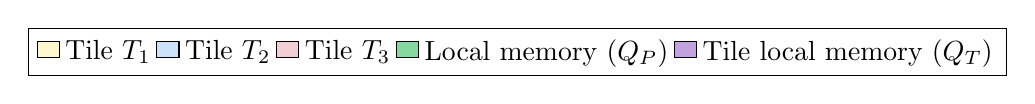
\begin{tikzpicture}
        \legendArch
      \end{tikzpicture}}
    };

    \node at (-14,-5){
      \resizebox{200pt}{!}{  
      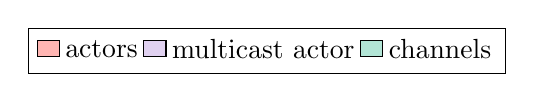
\begin{tikzpicture}
        \legendApp
      \end{tikzpicture}}
    };
    % draw mappings
    \node(tile1) at (-8,1.5) {};
    \node(tile2) at (-2.3,1.5) {};
    \node(tile3) at (3.5,-1.65) {};

    \draw[MappingStyle,line width=0.5mm,draw=red] (sink)  -- (tile1);
    \draw[MappingStyle,line width=0.5mm,draw=red] (sink)  -- (tile2);
    \draw[MappingStyle,line width=0.5mm,draw=red] (sink)  -- (tile3);

    \node(global) at (-1.25,-4.0) {};
    \node(local1) at (-7.35,0.3) {};
    \node(local2) at (-5.0,0.2) {};
    \node(local3) at (-1.5,0.4) {};
    \node(local4) at (1.25,0.0) {};
    \node(local5) at (5,0.3) {};
    \node(local6) at (7.5,0.3) {};
    \node(tileLocal1) at (-4.0,-1.5) {};
    \node(tileLocal2) at (-1.8,-1.65) {};
    \node(tileLocal3) at (4.0,-1.5) {};

    \draw[MappingStyle,line width=0.5mm,draw=blue] (channelFour)  -- (local3);
    \draw[MappingStyle,line width=0.5mm,draw=blue] (channelFour)  -- (local4);
    \draw[MappingStyle,line width=0.5mm,draw=blue] (channelFour)  -- (tileLocal2);
    \draw[MappingStyle,line width=0.5mm,draw=blue] (channelFour)  -- (global);

}


\newcommand{\FIFODrawing}{
	\draw[draw=black,fill=white] (0.0,0) rectangle (1.5,0.75);
	\draw[draw=black] (0.75,0) -- (0.75,0.75);
	
	\node[mark size=1.4mm] at (0.38,0.35) {\pgfuseplotmark{*}};

	\fill [black!40,opacity=0.1] (0,0) -- (0,0.75) -- (-1.5,-0.25);
	\draw [black,densely dotted] (0,0) -- (0,0.75) -- (-1.5,-0.25) -- (0,0);
	
}

\newcommand{\FIFODrawingTwo}{
	\draw[draw=black,fill=white] (0,0) rectangle (1.5,0.75);
	\draw[draw=black] (0.75,0) -- (0.75,0.75);
	
	\node[mark size=1.4mm] at (0.38,0.35) {\pgfuseplotmark{*}};

	\fill [black!40,opacity=0.1] (0,0) -- (0,0.75) -- (-1.5,0.6);
	\draw [black,densely dotted] (0,0) -- (0,0.75) -- (-1.5,0.6) -- (0,0);
	
}

\newcommand{\FIFODrawingFour}{
	\draw[draw=black,fill=white] (1,0) rectangle (4,0.75);
        \draw[draw=black] (1.75,0)   -- (1.75,0.75);
        \draw[draw=black] (2.5,0) -- (2.5,0.75);
        \draw[draw=black] (3.25,0) -- (3.25,0.75);
	
	\node[mark size=1.4mm] at (1.38,0.35) {\pgfuseplotmark{*}};

        \fill [black!40,opacity=0.1] (-0.25,0.35) -- (1.0,0.75) -- (1.0,0.0);
        \draw [black,densely dotted] (-0.25,0.35) -- (1.0,0.75) -- (1.0,0.0) -- (-0.25,0.35);

}

\newcommand{\FIFODrawingThree}{
	\draw[draw=black,fill=white] (0,0) rectangle (1.5,0.75);
	\draw[draw=black] (0.75,0) -- (0.75,0.75);

	\fill [black!40,opacity=0.1] (0,0) -- (1.5,0) -- (1,-1.5);
	\draw [black,densely dotted] (0,0) -- (1.5,0) -- (1,-1.5) -- (0,0);
	
}

\newcommand{\memoryDDR}{
 \draw[fill=electricgreen!50] (0,0) rectangle (1,-7);
 \draw[line width=0.44mm] (0,-2) -- (1,-2);
 \draw[line width=0.15mm] (0,-1) -- (1,-1);
 \draw[line width=0.44mm] (0,-4) -- (1,-4);
 \draw[line width=0.15mm] (0,-3) -- (1,-3);
 \draw[line width=0.44mm] (0,-6) -- (1,-6);
 \draw[line width=0.15mm] (0,-5) -- (1,-5);

 \node[mark size=1.4mm] at (0.5,-2.5) {\pgfuseplotmark{*}};
 \node[mark size=1.4mm] at (0.5,-4.5) {\pgfuseplotmark{*}};

 \node at (0.5,-6.5) {\Huge \ldots};
}


\newcommand{\memoryDDRPointer}{
 \draw[fill=electricgreen!50] (0,0) rectangle (1,-7);
 \draw[line width=0.44mm] (0,-2) -- (1,-2);
 \draw[line width=0.15mm] (0,-1) -- (1,-1);
 \draw[line width=0.44mm] (0,-4) -- (1,-4);
 \draw[line width=0.15mm] (0,-3) -- (1,-3);

 \node[mark size=1.4mm] at (0.5,-0.5) {\pgfuseplotmark{*}};
 \node at (0.5,-6.5) {\Huge \ldots};
}

\newcommand{\FIFOMapping}{
\node  (fifoThree) at (1.5,0.9) {
		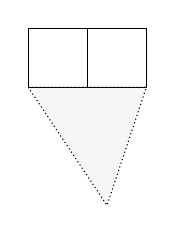
\begin{tikzpicture}
			\FIFODrawingThree
		\end{tikzpicture}
	};

\node (leg) at (1.5,-1.4) {\large \begin{tabular}{ll}$\Size(c)$&$=38$\,kB\\ $\Capacity(c)$&$=2$  \end{tabular}};
\node[ActorStyle] (convert) at (0,0) {\large $a_1$};
\node[ChannelStyle] (channelTwo) at (1.5,0) {\large $c_1$};
\node[ActorBroadcastStyle] (broadCastOne) at (3,0) {\large $a_2$};
\node[ChannelStyle] (channelThree) at (4.5,1.25) {\large $c_2$};
\node[ChannelStyle] (channelFour)  at (4.5,-1.25) {\large $c_3$};
\node[ActorStyle] (vertical) at (6,2) {\large $a_3$};
\node[ActorStyle] (horizontal) at (6,-2) {\large $a_4$ };

% now draw the arrows
\draw[ArrowStyle] (convert) -- (channelTwo);
\draw[ArrowStyle] (channelTwo) -- (broadCastOne);
\draw[ArrowStyle] (broadCastOne) -- (channelThree);
\draw[ArrowStyle] (broadCastOne) -- (channelFour);
\draw[ArrowStyle] (channelThree) -- (vertical);
\draw[ArrowStyle] (channelFour)  -- (horizontal);

%\draw [draw=black] (6,-3) rectangle (8,3);
\begin{scope}
\node[ChannelStyle] (channelFive) at (7.5,1.25) {\large $c_4$};
\node[ChannelStyle] (channelSix)  at (7.5,-1.25){\large $c_5$};

\draw[ArrowStyle] (vertical) -- (channelFive);
\draw[ArrowStyle] (horizontal) -- (channelSix);

\path [scope fading=west] (6.5,-3) rectangle (8,3);
\fill [fill=white] (6.5,-3) rectangle (8,3);

\end{scope}

\node  (fifoOne) at (6.0,-0.8) {
		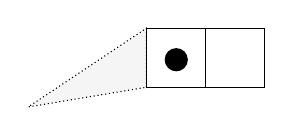
\begin{tikzpicture}
			\FIFODrawing
		\end{tikzpicture}
	};

\node  (fifoTwo) at (6.0,0.8) {
		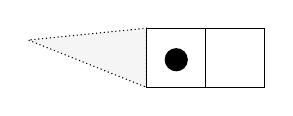
\begin{tikzpicture}
			\FIFODrawingTwo
		\end{tikzpicture}
	};


\node  (memDDR) at (10,0.5) {
		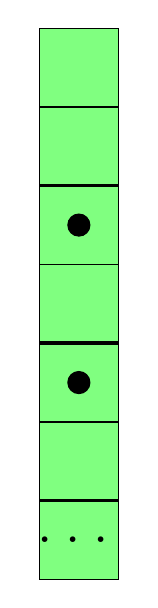
\begin{tikzpicture}
			\memoryDDR
		\end{tikzpicture}
	};

\node (legendStatic) at (4.5,-3.5){
                \resizebox{200pt}{!}{
                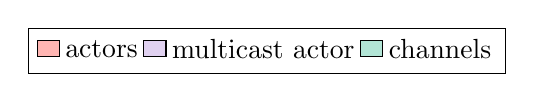
\begin{tikzpicture}
                        \legendApp
                \end{tikzpicture}}
        };

\node (legChannel1) at (8.75,3) {};
\node (legChannel2) at (8.75,1) {};
\node (legChannel3) at (8.75,-1){};

\draw [decorate,decoration={brace,amplitude=10pt,mirror,raise=4pt},yshift=0pt] (9.6,4) -- (9.6,2) node  [black,midway,xshift=0cm,yshift=-1cm] {};
\draw [decorate,decoration={brace,amplitude=10pt,mirror,raise=4pt},yshift=0pt] (9.6,2) -- (9.6,0) node  [black,midway,xshift=0cm,yshift=-1cm] {};
\draw [decorate,decoration={brace,amplitude=10pt,mirror,raise=4pt},yshift=0pt] (9.6,0) -- (9.6,-2) node [black,midway,xshift=0cm,yshift=-1cm] {};

\draw[->, >=triangle 60,dashed] (fifoOne.east) -- (legChannel3);
\draw[->, >=triangle 60,dashed] (fifoTwo.east) -- (legChannel2);
\draw (fifoThree.north) edge[bend  left=20,->,>= triangle 60,dashed] (legChannel1);
\node (leg) at (10,-3.5) {\Large \begin{tabular}{c}global memory \\ ($\GlobalMemory$) \end{tabular}};

\node[ChannelStyle]  at (4.5,1.25) {\large $c_2$};
\node[ChannelStyle]  at (4.5,-1.25) {\large $c_3$};
}


\newcommand{\FIFOPointerBasedMapping}{

%\draw[fill=green(munsell)!30,opacity=0.5,line width=0.25mm] (1.1,1.7) rectangle (4.9,-1.7);
%\draw[draw=black,line width=0.25mm] (1.1,1.7) rectangle (4.9,-1.7);
\draw[fill=green(munsell)!30,opacity=0.5,line width=0.25mm,radius=63pt] (3.3,0) circle;
\draw[draw=black,line width=0.25mm,radius=63pt] (3.3,0) circle;

\node (leg) at (0,-3) {\Large \begin{tabular}{ll} $\Size(c_{\{1,2,3\}})$ & $=38$\,kB\\ $\Capacity(c_{\{1,2,3\}})$ & $=4$ \end{tabular}};

%\node (leg) at (2.75,2.75) {\Large \color{black}{capacity($c_{\{1,2,3\}}$)$=8$}};
\node (leg) at (3.0,-1.5) {\huge \color{black}{$c_{\{1,2,3\}}$}};
%\begin{scope}[path fading]
\node[ActorStyle] (convert) at (0,0) {\Large $a_1$};
\node[ChannelStyle,opacity=0.3,text opacity=1] (channelTwo) at (1.5,0) {\large $c_1$};
\node[ActorBroadcastStyle,opacity=0.5,text opacity=1] (broadCastOne) at (3,0) {\large $a_2$};
\node[ChannelStyle,opacity=0.3,text opacity=1] (channelThree) at (4.5,1.25) {\Large $c_2$};
\node[ChannelStyle,opacity=0.3,text opacity=1] (channelFour)  at (4.5,-1.25) {\Large $c_3$};
\node[ActorStyle] (vertical) at (6,2) {\Large $a_3$};
\node[ActorStyle] (horizontal) at (6,-2) {\Large $a_4$ };
% now draw the arrows
\draw[ArrowStyle] (convert) -- (channelTwo);
\draw[ArrowStyle] (channelTwo) -- (broadCastOne);
\draw[ArrowStyle] (broadCastOne) -- (channelThree);
\draw[ArrowStyle] (broadCastOne) -- (channelFour);
\draw[ArrowStyle] ($(channelThree)+(0.5,0)$) -- (vertical);
\draw[ArrowStyle] ($(channelFour)+(0.5,0)$)  -- (horizontal);
\begin{scope}
\node[ChannelStyle] (channelFive) at (7.5,1.25) {\large $c_4$};
\node[ChannelStyle] (channelSix)  at (7.5,-1.25) {\large $c_5$};
\draw[ArrowStyle] (vertical) -- (channelFive);
\draw[ArrowStyle] (horizontal) -- (channelSix);
\path [scope fading=west] (6.5,-3) rectangle (8,3);
\fill [fill=white] (6.5,-3) rectangle (8,3);
\end{scope}

\node  (fifoTwo) at (7.5,-0.1) {
		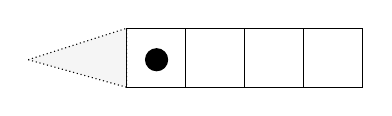
\begin{tikzpicture}
			\FIFODrawingFour
		\end{tikzpicture}
	};
%\draw[->, >=triangle 60,dashed] ($(channelThree)+(0,-1.5)$) -- (fifoTwo);
%\draw[->, >=triangle 60,dashed] ($(channelFour)+(0.1,0.6)$) -- ($(fifoTwo)+(0,0.2)$);
%\end{scope}
\node  (memDDR) at (10.5,0.5) {
		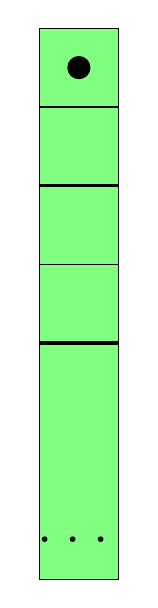
\begin{tikzpicture}
			\memoryDDRPointer
		\end{tikzpicture}
	};

    \node (legendStatic) at (5,-3.5){
                \resizebox{200pt}{!}{
                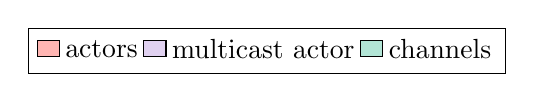
\begin{tikzpicture}
                        \legendApp
                \end{tikzpicture}}
        };

\draw [decorate,decoration={brace,amplitude=10pt,mirror,raise=4pt},yshift=0pt] (10.2,4) -- (10.2,0) node  [black,midway,xshift=0cm,yshift=-1cm] {};
\node (legChannel1) at (9.5,2) {};
\node(MRBleg) at ($(fifoTwo.north)+(0.3,0.2)$) {\Large $\channel_{\{1,2,3\}}$'s buffer};
\draw[->, >=triangle 60,dashed] ($(MRBleg.north)+(0.8,0)$) -- (legChannel1);
\node (leg) at (10.5,-3.5) {\Large \begin{tabular}{c}global memory \\ ($\GlobalMemory$) \end{tabular}};



}








\newcommand{\writingFIFOEmpty}{
        \draw[draw=black,fill=white] (2,0) rectangle (5.6,0.75);
        \draw[draw=black] (2.9,0)   -- (2.9,0.75);
        \draw[draw=black] (3.8,0) -- (3.8,0.75);
        \draw[draw=black] (4.7,0) -- (4.7,0.75);

        \node[mark size=1.4mm,color=white] (t4) at (5.15,0.35) {\pgfuseplotmark{*}};
        \node[mark size=1.4mm,color=white] (t3) at (4.25,0.35) {\pgfuseplotmark{*}};
        \node[mark size=1.4mm,color=white] (t2) at (3.35,0.35) {\pgfuseplotmark{*}};
        \node[mark size=1.4mm,color=white] (t1) at (2.45,0.35) {\pgfuseplotmark{*}};
        
        \node[ActorStyle] (actor1) at (0.0,0.35)  {\huge $a_{1}$};
        \node[ActorStyle] (actor2) at (6.75,1)    {\huge $a_{3}$};
        \node[ActorStyle] (actor3) at (6.75,-0.7) {\huge $a_{4}$};
        
        \draw[->,>=triangle 60,densely dotted,line width=0.3mm] (actor1.north) -- ($(actor1.north)+(0,0.35)$) -| ($(t1)+(-0.2,0.4)$);
%        \draw[<-,>=triangle 60,dashed,line width=0.3mm] (actor2.north) -- ($(actor2.north)+(0,0.4)$) -| ($(t1)+(0.2,0.4)$);
%        \draw[<-,>=triangle 60,dashed,line width=0.3mm] (actor3.south) -- ($(actor3.south)+(0,-0.4)$) -| ($(t1)+(0,-0.4)$);
        
        \node at ($(actor1.south)+(0,-0.3)$) {\Large writer};
        \node at ($(actor3.south)+(0,-0.6)$) {\Large readers};
        
%        \node[]  at (3.25,-0.25) {\Large $\SetTokens_1=\{\ \ \ 0,\ \ \ 0,\ \ \ 0,\ \ \ 0\ \ \ \}$};
%        \node[]  at (3.25,-0.75) {\Large $\SetTokens_2=\{\ \ \ 0,\ \ \ 0,\ \ \ 0,\ \ \ 0\ \ \ \}$};

        \node at (0.4,1.6)  {\Large $\Write_{\channel_{\{1,2,3\}}}=0$};
        \node at (4.2,1.6)  {\Large $\Read_{\channel_{\{1,2,3\}},\actor_3}=-1$};
        \node at (4.2,-1.3) {\Large $\Read_{\channel_{\{1,2,3\}},\actor_4}=-1$};

%        \node at (0.5,-1.4) {\Large $\mathsf{T}(a_{src}) = 0$};
%        \node at (0.5,-1.95) {\Large $\mathsf{T}(a_{(dst,1)}) = 0$};
%        \node at (0.5,-2.5) {\Large $\mathsf{T}(a_{(dst,2)}) = 0$};
}

\newcommand{\writingFIFO}{
        \draw[draw=black,fill=white] (2,0) rectangle (5.6,0.75);
        \draw[draw=black] (2.9,0)   -- (2.9,0.75);
        \draw[draw=black] (3.8,0) -- (3.8,0.75);
        \draw[draw=black] (4.7,0) -- (4.7,0.75);

        \node[mark size=1.4mm,color=white] (t4) at (5.15,0.35) {\pgfuseplotmark{*}};
        \node[mark size=1.4mm] (t3) at (4.25,0.35) {\pgfuseplotmark{*}};
        \node[mark size=1.4mm] (t2) at (3.35,0.35) {\pgfuseplotmark{*}};
        \node[mark size=1.4mm] (t1) at (2.45,0.35) {\pgfuseplotmark{*}};
        
        \node[ActorStyle] (actor1) at (0.0,0.35)  {\huge $a_{1}$};
        \node[ActorStyle] (actor2) at (6.75,1)     {\huge $a_{3}$};
        \node[ActorStyle] (actor3) at (6.75,-0.7) {\huge $a_{4}$};
        
        \draw[->,>=triangle 60,densely dotted,line width=0.3mm] (actor1.north) -- ($(actor1.north)+(0,0.35)$) -| ($(t4)+(0,0.4)$);
        \draw[<-,>=triangle 60,dashed,line width=0.3mm] (actor2.north) -- ($(actor2.north)+(0,0.4)$) -| ($(t1)+(0,0.4)$);
        \draw[<-,>=triangle 60,dashed,line width=0.3mm] (actor3.south) -- ($(actor3.south)+(0,-0.4)$) -| ($(t1)+(0,-0.4)$);
        
        \node at ($(actor1.south)+(0,-0.3)$) {\Large writer};
        \node at ($(actor3.south)+(0,-0.6)$) {\Large readers};
        
%        \node[]  at (3.25,-0.25) {\Large $\SetTokens_1=\{\ \ \ 1,\ \ \ 1,\ \ \ 1,\ \ \ 0\ \ \ \}$};
%        \node[]  at (3.25,-0.75) {\Large $\SetTokens_2=\{\ \ \ 1,\ \ \ 1,\ \ \ 1,\ \ \ 0\ \ \ \}$};


        \node at (0.4,1.6)  {\Large $\Write_{\channel_{\{1,2,3\}}}=3$};
        \node at (4.4,1.6)  {\Large $\Read_{\channel_{\{1,2,3\}},\actor_3}=0$};
        \node at (4.2,-1.3) {\Large $\Read_{\channel_{\{1,2,3\}},\actor_4}=0$};

%        \node at (0.5,-1.4) {\Large $\mathsf{T}(a_{src}) = 3$};
%        \node at (0.5,-1.95) {\Large $\mathsf{T}(a_{(dst,1)}) = 3$};
%        \node at (0.5,-2.5) {\Large $\mathsf{T}(a_{(dst,2)}) = 3$};
}

\newcommand{\writingFIFOSecond}{
        \draw[draw=black,fill=white] (2,0) rectangle (5.6,0.75);
        \draw[draw=black] (2.9,0)   -- (2.9,0.75);
        \draw[draw=black] (3.8,0) -- (3.8,0.75);
        \draw[draw=black] (4.7,0) -- (4.7,0.75);

        \node[mark size=1.4mm] (t4) at (5.15,0.35) {\pgfuseplotmark{*}};
        \node[mark size=1.4mm] (t3) at (4.25,0.35) {\pgfuseplotmark{*}};
        \node[mark size=1.4mm] (t2) at (3.35,0.35) {\pgfuseplotmark{*}};
        \node[mark size=1.4mm] (t1) at (2.45,0.35) {\pgfuseplotmark{*}};

        \node[ActorStyle] (actor1) at (0.0,0.35)  {\huge $a_{1}$};
        \node[ActorStyle] (actor2) at (6.75,1)     {\huge $a_{3}$};
        \node[ActorStyle] (actor3) at (6.75,-0.7) {\huge $a_{4}$};
        
        \draw[->,>=triangle 60,densely dotted,line width=0.3mm] (actor1.north) -- ($(actor1.north)+(0,0.35)$) -| ($(t1)+(0,0.4)$);
        \draw[<-,>=triangle 60,dashed,line width=0.3mm] (actor2.north) -- ($(actor2.north)+(0,0.4)$) -| ($(t4)+(0,0.4)$);
        \draw[<-,>=triangle 60,dashed,line width=0.3mm] (actor3.south) -- ($(actor3.south)+(0,-0.4)$) -| ($(t1)+(0,-0.4)$);
        
        \node at ($(actor1.south)+(0,-0.3)$) {\Large writer};
        \node at ($(actor3.south)+(0,-0.6)$) {\Large readers};

%        \node[]  at (3.25,-0.25) {\Large $\SetTokens_1=\{\ \ \ 0,\ \ \ 0,\ \ \ 0,\ \ \ 1\ \ \ \}$};
%        \node[]  at (3.25,-0.75) {\Large $\SetTokens_2=\{\ \ \ 1,\ \ \ 1,\ \ \ 1,\ \ \ 1\ \ \ \}$};

        \node at (0.4,1.6)  {\Large $\Write_{\channel_{\{1,2,3\}}}=0$};
        \node at (4.4,1.6)  {\Large $\Read_{\channel_{\{1,2,3\}},\actor_3}=3$};
        \node at (4.2,-1.3) {\Large $\Read_{\channel_{\{1,2,3\}},\actor_4}=0$};

%        \node at (0.5,-1.4) {\Large $\mathsf{T}(a_{src}) = 4$};
%        \node at (0.5,-1.95) {\Large $\mathsf{T}(a_{(dst,1)}) = 1$};
%        \node at (0.5,-2.5) {\Large $\mathsf{T}(a_{(dst,2)}) = 4$};
}

\newcommand{\writingFIFOThird}{
        \draw[draw=black,fill=white] (2,0) rectangle (5.6,0.75);
        \draw[draw=black] (2.9,0)   -- (2.9,0.75);
        \draw[draw=black] (3.8,0) -- (3.8,0.75);
        \draw[draw=black] (4.7,0) -- (4.7,0.75);

        \node[mark size=1.4mm] (t4) at (5.15,0.35) {\pgfuseplotmark{*}};
        \node[mark size=1.4mm] (t3) at (4.25,0.35) {\pgfuseplotmark{*}};
        \node[mark size=1.4mm] (t2) at (3.35,0.35) {\pgfuseplotmark{*}};
        \node[mark size=1.4mm,color=white] (t1) at (2.45,0.35) {\pgfuseplotmark{*}};

        \node[ActorStyle] (actor1) at (0.0,0.35)  {\huge $a_{1}$};
        \node[ActorStyle] (actor2) at (6.75,1)     {\huge $a_{3}$};
        \node[ActorStyle] (actor3) at (6.75,-0.7) {\huge $a_{4}$};
        
        \draw[->,>=triangle 60,densely dotted,line width=0.3mm] (actor1.north) -- ($(actor1.north)+(0,0.35)$) -| ($(t1)+(-0.2,0.4)$);
%        \draw[<-,>=triangle 60,dashed,line width=0.3mm] (actor2.north) -- ($(actor2.north)+(0,0.4)$) -| ($(t1)+(0.2,0.4)$);
        \draw[<-,>=triangle 60,dashed,line width=0.3mm] (actor3.south) -- ($(actor3.south)+(0,-0.4)$) -| ($(t2)+(0,-0.4)$);
        
        \node at ($(actor1.south)+(0,-0.3)$) {\Large writer};
        \node at ($(actor3.south)+(0,-0.6)$) {\Large readers};

%        \node[]  at (3.25,-0.25) {\Large $\SetTokens_1=\{\ \ \ 0,\ \ \ 0,\ \ \ 0,\ \ \ 0\ \ \ \}$};
%        \node[]  at (3.25,-0.75) {\Large $\SetTokens_2=\{\ \ \ 0,\ \ \ 1,\ \ \ 1,\ \ \ 1\ \ \ \}$};

        \node at (0.4,1.6)  {\Large $\Write_{\channel_{\{1,2,3\}}}=0$};
        \node at (4.2,1.6)  {\Large $\Read_{\channel_{\{1,2,3\}},\actor_3}=-1$};
        \node at (1.2,-1.3) {\Large $\Read_{\channel_{\{1,2,3\}},\actor_4}=1$};

%        \node at (0.5,-1.4) {\Large $\mathsf{T}(a_{src}) = 3$};
%        \node at (0.5,-1.95) {\Large $\mathsf{T}(a_{(dst,1)}) = 0$};
%        \node at (0.5,-2.5) {\Large $\mathsf{T}(a_{(dst,2)}) = 3$};
}


\newcommand{\DesignFlowReshaped}{
 \tikzstyle{myNode}=[rectangle, draw=black, rounded corners=8pt, inner sep=2pt, minimum height=1cm, minimum width=3cm]

    \node[myNode, xshift=4.5cm, fill=orange!15,] (cre) {\textbf{Creator}};
    \node[myNode, fill=green!15,] (rec) {\textbf{Recombinator}};
    \node[myNode, yshift=-4cm, fill=blue!15, ] (sel) at (rec) {\textbf{Selector}};
    \node[myNode, xshift=3.5cm, fill=red!15, ] (upd) at ($(rec.center)!0.5!(sel.center)$) {\textbf{Update}};

%   \node[yshift=1cm, font=\it] (init) at (rec.north) {initial population};

    \path[black, -latex] (cre) edge node[right, align=center,]{\begin{tabular}{c}\textit{initial}\\\textit{population}\end{tabular}  } (upd)
    (rec) edge[bend left] node[below left, align=center]{\textit{offspring}} (upd)
    (upd) edge[bend left] node[above left, align=center]{\textit{population}} (sel)
    (sel) edge[bend left=40] node[right, align=center]{\textit{parents}} (rec);

    \draw[densely dashed, black!50] (upd.north east) --++(40:3cm)--++(0:0.5cm);
    \draw[densely dashed, black!50] (upd.south east) --++(-40:3cm)--++(0:0.5cm);


    \node[myNode, fill=red!5,  xshift=5.5cm, yshift=1.5cm] (dec) at (upd)   {\textbf{Decoder}};
    \node[myNode, fill=red!5,  xshift=5.5cm, yshift=-1.5cm] (eval) at (upd) {\textbf{Evaluators}};

    \draw[-latex, black] (eval) -- node[right, align=center]{\begin{tabular}{c}\textit{objectives}\\$(\Period,\MemoryFootprint,\CoreCost)$ \end{tabular} }++(-90:1.5cm);
    \draw[-latex, black] (dec) -- node[left, align=center]{\begin{tabular}{c} \textit{phenotype} \\ $(\Period,\SetBindings,\Capacity)$ \end{tabular}} (eval);

    \node[above of=dec,yshift=0.5cm] (inputGenotype) {\begin{tabular}{c}$\Genotype=(\useMRB,\ChannelDecisions,\SetBindingsActors)$\end{tabular}};
    \draw[-latex, black] (inputGenotype) -- node[right, align=center]{}(dec);


    \node[myNode, fill=red!5, below of=upd , yshift=-5cm,xshift=-3cm] (decod)   {\textbf{Decoder}};
    \draw[densely dashed, black!50] (decod.north east) --++(40:1.5cm)--++(0:0.5cm);
    \draw[densely dashed, black!50] (decod.south east) --++(-40:1.5cm)--++(0:0.5cm);

    \node[right of=decod, xshift=3cm,anchor= west,yshift=1cm] (subs)  {$\mrbgraph \leftarrow$ \texttt{substituteMRBs}$(\pgraph,\useMRB)$};
    \matrix[matrix of math nodes,left delimiter=\lbrace,right of=decod, anchor=west, xshift=4cm, yshift=-0.5cm] (mat)
    {
      \texttt{decodeViaILP}(\mrbgraph,\ChannelDecisions,\SetBindingsActors) \\
      \texttt{decodeViaHeuristic}(\mrbgraph,\ChannelDecisions,\SetBindingsActors)\\
    };
    \node [left=5pt of mat,yshift=1pt] {$(\Period,\SetBindings,\Capacity)\leftarrow$};
}

\newcommand{\DesignFlow}{
 \tikzstyle{myNode}=[rectangle, draw=black, rounded corners=8pt, inner sep=2pt, minimum height=1cm, minimum width=3cm]

    \node[myNode, xshift=4.5cm, fill=orange!15,] (cre) {\textbf{Creator}};
    \node[myNode, fill=green!15,] (rec) {\textbf{Recombinator}};
    \node[myNode, yshift=-4cm, fill=blue!15, ] (sel) at (rec) {\textbf{Selector}};
    \node[myNode, xshift=3.5cm, fill=red!15, ] (upd) at ($(rec.center)!0.5!(sel.center)$) {\textbf{Update}};

%   \node[yshift=1cm, font=\it] (init) at (rec.north) {initial population};

    \path[black, -latex] (cre) edge node[right, align=center,]{\begin{tabular}{c}\textit{initial}\\\textit{population}\end{tabular}  } (upd)
    (rec) edge[bend left] node[below left, align=center]{\textit{offspring}} (upd)
    (upd) edge[bend left] node[above left, align=center]{\textit{population}} (sel)
    (sel) edge[bend left=40] node[right, align=center]{\textit{parents}} (rec);

    \draw[densely dashed, black!50] (upd.north east) --++(40:3cm)--++(0:0.5cm);
    \draw[densely dashed, black!50] (upd.south east) --++(-40:3cm)--++(0:0.5cm);


    \node[myNode, fill=red!5,  xshift=5.5cm, yshift=1.5cm] (dec) at (upd)   {\textbf{Decoder}};
    \node[myNode, fill=red!5,  xshift=5.5cm, yshift=-1.5cm] (eval) at (upd) {\textbf{Evaluators}};

    \draw[-latex, black] (eval) -- node[right, align=center]{\begin{tabular}{c}\textit{objectives}\\$(\Period,\MemoryFootprint,\CoreCost)$ \end{tabular} }++(-90:1.5cm);
    \draw[-latex, black] (dec) -- node[left, align=center]{\begin{tabular}{c} \textit{phenotype} \\ $(\Period,\SetBindings,\Capacity)$ \end{tabular}} (eval);

    \node[above of=dec,yshift=0.5cm] (inputGenotype) {\begin{tabular}{c}$\Genotype=(\useMRB,\ChannelDecisions,\SetBindingsActors)$\end{tabular}};
    \draw[-latex, black] (inputGenotype) -- node[right, align=center]{}(dec);

    \node[right of=dec, xshift=1cm,anchor= west] (subs)  {$\mrbgraph \leftarrow$ \texttt{substituteMRBs}$(\pgraph,\useMRB)$};

    \matrix[matrix of math nodes,left delimiter=\lbrace,right of=dec, anchor=west, xshift=2cm, yshift=-1cm] (mat)
    {
      \texttt{decodeViaILP}(\mrbgraph,\ChannelDecisions,\SetBindingsActors) \\
%      \texttt{decodeViaHeuristic}(\mrbgraph,\ChannelDecisions,\SetBindingsCoreTypes,\allocation)\\
      \texttt{decodeViaHeuristic}(\mrbgraph,\ChannelDecisions,\SetBindingsActors)\\
    };
    \node [left=5pt of mat,yshift=1pt] {$(\Period,\SetBindings,\Capacity)\leftarrow$};
}


\newcommand{\RecurrenceGraph}[2]{
  \def \xshift{#1}
  \def \yshift{#2}

  \node[ActorStyle] (a1)           at (0+\xshift,0+\yshift)   {\huge $a_1$};
  \node[ActorStyle] (a2)           at (-1+\xshift,-2+\yshift) {\huge $a_2$};
  \node[ActorStyle] (a3)           at (1+\xshift,-2+\yshift)  {\huge $a_3$};
  \node[ActorStyle] (a4)           at (1+\xshift,-4+\yshift)  {\huge $a_4$};
  \node[ActorStyle] (a5)           at (0+\xshift,-6+\yshift)  {\huge $a_5$};
  \node[ActorStyle] (a6)           at (0+\xshift,-8+\yshift)  {\huge $a_6$};
  \node[ActorStyle] (a7)           at (0+\xshift,-10+\yshift) {\huge $a_7$};
  % now draw the arrows
  \draw[ArrowStyle] (a1) -- (a2);
  \draw[ArrowStyle] (a1) -- (a3);
  \draw[ArrowStyle] (a3) -- (a4);
  \draw[ArrowStyle] (a2) -- (a5);
  \draw[ArrowStyle] (a4) -- (a5);
  \draw[ArrowStyle] (a5) -- (a6);
  \draw[ArrowStyle] (a6) -- (a7);
  \draw[ArrowStyle] (a7) to [bend left] node[left=3mm,fill=none] {\Large $\langle 1 \rangle$}  (a2);
  \draw[ArrowStyle] (a7) to [bend left] node[mark size=1.4mm] {\Large $\pgfuseplotmark{*}$}  (a2);
}


\newcommand{\RecurrenceExample}{
\SetCoordinates[xAngle = -10]
\SetVertexStyle[MinSize = 4.5mm]
\SetLayerDistance{-5}
\SetPlaneWidth{10}
\SetPlaneHeight{10}

\begin{tikzpicture}[multilayer=3d]

\node at (-1,0,1)   {\fontsize{50}{60}\selectfont0};
\node at (-1,0,-4)  {\fontsize{50}{60}\selectfont1};
\node at (-1,0,-9) {\fontsize{50}{60}\selectfont2};
\node at (-1,0,-14) {\fontsize{50}{60}\selectfont3};
\node at (-1,0,-20) {\fontsize{50}{60}\selectfont4};
\node at (-1,0,-25) {\fontsize{50}{60}\selectfont5};
\node at (-1,0,-30) {\fontsize{50}{60}\selectfont6};

\node[rotate=90] at (-5,0,-12) {\fontsize{50}{60}\selectfont Control step};


\Plane[layer=7,color=white,opacity=0.4,image=./figs/layerArchitecture.pdf,ImageAndFill,NoBorder]
\Vertex[layer=7,x=2,y=3,label={\fontsize{60}{70}\selectfont $a_2$},color=candyapplered!30,size=2.5]{B1}
\Vertex[layer=7,x=7,y=7,label={\fontsize{60}{70}\selectfont $a_3$},color=candyapplered!30,size=2.5]{C1}

\Plane[layer=6,color=white,opacity=0.4,image=./figs/layerArchitecture.pdf,ImageAndFill,NoBorder]
\Vertex[layer=6,x=2.5,y=7,label={\fontsize{60}{70}\selectfont$a_1$},color=candyapplered!30,size=2.5]{A1}
\Vertex[layer=6,x=2,y=3,  label={\fontsize{60}{70}\selectfont$a_7$},color=candyapplered!30,size=2.5]{G}

\Plane[layer=5,color=white,opacity=0.4,image=./figs/layerArchitecture.pdf,ImageAndFill,NoBorder]
\Vertex[layer=5,x=7,y=7,  label={\fontsize{60}{70}\selectfont$a_6$},color=candyapplered!30,size=2.5]{F}

\Plane[layer=4,color=white,opacity=0.4,image=./figs/layerArchitecture.pdf,ImageAndFill,NoBorder]
\Vertex[layer=4,x=2,y=7,  label={\fontsize{60}{70}\selectfont$a_5$},color=candyapplered!30,size=2.5]{E}

\Plane[layer=3,color=white,opacity=0.4,image=./figs/layerArchitecture.pdf,ImageAndFill,NoBorder]
\Vertex[layer=3,x=7,y=7,  label={\fontsize{60}{70}\selectfont$a_4$},color=candyapplered!30,size=2.5]{D}

\Plane[layer=2,color=white,opacity=0.4,image=./figs/layerArchitecture.pdf,ImageAndFill,NoBorder]
\Vertex[layer=2,x=2,y=3,  label={\fontsize{60}{70}\selectfont$a_2$},color=candyapplered!30,size=2.5]{B}
\Vertex[layer=2,x=7,y=7,  label={\fontsize{60}{70}\selectfont$a_3$},color=candyapplered!30,size=2.5]{C}

\Plane[layer=1,color=white,opacity=0.4,image=./figs/layerArchitecture.pdf,ImageAndFill,NoBorder]
\Vertex[layer=1,x=2,y=7,  label={\fontsize{60}{70}\selectfont$a_1$},color=candyapplered!30,size=2.5]{A}

\Vertex[layer=1,x=4,y=-2,opacity=1,style={color=black}]{G0}

\EdgesNotInBG
\Edge[Direct,lw=5.0](G0)(B)
\Edge[Direct,lw=5.0](A1)(B1)
\Edge[Direct,lw=5.0](A1)(C1)
\Edge[Direct,lw=5.0](G)(B1)
\Edge[Direct,lw=5.0](A)(B)
\Edge[Direct,lw=5.0](A)(C)
\Edge[Direct,lw=5.0](C)(D)
\Edge[Direct,lw=5.0](D)(E)
\Edge[Direct,lw=5.0](B)(E)
\Edge[Direct,lw=5.0](E)(F)
\Edge[Direct,lw=5.0](F)(G)


\node at (11,0,-40) { \fontsize{70}{80}\selectfont \textbf{\ldots}};
\node[rotate=0,color=black] at (26,0,-22.5) {\fontsize{40}{50}\selectfont MII};
\node[rotate=0] (p1) at (24,0,-9.5) {};
\node[rotate=0] (p2) at (24,0,-30.5) {};
\draw[<->,>=triangle 60,line width=0.6mm,color=black!50] (p1) -- (p2);

\end{tikzpicture}
}



\newcommand{\SingleIteration}{
\begin{tikzpicture}
\node at (0,0){

\SetCoordinates[xAngle = -10]
\SetVertexStyle[MinSize = 4.5mm]
\SetLayerDistance{-5}
\SetPlaneWidth{10}
\SetPlaneHeight{10}

\begin{tikzpicture}[multilayer=3d]

\Plane[layer=4,color=white,opacity=0.4,image=./figs/layerArchitecture.pdf,ImageAndFill,InBG,NoBorder]
\Plane[layer=3,color=white,opacity=0.4,image=./figs/layerArchitecture.pdf,ImageAndFill,InBG,NoBorder]
\Plane[layer=2,color=white,opacity=0.4,image=./figs/layerArchitecture.pdf,ImageAndFill,InBG,NoBorder]
\Plane[layer=1,color=white,opacity=0.4,image=./figs/layerArchitecture.pdf,ImageAndFill,InBG,NoBorder]

\Vertex[layer=4,x=2,y=7,label={\fontsize{60}{70}\selectfont $a_5$},color=candyapplered!30,size=2.5]{E}
\Vertex[layer=3,x=2,y=7,label={\fontsize{60}{70}\selectfont $a_3$},color=candyapplered!30,size=2.5]{C}
\Vertex[layer=3,x=2,y=3,label={\fontsize{60}{70}\selectfont $a_4$},color=candyapplered!30,size=2.5]{D}
\Vertex[layer=2,x=2,y=7,label={\fontsize{60}{70}\selectfont $a_2$},color=amethyst!30,size=2.5]{B}
\Vertex[layer=1,x=2,y=7,label={\fontsize{60}{70}\selectfont $a_1$},color=candyapplered!30,size=2.5]{A}

\EdgesNotInBG
\Edge[Direct,lw=5.0](A)(B)
\Edge[Direct,lw=5.0](C)(E)
\Edge[Direct,lw=5.0](D)(E)
\Edge[Direct,lw=5.0](B)(C)
\Edge[Direct,lw=5.0](B)(D)

\end{tikzpicture}
};

\draw [line width=1.5mm,color=black!50,decorate,decoration={brace,amplitude=30pt,raise=8pt},yshift=0pt] (9,13) -- (9,-12) node [black,midway,xshift=2cm,yshift=0cm,rotate=90] {\fontsize{50}{60}\selectfont $\Latency=4$};
\node at(-9,5){ \fontsize{50}{60}\selectfont  0};
\node at(-9,0){ \fontsize{50}{60}\selectfont  1};
\node at(-9,-5){ \fontsize{50}{60}\selectfont 2};
\node at(-9,-10){ \fontsize{50}{60}\selectfont 3};

\node[rotate=90] at (-11,-2.5) {\fontsize{50}{60}\selectfont Control step};

\end{tikzpicture}
}


\newcommand{\SingleIterationMRB}{

\begin{tikzpicture}
\node at (0,0){

\SetCoordinates[xAngle = -10]
\SetVertexStyle[MinSize = 4.5mm]
\SetLayerDistance{-5}
\SetPlaneWidth{10}
\SetPlaneHeight{10}

\begin{tikzpicture}[multilayer=3d]

%\Plane[layer=4,color=white,opacity=0.4,image=./figs/layerArchitecture.pdf,ImageAndFill,InBG,NoBorder]
\Plane[layer=3,color=white,opacity=0.4,image=./figs/layerArchitecture.pdf,ImageAndFill,InBG,NoBorder]
\Plane[layer=2,color=white,opacity=0.4,image=./figs/layerArchitecture.pdf,ImageAndFill,InBG,NoBorder]
\Plane[layer=1,color=white,opacity=0.4,image=./figs/layerArchitecture.pdf,ImageAndFill,InBG,NoBorder]

\Vertex[layer=3,x=2,y=7,label={\fontsize{60}{70}\selectfont $a_5$},color=candyapplered!30,size=2.5]{E}
\Vertex[layer=2,x=2,y=7,label={\fontsize{60}{70}\selectfont $a_3$},color=candyapplered!30,size=2.5]{C}
\Vertex[layer=2,x=2,y=3,label={\fontsize{60}{70}\selectfont $a_4$},color=candyapplered!30,size=2.5]{D}
%\Vertex[layer=2,x=2,y=7,label={\fontsize{60}{70}\selectfont $a_2$},color=amethyst!30,size=2.5]{B}
\Vertex[layer=1,x=2,y=7,label={\fontsize{60}{70}\selectfont $a_1$},color=candyapplered!30,size=2.5]{A}

\EdgesNotInBG
\Edge[Direct,lw=5.0](A)(C)
\Edge[Direct,lw=5.0](A)(D)
\Edge[Direct,lw=5.0](C)(E)
%\Edge[Direct,lw=5.0](B)(C)
\Edge[Direct,lw=5.0](D)(E)

\end{tikzpicture}
};

\draw [line width=1.5mm,color=black!50,decorate,decoration={brace,amplitude=30pt,raise=8pt},yshift=0pt] (9,10) -- (9,-9) node [black,midway,xshift=2cm,yshift=0cm,rotate=90] {\fontsize{50}{60}\selectfont $\Latency=3$};

\node at(-9,2){ \fontsize{50}{60}\selectfont  0};
\node at(-9,-3){ \fontsize{50}{60}\selectfont  1};
\node at(-9,-8){ \fontsize{50}{60}\selectfont 2};
%\node at(-9,-10){ \fontsize{50}{60}\selectfont 3};
\node[rotate=90] at (-11,-3) {\fontsize{50}{60}\selectfont Control step};

\end{tikzpicture}
}



\newcommand{\PipelinedIteration}{

\begin{tikzpicture}

\node at(0,0){
\SetCoordinates[xAngle = -10]
\SetVertexStyle[MinSize = 4.5mm]
\SetLayerDistance{-6}
\SetPlaneWidth{10}
\SetPlaneHeight{10}

\begin{tikzpicture}[multilayer=3d]

\node at (-1,0,1)   {\fontsize{50}{60}\selectfont0};
\node at (-1,0,-5)  {\fontsize{50}{60}\selectfont1};
\node at (-1,0,-11) {\fontsize{50}{60}\selectfont2};
\node at (-1,0,-17) {\fontsize{50}{60}\selectfont3};
\node at (-1,0,-23) {\fontsize{50}{60}\selectfont4};
\node at (-1,0,-29) {\fontsize{50}{60}\selectfont5};

\node[rotate=90] at (-4,0,-12) {\fontsize{50}{60}\selectfont Control step};

\node at (11,0,-39.5) {\fontsize{70}{80}\selectfont \textbf{\ldots}};



\Plane[layer=6,color=white,opacity=0.4,image=./figs/layerArchitecture.pdf,ImageAndFill,InBG,NoBorder]
\Plane[layer=5,color=white,opacity=0.4,image=./figs/layerArchitecture.pdf,ImageAndFill,InBG,NoBorder]
\Plane[layer=4,color=white,opacity=0.4,image=./figs/layerArchitecture.pdf,ImageAndFill,InBG,NoBorder]% ,grid=1cm,InBG]
\Plane[layer=3,color=white,opacity=0.4,image=./figs/layerArchitecture.pdf,ImageAndFill,InBG,NoBorder]
\Plane[layer=2,color=white,opacity=0.4,image=./figs/layerArchitecture.pdf,ImageAndFill,InBG,NoBorder]
\Plane[layer=1,color=white,opacity=0.4,image=./figs/layerArchitecture.pdf,ImageAndFill,InBG,NoBorder]

\Vertex[layer=4,x=2,y=7,label={\fontsize{60}{70}\selectfont$a_5$},color=candyapplered!30,size=2.5]{E}
\Vertex[layer=3,x=2,y=3,label={\fontsize{60}{70}\selectfont$a_3$},color=candyapplered!30,size=2.5]{C}
\Vertex[layer=3,x=7,y=3,label={\fontsize{60}{70}\selectfont$a_4$},color=candyapplered!30,size=2.5]{D}
\Vertex[layer=2,x=7,y=7,label={\fontsize{60}{70}\selectfont$a_2$},color=amethyst!30,size=2.5]{B}
\Vertex[layer=1,x=2,y=7,label={\fontsize{60}{70}\selectfont$a_1$},color=candyapplered!30,size=2.5]{A}


\Vertex[layer=6,x=2,y=7,label={\fontsize{60}{70}\selectfont$a_5$},color=candyapplered!30,size=2.5]{E1}
\Vertex[layer=5,x=2,y=3,label={\fontsize{60}{70}\selectfont$a_3$},color=candyapplered!30,size=2.5]{C1}
\Vertex[layer=5,x=7,y=3,label={\fontsize{60}{70}\selectfont$a_4$},color=candyapplered!30,size=2.5]{D1}
\Vertex[layer=4,x=7,y=7,label={\fontsize{60}{70}\selectfont$a_2$},color=amethyst!30,size=2.5]{B1}
\Vertex[layer=3,x=2.5,y=7.5,label={\fontsize{60}{70}\selectfont$a_1$},color=candyapplered!30,size=2.5]{A1}

\Vertex[layer=6,x=7,y=7,label={\fontsize{60}{70}\selectfont$a_2$},color=amethyst!30,size=2.5]{B2}
\Vertex[layer=5,x=2.5,y=7.5,label={\fontsize{60}{70}\selectfont$a_1$},color=candyapplered!30,size=2.5]{A2}

\EdgesNotInBG
\Edge[Direct,lw=5.0](A)(B)
\Edge[Direct,lw=5.0](D)(E)
\Edge[Direct,lw=5.0](C)(E)
\Edge[Direct,lw=5.0](B)(C)
\Edge[Direct,lw=5.0](B)(D)

\Edge[Direct,lw=5.0](A1)(B1)
\Edge[Direct,lw=5.0](D1)(E1)
\Edge[Direct,lw=5.0](C1)(E1)
\Edge[Direct,,lw=5.0](B1)(C1)
\Edge[Direct,lw=5.0](B1)(D1)

\Edge[Direct,lw=5.0](A2)(B2)
\end{tikzpicture}

};

\draw [line width=1.5mm,color=black!50,decorate,decoration={brace,amplitude=30pt,raise=8pt},yshift=0pt] (12,20) -- (12,7.5) node [black,midway,xshift=2.5cm,yshift=0cm,rotate=90] {\fontsize{50}{60}\selectfont $MII=2$};

\draw [line width=1.5mm,color=black!50,decorate,decoration={brace,amplitude=30pt,raise=8pt},yshift=0pt] (12,7) -- (12,-3) node [black,midway,xshift=2.5cm,yshift=0cm,rotate=90] {\fontsize{50}{60}\selectfont Kernel};
\end{tikzpicture}
}


\newcommand{\KernelWithCommunications}[2]{
  \def \xshift{#1}
  \def \yshift{#2}

  \draw[line width=0.5mm,dashed] (-2,1) -- (-2,-5);
  \draw[line width=0.5mm,dashed] (2,1) -- (2,-5);
  \draw[line width=0.5mm,dashed] (6,1) -- (6,-5);

  \node[ChannelStyle] (c2)           at (-2+\xshift,-2+\yshift)  {\huge $\channel_2$};
  \node[ChannelStyle] (c3)           at (-2+\xshift,-4+\yshift)  {\huge $\channel_3$};

  \node[ActorStyle] (a1)           at (0+\xshift,0+\yshift)   {\huge $\actor_1$};
  \node[ActorStyle] (a3)           at (0+\xshift,-2+\yshift)  {\huge $\actor_3$};
  \node[ActorStyle] (a4)           at (0+\xshift,-4+\yshift)  {\huge $\actor_4$};

  \node[ChannelStyle] (c1)           at (2+\xshift,0+\yshift)  {\huge $\channel_1$};
  \node[ChannelStyle] (c4)           at (2+\xshift,-2+\yshift)  {\huge $\channel_4$};
  \node[ChannelStyle] (c5)           at (2+\xshift,-4+\yshift)  {\huge $\channel_5$};

  \node[ActorBroadcastStyle] (a2)           at (4+\xshift,0+\yshift) {\huge  $\actor_2$};
  \node[ActorStyle] (a5)           at (4+\xshift,-3+\yshift)  {\huge $\actor_5$};

  \node[ChannelStyle] (c2p)           at (6+\xshift,-2+\yshift)  {\huge $\channel_2$};
  \node[ChannelStyle] (c3p)           at (6+\xshift,-4+\yshift)  {\huge $\channel_3$};

  % now draw the arrows

  \draw[ArrowStyle] ($(c2)+(-1.8,0)$) -- (c2);
  \draw[ArrowStyle] ($(c3)+(-1.8,0)$) -- (c3);

  \draw[ArrowStyle] (c2) -- (a3);
  \draw[ArrowStyle] (c3) -- (a4);
  \draw[ArrowStyle] (a1) -- (c1);
  \draw[ArrowStyle] (a3) -- (c4);
  \draw[ArrowStyle] (a4) -- (c5);
  \draw[ArrowStyle] (c1) -- (a2);
  \draw[ArrowStyle] (c4) -- (a5);
  \draw[ArrowStyle] (c5) -- (a5);
  \draw[ArrowStyle] (a2) -- (c2p);
  \draw[ArrowStyle] (a2) -- (c3p);

  \draw[ArrowStyle] (c2p) -- ($(c2p)+(2,0)$) ;
  \draw[ArrowStyle] (c3p) -- ($(c3p)+(2,0)$) ;

  \path[scope fading=east] (-3.8,0) rectangle (-3.3,-4.5);
  \fill[fill=white] (-3.8,0) rectangle (-3.3,-4.5);

  \path[scope fading=west] (7,0) rectangle (8,-4.5);
  \fill[fill=white] (7,0) rectangle (8,-4.5);


\draw [line width=0.25mm,color=black!50,decorate,decoration={brace,amplitude=10pt,raise=4pt,mirror},yshift=0pt] (-2.1,-6.15) -- (6.1,-6.15) node [black,midway,xshift=0cm,yshift=0.5cm] {\Huge  Kernel};

}



\newcommand{\PipelinedIterationMRB}{
\begin{tikzpicture}

\node at (0,0){
\SetCoordinates[xAngle = -10]
\SetVertexStyle[MinSize = 4.5mm]
\SetLayerDistance{-6}
\SetPlaneWidth{10}
\SetPlaneHeight{10}

\begin{tikzpicture}[multilayer=3d]

\node at (-1,0,1)   {\fontsize{50}{60}\selectfont0};
\node at (-1,0,-5)  {\fontsize{50}{60}\selectfont1};
\node at (-1,0,-11) {\fontsize{50}{60}\selectfont2};
\node at (-1,0,-17) {\fontsize{50}{60}\selectfont3};
\node at (-1,0,-23) {\fontsize{50}{60}\selectfont4};
\node at (-1,0,-29) {\fontsize{50}{60}\selectfont5};

\node[rotate=90] at (-4,0,-12) {\fontsize{50}{60}\selectfont Control step};

\node at (11,0,-39.5) {\fontsize{70}{80}\selectfont \textbf{\ldots}};

%\node[rotate=90,color=black] at (26,0,-16.5) {\fontsize{50}{60}\selectfont $MII=1$};
%
%\node[rotate=0] (p1) at (24,0,-9.5) {};
%\node[rotate=0] (p2) at (24,0,-15) {};

% \draw[<->,>=triangle 60,line width=0.6mm,color=black!50] (p1) -- (p2);

\Plane[layer=6,color=white,opacity=0.4,image=./figs/layerArchitecture.pdf,ImageAndFill,InBG,NoBorder]
\Plane[layer=5,color=white,opacity=0.4,image=./figs/layerArchitecture.pdf,ImageAndFill,InBG,NoBorder]
\Plane[layer=4,color=white,opacity=0.4,image=./figs/layerArchitecture.pdf,ImageAndFill,InBG,NoBorder]% ,grid=1cm,InBG]
\Plane[layer=3,color=white,opacity=0.4,image=./figs/layerArchitecture.pdf,ImageAndFill,InBG,NoBorder]
\Plane[layer=2,color=white,opacity=0.4,image=./figs/layerArchitecture.pdf,ImageAndFill,InBG,NoBorder]
\Plane[layer=1,color=white,opacity=0.4,image=./figs/layerArchitecture.pdf,ImageAndFill,InBG,NoBorder]

\Vertex[layer=6,x=7,y=3,label={\fontsize{60}{70}\selectfont$a_1$},color=candyapplered!30,size=2.5]{A1p5} %cpu4
\Vertex[layer=6,x=2,y=3,label={\fontsize{60}{70}\selectfont$a_4$},color=candyapplered!30,size=2.5]{A4p4}
\Vertex[layer=6,x=7,y=7,label={\fontsize{60}{70}\selectfont$a_3$},color=candyapplered!30,size=2.5]{A3p4}
\Vertex[layer=6,x=2,y=7,label={\fontsize{60}{70}\selectfont$a_5$},color=candyapplered!30,size=2.5]{A5p3}

\Vertex[layer=5,x=7,y=3,label={\fontsize{60}{70}\selectfont$a_1$},color=candyapplered!30,size=2.5]{A1p4} %cpu4
\Vertex[layer=5,x=2,y=3,label={\fontsize{60}{70}\selectfont$a_4$},color=candyapplered!30,size=2.5]{A4p3}
\Vertex[layer=5,x=7,y=7,label={\fontsize{60}{70}\selectfont$a_3$},color=candyapplered!30,size=2.5]{A3p3}
\Vertex[layer=5,x=2,y=7,label={\fontsize{60}{70}\selectfont$a_5$},color=candyapplered!30,size=2.5]{A5p2}


\Vertex[layer=4,x=7,y=3,label={\fontsize{60}{70}\selectfont$a_1$},color=candyapplered!30,size=2.5]{A1p3} %cpu4
\Vertex[layer=4,x=2,y=3,label={\fontsize{60}{70}\selectfont$a_4$},color=candyapplered!30,size=2.5]{A4p2}
\Vertex[layer=4,x=7,y=7,label={\fontsize{60}{70}\selectfont$a_3$},color=candyapplered!30,size=2.5]{A3p2}
\Vertex[layer=4,x=2,y=7,label={\fontsize{60}{70}\selectfont$a_5$},color=candyapplered!30,size=2.5]{A5p1}


\Vertex[layer=3,x=7,y=3,label={\fontsize{60}{70}\selectfont$a_1$},color=candyapplered!30,size=2.5]{A1p2} %cpu4
\Vertex[layer=3,x=2,y=3,label={\fontsize{60}{70}\selectfont$a_4$},color=candyapplered!30,size=2.5]{A4p1}
\Vertex[layer=3,x=7,y=7,label={\fontsize{60}{70}\selectfont$a_3$},color=candyapplered!30,size=2.5]{A3p1}
\Vertex[layer=3,x=2,y=7,label={\fontsize{60}{70}\selectfont$a_5$},color=candyapplered!30,size=2.5]{A5}


\Vertex[layer=2,x=2,y=3,label={\fontsize{60}{70}\selectfont$a_1$},color=candyapplered!30,size=2.5]{A1p1}%cpu3
\Vertex[layer=2,x=7,y=7,label={\fontsize{60}{70}\selectfont$a_4$},color=candyapplered!30,size=2.5]{A4} % cpu2
\Vertex[layer=2,x=2,y=7,label={\fontsize{60}{70}\selectfont$a_3$},color=candyapplered!30,size=2.5]{A3} % cpu1

\Vertex[layer=1,x=2,y=7,label={\fontsize{60}{70}\selectfont$a_1$},color=candyapplered!30,size=2.5]{A1}

\EdgesNotInBG

\Edge[Direct,lw=5.0](A1p4)(A3p4)
\Edge[Direct,lw=5.0](A1p4)(A4p4)

\Edge[Direct,lw=5.0](A1p3)(A3p3)
\Edge[Direct,lw=5.0](A1p3)(A4p3)
\Edge[Direct,lw=5.0](A3p3)(A5p3)
\Edge[Direct,lw=5.0](A4p3)(A5p3)


\Edge[Direct,lw=5.0](A1p2)(A3p2)
\Edge[Direct,lw=5.0](A1p2)(A4p2)
\Edge[Direct,lw=5.0](A3p2)(A5p2)
\Edge[Direct,lw=5.0](A4p2)(A5p2)


\Edge[Direct,lw=5.0](A1p1)(A3p1)
\Edge[Direct,lw=5.0](A1p1)(A4p1)
\Edge[Direct,lw=5.0](A3p1)(A5p1)
\Edge[Direct,lw=5.0](A4p1)(A5p1)

\Edge[Direct,lw=5.0](A1)(A3)
\Edge[Direct,lw=5.0](A1)(A4)
\Edge[Direct,lw=5.0](A3)(A5)
\Edge[Direct,lw=5.0](A4)(A5)
\end{tikzpicture}
};

\draw [line width=1.5mm,color=black!50,decorate,decoration={brace,amplitude=30pt,raise=8pt},yshift=0pt] (12,20) -- (12,11) node [black,midway,xshift=2.5cm,yshift=0cm,rotate=90] {\fontsize{50}{60}\selectfont $MII=1$};

\draw [line width=1.5mm,color=black!50,decorate,decoration={brace,amplitude=30pt,raise=8pt},yshift=0pt] (12,1) -- (12,-4) node [black,midway,xshift=2.5cm,yshift=0cm,rotate=90] {\fontsize{80}{90}\selectfont Kernel};

\end{tikzpicture}
}


\newcommand{\KernelWithCommunicationsMRB}[2]{
  \def \xshift{#1}
  \def \yshift{#2}

  \draw[line width=0.5mm,dashed] (0,1) -- (0,-7);
  \draw[line width=0.5mm,dashed] (4,1) -- (4,-7);

  \node[ChannelStyle] (c4)           at (0+\xshift,0+\yshift)  {\huge $\channel_4$};
  \node[ChannelStyle] (c5)           at (0+\xshift,-2+\yshift)  {\huge $\channel_5$};
  \node[ChannelStyle] (c1)           at (0+\xshift,-4+\yshift)  {\huge $\channel_1$};


  \node[ActorStyle] (a5)           at (2+\xshift,0+\yshift)   {\huge $\actor_5$};
  \node[ActorStyle] (a3)           at (2+\xshift,-2+\yshift)  {\huge $\actor_3$};
  \node[ActorStyle] (a4)           at (2+\xshift,-4+\yshift)  {\huge $\actor_4$};
  \node[ActorStyle] (a1)           at (2+\xshift,-6+\yshift)  {\huge $\actor_1$};

  \node[ChannelStyle] (c4p)         at (4+\xshift,0+\yshift)  {\huge $\channel_4$};
  \node[ChannelStyle] (c5p)         at (4+\xshift,-2+\yshift) {\huge $\channel_5$};
  \node[ChannelStyle] (c1p)         at (4+\xshift,-4+\yshift) {\huge $\channel_1$};

  % now draw the arrows

  \draw[ArrowStyle] ($(c4)+(-1.8,0)$) -- (c4);
  \draw[ArrowStyle] ($(c5)+(-1.8,0)$) -- (c5);
  \draw[ArrowStyle] ($(c1)+(-1.8,0)$) -- (c1);

  \draw[ArrowStyle] (c4) -- (a5);
  \draw[ArrowStyle] (c5) -- (a5);
  \draw[ArrowStyle] (c1) -- (a3);
  \draw[ArrowStyle] (c1) -- (a4);

  \draw[ArrowStyle] (a3) -- (c4p)  ;
  \draw[ArrowStyle] (a4) -- (c5p)  ;
  \draw[ArrowStyle] (a1) -- (c1p) ;

  \draw[ArrowStyle] (c4p) -- ($(c4p)+(2,0)$);
  \draw[ArrowStyle] (c5p) -- ($(c5p)+(2,0)$);
  \draw[ArrowStyle] (c1p) -- ($(c1p)+(2,0)$);


%
  \path[scope fading=east] (-1.8,1) rectangle (-1.3,-6.5);
  \fill[fill=white] (-1.8,1) rectangle (-1.3,-6.5);
%
  \path[scope fading=west] (5,1) rectangle (6,-6.5);
  \fill[fill=white] (5,1) rectangle (6,-6.5);

\draw [line width=0.25mm,color=black!50,decorate,decoration={brace,amplitude=10pt,raise=4pt,mirror},yshift=0pt] (0,-7.0) -- (4.1,-7.0) node [black,midway,xshift=0cm,yshift=0cm] { Kernel};

}

\newcommand{\KernelScheduled}{
  \node at (14,-2){
	\begin{tikzpicture}
  	   \gantChartUtilizationOnlyDRAM
	\end{tikzpicture}
  };

  \node at (26,-2){
	\begin{tikzpicture}
  	   \gantChartUtilizationNoReads
	\end{tikzpicture}
  };
  \node at (20,-6){
	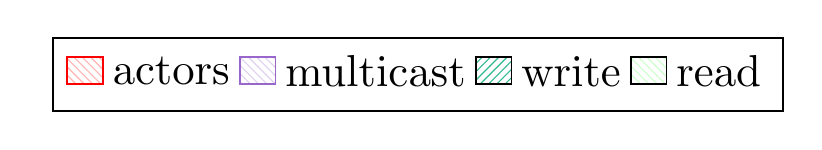
\begin{tikzpicture}
		\legendGantts
	\end{tikzpicture}
  };
}

\newcommand{\KernelScheduledMRB}{
  \node at (14,-3){
	\begin{tikzpicture}
  	   \gantChartUtilizationMRB
	\end{tikzpicture}
  };

  \node at (26,-3){
	\begin{tikzpicture}
  	   \gantChartUtilizationMRBNoReads
	\end{tikzpicture}
  };

  \node at (20,-7){
	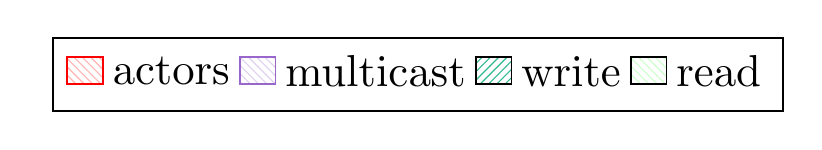
\begin{tikzpicture}
		\legendGantts
	\end{tikzpicture}
  };

}


\newcommand{\HypervolumeResults}{
\pgfplotsset{every tick label/.append style={font=\Large}}
\pgfplotsset{samples=200}
\begin{groupplot}[  
                    group style={
                    group name                 = MemoryFooprintDominance,
%                    group size                 = 2 by 2,
                    group size                 = 3 by 1,
                    xlabels at                 = edge bottom,
                    ylabels at                 = edge left,
%		    vertical sep=1.7cm,
%                   vertical sep=2cm,
%                   horizontal sep=3cm,
                    },
                    height                     = 7cm,
                    xlabel                     = {\Large Generation},
                    ylabel                     = {\Large hypervolume},
                    legend style               = {at={(0.875,-0.25)}, minimum height=0.85cm},
%                    legend style               = {at={(1.35,-0.25)}, minimum height=0.85cm},
                    legend columns             = 6,
%                   legend columns             = 3,
                    ymajorgrids                = true,
                    xmajorgrids                = true,
                    grid style                 = dashed,
		    xtick={0,500,1500,2500},
		    ymin=0,
                  ]

  \nextgroupplot[title=\Large Sobel,xmax=3000]
%     \addplot[ILPDRAMSP,each nth point={25}] table[x index=0,y expr={{1-\thisrowno{6}}} , col sep =tab]{hypervolume/sobel-sequential/results/ILP-sobel-sequential.stats};
%     \addplot[ILPDRAMSPMergingAlways,each nth point={25}] table[x index=0, y expr={{1-\thisrowno{6}}} , col sep =tab] {hypervolume/sobel-sequential/results/ILP-sobel-sequential-always-MRB.stats};
%     \addplot[ILPDRAMSPMergingExplore,each nth point={25}] table[x index=0, y expr={{1-\thisrowno{6}}} , col sep =tab]{hypervolume/sobel-sequential/results/ILP-sobel-sequential-explore-MRB.stats};
%

     \addplot[name path=SSHReference,ILPDRAMSP,each nth point={25}] table[x index=0,y expr={{1-\thisrowno{6}}} , col sep =tab]               {hypervolume/sobel-sequential-transformer/results/ILP-Transformer-sobel-sequential.stats};
     \addplot[ILPDRAMSPMergingAlways,each nth point={25}] table[x index=0, y expr={{1-\thisrowno{6}}} , col sep =tab] {hypervolume/sobel-sequential-transformer/results/ILP-Transformer-sobel-sequential-always-MRB.stats};
     \addplot[name path=SSHExplore,ILPDRAMSPMergingExplore,each nth point={25}] table[x index=0, y expr={{1-\thisrowno{6}}} , col sep =tab]{hypervolume/sobel-sequential-transformer/results/ILP-Transformer-sobel-sequential-explore-MRB.stats};

% Heuristic Initial Token Random Priority
%     \addplot[DRAMSP,each nth point={25}] table[x index=0,y expr={{1-\thisrowno{6}}}, col sep =tab]               {hypervolume/sobel-sequential-transformer/results/Heuristic-Transformer-sobel-sequential.stats};
%     \addplot[DRAMSPMergingAlways,each nth point={25}] table[x index=0, y expr={{1-\thisrowno{6}}}, col sep =tab] {hypervolume/sobel-sequential-transformer/results/Heuristic-Transformer-sobel-sequential-always-MRB.stats};
%     \addplot[DRAMSPMergingExplore,each nth point={25}] table[x index=0, y expr={{1-\thisrowno{6}}}, col sep =tab]{hypervolume/sobel-sequential-transformer/results/Heuristic-Transformer-sobel-sequential-explore-MRB.stats};

% Heuristic no-initial Tokens
%     \addplot[DRAMSP,each nth point={25}] table[x index=0,y expr={{1-\thisrowno{6}}}, col sep =tab]{hypervolume/sobel-sequential-transformer/results/BindingsDSE-sobel-sequential.stats};
%     \addplot[DRAMSPMergingAlways,each nth point={25}] table[x index=0, y expr={{1-\thisrowno{6}}}, col sep =tab]{hypervolume/sobel-sequential-transformer/results/BindingsDSE-sobel-sequential-always-MRB.stats};
%     \addplot[DRAMSPMergingExplore,each nth point={25}] table[x index=0, y expr={{1-\thisrowno{6}}}, col sep =tab]{hypervolume/sobel-sequential-transformer/results/BindingsDSE-sobel-sequential-explore-MRB.stats};
%


% Heuristic Initial Token Topological Priority
%     \addplot[HeuristicTopologicalInit,each nth point={25}] table[x index=0,y expr={{1-\thisrowno{6}}}, col sep =tab]        {hypervolume/sobel-sequential-transformer/results/Sorting-Topological-sobel-sequential.stats};
%     \addplot[HeuristicTopologicalInitAlways,each nth point={25}] table[x index=0, y expr={{1-\thisrowno{6}}}, col sep =tab] {hypervolume/sobel-sequential-transformer/results/Sorting-Topological-sobel-sequential-always-MRB.stats};
%     \addplot[HeuristicTopologicalInitExplore,each nth point={25}] table[x index=0, y expr={{1-\thisrowno{6}}}, col sep =tab]{hypervolume/sobel-sequential-transformer/results/Sorting-Topological-sobel-sequential-explore-MRB.stats};

    \addplot[opacity=0.5,green!50] fill between[of=SSHReference and SSHExplore, soft clip={domain=2300:2500}];

% Heuristic Initial Token Inverse Topological Priority
     \addplot[DRAMSP,each nth point={25}] table[x index=0,y expr={{1-\thisrowno{6}}}, col sep =tab]        {hypervolume/sobel-sequential-transformer/results/Sorting-Inverse-sobel-sequential.stats};
     \addplot[DRAMSPMergingAlways,each nth point={25}] table[x index=0, y expr={{1-\thisrowno{6}}}, col sep =tab] {hypervolume/sobel-sequential-transformer/results/Sorting-Inverse-sobel-sequential-always-MRB.stats};
     \addplot[DRAMSPMergingExplore,each nth point={25}] table[x index=0, y expr={{1-\thisrowno{6}}}, col sep =tab]{hypervolume/sobel-sequential-transformer/results/Sorting-Inverse-sobel-sequential-explore-MRB.stats};

  \nextgroupplot[title=\Large Sobel$_4$,xmax=3000]
%     \addplot[name path=SPHReference,ILPDRAMSP,each nth point={25}] table[x index=0, y expr={{1-\thisrowno{6}}}, col sep =tab]              {hypervolume/sobel-parallel/results/ILP-sobel-parallel4.stats};
%     \addplot[ILPDRAMSPMergingAlways,each nth point={25}] table[x index=0,y expr={{1-\thisrowno{6}}} , col sep =tab] {hypervolume/sobel-parallel/results/ILP-sobel-parallel4-always-MRB.stats};
%     \addplot[name path=SPHExplore,ILPDRAMSPMergingExplore,each nth point={25}] table[x index=0, y expr={{1-\thisrowno{6}}}, col sep =tab]{hypervolume/sobel-parallel/results/ILP-sobel-parallel4-explore-MRB.stats};
%
%     \addplot[DRAMSP,each nth point={25}] table[x index=0, y expr={{1-\thisrowno{6}}} , col sep =tab]              {hypervolume/sobel-parallel/results/BindingsDSE-sobel-parallel4.stats};
%     \addplot[DRAMSPMergingAlways,each nth point={25}] table[x index=0, y expr={{1-\thisrowno{6}}}, col sep =tab] {hypervolume/sobel-parallel/results/BindingsDSE-sobel-parallel4-always-MRB.stats};
%     \addplot[DRAMSPMergingExplore,each nth point={25}] table[x index=0, y expr={{1-\thisrowno{6}}}, col sep =tab]{hypervolume/sobel-parallel/results/BindingsDSE-sobel-parallel4-explore-MRB.stats};

     \addplot[name path=SPHReference,ILPDRAMSP,each nth point={25}] table[x index=0, y expr={{1-\thisrowno{6}}}, col sep =tab]            {hypervolume/sobel-parallel-transformer/results/ILP-Transformer-sobel-parallel4.stats};
     \addplot[ILPDRAMSPMergingAlways,each nth point={25}] table[x index=0,y expr={{1-\thisrowno{6}}} , col sep =tab]                      {hypervolume/sobel-parallel-transformer/results/ILP-Transformer-sobel-parallel4-always-MRB.stats};
     \addplot[name path=SPHExplore,ILPDRAMSPMergingExplore,each nth point={25}] table[x index=0, y expr={{1-\thisrowno{6}}}, col sep =tab]{hypervolume/sobel-parallel-transformer/results/ILP-Transformer-sobel-parallel4-explore-MRB.stats};

% Heuristic Initial Token Random Priority
%     \addplot[DRAMSP,each nth point={25}] table[x index=0, y expr={{1-\thisrowno{6}}} , col sep =tab]             {hypervolume/sobel-parallel-transformer/results/Heuristic-Transformer-sobel-parallel4.stats};
%     \addplot[DRAMSPMergingAlways,each nth point={25}] table[x index=0, y expr={{1-\thisrowno{6}}}, col sep =tab] {hypervolume/sobel-parallel-transformer/results/Heuristic-Transformer-sobel-parallel4-always-MRB.stats};
%     \addplot[DRAMSPMergingExplore,each nth point={25}] table[x index=0, y expr={{1-\thisrowno{6}}}, col sep =tab]{hypervolume/sobel-parallel-transformer/results/Heuristic-Transformer-sobel-parallel4-explore-MRB.stats};

% Heuristic no-initial Tokens
%     \addplot[DRAMSP,each nth point={25}] table[x index=0, y expr={{1-\thisrowno{6}}} , col sep =tab]             {hypervolume/sobel-parallel-transformer/results/BindingsDSE-sobel-parallel4.stats};
%     \addplot[DRAMSPMergingAlways,each nth point={25}] table[x index=0, y expr={{1-\thisrowno{6}}}, col sep =tab] {hypervolume/sobel-parallel-transformer/results/BindingsDSE-sobel-parallel4-always-MRB.stats};
%     \addplot[DRAMSPMergingExplore,each nth point={25}] table[x index=0, y expr={{1-\thisrowno{6}}}, col sep =tab]{hypervolume/sobel-parallel-transformer/results/BindingsDSE-sobel-parallel4-explore-MRB.stats};

% Heuristic Initial Token Topological Priority
%     \addplot[HeuristicTopologicalInit,each nth point={25}] table[x index=0, y expr={{1-\thisrowno{6}}} , col sep =tab]      {hypervolume/sobel-parallel-transformer/results/Sorting-Topological-sobel-parallel4.stats};
%     \addplot[HeuristicTopologicalInitAlways,each nth point={25}] table[x index=0, y expr={{1-\thisrowno{6}}}, col sep =tab] {hypervolume/sobel-parallel-transformer/results/Sorting-Topological-sobel-parallel4-always-MRB.stats};
%     \addplot[HeuristicTopologicalInitExplore,each nth point={25}] table[x index=0, y expr={{1-\thisrowno{6}}}, col sep =tab]{hypervolume/sobel-parallel-transformer/results/Sorting-Topological-sobel-parallel4-explore-MRB.stats};
%
% Heuristic Initial Token Inverse Topological Priority
     \addplot[DRAMSP,each nth point={25}] table[x index=0, y expr={{1-\thisrowno{6}}} , col sep =tab]      {hypervolume/sobel-parallel-transformer/results/Sorting-Inverse-sobel-parallel4.stats};
     \addplot[DRAMSPMergingAlways,each nth point={25}] table[x index=0, y expr={{1-\thisrowno{6}}}, col sep =tab] {hypervolume/sobel-parallel-transformer/results/Sorting-Inverse-sobel-parallel4-always-MRB.stats};
     \addplot[DRAMSPMergingExplore,each nth point={25}] table[x index=0, y expr={{1-\thisrowno{6}}}, col sep =tab]{hypervolume/sobel-parallel-transformer/results/Sorting-Inverse-sobel-parallel4-explore-MRB.stats};

    \addplot[opacity=0.5,green!50] fill between[of=SPHReference and SPHExplore, soft clip={domain=2300:2500}];


  \nextgroupplot[title=\Large Multicamera,xmax=3000 ]
%  \nextgroupplot[title=\Large Multicamera,xmax=3000,xshift=5cm ]
    \addlegendimage{ILPDRAMSP}
    \addlegendentry{\Large $\Reference^{ILP}$}
    \addlegendimage{ILPDRAMSPMergingAlways}
    \addlegendentry{\Large $\MergingAlways^{ILP}$}
    \addlegendimage{ILPDRAMSPMergingExplore }
    \addlegendentry{\Large $\MergingExplore^{ILP}$}
    \addlegendimage{DRAMSP}
    \addlegendentry{\Large $\Reference^{\fHeuristic}$}
    \addlegendimage{DRAMSPMergingAlways}
    \addlegendentry{\Large $\MergingAlways^{\fHeuristic}$}
    \addlegendimage{DRAMSPMergingExplore }
    \addlegendentry{\Large $\MergingExplore^{\fHeuristic}$}

    \addplot[name path=PRILP,ILPDRAMSP,each nth point={25}] table[x index=0, y expr={{1-\thisrowno{6}}} , col sep =tab]          {hypervolume/multicamera-1instance-transformer/results/ILP-Transformer-multicamera.stats};
    \addplot[ILPDRAMSPMergingAlways,each nth point={25}] table[x index=0, y expr={{1-\thisrowno{6}}} , col sep =tab]               {hypervolume/multicamera-1instance-transformer/results/ILP-Transformer-multicamera-always-MRB.stats};
    \addplot[name path=PEIP,ILPDRAMSPMergingExplore,each nth point={25}] table[x index=0, y expr={{1-\thisrowno{6}}}, col sep =tab]{hypervolume/multicamera-1instance-transformer/results/ILP-Transformer-multicamera-explore-MRB.stats};

% Heuristic Initial Token Random Priority
%    \addplot[name path=MHReference,DRAMSP,each nth point={25}] table[x index=0, y expr={{1-\thisrowno{6}}}, col sep =tab]            {hypervolume/multicamera-1instance-transformer/results/Heuristic-Transformer-multicamera-1instance.stats};
%    \addplot[DRAMSPMergingAlways,each nth point={25}] table[x index=0, y expr={{1-\thisrowno{6}}}, col sep =tab]                     {hypervolume/multicamera-1instance-transformer/results/Heuristic-Transformer-multicamera-1instance-always-MRB.stats};
%    \addplot[name path=MHExplore,DRAMSPMergingExplore,each nth point={25}] table[x index=0, y expr={{1-\thisrowno{6}}}, col sep =tab]{hypervolume/multicamera-1instance-transformer/results/Heuristic-Transformer-multicamera-1instance-explore-MRB.stats};

% Heuristic no-Initial Tokens
%    \addplot[name path=MHReference,DRAMSP,each nth point={25}] table[x index=0, y expr={{1-\thisrowno{6}}}, col sep =tab]            {hypervolume/multicamera-1instance-transformer/results/BindingsDSE-multicamera-1instance.stats};
%    \addplot[DRAMSPMergingAlways,each nth point={25}] table[x index=0, y expr={{1-\thisrowno{6}}}, col sep =tab]                     {hypervolume/multicamera-1instance-transformer/results/BindingsDSE-multicamera-1instance-always-MRB.stats};
%    \addplot[name path=MHExplore,DRAMSPMergingExplore,each nth point={25}] table[x index=0, y expr={{1-\thisrowno{6}}}, col sep =tab]{hypervolume/multicamera-1instance-transformer/results/BindingsDSE-multicamera-1instance-explore-MRB.stats};

% Heuristic Initial Token Random Priority
%    \addplot[HeuristicTopologicalInit,each nth point={25}] table[x index=0, y expr={{1-\thisrowno{6}}}, col sep =tab]       {hypervolume/multicamera-1instance-transformer/results/Sorting-Topological-multicamera-1instance.stats};
%    \addplot[HeuristicTopologicalInitAlways,each nth point={25}] table[x index=0, y expr={{1-\thisrowno{6}}}, col sep =tab] {hypervolume/multicamera-1instance-transformer/results/Sorting-Topological-multicamera-1instance-always-MRB.stats};
%    \addplot[HeuristicTopologicalInitExplore,each nth point={25}] table[x index=0, y expr={{1-\thisrowno{6}}}, col sep =tab]{hypervolume/multicamera-1instance-transformer/results/Sorting-Topological-multicamera-1instance-explore-MRB.stats};

% Heuristic Initial Token Inverse Topological Priority
    \addplot[DRAMSP, name path=MHReference,  each nth point={25}] table[x index=0, y expr={{1-\thisrowno{6}}}, col sep =tab]       {hypervolume/multicamera-1instance-transformer/results/Sorting-Inverse-multicamera-1instance.stats};
    \addplot[DRAMSPMergingAlways,each nth point={25}] table[x index=0, y expr={{1-\thisrowno{6}}}, col sep =tab] {hypervolume/multicamera-1instance-transformer/results/Sorting-Inverse-multicamera-1instance-always-MRB.stats};
    \addplot[DRAMSPMergingExplore,name path=MHExplore, each nth point={25}] table[x index=0, y expr={{1-\thisrowno{6}}}, col sep =tab]{hypervolume/multicamera-1instance-transformer/results/Sorting-Inverse-multicamera-1instance-explore-MRB.stats};

    \addplot[opacity=0.5,green!50] fill between[of=MHExplore and MHReference, soft clip={domain=2300:2500}];

\end{groupplot}

\draw [line width=0.25mm,color=black,decorate,decoration={brace,amplitude=5pt,raise=4pt,mirror},yshift=0pt] (5.3,3.75) -- (5.3,5) node [black,midway,xshift=0.8cm,yshift=0cm] { \large $28\,\%$ };

\draw [line width=0.25mm,color=black,decorate,decoration={brace,amplitude=5pt,raise=4pt,mirror},yshift=0pt] (12.9,2.75) -- (12.9,5) node [black,midway,xshift=0.8cm,yshift=0cm] { \large $66\,\%$ };
\draw [line width=0.25mm,color=black,decorate,decoration={brace,amplitude=5pt,raise=4pt,mirror},yshift=0pt] (20.4,2.5) -- (20.4,5) node [black,midway,xshift=0.8cm,yshift=0cm] { \large $90\,\%$ };

%\draw [line width=0.25mm,color=black,decorate,decoration={brace,amplitude=5pt,raise=4pt,mirror},yshift=0pt] (14.9,2.75) -- (14.9,5) node [black,midway,xshift=0.8cm,yshift=0cm] { \large $33\,\%$ };
%\draw [line width=0.25mm,color=black,decorate,decoration={brace,amplitude=5pt,raise=4pt,mirror},yshift=0pt] (10.4,-5) -- (10.4,-2.5) node [black,midway,xshift=0.8cm,yshift=0cm] { \large $45\,\%$ };

}

\newcommand{\HypervolumeOtherApps}{
\pgfplotsset{every tick label/.append style={font=\Large}}
\pgfplotsset{samples=200}
\begin{groupplot}[  
                    group style={
                    group name                 = MemoryFooprintDominance,
                    group size                 = 4 by 2,
                    xlabels at                 = edge bottom,
                    ylabels at                 = edge left,
		    vertical sep=1.7cm,
                    },
                    height                     = 7cm,
                    %width                      = 6.5cm,
                    xlabel                     = {\Large Generation},
                    ylabel                     = {\Large hypervolume},
                    legend style               = {at={(0.0,-0.25)}, minimum height=0.85cm},
                    legend columns             = 6,
                    ymajorgrids                = true,
                    xmajorgrids                = true,
                    grid style                 = dashed,
		    xtick={0,500,1500,2500},
		    ymin=0,
                  ]

  \nextgroupplot[title=\Large Foreground]
     \addplot[ILPDRAMSP,each nth point={25}] table[x index=0,y expr={{1-\thisrowno{6}}} , col sep =tab]               {hypervolume/foreground-1instance/results/ILP-foreground-1instance.stats};
     \addplot[ILPDRAMSPMergingAlways,each nth point={25}] table[x index=0, y expr={{1-\thisrowno{6}}} , col sep =tab] {hypervolume/foreground-1instance/results/ILP-foreground-1instance-always-MRB.stats};
     \addplot[ILPDRAMSPMergingExplore,each nth point={25}] table[x index=0, y expr={{1-\thisrowno{6}}} , col sep =tab]{hypervolume/foreground-1instance/results/ILP-foreground-1instance-explore-MRB.stats};

     \addplot[DRAMSP,each nth point={25}] table[x index=0,y expr={{1-\thisrowno{6}}}, col sep =tab]               {hypervolume/foreground-1instance/results/BindingsDSE-foreground-1instance.stats};
     \addplot[DRAMSPMergingAlways,each nth point={25}] table[x index=0, y expr={{1-\thisrowno{6}}}, col sep =tab] {hypervolume/foreground-1instance/results/BindingsDSE-foreground-1instance-always-MRB.stats};
     \addplot[DRAMSPMergingExplore,each nth point={25}] table[x index=0, y expr={{1-\thisrowno{6}}}, col sep =tab]{hypervolume/foreground-1instance/results/BindingsDSE-foreground-1instance-explore-MRB.stats};

  \nextgroupplot[title=\Large 4-Foreground]
     \addplot[ILPDRAMSP,each nth point={25}] table[x index=0, y expr={{1-\thisrowno{6}}}, col sep =tab]              {hypervolume/foreground-4instances/results/ILP-foreground-4instances.stats};
     \addplot[ILPDRAMSPMergingAlways,each nth point={25}] table[x index=0,y expr={{1-\thisrowno{6}}} , col sep =tab] {hypervolume/foreground-4instances/results/ILP-foreground-4instances-always-MRB.stats};
     \addplot[ILPDRAMSPMergingExplore,each nth point={25}] table[x index=0, y expr={{1-\thisrowno{6}}}, col sep =tab]{hypervolume/foreground-4instances/results/ILP-foreground-4instances-explore-MRB.stats};

     \addplot[DRAMSP,each nth point={25}] table[x index=0, y expr={{1-\thisrowno{6}}} , col sep =tab]             {hypervolume/foreground-4instances/results/BindingsDSE-foreground-4instances.stats};
     \addplot[DRAMSPMergingAlways,each nth point={25}] table[x index=0, y expr={{1-\thisrowno{6}}}, col sep =tab] {hypervolume/foreground-4instances/results/BindingsDSE-foreground-4instances-always-MRB.stats};
     \addplot[DRAMSPMergingExplore,each nth point={25}] table[x index=0, y expr={{1-\thisrowno{6}}}, col sep =tab]{hypervolume/foreground-4instances/results/BindingsDSE-foreground-4instances-explore-MRB.stats};

%  \nextgroupplot[title=\Large 2-Foreground]
%     \addplot[ILPDRAMSP,each nth point={25}] table[x index=0, y expr={{1-\thisrowno{6}}}, col sep =tab]              {hypervolume/foreground-2instances/results/ILP-foreground-2instances.stats};
%     \addplot[ILPDRAMSPMergingAlways,each nth point={25}] table[x index=0,y expr={{1-\thisrowno{6}}} , col sep =tab] {hypervolume/foreground-2instances/results/ILP-foreground-2instances-always-MRB.stats};
%     \addplot[ILPDRAMSPMergingExplore,each nth point={25}] table[x index=0, y expr={{1-\thisrowno{6}}}, col sep =tab]{hypervolume/foreground-2instances/results/ILP-foreground-2instances-explore-MRB.stats};
%
%     \addplot[DRAMSP,each nth point={25}] table[x index=0, y expr={{1-\thisrowno{6}}} , col sep =tab]             {hypervolume/foreground-2instances/results/BindingsDSE-foreground-2instances.stats};
%     \addplot[DRAMSPMergingAlways,each nth point={25}] table[x index=0, y expr={{1-\thisrowno{6}}}, col sep =tab] {hypervolume/foreground-2instances/results/BindingsDSE-foreground-2instances-always-MRB.stats};
%     \addplot[DRAMSPMergingExplore,each nth point={25}] table[x index=0, y expr={{1-\thisrowno{6}}}, col sep =tab]{hypervolume/foreground-2instances/results/BindingsDSE-foreground-2instances-explore-MRB.stats};


  \nextgroupplot[title=\Large Optical flow]
     \addplot[ILPDRAMSP,each nth point={25}] table[x index=0, y expr={{1-\thisrowno{6}}}, col sep =tab]              {hypervolume/optical-flow-1instance/results/ILP-optical-flow-1instance.stats};
     \addplot[ILPDRAMSPMergingAlways,each nth point={25}] table[x index=0,y expr={{1-\thisrowno{6}}} , col sep =tab] {hypervolume/optical-flow-1instance/results/ILP-optical-flow-1instance-always-MRB.stats};
     \addplot[ILPDRAMSPMergingExplore,each nth point={25}] table[x index=0, y expr={{1-\thisrowno{6}}}, col sep =tab]{hypervolume/optical-flow-1instance/results/ILP-optical-flow-1instance-explore-MRB.stats};

     \addplot[DRAMSP,each nth point={25}] table[x index=0, y expr={{1-\thisrowno{6}}} , col sep =tab]             {hypervolume/optical-flow-1instance/results/BindingsDSE-optical-flow-1instance.stats};
     \addplot[DRAMSPMergingAlways,each nth point={25}] table[x index=0, y expr={{1-\thisrowno{6}}}, col sep =tab] {hypervolume/optical-flow-1instance/results/BindingsDSE-optical-flow-1instance-always-MRB.stats};
     \addplot[DRAMSPMergingExplore,each nth point={25}] table[x index=0, y expr={{1-\thisrowno{6}}}, col sep =tab]{hypervolume/optical-flow-1instance/results/BindingsDSE-optical-flow-1instance-explore-MRB.stats};

  \nextgroupplot[title=\Large 2-Optical flow]
     \addplot[ILPDRAMSP,each nth point={25}] table[x index=0, y expr={{1-\thisrowno{6}}}, col sep =tab]              {hypervolume/optical-flow-2instances/results/ILP-optical-flow-2instances.stats};
     \addplot[ILPDRAMSPMergingAlways,each nth point={25}] table[x index=0,y expr={{1-\thisrowno{6}}} , col sep =tab] {hypervolume/optical-flow-2instances/results/ILP-optical-flow-2instances-always-MRB.stats};
     \addplot[ILPDRAMSPMergingExplore,each nth point={25}] table[x index=0, y expr={{1-\thisrowno{6}}}, col sep =tab]{hypervolume/optical-flow-2instances/results/ILP-optical-flow-2instances-explore-MRB.stats};

     \addplot[DRAMSP,each nth point={25}] table[x index=0, y expr={{1-\thisrowno{6}}} , col sep =tab]             {hypervolume/optical-flow-2instances/results/BindingsDSE-optical-flow-2instances.stats};
     \addplot[DRAMSPMergingAlways,each nth point={25}] table[x index=0, y expr={{1-\thisrowno{6}}}, col sep =tab] {hypervolume/optical-flow-2instances/results/BindingsDSE-optical-flow-2instances-always-MRB.stats};
     \addplot[DRAMSPMergingExplore,each nth point={25}] table[x index=0, y expr={{1-\thisrowno{6}}}, col sep =tab]{hypervolume/optical-flow-2instances/results/BindingsDSE-optical-flow-2instances-explore-MRB.stats};

  \nextgroupplot[title=\Large 3-Optical flow]
     \addplot[ILPDRAMSP,each nth point={25}] table[x index=0, y expr={{1-\thisrowno{6}}}, col sep =tab]              {hypervolume/optical-flow-3instances/results/ILP-optical-flow-3instances.stats};
     \addplot[ILPDRAMSPMergingAlways,each nth point={25}] table[x index=0,y expr={{1-\thisrowno{6}}} , col sep =tab] {hypervolume/optical-flow-3instances/results/ILP-optical-flow-3instances-always-MRB.stats};
     \addplot[ILPDRAMSPMergingExplore,each nth point={25}] table[x index=0, y expr={{1-\thisrowno{6}}}, col sep =tab]{hypervolume/optical-flow-3instances/results/ILP-optical-flow-3instances-explore-MRB.stats};

     \addplot[DRAMSP,each nth point={25}] table[x index=0, y expr={{1-\thisrowno{6}}} , col sep =tab]             {hypervolume/optical-flow-3instances/results/BindingsDSE-optical-flow-3instances.stats};
     \addplot[DRAMSPMergingAlways,each nth point={25}] table[x index=0, y expr={{1-\thisrowno{6}}}, col sep =tab] {hypervolume/optical-flow-3instances/results/BindingsDSE-optical-flow-3instances-always-MRB.stats};
     \addplot[DRAMSPMergingExplore,each nth point={25}] table[x index=0, y expr={{1-\thisrowno{6}}}, col sep =tab]{hypervolume/optical-flow-3instances/results/BindingsDSE-optical-flow-3instances-explore-MRB.stats};

  \nextgroupplot[title=\Large Video]
     \addplot[ILPDRAMSP,each nth point={25}] table[x index=0, y expr={{1-\thisrowno{6}}}, col sep =tab]              {hypervolume/video-1instance/results/ILP-video-object-counting-1instance.stats};
     \addplot[ILPDRAMSPMergingAlways,each nth point={25}] table[x index=0,y expr={{1-\thisrowno{6}}} , col sep =tab] {hypervolume/video-1instance/results/ILP-video-object-counting-1instance-always-MRB.stats};
     \addplot[ILPDRAMSPMergingExplore,each nth point={25}] table[x index=0, y expr={{1-\thisrowno{6}}}, col sep =tab]{hypervolume/video-1instance/results/ILP-video-object-counting-1instance-explore-MRB.stats};

     \addplot[DRAMSP,each nth point={25}] table[x index=0, y expr={{1-\thisrowno{6}}} , col sep =tab]             {hypervolume/video-1instance/results/BindingsDSE-video-object-counting-1instance.stats};
     \addplot[DRAMSPMergingAlways,each nth point={25}] table[x index=0, y expr={{1-\thisrowno{6}}}, col sep =tab] {hypervolume/video-1instance/results/BindingsDSE-video-object-counting-1instance-always-MRB.stats};
     \addplot[DRAMSPMergingExplore,each nth point={25}] table[x index=0, y expr={{1-\thisrowno{6}}}, col sep =tab]{hypervolume/video-1instance/results/BindingsDSE-video-object-counting-1instance-explore-MRB.stats};

  \nextgroupplot[title=\Large 2-Video]
     \addplot[ILPDRAMSP,each nth point={25}] table[x index=0, y expr={{1-\thisrowno{6}}}, col sep =tab]              {hypervolume/video-2instances-transformer/results/ILP-Transformer-video-object-counting-2instances.stats};
     \addplot[ILPDRAMSPMergingAlways,each nth point={25}] table[x index=0,y expr={{1-\thisrowno{6}}} , col sep =tab] {hypervolume/video-2instances-transformer/results/ILP-Transformer-video-object-counting-2instances-always-MRB.stats};
     \addplot[ILPDRAMSPMergingExplore,each nth point={25}] table[x index=0, y expr={{1-\thisrowno{6}}}, col sep =tab]{hypervolume/video-2instances-transformer/results/ILP-Transformer-video-object-counting-2instances-explore-MRB.stats};

     \addplot[DRAMSP,each nth point={25}] table[x index=0, y expr={{1-\thisrowno{6}}} , col sep =tab]             {hypervolume/video-2instances-transformer/results/Heuristic-Transformer-video-object-counting-2instances.stats};
     \addplot[DRAMSPMergingAlways,each nth point={25}] table[x index=0, y expr={{1-\thisrowno{6}}}, col sep =tab] {hypervolume/video-2instances-transformer/results/Heuristic-Transformer-video-object-counting-2instances-always-MRB.stats};
     \addplot[DRAMSPMergingExplore,each nth point={25}] table[x index=0, y expr={{1-\thisrowno{6}}}, col sep =tab]{hypervolume/video-2instances-transformer/results/Heuristic-Transformer-video-object-counting-2instances-explore-MRB.stats};

  \nextgroupplot[title=\Large 3-Video]
    \addlegendimage{ILPDRAMSP}
    \addlegendentry{\Large $\Reference^{ILP}$}
    \addlegendimage{ILPDRAMSPMergingAlways}
    \addlegendentry{\Large $\MergingAlways^{ILP}$}
    \addlegendimage{ILPDRAMSPMergingExplore }
    \addlegendentry{\Large $\MergingExplore^{ILP}$}
    \addlegendimage{DRAMSP}
    \addlegendentry{\Large $\Reference^{\fHeuristic}$}
    \addlegendimage{DRAMSPMergingAlways}
    \addlegendentry{\Large $\MergingAlways^{\fHeuristic}$}
    \addlegendimage{DRAMSPMergingExplore }
    \addlegendentry{\Large $\MergingExplore^{\fHeuristic}$}
     \addplot[ILPDRAMSP,each nth point={25}] table[x index=0, y expr={{1-\thisrowno{6}}}, col sep =tab]              {hypervolume/video-3instances/results/ILP-video-object-counting-3instances.stats};
     \addplot[ILPDRAMSPMergingAlways,each nth point={25}] table[x index=0,y expr={{1-\thisrowno{6}}} , col sep =tab] {hypervolume/video-3instances/results/ILP-video-object-counting-3instances-always-MRB.stats};
     \addplot[ILPDRAMSPMergingExplore,each nth point={25}] table[x index=0, y expr={{1-\thisrowno{6}}}, col sep =tab]{hypervolume/video-3instances/results/ILP-video-object-counting-3instances-explore-MRB.stats};

     \addplot[DRAMSP,each nth point={25}] table[x index=0, y expr={{1-\thisrowno{6}}} , col sep =tab]             {hypervolume/video-3instances/results/BindingsDSE-video-object-counting-3instances.stats};
     \addplot[DRAMSPMergingAlways,each nth point={25}] table[x index=0, y expr={{1-\thisrowno{6}}}, col sep =tab] {hypervolume/video-3instances/results/BindingsDSE-video-object-counting-3instances-always-MRB.stats};
     \addplot[DRAMSPMergingExplore,each nth point={25}] table[x index=0, y expr={{1-\thisrowno{6}}}, col sep =tab]{hypervolume/video-3instances/results/BindingsDSE-video-object-counting-3instances-explore-MRB.stats};

\end{groupplot}

}


%\newcommand{\HypervolumeResultsB}{
%\pgfplotsset{every tick label/.append style={font=\Large}}
%\pgfplotsset{samples=200}
%\begin{groupplot}[  
%                    group style={
%                    group name                 = MemoryFooprintDominance,
%                    group size                 = 4 by 2,
%                    xlabels at                 = edge bottom,
%                    ylabels at                 = edge left,
%		    vertical sep=1.7cm,
%                    },
%                    %height                     = 5cm,
%                    %width                      = 6.5cm,
%                    xlabel                     = {\Large Generation $i$},
%                    ylabel                     = {\Large hypervolume},
%                    legend style               = {at={(-0.6,-0.25)}},
%                    legend columns             = 3,
%                    ymajorgrids                = true,
%                    xmajorgrids                = true,
%                    grid style                 = dashed,
%		    xtick={0,1000,2000,3000},
%                  ]
%
%    \nextgroupplot[title=\Large Optical Flow 3]
%       \addplot[DRAMSP] table[x index=0, y expr = 1-\thisrowno{6}  , col sep =tab]             {edominance/architecture-4tiles/optical-flow/results/optical-flow.stats};
%       \addplot[DRAMSPMergingAlways] table[x index=0, y expr = 1-\thisrowno{6} , col sep =tab] {edominance/architecture-4tiles/optical-flow/results/optical-flow-always-MRB.stats};
%       \addplot[DRAMSPMergingExplore] table[x index=0, y expr = 1-\thisrowno{6} , col sep =tab]{edominance/architecture-4tiles/optical-flow/results/optical-flow-explore-MRB.stats};
%
%    \nextgroupplot[title=\Large Optical Flow 2]
%       \addplot[DRAMSP] table[x index=0, y expr = 1-\thisrowno{6}  , col sep =tab]             {edominance/architecture-4tiles/optical-flow-2instances/results/optical-flow-2instances.stats};
%       \addplot[DRAMSPMergingAlways] table[x index=0, y expr = 1-\thisrowno{6} , col sep =tab] {edominance/architecture-4tiles/optical-flow-2instances/results/optical-flow-2instances-always-MRB.stats};
%       \addplot[DRAMSPMergingExplore] table[x index=0, y expr = 1-\thisrowno{6} , col sep =tab]{edominance/architecture-4tiles/optical-flow-2instances/results/optical-flow-2instances-explore-MRB.stats};
%
%
%    \nextgroupplot[title=\Large Video Object Counting 5]
%%       \addplot[DRAMSP] table[x index=0, y expr = 1-\thisrowno{6}  , col sep =tab]             {edominance/architecture-4tiles/video/results/video-object-counting.stats};
%%       \addplot[DRAMSPMergingAlways] table[x index=0, y expr = 1-\thisrowno{6} , col sep =tab] {edominance/architecture-4tiles/video/results/video-object-counting-always-MRB.stats};
%%       \addplot[DRAMSPMergingExplore] table[x index=0, y expr = 1-\thisrowno{6} , col sep =tab]{edominance/architecture-4tiles/video/results/video-object-counting-explore-MRB.stats};
%
%
%    \nextgroupplot[title=\Large Sobel Sequential 5]
%       \addplot[DRAMSP] table[x index=0, y expr = 1-\thisrowno{6}  , col sep =tab]              {edominance/architecture-4tiles/sobel-sequential-5instances/results/sobel-sequential-instances5.stats};
%       \addplot[DRAMSPMergingAlways] table[x index=0, y expr = 1-\thisrowno{6}  , col sep =tab] {edominance/architecture-4tiles/sobel-sequential-5instances/results/sobel-sequential-instances5-always-MRB.stats};
%       \addplot[DRAMSPMergingExplore] table[x index=0, y expr = 1-\thisrowno{6}  , col sep =tab]{edominance/architecture-4tiles/sobel-sequential-5instances/results/sobel-sequential-instances5-explore-MRB.stats};
%
%    \nextgroupplot[title=\Large Sobel Sequential 10]
%       \addplot[DRAMSP] table[x index=0, y expr = 1-\thisrowno{6}  , col sep =tab]              {edominance/architecture-4tiles/sobel-sequential-10instances/results/sobel-sequential-instances10.stats};
%       \addplot[DRAMSPMergingAlways] table[x index=0, y expr = 1-\thisrowno{6}  , col sep =tab] {edominance/architecture-4tiles/sobel-sequential-10instances/results/sobel-sequential-instances10-always-MRB.stats};
%       \addplot[DRAMSPMergingExplore] table[x index=0, y expr = 1-\thisrowno{6}  , col sep =tab]{edominance/architecture-4tiles/sobel-sequential-10instances/results/sobel-sequential-instances10-explore-MRB.stats};
%
%   \nextgroupplot[title=\Large Sobel Sequential 20]
%       \addplot[DRAMSP] table[x index=0, y expr = 1-\thisrowno{6}  , col sep =tab]              {edominance/architecture-4tiles/sobel-sequential-20instances/results/sobel-sequential-instances20.stats};
%       \addplot[DRAMSPMergingAlways] table[x index=0, y expr = 1-\thisrowno{6}  , col sep =tab] {edominance/architecture-4tiles/sobel-sequential-20instances/results/sobel-sequential-instances20-always-MRB.stats};
%       \addplot[DRAMSPMergingExplore] table[x index=0, y expr = 1-\thisrowno{6}  , col sep =tab]{edominance/architecture-4tiles/sobel-sequential-20instances/results/sobel-sequential-instances20-explore-MRB.stats};
%
%   \nextgroupplot[title=\Large Sobel Parallel 5]
%       \addplot[DRAMSP] table[x index=0, y expr = 1-\thisrowno{6}  , col sep =tab]              {edominance/architecture-4tiles/sobel-parallel-5instances/results/sobel-parallel4-instances5.stats};
%       \addplot[DRAMSPMergingAlways] table[x index=0, y expr = 1-\thisrowno{6}  , col sep =tab] {edominance/architecture-4tiles/sobel-parallel-5instances/results/sobel-parallel4-instances5-always-MRB.stats};
%       \addplot[DRAMSPMergingExplore] table[x index=0, y expr = 1-\thisrowno{6}  , col sep =tab]{edominance/architecture-4tiles/sobel-parallel-5instances/results/sobel-parallel4-instances5-explore-MRB.stats};
%
%    \nextgroupplot[title=\Large Sobel Parallel 10]
%       \addplot[DRAMSP] table[x index=0, y expr = 1-\thisrowno{6}  , col sep =tab]              {edominance/architecture-4tiles/sobel-parallel-10instances/results/sobel-parallel4-instances10.stats};
%       \addplot[DRAMSPMergingAlways] table[x index=0, y expr = 1-\thisrowno{6}  , col sep =tab] {edominance/architecture-4tiles/sobel-parallel-10instances/results/sobel-parallel4-instances10-always-MRB.stats};
%       \addplot[DRAMSPMergingExplore] table[x index=0, y expr = 1-\thisrowno{6}  , col sep =tab]{edominance/architecture-4tiles/sobel-parallel-10instances/results/sobel-parallel4-instances10-explore-MRB.stats};
%
%\end{groupplot}
%
%}
%
%
%\newcommand{\HypervolumeComparisonResults}{
%\pgfplotsset{every tick label/.append style={font=\Large}}
%\pgfplotsset{samples=200}
%\begin{groupplot}[  
%                    group style={
%                    group name                 = MemoryFooprintDominance,
%                    group size                 = 4 by 2,
%                    xlabels at                 = edge bottom,
%                    ylabels at                 = edge left,
%		    vertical sep=1.7cm,
%                    },
%                    %height                     = 5cm,
%                    %width                      = 6.5cm,
%                    xlabel                     = {\Large Generation $i$},
%                    ylabel                     = {\Large hypervolume},
%                    legend style               = {at={(-0.6,-0.25)}},
%                    legend columns             = 3,
%                    ymajorgrids                = true,
%                    xmajorgrids                = true,
%                    grid style                 = dashed,
%		    xtick={0,1000,2000,3000},
%                  ]
%
%  \nextgroupplot[title=\Large Sobel]
%     \addplot[DRAMSP] table[x index=0, y expr = 1-\thisrowno{6}  , col sep =tab]              {edominance/comparison-approaches/sobel-sequential/results/sobel-sequential.stats};
%     \addplot[DRAMSPMergingAlways] table[x index=0, y expr = 1-\thisrowno{6}  , col sep =tab] {edominance/comparison-approaches/sobel-sequential/results/sobel-sequential-always-MRB.stats};
%     \addplot[DRAMSPMergingExplore] table[x index=0, y expr = 1-\thisrowno{6}  , col sep =tab]{edominance/comparison-approaches/sobel-sequential/results/sobel-sequential-explore-MRB.stats};
%
%     \addplot[DRAMSP,dashed] table[x index=0, y expr = 1-\thisrowno{6}  , col sep =tab]              {edominance/comparison-approaches/sobel-sequential/results/FCFS-sobel-sequential.stats};
%     \addplot[DRAMSPMergingAlways,dashed] table[x index=0, y expr = 1-\thisrowno{6}  , col sep =tab] {edominance/comparison-approaches/sobel-sequential/results/FCFS-sobel-sequential-always-MRB.stats};
%     \addplot[DRAMSPMergingExplore,dashed] table[x index=0, y expr = 1-\thisrowno{6}  , col sep =tab]{edominance/comparison-approaches/sobel-sequential/results/FCFS-sobel-sequential-explore-MRB.stats};
%
%  \nextgroupplot[title=\Large Sobel Parallel]
%%     \addplot[DRAMSP] table[x index=0, y expr = 1-\thisrowno{6}  , col sep =tab]              {edominance/architecture-4tiles/sobel-parallel/results/sobel-parallel4.stats};
%%     \addplot[DRAMSPMergingAlways] table[x index=0, y expr = 1-\thisrowno{6}  , col sep =tab] {edominance/architecture-4tiles/sobel-parallel/results/sobel-parallel4-always-MRB.stats};
%%     \addplot[DRAMSPMergingExplore] table[x index=0, y expr = 1-\thisrowno{6}  , col sep =tab]{edominance/architecture-4tiles/sobel-parallel/results/sobel-parallel4-explore-MRB.stats};
%
%  \nextgroupplot[title=\Large Multicamera ]
%%     \addplot[DRAMSP] table[x index=0, y expr = 1-\thisrowno{6}  , col sep =tab]              {edominance/architecture-4tiles/multicamera-1instance/results/multicamera-1instance.stats};
%%     \addplot[DRAMSPMergingAlways] table[x index=0, y expr = 1-\thisrowno{6} , col sep =tab]  {edominance/architecture-4tiles/multicamera-1instance/results/multicamera-1instance-always-MRB.stats};
%%     \addplot[DRAMSPMergingExplore] table[x index=0, y expr = 1-\thisrowno{6}  , col sep =tab]{edominance/architecture-4tiles/multicamera-1instance/results/multicamera-1instance-explore-MRB.stats};
%
%  \nextgroupplot[title=\Large Multicamera 2]
%%     \addplot[DRAMSP] table[x index=0, y expr = 1-\thisrowno{6} , col sep =tab]               {edominance/architecture-4tiles/multicamera/results/multicamera.stats};
%%     \addplot[DRAMSPMergingAlways] table[x index=0, y expr = 1-\thisrowno{6} , col sep =tab]  {edominance/architecture-4tiles/multicamera/results/multicamera-always-MRB.stats};
%%     \addplot[DRAMSPMergingExplore] table[x index=0, y expr = 1-\thisrowno{6}  , col sep =tab]{edominance/architecture-4tiles/multicamera/results/multicamera-explore-MRB.stats};
%
%
%  \nextgroupplot[title=\Large Multicamera 3]
%%     \addplot[DRAMSP] table[x index=0, y expr = 1-\thisrowno{6}  , col sep =tab]              {edominance/architecture-4tiles/multicamera-3instances/results/multicamera-3instances.stats};
%%     \addplot[DRAMSPMergingAlways] table[x index=0, y expr = 1-\thisrowno{6} , col sep =tab]  {edominance/architecture-4tiles/multicamera-3instances/results/multicamera-3instances-always-MRB.stats};
%%     \addplot[DRAMSPMergingExplore] table[x index=0, y expr = 1-\thisrowno{6}  , col sep =tab]{edominance/architecture-4tiles/multicamera-3instances/results/multicamera-3instances-explore-MRB.stats};
%
%
%
%  \nextgroupplot[title=\Large Foreground 4]
%     \addplot[DRAMSP] table[x index=0, y expr = 1-\thisrowno{6}  , col sep =tab]              {edominance/comparison-approaches/foreground-4instances/results/foreground-4instances.stats};
%     \addplot[DRAMSPMergingAlways] table[x index=0, y expr = 1-\thisrowno{6}  , col sep =tab] {edominance/comparison-approaches/foreground-4instances/results/foreground-4instances-always-MRB.stats};
%     \addplot[DRAMSPMergingExplore] table[x index=0, y expr = 1-\thisrowno{6}  , col sep =tab]{edominance/comparison-approaches/foreground-4instances/results/foreground-4instances-explore-MRB.stats};
%
%     \addplot[DRAMSP,dashed] table[x index=0, y expr = 1-\thisrowno{6}  , col sep =tab]              {edominance/comparison-approaches/foreground-4instances/results/FCFS-foreground-4instances.stats};
%     \addplot[DRAMSPMergingAlways,dashed] table[x index=0, y expr = 1-\thisrowno{6}  , col sep =tab] {edominance/comparison-approaches/foreground-4instances/results/FCFS-foreground-4instances-always-MRB.stats};
%     \addplot[DRAMSPMergingExplore,dashed] table[x index=0, y expr = 1-\thisrowno{6}  , col sep =tab]{edominance/comparison-approaches/foreground-4instances/results/FCFS-foreground-4instances-explore-MRB.stats};
%
%
%  \nextgroupplot[title=\Large Foreground 7]
%%     \addplot[DRAMSP] table[x index=0, y expr = 1-\thisrowno{6}, col sep =tab]                {edominance/architecture-4tiles/foreground/results/foreground.stats};
%%     \addplot[DRAMSPMergingAlways] table[x index=0, y expr = 1-\thisrowno{6}  , col sep =tab] {edominance/architecture-4tiles/foreground/results/foreground-always-MRB.stats};
%%     \addplot[DRAMSPMergingExplore] table[x index=0, y expr = 1-\thisrowno{6}  , col sep =tab]{edominance/architecture-4tiles/foreground/results/foreground-explore-MRB.stats};
%
%
%  \nextgroupplot[title=\Large Video Object Counting 3]
%    \addlegendimage{DRAMSP}
%    \addlegendentry{\Large $\Reference$}
%    \addlegendimage{DRAMSPMergingAlways}
%    \addlegendentry{\Large $\MergingAlways$}
%    \addlegendimage{DRAMSPMergingExplore }
%    \addlegendentry{\Large $\MergingExplore$}
%
%    \addlegendimage{DRAMSP}
%    \addlegendentry{\Large $FCFS$}
%    \addlegendimage{DRAMSPMergingAlways}
%    \addlegendentry{\Large $FCFS_{Always}$}
%    \addlegendimage{DRAMSPMergingExplore }
%    \addlegendentry{\Large $FCFS_{Explore$}}
%
%%     \addplot[DRAMSP] table[x index=0, y expr = 1-\thisrowno{6}  , col sep =tab]             {edominance/architecture-4tiles/video-3instances/results/video-object-counting-3instances.stats};
%%     \addplot[DRAMSPMergingAlways] table[x index=0, y expr = 1-\thisrowno{6} , col sep =tab] {edominance/architecture-4tiles/video-3instances/results/video-object-counting-3instances-always-MRB.stats};
%%     \addplot[DRAMSPMergingExplore] table[x index=0, y expr = 1-\thisrowno{6} , col sep =tab]{edominance/architecture-4tiles/video-3instances/results/video-object-counting-3instances-explore-MRB.stats};
%
%\end{groupplot}
%
%}
%

\newcommand{\ParetoHeuristicBindingsDSE}{
\pgfplotsset{every tick label/.append style={font=\Large}}
\pgfplotsset{samples=200}

\pgfplotsset{
colormap={bluered}{rgb255(0cm)=(0,0,180); rgb255(1cm)=(0,255,255); rgb255(2cm)=(100,255,0);rgb255(3cm)=(255,255,0); rgb255(4cm)=(255,0,0); rgb255(5cm)=(128,0,0)}
%colormap={greenyellow}{rgb255(0cm)=(255,255,0) rgb255(1cm)=(0,128,0) rgb255(2cm)=(0,0,0)},                       
%colormap={discreteMap}{
%rgb255=(255,0,0)       %24
%rgb255=(245,0,112)       %23
%rgb255=(237,0,207)       %22
%rgb255=(233,0,255)       %21
%rgb255=(150,0,255)       %20
%rgb255=(50,0,255)       %19
%rgb255=(0,0,255)       %18
%rgb255=(4,91,249)       %17
%rgb255=(7,164,244)       %16
%rgb255=(0,203,241)       %15
%rgb255=(11,255,238)       %14
%rgb255=(8,255,170)       %13
%rgb255=(4,255,85)       %12
%rgb255=(0,255,0)       %11
%rgb255=(73,255,0)       %10
%rgb255=(255,255,0)       %8
%rgb255=(255,237,0)       %7
%rgb255=(255,192,0)       %6
%rgb255=(255,128,0)       %5
%rgb255=(207,104,0)       %4
%rgb255=(173,87,0)       %3
%%rgb255=(115,58,0)       %2  
%%rgb255=(0,0,0)       %1     
%},                       
}
  \begin{groupplot}[  
                      group style={
                      group name                 = MemoryFooprintDominance,
                      group size                 = 3 by 1,
%                      group size                 = 2 by 2,
                      xlabels at                 = edge bottom,
                      ylabels at                 = edge left,
		      vertical sep=2.5cm,
                      horizontal sep=2.75cm,
%                      vertical sep=3cm,
%                      horizontal sep=4cm,
                      },
                      ylabel                     = {\huge \begin{tabular}{c} $\MemoryFootprint$ [MiB] \end{tabular}},
                      xlabel                     = {\huge \begin{tabular}{c} Period $\Period$ [ms] \end{tabular}},
                      legend style               = {at={(0.25,-0.35)}, minimum height=1.25cm },
%                      legend style               = {at={(1.75,-0.35)}, minimum height=1.25cm },
                      legend columns             = 3,
                      ymajorgrids                = true,
                      xmajorgrids                = true,
                      xmode=log,
                      grid style                 = dashed,
                      colormap name =bluered,
                      colorbar sampled,
                      point meta min=0,
                      point meta max=24,
                    ]

%    \nextgroupplot[title=\huge Sobel Sequential,xmin=0,xmax=75,ymin=50,ymax=150]
    \nextgroupplot[title=\huge Sobel,xmin=0,xmax=80,ymin=40,ymax=170, xtick={0,10,20,40,80}, xticklabels = {10,20,40,80} ]
%	\addplot[ScatterAlways] table[x expr=1000/\thisrowno{0}, y expr=\thisrowno{2}/1024/1024, scatter src=\thisrowno{1}, col sep =tab]{csv/pareto-fronts/ModuloScheduling-BindingsDSE-Sobel-Sequential-Always-Fraction.csv};
%	\addplot[ScatterReference] table[x expr=1000/\thisrowno{0}, y expr=\thisrowno{2}/1024/1024, scatter src=\thisrowno{1}, col sep =tab]{csv/pareto-fronts/ModuloScheduling-BindingsDSE-Sobel-Sequential-Fraction.csv};
%	\addplot[ScatterExplore] table[x expr=1000/\thisrowno{0}, y expr=\thisrowno{2}/1024/1024 , scatter src=\thisrowno{1}, col sep =tab]{csv/pareto-fronts/ModuloScheduling-BindingsDSE-Sobel-Sequential-Explore-Fraction.csv};
%
%	\addplot[NonDominatedAlways] table[x expr=1000/\thisrowno{0}, y expr=\thisrowno{2}/1024/1024, scatter src=\thisrowno{1}, col sep =tab]{csv/pareto-fronts/Global-ModuloScheduling-BindingsDSE-Sobel-Sequential-Distilled-Always.csv};
%	\addplot[NonDominatedReference] table[x expr=1000/\thisrowno{0}, y expr=\thisrowno{2}/1024/1024, scatter src=\thisrowno{1}, col sep =tab]{csv/pareto-fronts/Global-ModuloScheduling-BindingsDSE-Sobel-Sequential-Distilled-Reference.csv};
%	\addplot[NonDominatedExplore] table[x expr=1000/\thisrowno{0}, y expr=\thisrowno{2}/1024/1024 , scatter src=\thisrowno{1}, col sep =tab]{csv/pareto-fronts/Global-ModuloScheduling-BindingsDSE-Sobel-Sequential-Distilled-Explore.csv};

% WITH INITIAL TOKEN
 
	\addplot[ScatterAlways] table[x expr=1000/\thisrowno{0}, y expr=\thisrowno{2}/1024/1024, scatter src=\thisrowno{1}, col sep =tab]{csv/pareto-fronts/TokenModuloScheduling-BindingsDSE-Sobel-Sequential-Always-Fraction.csv};
	\addplot[ScatterReference] table[x expr=1000/\thisrowno{0}, y expr=\thisrowno{2}/1024/1024, scatter src=\thisrowno{1}, col sep =tab]{csv/pareto-fronts/TokenModuloScheduling-BindingsDSE-Sobel-Sequential-Fraction.csv};
	\addplot[ScatterExplore] table[x expr=1000/\thisrowno{0}, y expr=\thisrowno{2}/1024/1024 , scatter src=\thisrowno{1}, col sep =tab]{csv/pareto-fronts/TokenModuloScheduling-BindingsDSE-Sobel-Sequential-Explore-Fraction.csv};

	\addplot[NonDominatedAlways] table[x expr=1000/\thisrowno{0}, y expr=\thisrowno{2}/1024/1024, scatter src=\thisrowno{1}, col sep =tab]{csv/pareto-fronts/Global-TokenModuloScheduling-BindingsDSE-Sobel-Sequential-Distilled-Always.csv};
	\addplot[NonDominatedReference] table[x expr=1000/\thisrowno{0}, y expr=\thisrowno{2}/1024/1024, scatter src=\thisrowno{1}, col sep =tab]{csv/pareto-fronts/Global-TokenModuloScheduling-BindingsDSE-Sobel-Sequential-Distilled-Reference.csv};
	\addplot[NonDominatedExplore] table[x expr=1000/\thisrowno{0}, y expr=\thisrowno{2}/1024/1024 , scatter src=\thisrowno{1}, col sep =tab]{csv/pareto-fronts/Global-TokenModuloScheduling-BindingsDSE-Sobel-Sequential-Distilled-Explore.csv};


    \nextgroupplot[title=\huge Sobel$_4$,xmin=0,xmax=75,ymin=45,ymax=130, xtick = {0,10,20,40,75},xticklabels={10,20,40,75} ,xshift=0.7cm   ]
%      \addplot[ScatterAlways] table[x expr=1000/\thisrowno{0}, y expr=\thisrowno{2}/1024/1024, scatter src=\thisrowno{1}, col sep =tab]{csv/pareto-fronts/ModuloScheduling-BindingsDSE-Sobel-Parallel-Always-Fraction.csv};
%      \addplot[ScatterReference] table[x expr=1000/\thisrowno{0}, y expr=\thisrowno{2}/1024/1024 , scatter src=\thisrowno{1},  col sep =tab]{csv/pareto-fronts/ModuloScheduling-BindingsDSE-Sobel-Parallel-Fraction.csv};
%      \addplot[ScatterExplore] table[x expr=1000/\thisrowno{0}, y expr=\thisrowno{2}/1024/1024,scatter src=\thisrowno{1},  col sep =tab]{csv/pareto-fronts/ModuloScheduling-BindingsDSE-Sobel-Parallel-Explore-Fraction.csv};
%
%      \addplot[NonDominatedAlways] table[x expr=1000/\thisrowno{0}, y expr=\thisrowno{2}/1024/1024, scatter src=\thisrowno{1}, col sep =tab]{csv/pareto-fronts/Global-ModuloScheduling-BindingsDSE-Sobel-Parallel-Distilled-Always.csv};
%      \addplot[NonDominatedReference] table[x expr=1000/\thisrowno{0}, y expr=\thisrowno{2}/1024/1024 , scatter src=\thisrowno{1},  col sep =tab]{csv/pareto-fronts/Global-ModuloScheduling-BindingsDSE-Sobel-Parallel-Distilled-Reference.csv};
%      \addplot[NonDominatedExplore] table[x expr=1000/\thisrowno{0}, y expr=\thisrowno{2}/1024/1024,scatter src=\thisrowno{1},  col sep =tab]{csv/pareto-fronts/Global-ModuloScheduling-BindingsDSE-Sobel-Parallel-Distilled-Explore.csv};

% WITH INITIAL TOKEN

      \addplot[ScatterAlways] table[x expr=1000/\thisrowno{0}, y expr=\thisrowno{2}/1024/1024, scatter src=\thisrowno{1}, col sep =tab]{csv/pareto-fronts/TokenModuloScheduling-BindingsDSE-Sobel-Parallel-Always-Fraction.csv};
      \addplot[ScatterReference] table[x expr=1000/\thisrowno{0}, y expr=\thisrowno{2}/1024/1024 , scatter src=\thisrowno{1},  col sep =tab]{csv/pareto-fronts/TokenModuloScheduling-BindingsDSE-Sobel-Parallel-Fraction.csv};
      \addplot[ScatterExplore] table[x expr=1000/\thisrowno{0}, y expr=\thisrowno{2}/1024/1024,scatter src=\thisrowno{1},  col sep =tab]{csv/pareto-fronts/TokenModuloScheduling-BindingsDSE-Sobel-Parallel-Explore-Fraction.csv};

      \addplot[NonDominatedAlways] table[x expr=1000/\thisrowno{0}, y expr=\thisrowno{2}/1024/1024, scatter src=\thisrowno{1}, col sep =tab]{csv/pareto-fronts/Global-TokenModuloScheduling-BindingsDSE-Sobel-Parallel-Distilled-Always.csv};
      \addplot[NonDominatedReference] table[x expr=1000/\thisrowno{0}, y expr=\thisrowno{2}/1024/1024 , scatter src=\thisrowno{1},  col sep =tab]{csv/pareto-fronts/Global-TokenModuloScheduling-BindingsDSE-Sobel-Parallel-Distilled-Reference.csv};
      \addplot[NonDominatedExplore] table[x expr=1000/\thisrowno{0}, y expr=\thisrowno{2}/1024/1024,scatter src=\thisrowno{1},  col sep =tab]{csv/pareto-fronts/Global-TokenModuloScheduling-BindingsDSE-Sobel-Parallel-Distilled-Explore.csv};

    \nextgroupplot[title=\huge Multicamera,xmin=0,xmax=350,ymin=25,ymax=100, xtick={10,40,100,350},xshift=0.7cm,xticklabels={10,40,100,350} ]
 %   \nextgroupplot[title=\huge Multicamera,xmin=0,xmax=350,ymin=25,ymax=100, xtick={0,10,40,160,350},xshift=5.5cm, colorbar style={xshift=-4.5cm}]
      \addlegendimage{ScatterReference}
      \addlegendentry{\huge $\Reference^{\fHeuristic}\quad$}
      \addlegendimage{ScatterAlways}
      \addlegendentry{\huge $\MergingAlways^{\fHeuristic}\quad$ }
      \addlegendimage{ScatterExplore }
      \addlegendentry{\huge $\MergingExplore^{\fHeuristic}$}
%      \addplot[ScatterAlways] table[x expr=1000/\thisrowno{0}, y expr=\thisrowno{2}/1024/1024,scatter src=\thisrowno{1},  col sep =tab]{csv/pareto-fronts/ModuloScheduling-BindingsDSE-Multicamera-1instance-Always-Fraction.csv};
%      \addplot[ScatterReference] table[x expr=1000/\thisrowno{0}, y expr=\thisrowno{2}/1024/1024,scatter src=\thisrowno{1},  col sep =tab]{csv/pareto-fronts/ModuloScheduling-BindingsDSE-Multicamera-1instance-Fraction.csv};
%      \addplot[ScatterExplore] table[x expr=1000/\thisrowno{0}, y expr=\thisrowno{2}/1024/1024, scatter src=\thisrowno{1},  col sep =tab]{csv/pareto-fronts/ModuloScheduling-BindingsDSE-Multicamera-1instance-Explore-Fraction.csv};
%
%      \addplot[NonDominatedAlways] table[x expr=1000/\thisrowno{0}, y expr=\thisrowno{2}/1024/1024,scatter src=\thisrowno{1},  col sep =tab]{csv/pareto-fronts/Global-ModuloScheduling-BindingsDSE-Multicamera-1instance-Distilled-Always.csv};
%      \addplot[NonDominatedReference] table[x expr=1000/\thisrowno{0}, y expr=\thisrowno{2}/1024/1024,scatter src=\thisrowno{1},  col sep =tab]{csv/pareto-fronts/Global-ModuloScheduling-BindingsDSE-Multicamera-1instance-Distilled-Reference.csv};
%      \addplot[NonDominatedExplore] table[x expr=1000/\thisrowno{0}, y expr=\thisrowno{2}/1024/1024, scatter src=\thisrowno{1},  col sep =tab]{csv/pareto-fronts/Global-ModuloScheduling-BindingsDSE-Multicamera-1instance-Distilled-Explore.csv};

% WITH INTIAL TOKEN
      \addplot[ScatterAlways] table[x expr=1000/\thisrowno{0}, y expr=\thisrowno{2}/1024/1024,scatter src=\thisrowno{1},  col sep =tab]{csv/pareto-fronts/TokenModuloScheduling-BindingsDSE-Multicamera-1instance-Always-Fraction.csv};
      \addplot[ScatterReference] table[x expr=1000/\thisrowno{0}, y expr=\thisrowno{2}/1024/1024,scatter src=\thisrowno{1},  col sep =tab]{csv/pareto-fronts/TokenModuloScheduling-BindingsDSE-Multicamera-1instance-Fraction.csv};
      \addplot[ScatterExplore] table[x expr=1000/\thisrowno{0}, y expr=\thisrowno{2}/1024/1024, scatter src=\thisrowno{1},  col sep =tab]{csv/pareto-fronts/TokenModuloScheduling-BindingsDSE-Multicamera-1instance-Explore-Fraction.csv};

      \addplot[NonDominatedAlways] table[x expr=1000/\thisrowno{0}, y expr=\thisrowno{2}/1024/1024,scatter src=\thisrowno{1},  col sep =tab]{csv/pareto-fronts/Global-TokenModuloScheduling-BindingsDSE-Multicamera-1instance-Distilled-Always.csv};
      \addplot[NonDominatedReference] table[x expr=1000/\thisrowno{0}, y expr=\thisrowno{2}/1024/1024,scatter src=\thisrowno{1},  col sep =tab]{csv/pareto-fronts/Global-TokenModuloScheduling-BindingsDSE-Multicamera-1instance-Distilled-Reference.csv};
      \addplot[NonDominatedExplore] table[x expr=1000/\thisrowno{0}, y expr=\thisrowno{2}/1024/1024, scatter src=\thisrowno{1},  col sep =tab]{csv/pareto-fronts/Global-TokenModuloScheduling-BindingsDSE-Multicamera-1instance-Distilled-Explore.csv};


 \end{groupplot}

 \node[rotate=90] at(30.3,3){\huge \begin{tabular}{c} Core Cost $\CoreCost$\end{tabular} };

% \node[rotate=90] at(21.5,3){\huge \begin{tabular}{c} Core Cost $\CoreCost$\end{tabular} };
% \node[rotate=90] at(15.75,-6){\huge \begin{tabular}{c} Core Cost $\CoreCost$\end{tabular} };
}

\newcommand{\ParetoILP}{
\pgfplotsset{every tick label/.append style={font=\Large}}
\pgfplotsset{samples=200}

\pgfplotsset{
%%colormap={hot}{color(0cm)=(blue); color(1cm)=(yellow); color(2cm)=(orange); color(3cm)=(red)}  
%colormap={jet}{rgb255(0cm)=(0,0,128) rgb255(1cm)=(0,0,255) rgb255(3cm)=(0,255,255) rgb255(5cm)=(255,255,0) rgb255(7cm)=(255,0,0) rgb255(8cm)=(128,0,0)}
%colormap={bluered}{rgb255(0cm)=(0,0,180); rgb255(1cm)=(0,255,255); rgb255(2cm)=(100,255,0);rgb255(3cm)=(255,255,0); rgb255(4cm)=(255,0,0); rgb255(5cm)=(128,0,0)}
%colormap={greenyellow}{rgb255(0cm)=(255,255,0) rgb255(1cm)=(0,128,0) rgb255(2cm)=(0,0,0)},                      
colormap={bluered}{rgb255(0cm)=(0,0,180); rgb255(1cm)=(0,255,255); rgb255(2cm)=(100,255,0);rgb255(3cm)=(255,255,0); rgb255(4cm)=(255,0,0); rgb255(5cm)=(128,0,0)},
%colormap={bluered}{rgb255(0cm)=(228,96,20); rgb255(1cm)=(0,255,0);rgb255(2cm)=(110,250,242); rgb255(3cm)=(0,0,180); rgb255(4cm)=(255,0,0)},
%colormap={discreteMap}{
%rgb255=(255,0,0)       %24
%rgb255=(245,0,112)       %23
%rgb255=(237,0,207)       %22
%rgb255=(233,0,255)       %21
%rgb255=(150,0,255)       %20
%rgb255=(50,0,255)       %19
%rgb255=(0,0,255)       %18
%rgb255=(4,91,249)       %17
%rgb255=(7,164,244)       %16
%rgb255=(0,203,241)       %15
%rgb255=(11,255,238)       %14
%rgb255=(8,255,170)       %13
%rgb255=(4,255,85)       %12
%rgb255=(0,255,0)       %11
%rgb255=(73,255,0)       %10
%rgb255=(255,255,0)       %8
%rgb255=(255,237,0)       %7
%rgb255=(255,192,0)       %6
%rgb255=(255,128,0)       %5
%rgb255=(207,104,0)       %4
%rgb255=(173,87,0)       %3
%%rgb255=(115,58,0)       %2  
%%rgb255=(0,0,0)       %1     
%},                       
}
  \begin{groupplot}[  
                      group style={
                      group name                 = MemoryFooprintDominance,
                      group size                 = 3 by 1,
%                      group size                 = 2 by 2,
                      xlabels at                 = edge bottom,
                      ylabels at                 = edge left,
		      vertical sep=2.5cm,
                      horizontal sep=2.75cm,
%                      vertical sep=3cm,
%                      horizontal sep=4cm,
                      },
                      ylabel                     = {\huge \begin{tabular}{c}  $\MemoryFootprint$ [MiB] \end{tabular}},
                      xlabel                     = {\huge \begin{tabular}{c}  Period $\Period$ [ms] \end{tabular}},
                      legend style               = {at={(-0.0,-0.35)}, minimum height=1.25cm},
                      %legend style               = {at={(1.5,-0.35)}, minimum height=1.25cm },
                      legend columns             = 3,
                      ymajorgrids                = true,
                      xmajorgrids                = true,
                      grid style                 = dashed,
                      colormap name =bluered,
                      colorbar sampled,
                      point meta min=0,
                      point meta max=24,
                      xmode=log,
                    ]

%    \nextgroupplot[title=\huge Sobel Sequential,xmin=0,xmax=75,ymin=50,ymax=150]
    \nextgroupplot[title=\huge Sobel ,xmin=0,xmax=80,ymin=40,ymax=170, xtick={0,10,20,40,80},xticklabels = {10,20,40,80} ]
%	\addplot[ScatterAlways] table[x expr=1000/\thisrowno{0}, y expr=\thisrowno{2}/1024/1024, scatter src=\thisrowno{1}, col sep =tab]{csv/pareto-fronts/ILPModuloScheduling-Sobel-Sequential-Always-Fraction.csv};
%	\addplot[ScatterReference] table[x expr=1000/\thisrowno{0}, y expr=\thisrowno{2}/1024/1024, scatter src=\thisrowno{1}, col sep =tab]{csv/pareto-fronts/ILPModuloScheduling-Sobel-Sequential-Fraction.csv};
%	\addplot[ScatterExplore] table[x expr=1000/\thisrowno{0}, y expr=\thisrowno{2}/1024/1024 , scatter src=\thisrowno{1}, col sep =tab]{csv/pareto-fronts/ILPModuloScheduling-Sobel-Sequential-Explore-Fraction.csv};
%
%	\addplot[NonDominatedAlways] table[x expr=1000/\thisrowno{0}, y expr=\thisrowno{2}/1024/1024, scatter src=\thisrowno{1}, col sep =tab]{csv/pareto-fronts/Global-ILPModuloScheduling-Sobel-Sequential-Distilled-Always.csv};
%	\addplot[NonDominatedReference] table[x expr=1000/\thisrowno{0}, y expr=\thisrowno{2}/1024/1024, scatter src=\thisrowno{1}, col sep =tab]{csv/pareto-fronts/Global-ILPModuloScheduling-Sobel-Sequential-Distilled-Reference.csv};
%	\addplot[NonDominatedExplore] table[x expr=1000/\thisrowno{0}, y expr=\thisrowno{2}/1024/1024 , scatter src=\thisrowno{1}, col sep =tab]{csv/pareto-fronts/Global-ILPModuloScheduling-Sobel-Sequential-Distilled-Explore.csv};

	\addplot[ScatterAlways] table[x expr=1000/\thisrowno{0}, y expr=\thisrowno{2}/1024/1024, scatter src=\thisrowno{1}, col sep =tab]{csv/pareto-fronts/ILPTokenModuloScheduling-Sobel-Sequential-Always-Fraction.csv};
	\addplot[ScatterReference] table[x expr=1000/\thisrowno{0}, y expr=\thisrowno{2}/1024/1024, scatter src=\thisrowno{1}, col sep =tab]{csv/pareto-fronts/ILPTokenModuloScheduling-Sobel-Sequential-Fraction.csv};
	\addplot[ScatterExplore] table[x expr=1000/\thisrowno{0}, y expr=\thisrowno{2}/1024/1024 , scatter src=\thisrowno{1}, col sep =tab]{csv/pareto-fronts/ILPTokenModuloScheduling-Sobel-Sequential-Explore-Fraction.csv};

	\addplot[NonDominatedAlways] table[x expr=1000/\thisrowno{0}, y expr=\thisrowno{2}/1024/1024, scatter src=\thisrowno{1}, col sep =tab]{csv/pareto-fronts/Global-ILPTokenModuloScheduling-Sobel-Sequential-Distilled-Always.csv};
	\addplot[NonDominatedReference] table[x expr=1000/\thisrowno{0}, y expr=\thisrowno{2}/1024/1024, scatter src=\thisrowno{1}, col sep =tab]{csv/pareto-fronts/Global-ILPTokenModuloScheduling-Sobel-Sequential-Distilled-Reference.csv};
	\addplot[NonDominatedExplore] table[x expr=1000/\thisrowno{0}, y expr=\thisrowno{2}/1024/1024 , scatter src=\thisrowno{1}, col sep =tab]{csv/pareto-fronts/Global-ILPTokenModuloScheduling-Sobel-Sequential-Distilled-Explore.csv};

    \nextgroupplot[title=\huge Sobel$_4$,xmin=0,xmax=75,ymin=45,ymax=130, xtick = {0,10,20,40,75},xshift=0.7cm  , xticklabels={10,20,40,75}  ]
%      \addplot[ScatterAlways] table[x expr=1000/\thisrowno{0}, y expr=\thisrowno{2}/1024/1024, scatter src=\thisrowno{1}, col sep =tab]{csv/pareto-fronts/ILPModuloScheduling-Sobel-Parallel-Always-Fraction.csv};
%      \addplot[ScatterReference] table[x expr=1000/\thisrowno{0}, y expr=\thisrowno{2}/1024/1024 , scatter src=\thisrowno{1},  col sep =tab]{csv/pareto-fronts/ILPModuloScheduling-Sobel-Parallel-Fraction.csv};
%      \addplot[ScatterExplore] table[x expr=1000/\thisrowno{0}, y expr=\thisrowno{2}/1024/1024,scatter src=\thisrowno{1},  col sep =tab]{csv/pareto-fronts/ILPModuloScheduling-Sobel-Parallel-Explore-Fraction.csv};
%
%      \addplot[NonDominatedAlways] table[x expr=1000/\thisrowno{0}, y expr=\thisrowno{2}/1024/1024, scatter src=\thisrowno{1}, col sep =tab]{csv/pareto-fronts/Global-ILPModuloScheduling-Sobel-Parallel-Distilled-Always.csv};
%      \addplot[NonDominatedReference] table[x expr=1000/\thisrowno{0}, y expr=\thisrowno{2}/1024/1024 , scatter src=\thisrowno{1},  col sep =tab]{csv/pareto-fronts/Global-ILPModuloScheduling-Sobel-Parallel-Distilled-Reference.csv};
%      \addplot[NonDominatedExplore] table[x expr=1000/\thisrowno{0}, y expr=\thisrowno{2}/1024/1024,scatter src=\thisrowno{1},  col sep =tab]{csv/pareto-fronts/Global-ILPModuloScheduling-Sobel-Parallel-Distilled-Explore.csv};


      \addplot[ScatterAlways] table[x expr=1000/\thisrowno{0}, y expr=\thisrowno{2}/1024/1024, scatter src=\thisrowno{1}, col sep =tab]{csv/pareto-fronts/ILPTokenModuloScheduling-Sobel-Parallel-Always-Fraction.csv};
      \addplot[ScatterReference] table[x expr=1000/\thisrowno{0}, y expr=\thisrowno{2}/1024/1024 , scatter src=\thisrowno{1},  col sep =tab]{csv/pareto-fronts/ILPTokenModuloScheduling-Sobel-Parallel-Fraction.csv};
      \addplot[ScatterExplore] table[x expr=1000/\thisrowno{0}, y expr=\thisrowno{2}/1024/1024,scatter src=\thisrowno{1},  col sep =tab]{csv/pareto-fronts/ILPTokenModuloScheduling-Sobel-Parallel-Explore-Fraction.csv};

      \addplot[NonDominatedAlways] table[x expr=1000/\thisrowno{0}, y expr=\thisrowno{2}/1024/1024, scatter src=\thisrowno{1}, col sep =tab]{csv/pareto-fronts/Global-ILPTokenModuloScheduling-Sobel-Parallel-Distilled-Always.csv};
      \addplot[NonDominatedReference] table[x expr=1000/\thisrowno{0}, y expr=\thisrowno{2}/1024/1024 , scatter src=\thisrowno{1},  col sep =tab]{csv/pareto-fronts/Global-ILPTokenModuloScheduling-Sobel-Parallel-Distilled-Reference.csv};
      \addplot[NonDominatedExplore] table[x expr=1000/\thisrowno{0}, y expr=\thisrowno{2}/1024/1024,scatter src=\thisrowno{1},  col sep =tab]{csv/pareto-fronts/Global-ILPTokenModuloScheduling-Sobel-Parallel-Distilled-Explore.csv};


    \nextgroupplot[title=\huge Multicamera,xmin=0,xmax=350,ymin=25,ymax=100, xtick={10,40,100,350},xshift=0.7cm, xticklabels={10,40,100,350}  ]
%    \nextgroupplot[title=\huge Multicamera,xmin=0,xmax=350,ymin=25,ymax=100, xtick={0,10,40,160,350},xshift=5.5cm, colorbar style={xshift=-2.5cm}]
      \addlegendimage{ScatterReference}
      \addlegendentry{\huge $\Reference^{ILP}\quad$}
      \addlegendimage{ScatterAlways}
      \addlegendentry{\huge $\MergingAlways^{ILP}\quad$}
      \addlegendimage{ScatterExplore }
      \addlegendentry{\huge $\MergingExplore^{ILP}$}
%      \addplot[ScatterAlways] table[x expr=1000/\thisrowno{0}, y expr=\thisrowno{2}/1024/1024,scatter src=\thisrowno{1},  col sep =tab]{csv/pareto-fronts/ILPModuloScheduling-Multicamera-Always-Fraction.csv};
%      \addplot[ScatterReference] table[x expr=1000/\thisrowno{0}, y expr=\thisrowno{2}/1024/1024,scatter src=\thisrowno{1},  col sep =tab]{csv/pareto-fronts/ILPModuloScheduling-Multicamera-Fraction.csv};
%      \addplot[ScatterExplore] table[x expr=1000/\thisrowno{0}, y expr=\thisrowno{2}/1024/1024, scatter src=\thisrowno{1},  col sep =tab]{csv/pareto-fronts/ILPModuloScheduling-Multicamera-Explore-Fraction.csv};
%
%      \addplot[NonDominatedAlways] table[x expr=1000/\thisrowno{0}, y expr=\thisrowno{2}/1024/1024,scatter src=\thisrowno{1},  col sep =tab]{csv/pareto-fronts/Global-ILPModuloScheduling-Multicamera-Distilled-Always.csv};
%      \addplot[NonDominatedReference] table[x expr=1000/\thisrowno{0}, y expr=\thisrowno{2}/1024/1024,scatter src=\thisrowno{1},  col sep =tab]{csv/pareto-fronts/Global-ILPModuloScheduling-Multicamera-Distilled-Reference.csv};
%      \addplot[NonDominatedExplore] table[x expr=1000/\thisrowno{0}, y expr=\thisrowno{2}/1024/1024, scatter src=\thisrowno{1},  col sep =tab]{csv/pareto-fronts/Global-ILPModuloScheduling-Multicamera-Distilled-Explore.csv};

      \addplot[ScatterAlways] table[x expr=1000/\thisrowno{0}, y expr=\thisrowno{2}/1024/1024,scatter src=\thisrowno{1},  col sep =tab]{csv/pareto-fronts/ILPTokenModuloScheduling-Multicamera-1instance-Always-Fraction.csv};
      \addplot[ScatterReference] table[x expr=1000/\thisrowno{0}, y expr=\thisrowno{2}/1024/1024,scatter src=\thisrowno{1},  col sep =tab]{csv/pareto-fronts/ILPTokenModuloScheduling-Multicamera-1instance-Fraction.csv};
      \addplot[ScatterExplore] table[x expr=1000/\thisrowno{0}, y expr=\thisrowno{2}/1024/1024, scatter src=\thisrowno{1},  col sep =tab]{csv/pareto-fronts/ILPTokenModuloScheduling-Multicamera-1instance-Explore-Fraction.csv};

      \addplot[NonDominatedAlways] table[x expr=1000/\thisrowno{0}, y expr=\thisrowno{2}/1024/1024,scatter src=\thisrowno{1},  col sep =tab]{csv/pareto-fronts/Global-ILPTokenModuloScheduling-Multicamera-1instance-Distilled-Always.csv};
      \addplot[NonDominatedReference] table[x expr=1000/\thisrowno{0}, y expr=\thisrowno{2}/1024/1024,scatter src=\thisrowno{1},  col sep =tab]{csv/pareto-fronts/Global-ILPTokenModuloScheduling-Multicamera-1instance-Distilled-Reference.csv};
      \addplot[NonDominatedExplore] table[x expr=1000/\thisrowno{0}, y expr=\thisrowno{2}/1024/1024, scatter src=\thisrowno{1},  col sep =tab]{csv/pareto-fronts/Global-ILPTokenModuloScheduling-Multicamera-1instance-Distilled-Explore.csv};
 \end{groupplot}

\node[rotate=90] at(30.3,3){\huge \begin{tabular}{c}Core Cost $\CoreCost$\end{tabular} };

% \node[rotate=90] at(21.5,3){\huge \begin{tabular}{c} Core Cost $\CoreCost$\end{tabular} };
%  \node[rotate=90] at(15.75,-6){\huge \begin{tabular}{c} Core Cost $\CoreCost$\end{tabular} };
}


\newcommand{\ParetoCombinedsDSE}{
\pgfplotsset{every tick label/.append style={font=\Large}}
\pgfplotsset{samples=200}

\pgfplotsset{
colormap={bluered}{rgb255(0cm)=(0,0,180); rgb255(1cm)=(0,255,255); rgb255(2cm)=(100,255,0);rgb255(3cm)=(255,255,0); rgb255(4cm)=(255,0,0); rgb255(5cm)=(128,0,0)}
}
  \begin{groupplot}[  
                      group style={
                      group name                 = MemoryFooprintDominance,
                      group size                 = 1 by 1,
                      xlabels at                 = edge bottom,
                      ylabels at                 = edge left,
		      vertical sep=2.5cm,
                      horizontal sep=2.75cm,
                      },
                      %height                     = 5cm,
                      %width                      = 6.5cm,
                      ylabel                     = {\huge \begin{tabular}{c} $\MemoryFootprint$ [MiB] \end{tabular}},
                      xlabel                     = {\huge \begin{tabular}{c} Period $\Period$ [ms] \end{tabular}},
                      %zlabel                     = {\Large P1},
                      legend style               = {at={(1.5,-0.35)}, minimum height=1.25cm },
                      legend columns             = 3,
                      ymajorgrids                = true,
                      xmajorgrids                = true,
                      %zmajorgrids                = true,
                      grid style                 = dashed,
%                      colorbar,
                      colormap name =bluered,
                      colorbar sampled,
%                      colormap access=piecewise const, % add this
                      point meta min=0,
                      point meta max=24,
		      colorbar style = {xshift=-2.75cm},
                    ]


    \nextgroupplot[title=\huge Multicamera,xmin=0,xmax=300,ymin=25,ymax=90]
      \addlegendimage{ScatterReference}
      \addlegendentry{\huge $\Reference^{\fHeuristic}\quad$}
      \addlegendimage{ScatterAlways}
      \addlegendentry{\huge $\MergingAlways^{\fHeuristic}\quad$ }
      \addlegendimage{ScatterExplore }
      \addlegendentry{\huge $\MergingExplore^{\fHeuristic}$}

      \addplot[ScatterAlways] table[x expr=1000/\thisrowno{0}, y expr=\thisrowno{2}/1024/1024,scatter src=\thisrowno{1},  col sep =tab]   {csv/pareto-fronts/CombinedScheduling-60Seconds-Multicamera-Always-Fraction.csv};
      \addplot[ScatterReference] table[x expr=1000/\thisrowno{0}, y expr=\thisrowno{2}/1024/1024,scatter src=\thisrowno{1},  col sep =tab]{csv/pareto-fronts/CombinedScheduling-60Seconds-Multicamera-Fraction.csv};
      \addplot[ScatterExplore] table[x expr=1000/\thisrowno{0}, y expr=\thisrowno{2}/1024/1024, scatter src=\thisrowno{1},  col sep =tab] {csv/pareto-fronts/CombinedScheduling-60Seconds-Multicamera-Explore-Fraction.csv};

      \addplot[NonDominatedAlways] table[x expr=1000/\thisrowno{0}, y expr=\thisrowno{2}/1024/1024,scatter src=\thisrowno{1},  col sep =tab]   {csv/pareto-fronts/Global-CombinedScheduling-60Seconds-Multicamera-Distilled-Always.csv};
      \addplot[NonDominatedReference] table[x expr=1000/\thisrowno{0}, y expr=\thisrowno{2}/1024/1024,scatter src=\thisrowno{1},  col sep =tab]{csv/pareto-fronts/Global-CombinedScheduling-60Seconds-Multicamera-Distilled-Reference.csv};
      \addplot[NonDominatedExplore] table[x expr=1000/\thisrowno{0}, y expr=\thisrowno{2}/1024/1024, scatter src=\thisrowno{1},  col sep =tab] {csv/pareto-fronts/Global-CombinedScheduling-60Seconds-Multicamera-Distilled-Explore.csv};


      \addplot[ScatterAlways,opacity=0.3] table[x expr=1000/\thisrowno{0}, y expr=\thisrowno{2}/1024/1024, scatter src=0,  col sep =tab]{csv/pareto-fronts/ModuloScheduling-BindingsDSE-Multicamera-1instance-Always-Fraction.csv};
      \addplot[ScatterReference,opacity=0.3] table[x expr=1000/\thisrowno{0}, y expr=\thisrowno{2}/1024/1024, scatter src=0,  col sep =tab]{csv/pareto-fronts/ModuloScheduling-BindingsDSE-Multicamera-1instance-Fraction.csv};
      \addplot[ScatterExplore,opacity=0.3] table[x expr=1000/\thisrowno{0}, y expr=\thisrowno{2}/1024/1024, scatter src=0,  col sep =tab]{csv/pareto-fronts/ModuloScheduling-BindingsDSE-Multicamera-1instance-Explore-Fraction.csv};

      \addplot[NonDominatedAlways,opacity=0.3] table[x expr=1000/\thisrowno{0}, scatter src=0,  y expr=\thisrowno{2}/1024/1024, col sep =tab]{csv/pareto-fronts/Global-ModuloScheduling-BindingsDSE-Multicamera-1instance-Distilled-Always.csv};
      \addplot[NonDominatedReference,opacity=0.3] table[x expr=1000/\thisrowno{0},y expr=\thisrowno{2}/1024/1024, scatter src=0,   col sep =tab]{csv/pareto-fronts/Global-ModuloScheduling-BindingsDSE-Multicamera-1instance-Distilled-Reference.csv};
      \addplot[NonDominatedExplore,opacity=0.3] table[x expr=1000/\thisrowno{0},  y expr=\thisrowno{2}/1024/1024, scatter src=0,  col sep =tab]{csv/pareto-fronts/Global-ModuloScheduling-BindingsDSE-Multicamera-1instance-Distilled-Explore.csv};



 \end{groupplot}

 \node[rotate=90] at(9.5,3){\huge \begin{tabular}{c} Core Cost $\CoreCost$\end{tabular} };
}



%\newcommand{\ParetoHeuristic}{
%\pgfplotsset{every tick label/.append style={font=\Large}}
%\pgfplotsset{samples=200}
%
%\pgfplotsset{
%%%colormap={hot}{color(0cm)=(blue); color(1cm)=(yellow); color(2cm)=(orange); color(3cm)=(red)}  
%%colormap={jet}{rgb255(0cm)=(0,0,128) rgb255(1cm)=(0,0,255) rgb255(3cm)=(0,255,255) rgb255(5cm)=(255,255,0) rgb255(7cm)=(255,0,0) rgb255(8cm)=(128,0,0)}
%%colormap={bluered}{rgb255(0cm)=(0,0,180); rgb255(1cm)=(0,255,255); rgb255(2cm)=(100,255,0);rgb255(3cm)=(255,255,0); rgb255(4cm)=(255,0,0); rgb255(5cm)=(128,0,0)}
%colormap={greenyellow}{rgb255(0cm)=(255,255,0) rgb255(1cm)=(0,128,0) rgb255(2cm)=(0,0,0)},                       
%colormap={discreteMap}{
%rgb255=(255,0,0)       %24
%rgb255=(245,0,112)       %23
%rgb255=(237,0,207)       %22
%rgb255=(233,0,255)       %21
%rgb255=(150,0,255)       %20
%rgb255=(50,0,255)       %19
%rgb255=(0,0,255)       %18
%rgb255=(4,91,249)       %17
%rgb255=(7,164,244)       %16
%rgb255=(0,203,241)       %15
%rgb255=(11,255,238)       %14
%%rgb255=(8,255,170)       %13
%%rgb255=(4,255,85)       %12
%%rgb255=(0,255,0)       %11
%%rgb255=(73,255,0)       %10
%%rgb255=(255,255,0)       %8
%%rgb255=(255,237,0)       %7
%%rgb255=(255,192,0)       %6
%%rgb255=(255,128,0)       %5
%%rgb255=(207,104,0)       %4
%%rgb255=(173,87,0)       %3
%%rgb255=(115,58,0)       %2  
%%rgb255=(0,0,0)       %1     
%},                       
%}
%  \begin{groupplot}[  
%                      group style={
%                      group name                 = MemoryFooprintDominance,
%                      group size                 = 3 by 1,
%                      xlabels at                 = edge bottom,
%                      ylabels at                 = edge left,
%		      vertical sep=2.5cm,
%                      horizontal sep=3cm,
%                      },
%                      %height                     = 5cm,
%                      %width                      = 6.5cm,
%                      ylabel                     = {\huge \begin{tabular}{c} $\fobj{min}{2}$  \\ $\MemoryFootprint$ [MiB] \end{tabular}},
%                      xlabel                     = {\huge \begin{tabular}{c} $\fobj{max}{1}$  \\  Throughput [$1/\Period$] \end{tabular}},
%                      %zlabel                     = {\Large P1},
%                      legend style               = {at={(-0.2,-0.5)}},
%                      legend columns             = 3,
%                      ymajorgrids                = true,
%                      xmajorgrids                = true,
%                      %zmajorgrids                = true,
%                      grid style                 = dashed,
%%                      colorbar,
%                      colormap name =discreteMap,
%                      colorbar sampled,
%                      colormap access=piecewise const, % add this
%%%                      colorbar horizontal,
%                      point meta min=0,
%                      point meta max=10,
%                    ]
%
%    \nextgroupplot[title=\huge Sobel Sequential,xmax=120,xmax=45]
%
%	\addplot[NonDominatedAlways] table[x expr=1000/\thisrowno{0}, y expr=\thisrowno{2}/1024/1024, scatter src=\thisrowno{1}, col sep =tab]{csv/pareto-fronts/Global-ModuloScheduling-BindinsDSE-Sobel-Sequential-Distilled-Always.csv};
%	\addplot[NonDominatedReference] table[x expr=1000/\thisrowno{0}, y expr=\thisrowno{2}/1024/1024, scatter src=\thisrowno{1}, col sep =tab]{csv/pareto-fronts/Global-ModuloScheduling-BindingsDSE-Sobel-Sequential-Distilled-Reference.csv};
%	\addplot[NonDominatedExplore] table[x expr=1000/\thisrowno{0}, y expr=\thisrowno{2}/1024/1024 , scatter src=\thisrowno{1}, col sep =tab]{csv/pareto-fronts/Global-ModuloScheduling-BindingsDSE-Sobel-Sequential-Distilled-Explore.csv};
%
%	\addplot[ScatterAlways] table[x expr=1000/\thisrowno{0}, y expr=\thisrowno{2}/1024/1024, scatter src=\thisrowno{1}, col sep =tab]{csv/pareto-fronts/ModuloScheduling-BindingsDSE-Sobel-Sequential-Always-Fraction.csv};
%	\addplot[ScatterReference] table[x expr=1000/\thisrowno{0}, y expr=\thisrowno{2}/1024/1024, scatter src=\thisrowno{1}, col sep =tab]{csv/pareto-fronts/ModuloScheduling-BindingsDSE-Sobel-Sequential-Fraction.csv};
%	\addplot[ScatterExplore] table[x expr=1000/\thisrowno{0}, y expr=\thisrowno{2}/1024/1024 , scatter src=\thisrowno{1}, col sep =tab]{csv/pareto-fronts/ModuloScheduling-BindingsDSE-Sobel-Sequential-Explore-Fraction.csv};
%
%    \nextgroupplot[title=\huge Sobel split 4,xmax=90]
%      \addplot[NonDominatedAlways] table[x expr=1000/\thisrowno{0}, y expr=\thisrowno{2}/1024/1024, scatter src=\thisrowno{1}, col sep =tab]{csv/pareto-fronts/Global-ModuloScheduling-Sobel-Parallel-Distilled-Always.csv};
%      \addplot[NonDominatedReference] table[x expr=1000/\thisrowno{0}, y expr=\thisrowno{2}/1024/1024 , scatter src=\thisrowno{1},  col sep =tab]{csv/pareto-fronts/Global-ModuloScheduling-Sobel-Parallel-Distilled-Reference.csv};
%      \addplot[NonDominatedExplore] table[x expr=1000/\thisrowno{0}, y expr=\thisrowno{2}/1024/1024,scatter src=\thisrowno{1},  col sep =tab]{csv/pareto-fronts/Global-ModuloScheduling-Sobel-Parallel-Distilled-Explore.csv};
%
%      \addplot[ScatterAlways] table[x expr=1000/\thisrowno{0}, y expr=\thisrowno{2}/1024/1024, scatter src=\thisrowno{1}, col sep =tab]{csv/pareto-fronts/ModuloScheduling-Sobel-Parallel-Always-Fraction.csv};
%      \addplot[ScatterReference] table[x expr=1000/\thisrowno{0}, y expr=\thisrowno{2}/1024/1024 , scatter src=\thisrowno{1},  col sep =tab]{csv/pareto-fronts/ModuloScheduling-Sobel-Parallel-Fraction.csv};
%      \addplot[ScatterExplore] table[x expr=1000/\thisrowno{0}, y expr=\thisrowno{2}/1024/1024,scatter src=\thisrowno{1},  col sep =tab]{csv/pareto-fronts/ModuloScheduling-Sobel-Parallel-Explore-Fraction.csv};
%
%
%    \nextgroupplot[title=\huge Multicamera,xmax=60]
%      \addlegendimage{ScatterReference}
%      \addlegendentry{\huge $\Reference^{\fHeuristic}$}
%      \addlegendimage{ScatterAlways}
%      \addlegendentry{\huge $\MergingAlways^{\fHeuristic}$}
%      \addlegendimage{ScatterExplore }
%      \addlegendentry{\huge $\MergingExplore^{\fHeuristic}$}
%      \addplot[NonDominatedAlways] table[x expr=1000/\thisrowno{0}, y expr=\thisrowno{2}/1024/1024,scatter src=\thisrowno{1},  col sep =tab]{csv/pareto-fronts/Global-ModuloScheduling-Multicamera-1instance-Distilled-Always.csv};
%      \addplot[NonDominatedReference] table[x expr=1000/\thisrowno{0}, y expr=\thisrowno{2}/1024/1024,scatter src=\thisrowno{1},  col sep =tab]{csv/pareto-fronts/Global-ModuloScheduling-Multicamera-1instance-Distilled-Reference.csv};
%      \addplot[NonDominatedExplore] table[x expr=1000/\thisrowno{0}, y expr=\thisrowno{2}/1024/1024, scatter src=\thisrowno{1},  col sep =tab]{csv/pareto-fronts/Global-ModuloScheduling-Multicamera-1instance-Distilled-Explore.csv};
%%
%      \addplot[ScatterAlways] table[x expr=1000/\thisrowno{0}, y expr=\thisrowno{2}/1024/1024,scatter src=\thisrowno{1},  col sep =tab]{csv/pareto-fronts/ModuloScheduling-Multicamera-1instance-Always-Fraction.csv};
%      \addplot[ScatterReference] table[x expr=1000/\thisrowno{0}, y expr=\thisrowno{2}/1024/1024,scatter src=\thisrowno{1},  col sep =tab]{csv/pareto-fronts/ModuloScheduling-Multicamera-1instance-Fraction.csv};
%      \addplot[ScatterExplore] table[x expr=1000/\thisrowno{0}, y expr=\thisrowno{2}/1024/1024, scatter src=\thisrowno{1},  col sep =tab]{csv/pareto-fronts/ModuloScheduling-Multicamera-1instance-Explore-Fraction.csv};
%
%  \end{groupplot}
%
% \node[rotate=90] at(29,3){\huge \begin{tabular}{c} $\fobj{min}{3}$ \\ Core Cost $\CoreCost$\end{tabular} };
%}
%
%\newcommand{\ParetoILPBindingsHeuristic}{
%\pgfplotsset{every tick label/.append style={font=\Large}}
%\pgfplotsset{samples=200}
%
%\pgfplotsset{
%%%colormap={hot}{color(0cm)=(blue); color(1cm)=(yellow); color(2cm)=(orange); color(3cm)=(red)}  
%%colormap={jet}{rgb255(0cm)=(0,0,128) rgb255(1cm)=(0,0,255) rgb255(3cm)=(0,255,255) rgb255(5cm)=(255,255,0) rgb255(7cm)=(255,0,0) rgb255(8cm)=(128,0,0)}
%%colormap={bluered}{rgb255(0cm)=(0,0,180); rgb255(1cm)=(0,255,255); rgb255(2cm)=(100,255,0);rgb255(3cm)=(255,255,0); rgb255(4cm)=(255,0,0); rgb255(5cm)=(128,0,0)}
%colormap={greenyellow}{rgb255(0cm)=(255,255,0) rgb255(1cm)=(0,128,0) rgb255(2cm)=(0,0,0)},                       
%colormap={discreteMap}{
%rgb255=(255,0,0)       %24
%rgb255=(245,0,112)       %23
%rgb255=(237,0,207)       %22
%rgb255=(233,0,255)       %21
%rgb255=(150,0,255)       %20
%rgb255=(50,0,255)       %19
%rgb255=(0,0,255)       %18
%rgb255=(4,91,249)       %17
%rgb255=(7,164,244)       %16
%rgb255=(0,203,241)       %15
%rgb255=(11,255,238)       %14
%%rgb255=(8,255,170)       %13
%%rgb255=(4,255,85)       %12
%%rgb255=(0,255,0)       %11
%%rgb255=(73,255,0)       %10
%%rgb255=(255,255,0)       %8
%%rgb255=(255,237,0)       %7
%%rgb255=(255,192,0)       %6
%%rgb255=(255,128,0)       %5
%%rgb255=(207,104,0)       %4
%%rgb255=(173,87,0)       %3
%%rgb255=(115,58,0)       %2  
%%rgb255=(0,0,0)       %1     
%},                       
%}
%  \begin{groupplot}[  
%                      group style={
%                      group name                 = MemoryFooprintDominance,
%                      group size                 = 3 by 1,
%                      xlabels at                 = edge bottom,
%                      ylabels at                 = edge left,
%		      vertical sep=2.5cm,
%                      horizontal sep=3cm,
%                      },
%                      %height                     = 5cm,
%                      %width                      = 6.5cm,
%                      ylabel                     = {\huge \begin{tabular}{c} $\fobj{min}{2}$  \\ $\MemoryFootprint$ [MiB] \end{tabular}},
%                      xlabel                     = {\huge \begin{tabular}{c} $\fobj{max}{1}$  \\  Throughput [$1/\Period$] \end{tabular}},
%                      %zlabel                     = {\Large P1},
%                      legend style               = {at={(-0.2,-0.5)}},
%                      legend columns             = 3,
%                      ymajorgrids                = true,
%                      xmajorgrids                = true,
%                      %zmajorgrids                = true,
%                      grid style                 = dashed,
%%                      colorbar,
%                      colormap name =discreteMap,
%                      colorbar sampled,
%                      colormap access=piecewise const, % add this
%%%                      colorbar horizontal,
%                      point meta min=0,
%                      point meta max=10,
%                    ]
%
%    \nextgroupplot[title=\huge Sobel Sequential,xmax=120]
%
%	\addplot[NonDominatedAlways] table[x expr=1000/\thisrowno{0}, y expr=\thisrowno{2}/1024/1024, scatter src=\thisrowno{1}, col sep =tab]{csv/pareto-fronts/Global-ILPModuloScheduling-BindingsHeuristic-Sobel-Sequential-Distilled-Always.csv};
%	\addplot[NonDominatedReference] table[x expr=1000/\thisrowno{0}, y expr=\thisrowno{2}/1024/1024, scatter src=\thisrowno{1}, col sep =tab]{csv/pareto-fronts/Global-ILPModuloScheduling-BindingsHeuristic-Sobel-Sequential-Distilled-Reference.csv};
%	\addplot[NonDominatedExplore] table[x expr=1000/\thisrowno{0}, y expr=\thisrowno{2}/1024/1024 , scatter src=\thisrowno{1}, col sep =tab]{csv/pareto-fronts/Global-ILPModuloScheduling-BindingsHeuristic-Sobel-Sequential-Distilled-Explore.csv};
%
%	\addplot[ScatterAlways] table[x expr=1000/\thisrowno{0}, y expr=\thisrowno{2}/1024/1024, scatter src=\thisrowno{1}, col sep =tab]{csv/pareto-fronts/ILPModuloScheduling-BindingsHeuristic-Sobel-Sequential-Always-Fraction.csv};
%	\addplot[ScatterReference] table[x expr=1000/\thisrowno{0}, y expr=\thisrowno{2}/1024/1024, scatter src=\thisrowno{1}, col sep =tab]{csv/pareto-fronts/ILPModuloScheduling-BindingsHeuristic-Sobel-Sequential-Fraction.csv};
%	\addplot[ScatterExplore] table[x expr=1000/\thisrowno{0}, y expr=\thisrowno{2}/1024/1024 , scatter src=\thisrowno{1}, col sep =tab]{csv/pareto-fronts/ILPModuloScheduling-BindingsHeuristic-Sobel-Sequential-Explore-Fraction.csv};
%
%    \nextgroupplot[title=\huge Sobel split 4,xmax=90]
%      \addplot[NonDominatedAlways] table[x expr=1000/\thisrowno{0}, y expr=\thisrowno{2}/1024/1024, scatter src=\thisrowno{1}, col sep =tab]{csv/pareto-fronts/Global-ILPModuloScheduling-BindingsHeuristic-Sobel-Parallel-Distilled-Always.csv};
%      \addplot[NonDominatedReference] table[x expr=1000/\thisrowno{0}, y expr=\thisrowno{2}/1024/1024 , scatter src=\thisrowno{1},  col sep =tab]{csv/pareto-fronts/Global-ILPModuloScheduling-BindingsHeuristic-Sobel-Parallel-Distilled-Reference.csv};
%      \addplot[NonDominatedExplore] table[x expr=1000/\thisrowno{0}, y expr=\thisrowno{2}/1024/1024,scatter src=\thisrowno{1},  col sep =tab]{csv/pareto-fronts/Global-ILPModuloScheduling-BindingsHeuristic-Sobel-Parallel-Distilled-Explore.csv};
%
%      \addplot[ScatterAlways] table[x expr=1000/\thisrowno{0}, y expr=\thisrowno{2}/1024/1024, scatter src=\thisrowno{1}, col sep =tab]{csv/pareto-fronts/ILPModuloScheduling-BindingsHeuristic-Sobel-Parallel-Always-Fraction.csv};
%      \addplot[ScatterReference] table[x expr=1000/\thisrowno{0}, y expr=\thisrowno{2}/1024/1024 , scatter src=\thisrowno{1},  col sep =tab]{csv/pareto-fronts/ILPModuloScheduling-BindingsHeuristic-Sobel-Parallel-Fraction.csv};
%      \addplot[ScatterExplore] table[x expr=1000/\thisrowno{0}, y expr=\thisrowno{2}/1024/1024,scatter src=\thisrowno{1},  col sep =tab]{csv/pareto-fronts/ILPModuloScheduling-BindingsHeuristic-Sobel-Parallel-Explore-Fraction.csv};
%
%
%    \nextgroupplot[title=\huge Multicamera,xmax=60]
%      \addlegendimage{ScatterReference}
%      \addlegendentry{\huge $\Reference^{ILP}$}
%      \addlegendimage{ScatterAlways}
%      \addlegendentry{\huge $\MergingAlways^{ILP}$}
%      \addlegendimage{ScatterExplore }
%      \addlegendentry{\huge $\MergingExplore^{ILP}$}
%      \addplot[NonDominatedAlways] table[x expr=1000/\thisrowno{0}, y expr=\thisrowno{2}/1024/1024,scatter src=\thisrowno{1},  col sep =tab]{csv/pareto-fronts/Global-ILPModuloScheduling-BindingsHeuristic-Multicamera-Distilled-Always.csv};
%      \addplot[NonDominatedReference] table[x expr=1000/\thisrowno{0}, y expr=\thisrowno{2}/1024/1024,scatter src=\thisrowno{1},  col sep =tab]{csv/pareto-fronts/Global-ILPModuloScheduling-BindingsHeuristic-Multicamera-Distilled-Reference.csv};
%      \addplot[NonDominatedExplore] table[x expr=1000/\thisrowno{0}, y expr=\thisrowno{2}/1024/1024, scatter src=\thisrowno{1},  col sep =tab]{csv/pareto-fronts/Global-ILPModuloScheduling-BindingsHeuristic-Multicamera-Distilled-Explore.csv};
%%%
%      \addplot[ScatterAlways] table[x expr=1000/\thisrowno{0}, y expr=\thisrowno{2}/1024/1024,scatter src=\thisrowno{1},  col sep =tab]{csv/pareto-fronts/ILPModuloScheduling-BindingsHeuristic-Multicamera-Always-Fraction.csv};
%      \addplot[ScatterReference] table[x expr=1000/\thisrowno{0}, y expr=\thisrowno{2}/1024/1024,scatter src=\thisrowno{1},  col sep =tab]{csv/pareto-fronts/ILPModuloScheduling-BindingsHeuristic-Multicamera-Fraction.csv};
%      \addplot[ScatterExplore] table[x expr=1000/\thisrowno{0}, y expr=\thisrowno{2}/1024/1024, scatter src=\thisrowno{1},  col sep =tab]{csv/pareto-fronts/ILPModuloScheduling-BindingsHeuristic-Multicamera-Explore-Fraction.csv};
%
% \end{groupplot}
% \node[rotate=90] at(29,3){\huge \begin{tabular}{c} $\fobj{min}{3}$ \\ Core Cost $\CoreCost$\end{tabular} };
%}

\newcommand{\ExampleBindings}{
\node(graph1) at (0,0) {
    \resizebox{200pt}{!}{
	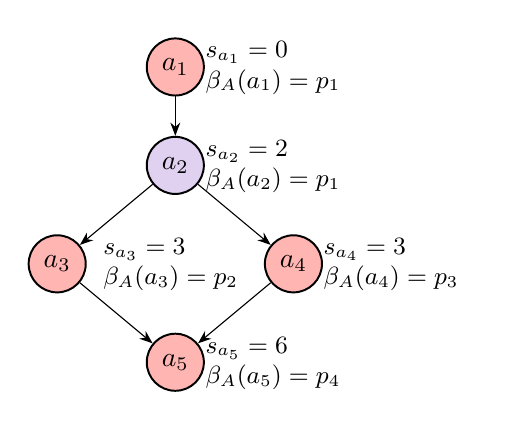
\begin{tikzpicture}
		\node[ActorStyle] (a1) {$\actor_1$};
		\node[ActorBroadcastStyle, below of=a1,yshift=-0.25cm] (a2) {$\actor_2$};
		\node[ActorStyle, below of=a2,yshift=-0.25cm, xshift=-1.5cm] (a3) {$\actor_3$};
		\node[ActorStyle, below of=a2,yshift=-0.25cm, xshift=1.5cm] (a4) {$\actor_4$};
		\node[ActorStyle, below of=a4,xshift=-1.5cm,yshift=-0.25cm] (a5) {$\actor_5$};
		
		\node[right of =a1,anchor=west,xshift=-0.95cm] {\small \begin{tabular}{l}$\startTime_{\actor_1} = 0$ \\ $\SetBindingsActors(\actor_1) = \core_1$ \end{tabular}};
		\node[right of =a2,anchor=west,xshift=-0.95cm] {\small \begin{tabular}{l}$\startTime_{\actor_2} = 2$ \\ $\SetBindingsActors(\actor_2) = \core_1$ \end{tabular}};
		\node[right of =a3,anchor=west,xshift=-0.75cm] {\small \begin{tabular}{l}$\startTime_{\actor_3} = 3$ \\ $\SetBindingsActors(\actor_3) = \core_2$ \end{tabular}};
		\node[right of =a4,anchor=west,xshift=-0.95cm] {\small \begin{tabular}{l}$\startTime_{\actor_4} = 3$ \\ $\SetBindingsActors(\actor_4) = \core_3$ \end{tabular}};
		\node[right of =a5,anchor=west,xshift=-0.95cm] {\small \begin{tabular}{l}$\startTime_{\actor_5} = 6$ \\ $\SetBindingsActors(\actor_5) = \core_4$ \end{tabular}};
		
		\draw[-{Stealth}] (a1) -> (a2);
		\draw[-{Stealth}] (a2) -> (a3);
		\draw[-{Stealth}] (a2) -> (a4);
		\draw[-{Stealth}] (a3) -> (a5);
		\draw[-{Stealth}] (a4) -> (a5);
    \end{tikzpicture}
  }
};

  \node[right of=graph1,xshift=-6.5cm,yshift=-0.0cm] (gantt) {
    \resizebox{160pt}{!}{
    \begin{tikzpicture}
      \scheduleNoComs
    \end{tikzpicture}
	}
  };
}

\newcommand*{\Lightning}[1][]{%
  \begin{scope}
    \filldraw[{#1}]
      (-.5, -.5) -- (.4, -.03) -- (-.1, .06) --
      (.5, .5) -- (-.4, .03) -- (.1, -.06) --
      cycle
      % side bearings
      (-.5 - .08, 0)
      (.5 + .08, 0)
    ;%
  \end{scope}
}


\newcommand{\ExampleHeuristic}{
\tikzfading[name=myfading, bottom color=transparent!0, top color=transparent!100]
\tikzfading[name=myfading2, left color=transparent!100, right color=transparent!0]

  \node (gantt1) at (0,0) {
    \resizebox{320pt}{!}{
    \begin{tikzpicture}
      \scheduleComsInit
    \end{tikzpicture}
	}
  };

  \node[right of=gantt1,xshift=10.3cm,yshift=0cm] (gantt2) {
    \resizebox{320pt}{!}{
    \begin{tikzpicture}
      \scheduleComsOne
    \end{tikzpicture}
	}
  };

  \draw [decorate,decoration={brace,amplitude=10pt,raise=4pt},yshift=0pt] (-4.1,2.9) -- (4.5,2.9) node [black,midway,xshift=0cm,yshift=1cm] {\Large Period $\Period=10$};
  \node at (0,-4.0) {\Large Time};

\node[right of=gantt1,xshift=-10.5cm,yshift=0cm](graph2) at (0,0) {
    \resizebox{210pt}{!}{
	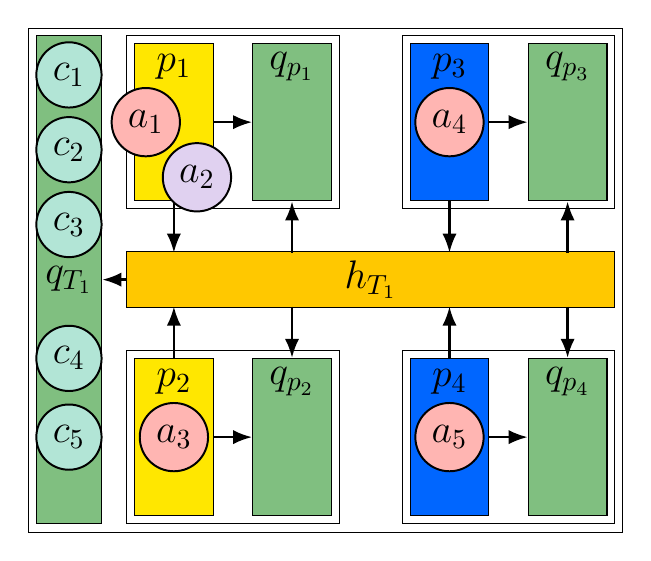
\begin{tikzpicture}
		\exBindingAllocation
    	\end{tikzpicture}
	}
};

  \draw [decorate,decoration={brace,amplitude=10pt,raise=4pt},yshift=0pt] (7.2,2.9) -- (15.7,2.90) node [black,midway,xshift=0cm,yshift=1cm] {\Large Period $\Period=10$};
  \node at (11.3,-4.0) {\Large Time};
}

\newcommand{\exBindingAllocation}{
\begin{scope}
    \node[CrossbarStyle,anchor=west] (h1) at (-0.1,-2) {\Large $\crossbar{1}$};
    \node[TileLocalMemStyle,anchor=west] (qh1) at (-1.25,-2) {\Large $\memory_{\tile_1}$};
    \draw[ArchitectureLinkStyle] (h1) -> (qh1);
    
    \node[CoreType1,anchor=west] (p1) at (0,0){};
    \node[yshift=0.7cm] (legp1) at (p1) {\Large $\core_1$};
    \node[LocalMemType, right of=p1, xshift=0.5cm] (qp1) {};
    \node[yshift=0.7cm] (legqp1) at (qp1) {\Large $\memory_{\core_1}$};
    \node[draw, minimum width=2.7cm, minimum height=2.2cm,anchor=west] (border1) at (-0.1,0){};
    \draw[ArchitectureLinkStyle] (p1) -> (qp1);
    \draw[ArchitectureLinkStyle] (p1.south) -> ($ (p1.south) + (0,-0.65) $);
    \draw[ArchitectureLinkStyle] ($ (qp1.south) + (0,-0.65) $) ->(qp1.south);

    \node[CoreType3,anchor=west] (p3) at (3.5,0){};
    \node[yshift=0.7cm] (legp3) at (p3) {\Large $\core_3$};
    \node[LocalMemType, right of=p3, xshift=0.5cm] (qp3) {};
    \node[yshift=0.7cm] (legqp3) at (qp3) {\Large $\memory_{\core_3}$};
    \node[draw, minimum width=2.7cm, minimum height=2.2cm,anchor=west] (border3) at (3.4,0) {};
    \draw[ArchitectureLinkStyle] (p3) -> (qp3);
    \draw[ArchitectureLinkStyle] (p3.south) -> ($ (p3.south) + (0,-0.65) $);
    \draw[ArchitectureLinkStyle] ($ (qp3.south) + (0,-0.65) $) ->(qp3.south);
 

    \node[CoreType1,anchor=west] (p2) at (0,-4) {};
    \node[yshift=0.7cm] (legp2) at (p2) {\Large $\core_2$};
    \node[LocalMemType, right of=p2, xshift=0.5cm] (qp2) {};
    \node[yshift=0.7cm] (legqp2) at (qp2) {\Large $\memory_{\core_2}$};
    \node[draw, minimum width=2.7cm, minimum height=2.2cm,anchor=west] (border2) at (-0.1,-4) {};
    \draw[ArchitectureLinkStyle] (p2) -> (qp2);
    \draw[ArchitectureLinkStyle] (p2.north) -> ($ (p2.north) + (0,0.65) $);
    \draw[ArchitectureLinkStyle] ($(qp2.north) + (0,0.65) $) ->(qp2.north);
    
    \node[CoreType3,anchor=west] (p4) at (3.5,-4) {};
    \node[yshift=0.7cm] (legp4) at (p4) {\Large $\core_4$};
    \node[LocalMemType, right of=p4, xshift=0.5cm] (qp4) {};
    \node[yshift=0.7cm] (legqp4) at (qp4) {\Large $\memory_{\core_4}$};
    \node[draw, minimum width=2.7cm, minimum height=2.2cm,anchor=west] (border4) at (3.4,-4) {};
    \draw[ArchitectureLinkStyle] (p4) -> (qp4);
    \draw[ArchitectureLinkStyle] (p4.north) -> ($ (p4.north) + (0,0.65) $);
    \draw[ArchitectureLinkStyle] ($(qp4.north) + (0,0.65) $) ->(qp4.north);

    \node[ActorStyle] (a1) at (0.15,0) {\Large $\actor_1$};
    \node[ActorBroadcastStyle] (a2) at (0.8,-0.7) {\Large $a_2$};
    \node[ActorStyle] (a3) at (p2) {\Large $\actor_3$};
    \node[ActorStyle] (a4) at (p3) {\Large $\actor_4$};
    \node[ActorStyle] (a5) at (p4) {\Large $\actor_5$};

    \node[ChannelStyle,yshift=2.6cm] (c1) at (qh1) {\Large $\channel_1$};
    \node[ChannelStyle,yshift=1.65cm] (c2) at (qh1) {\Large $\channel_2$};
    \node[ChannelStyle,yshift=0.7cm] (c3) at (qh1) {\Large $\channel_3$};
    \node[ChannelStyle,yshift=-1cm]  (c4) at (qh1) {\Large $\channel_4$};
    \node[ChannelStyle,yshift=-2cm](c5) at (qh1) {\Large $\channel_5$};

    \node[draw, minimum width=7.55cm, minimum height=6.4cm,anchor=north west] (border5) at (-1.35,1.2) {};

%    \node[below of =a3,text=red,yshift=0.4cm] {\large \bm{$\execTime=3$}};
%    \node[below of =a4,text=red,yshift=0.4cm] {\large \bm{$\execTime=3$}};
%    \node[below of =a5,text=red,yshift=0.4cm] {\large \bm{$\execTime=4$}};
%    \node[below of =a1,text=red,yshift=0.4cm,xshift=-0.2cm] {\large \bm{$\execTime=2$}};
%    \node[below of =a2,text=red,yshift=0.4cm,xshift=0.2cm] {\large \bm{$\execTime=1$}};
%    \node[below of =c5,text=red,yshift=0.4cm] {\large \bm{$\execTime=1$}};
\end{scope}
}


\newcommand{\scheduleComsInit}
{
\begin{scope}

	\begin{ganttchart}[ bar height=0.5, vrule/.style={line width=0.5mm, black,loosely dashed}, canvas/.style={ draw=none},
                vrule label font=\bfseries, link/.style={->, line width=1pt, black}  ]{1}{10} 
                \ganttbar[bar left shift=0.1, bar right shift=-1,bar top shift=0.4,bar/.style={draw=none}]
                {\huge $\Utilization_{\core_4}$}{0}{44}
                \\
                \ganttbar[bar left shift=0.1, bar right shift=-0.5,bar top shift=0.75,bar/.style={draw=none}]
                {\huge $\Utilization_{\core_3}$}{0}{30}
		\ganttCrossbarReadbarCore[CrossbarReadbarCore top shift=0.4,inline]{}{15}{16}
		\ganttActorbar[Actorbar top shift=0.4, inline,name=a4e2]{\Large$\actor_4$}{17}{20}
		\ganttActorbar[Actorbar top shift=0.4, inline,name=a4e1]{\Large$\actor_4$}{1}{2}
		\ganttCrossbarWritebarCore[CrossbarWritebarCore top shift=0.4,inline]{}{3}{4}
		\\
                \ganttbar[bar left shift=0.1, bar right shift=-0.5,bar top shift=1.2,bar/.style={draw=none}]
                {\huge $\Utilization_{\core_2}$}{0}{30}
		\ganttCrossbarReadbarCore[CrossbarReadbarCore top shift=0.8,inline]{}{15}{16}
		\ganttActorbar[Actorbar top shift=0.8, inline,name=a3e1]{\Large$\actor_3$}{17}{20}
                \ganttActorbar[Actorbar top shift=0.8,inline,name=a3e2]{\Large $\actor_3$ }{1}{2}
		\ganttCrossbarWritebarCore[CrossbarWritebarCore top shift=0.8,inline]{}{3}{4}
                \\
                \ganttbar[bar left shift=0.1, bar right shift=-0.5,bar top shift=1.6,bar/.style={draw=none}]
                {\huge $\Utilization_{\core_1}$}{0}{30}
                \ganttActorbar[Actorbar top shift=1.25,inline,name=a1e1]{\Large $\actor_1$}{1}{4}  
		\ganttCrossbarWritebarCore[CrossbarWritebarCore top shift=1.25,inline]{}{5}{6}
		\ganttCrossbarReadbarCore[CrossbarReadbarCore top shift=1.25,inline]{}{7}{8}
                \ganttBroadcastbar[Broadcastbar top shift=1.25,inline,name=a2e1]{\Large $\actor_2$ }{9}{10}
		\ganttCrossbarWritebarCore[CrossbarWritebarCore top shift=1.25,inline]{}{11}{14} 

                %\ganttActorbar[Actorbar top shift=1.25,inline,name=a1e2]{\Large $\actor_1$}{21}{22}   
 
                \\
                \ganttbar[bar left shift=0.1, bar right shift=0.5,bar top shift=2, bar/.style={draw=none}]{\huge $\Utilization_{\crossbar{1}}$}{0}{38}

                \ganttCrossbarWritebar[CrossbarWritebar top shift=1.7,inline,name=c1w1]{ $(\actor_1,\channel_1)$}{5}{6}             
                \ganttCrossbarReadbar[CrossbarReadbar   top shift=1.7,inline,name=c1r1]{ $(\channel_1,\actor_2)$}{7}{8}
                \ganttCrossbarWritebar[CrossbarWritebar top shift=1.7,inline,name=c2w1]{ $(\actor_2,\channel_2)$}{11}{12}            
                \ganttCrossbarWritebar[CrossbarWritebar top shift=1.7,inline,name=c3w1]{ $(\actor_2,\channel_3)$}{13}{14}             
                \ganttCrossbarReadbar[CrossbarReadbar   top shift=1.7,inline,name=c2r1]{ $(\channel_2,\actor_3)$}{15}{16}
                \ganttCrossbarWritebar[CrossbarWritebar top shift=1.7,inline,name=c4w1]{ $(\actor_3,\channel_4)$}{3}{4}            
                %\ganttCrossbarReadbar[CrossbarReadbar   top shift=1.7,inline,name=c3r1]{ $(\channel_3,\actor_4)$}{17}{18}	
		\\

		\ganttbar[bar/.style={draw=none}]{\huge }{0}{38}
       		\\
		\ganttbar[bar/.style={draw=none}]{\huge }{0}{38}      

        \draw[-Latex,line width=0.3mm,opacity=1] (a1e1) -| (c1w1);
        \draw[-Latex,line width=0.3mm,opacity=1] (c1r1) |- (a2e1);
        \draw[-Latex,line width=0.3mm,opacity=1] (a2e1) -| (c2w1);
        \draw[-Latex,line width=0.3mm,opacity=1] (a2e1) -| (c3w1);
        \draw[-Latex,line width=0.3mm,opacity=1] (c2r1) |- (a3e1);
        \draw[-Latex,line width=0.3mm,opacity=1,dashdotted] (a3e2) -| (c4w1);

        %\draw[-Latex,line width=0.3mm,opacity=0.5,dashdotted] (c3r1) |- (a4e2);


        \draw[-{Stealth},line width=0.3mm] (0,-7) -- (10.5,-7);
        \draw[-{Stealth},line width=0.3mm] (0,-7) -- (0,1);

	\ganttvrule{\Large}{20}

        \draw[line width=0.3mm,dashed] (1,-7) -- (1,-1);
        \draw[line width=0.3mm,dashed] (2,-7) -- (2,-1);

        \draw[line width=0.3mm,dashed] (7,-7) -- (7,-1);
        \draw[line width=0.3mm,dashed] (8,-7) -- (8,-1);

	\node at (2,-0.7) {\huge $\startTime_{(\actor_4,\channel_5)}$};

	\fill [ path fading=myfading2,fill=white] (10.3,0) rectangle (11.2,-7);
	 \foreach \x in {0,...,10}{
 		{\pgfmathtruncatemacro{\label}{(\x)}
		\node at (\x,-7.4) {\Large \label};}
		\draw[line width=0.4mm](\x,-6.8) -- (\x,-7.2);
	}
	\draw[line width=0.4mm](-0.15,-6.25) -- (0.2,-6.25);
	\draw[line width=0.4mm](-0.15,-4.8) -- (0.2,-4.8);
	\draw[line width=0.4mm](-0.15,-3.45) -- (0.2,-3.45);
	\draw[line width=0.4mm](-0.15,-2) -- (0.2,-2);
	\draw[line width=0.4mm](-0.15,-0.65) -- (0.2,-0.65);
%	\node at (9,0.5) {\Large $\Period=10$};
%	\node at (11,-6.5) {\Large Time};

	\node at (1.5,-2.25){
	   \resizebox{60pt}{!}{
	   
\begin{tikzpicture}
	     \Lightning[fill=yellow, line join=round, xscale=1.0]
	   \end{tikzpicture} }
	};

	\node at (7.5,-2.25){
	   \resizebox{60pt}{!}{
	   
\begin{tikzpicture}
	     \Lightning[fill=yellow, line join=round, xscale=1.0]
	   \end{tikzpicture} }
	};

    \end{ganttchart} 
\end{scope} 
}

\newcommand{\scheduleComsOne}
{
\begin{scope}

	\begin{ganttchart}[ bar height=0.5, vrule/.style={line width=0.5mm, black,loosely dashed}, canvas/.style={ draw=none},
                vrule label font=\bfseries, link/.style={->, line width=1pt, black}  ]{1}{10} 
                \ganttbar[bar left shift=0.1, bar right shift=-1,bar top shift=0.4,bar/.style={draw=none}]
                {\huge $\Utilization_{\core_4}$}{0}{44}
                \ganttActorbar[Actorbar top shift=0.0, inline,name=a5e1]{\Large $\actor_5$}{1}{8}
		\ganttCrossbarReadbarCore[CrossbarReadbarCore top shift=0,inline]{}{17}{20}
		%\ganttCrossbarReadbarCore[CrossbarReadbarCore top shift=0,inline]{}{1}{2}
                \\
                \ganttbar[bar left shift=0.1, bar right shift=-0.5,bar top shift=0.75,bar/.style={draw=none}]
                {\huge $\Utilization_{\core_3}$}{0}{30}
		\ganttCrossbarReadbarCore[CrossbarReadbarCore top shift=0.4,inline]{}{1}{2}
		%\ganttActorbar[Actorbar top shift=0.4, inline,name=a4e3]{\Large}{21}{22}
		%\ganttActorbar[Actorbar top shift=0.4, inline,name=a4e2]{\Large$\actor_4$}{19}{20}
		\ganttActorbar[Actorbar top shift=0.4, inline,name=a4e1]{\Large$\actor_4$}{3}{8}
		\ganttCrossbarWritebarCore[CrossbarWritebarCore top shift=0.4,inline]{}{9}{10}
		\\
                \ganttbar[bar left shift=0.1, bar right shift=-0.5,bar top shift=1.2,bar/.style={draw=none}]
                {\huge $\Utilization_{\core_2}$}{0}{30}
		\ganttCrossbarReadbarCore[CrossbarReadbarCore top shift=0.8,inline]{}{15}{16}
		\ganttActorbar[Actorbar top shift=0.8, inline,name=a3e1]{\Large$\actor_3$}{17}{20}
                \ganttActorbar[Actorbar top shift=0.8,inline,name=a3e2]{\Large $\actor_3$ }{1}{2}
		\ganttCrossbarWritebarCore[CrossbarWritebarCore top shift=0.8,inline]{}{3}{4}
                \\
                \ganttbar[bar left shift=0.1, bar right shift=-0.5,bar top shift=1.6,bar/.style={draw=none}]
                {\huge $\Utilization_{\core_1}$}{0}{30}
                \ganttActorbar[Actorbar top shift=1.25,inline,name=a1e1]{\Large $\actor_1$}{1}{4}  
                \ganttActorbar[Actorbar top shift=1.25,inline,name=a1e1]{\Large $\actor_1$}{1}{4}   
                \ganttBroadcastbar[Broadcastbar top shift=1.25,inline,name=a2e1]{\Large $\actor_2$ }{9}{10}       
		\ganttCrossbarWritebarCore[CrossbarWritebarCore top shift=1.25,inline]{}{11}{14} 
		\ganttCrossbarWritebarCore[CrossbarWritebarCore top shift=1.25,inline]{}{5}{6}
		\ganttCrossbarReadbarCore[CrossbarReadbarCore top shift=1.25,inline]{}{7}{8}
                \\
                \ganttbar[bar left shift=0.1, bar right shift=0.5,bar top shift=2, bar/.style={draw=none}]{\huge $\Utilization_{\crossbar{1}}$}{0}{38}

                \ganttCrossbarWritebar[CrossbarWritebar top shift=1.7,inline,name=c1w1]{ $(\actor_1,\channel_1)$}{5}{6}             
                \ganttCrossbarReadbar[CrossbarReadbar   top shift=1.7,inline,name=c1r1]{ $(\channel_1,\actor_2)$}{7}{8}
                \ganttCrossbarWritebar[CrossbarWritebar top shift=1.7,inline,name=c2w1]{ $(\actor_2,\channel_2)$}{11}{12}            
                \ganttCrossbarWritebar[CrossbarWritebar top shift=1.7,inline,name=c3w1]{ $(\actor_2,\channel_3)$}{13}{14}             
                \ganttCrossbarReadbar[CrossbarReadbar   top shift=1.7,inline,name=c2r1]{ $(\channel_2,\actor_3)$}{15}{16}
                \ganttCrossbarWritebar[CrossbarWritebar top shift=1.7,inline,name=c4w1]{ $(\actor_3,\channel_4)$}{3}{4}            
                \ganttCrossbarWritebar[CrossbarWritebar top shift=1.7,inline,name=c5w1]{ $(\actor_4,\channel_5)$}{9}{10}             
                \ganttCrossbarReadbar[CrossbarReadbar   top shift=1.7,inline,name=c4r1]{ $(\channel_4,\actor_5)$}{17}{18}
                \ganttCrossbarReadbar[CrossbarReadbar   top shift=1.7,inline,name=c5r1]{ $(\channel_5,\actor_5)$}{19}{20}
                \ganttCrossbarReadbar[CrossbarReadbar   top shift=1.7,inline,name=c3r1]{ $(\channel_3,\actor_4)$}{1}{2}

		\\

		\ganttbar[bar/.style={draw=none}]{\huge }{0}{38}
       		\\
		\ganttbar[bar/.style={draw=none}]{\huge }{0}{38}      

        \draw[-Latex,line width=0.3mm,opacity=1] (a1e1) -| (c1w1);
        \draw[-Latex,line width=0.3mm,opacity=1] (c1r1) |- (a2e1);
        \draw[-Latex,line width=0.3mm,opacity=1] (a2e1) -| (c2w1);
        \draw[-Latex,line width=0.3mm,opacity=1] (a2e1) -| (c3w1);
        \draw[-Latex,line width=0.3mm,opacity=1] (c2r1) |- (a3e1);
        \draw[-Latex,line width=0.3mm,opacity=1,dashdotted] (a3e2) -| (c4w1);
        \draw[-Latex,line width=0.3mm,opacity=1,dashdotted] (c3r1) |- (a4e1);
        \draw[-Latex,line width=0.3mm,opacity=1,dashdotted] (a4e1) -| (c5w1);

        \draw[-{Stealth},line width=0.3mm] (0,-7) -- (10.5,-7);
        \draw[-{Stealth},line width=0.3mm] (0,-7) -- (0,1);

	\ganttvrule{\Large}{20}
	\fill [ path fading=myfading2,fill=white] (10.3,0) rectangle (11.2,-7);

        \draw[-Latex,line width=0.3mm,opacity=1,dashdotted] (c4r1) |- (10,-0.5);
        \draw[-Latex,line width=0.3mm,opacity=1,dashdotted] (c5r1) |- (10,-0.5);

	 \foreach \x in {0,...,10}{
 		{\pgfmathtruncatemacro{\label}{(\x)}
		\node at (\x,-7.4) {\Large \label};}
		\draw[line width=0.4mm](\x,-6.8) -- (\x,-7.2);
	}
	\draw[line width=0.4mm](-0.15,-6.25) -- (0.2,-6.25);
	\draw[line width=0.4mm](-0.15,-4.8) -- (0.2,-4.8);
	\draw[line width=0.4mm](-0.15,-3.45) -- (0.2,-3.45);
	\draw[line width=0.4mm](-0.15,-2) -- (0.2,-2);
	\draw[line width=0.4mm](-0.15,-0.65) -- (0.2,-0.65);
%	\node at (9,0.5) {\Large $\Period=10$};
%	\node at (11,-6.5) {\Large Time};
    \end{ganttchart} 
\end{scope} 
}


\newcommand{\scheduleComsTwo}
{
\begin{scope}

	\begin{ganttchart}[ bar height=0.5, vrule/.style={line width=0.5mm, black,loosely dashed}, canvas/.style={ draw=none},
                vrule label font=\bfseries, link/.style={->, line width=1pt, black}  ]{1}{10} 
                \ganttbar[bar left shift=0.1, bar right shift=-1,bar top shift=0.4,bar/.style={draw=none}]
                {\huge $\core_4$}{0}{44}
                \ganttActorbar[Actorbar top shift=0.0, inline,name=a5e1]{\Large $\actor_5$}{1}{8}
		\ganttCrossbarReadbarCore[CrossbarReadbarCore top shift=0.0,inline]{}{17}{20}
                \ganttActorbar[Actorbar top shift=0.0, inline,name=a5e1]{\Large $\actor_5$}{21}{22}
                \\
                \ganttbar[bar left shift=0.1, bar right shift=-0.5,bar top shift=0.75,bar/.style={draw=none}]
                {\huge $\core_3$}{0}{30}
		\ganttCrossbarReadbarCore[CrossbarReadbarCore top shift=0.4,inline]{}{1}{2}
		\ganttActorbar[Actorbar top shift=0.4, inline,name=a4e1]{\Large$\actor_4$}{3}{8}
		\ganttCrossbarWritebarCore[CrossbarWritebarCore top shift=0.4,inline]{}{9}{10}
		\\
                \ganttbar[bar left shift=0.1, bar right shift=-0.5,bar top shift=1.2,bar/.style={draw=none}]
                {\huge $\core_2$}{0}{30}
		\ganttCrossbarReadbarCore[CrossbarReadbarCore top shift=0.8,inline]{}{15}{16}
		\ganttActorbar[Actorbar top shift=0.8, inline,name=a3e1]{\Large$\actor_3$}{17}{22}
                \ganttActorbar[Actorbar top shift=0.8,inline,name=a3e2]{\Large $\actor_3$ }{1}{2}
		\ganttCrossbarWritebarCore[CrossbarWritebarCore top shift=0.8,inline]{}{3}{4}
                \\
                \ganttbar[bar left shift=0.1, bar right shift=-0.5,bar top shift=1.6,bar/.style={draw=none}]
                {\huge $\core_1$}{0}{30}
                \ganttActorbar[Actorbar top shift=1.25,inline,name=a1e1]{\Large $\actor_1$}{1}{4}  
		\ganttCrossbarWritebarCore[CrossbarWritebarCore top shift=1.25,inline]{}{5}{6}
		\ganttCrossbarReadbarCore[CrossbarReadbarCore top shift=1.25,inline]{}{7}{8}
                \ganttBroadcastbar[Broadcastbar top shift=1.25,inline,name=a2e1]{\Large $\actor_2$ }{9}{10}
		\ganttCrossbarWritebarCore[CrossbarWritebarCore top shift=1.25,inline]{}{11}{14} 

                \ganttActorbar[Actorbar top shift=1.25,inline,name=a1e2]{\Large $\actor_1$}{21}{22}   
 
                \\
                \ganttbar[bar left shift=0.1, bar right shift=0.5,bar top shift=2, bar/.style={draw=none}]{\huge $\crossbar{1}$}{0}{38}

                \ganttCrossbarWritebar[CrossbarWritebar top shift=1.7,inline,name=c1w1]{ $(\actor_1,\channel_1)$}{5}{6}             
                \ganttCrossbarReadbar[CrossbarReadbar   top shift=1.7,inline,name=c1r1]{ $(\channel_1,\actor_2)$}{7}{8}
                \ganttCrossbarWritebar[CrossbarWritebar top shift=1.7,inline,name=c2w1]{ $(\actor_2,\channel_2)$}{11}{12}            
                \ganttCrossbarWritebar[CrossbarWritebar top shift=1.7,inline,name=c3w1]{ $(\actor_2,\channel_3)$}{13}{14}             
                \ganttCrossbarReadbar[CrossbarReadbar   top shift=1.7,inline,name=c2r1]{ $(\channel_2,\actor_3)$}{15}{16}
                \ganttCrossbarReadbar[CrossbarReadbar   top shift=1.7,inline,name=c3r1]{ $(\channel_3,\actor_4)$}{1}{2}
                \ganttCrossbarWritebar[CrossbarWritebar top shift=1.7,inline,name=c4w1]{ $(\actor_3,\channel_4)$}{3}{4}            
                \ganttCrossbarWritebar[CrossbarWritebar top shift=1.7,inline,name=c5w1]{ $(\actor_4,\channel_5)$}{9}{10}             
                \ganttCrossbarReadbar[CrossbarReadbar   top shift=1.7,inline,name=c4r1]{ $(\channel_4,\actor_5)$}{17}{18}
                \ganttCrossbarReadbar[CrossbarReadbar   top shift=1.7,inline,name=c5r1]{ $(\channel_5,\actor_5)$}{19}{20}

                \ganttCrossbarWritebar[CrossbarWritebar top shift=1.7,inline,name=c1w2]{ $(\actor_1,\channel_1)$}{21}{22}             

		
		\\

		\ganttbar[bar/.style={draw=none}]{\huge }{0}{38}
       		\\
		\ganttbar[bar/.style={draw=none}]{\huge }{0}{38}      

        \draw[-Latex,line width=0.3mm,opacity=1] (a1e1) -| (c1w1);
        \draw[-Latex,line width=0.3mm,opacity=1] (c1r1) |- (a2e1);
        \draw[-Latex,line width=0.3mm,opacity=1] (a2e1) -| (c2w1);
        \draw[-Latex,line width=0.3mm,opacity=1] (a2e1) -| (c3w1);
        \draw[-Latex,line width=0.3mm,opacity=1] (c2r1) |- (a3e1);
        \draw[-Latex,line width=0.3mm,opacity=0.5] (a3e2) -| (c4w1);
        \draw[-Latex,line width=0.3mm,opacity=0.5] (c3r1) |- (a4e1);
        \draw[-Latex,line width=0.3mm,opacity=0.5] (a4e1) -| (c5w1);

        \draw[-Latex,line width=0.3mm,opacity=0.5] (c4r1) |- (a5e1);
        \draw[-Latex,line width=0.3mm,opacity=0.5] (c5r1) |- (a5e1);

        \draw[-{Stealth},line width=0.3mm] (0,-7) -- (12,-7);
        \draw[-{Stealth},line width=0.3mm] (0,-7) -- (0,1);

	\ganttvrule{\Large}{20}
	\fill [ path fading=myfading2,fill=white] (10.3,0) rectangle (11.2,-7);
	 \foreach \x in {0,...,11}{
 		{\pgfmathtruncatemacro{\label}{(\x)}
		\node at (\x,-7.4) {\Large \label};}
		\draw[line width=0.4mm](\x,-6.8) -- (\x,-7.2);
	}
	\draw[line width=0.4mm](-0.15,-6.25) -- (0.2,-6.25);
	\draw[line width=0.4mm](-0.15,-4.8) -- (0.2,-4.8);
	\draw[line width=0.4mm](-0.15,-3.45) -- (0.2,-3.45);
	\draw[line width=0.4mm](-0.15,-2) -- (0.2,-2);
	\draw[line width=0.4mm](-0.15,-0.65) -- (0.2,-0.65);
	\node at (9,0.5) {\Large $\Period=10$};
	\node at (12,-6.5) {\Large Time};
    \end{ganttchart} 
\end{scope} 
}


\newcommand{\scheduleNoComs}
{
\begin{scope}

	\begin{ganttchart}[ bar height=0.5, vrule/.style={line width=0.5mm, black,loosely dashed}, canvas/.style={ draw=none},
                vrule label font=\bfseries, link/.style={->, line width=1pt, black}  ]{1}{10} 
                \ganttbar[bar left shift=0.1, bar right shift=-1,bar top shift=0.4,bar/.style={draw=none}]
                {\huge $\Utilization_{\core_4}$}{0}{44}
                \ganttActorbar[Actorbar top shift=0.0, inline,name=a5e2]{\Large $\actor_5$}{5}{8}
                \ganttActorbar[Actorbar top shift=0.0, inline,name=a5e1]{\Large $\actor_5$}{1}{4}
                \\
                \ganttbar[bar left shift=0.1, bar right shift=-0.5,bar top shift=0.75,bar/.style={draw=none}]
                {\huge $\Utilization_{\core_3}$}{0}{30}
		\ganttActorbar[Actorbar top shift=0.4, inline,name=a4e1]{\Large$\actor_4$}{7}{8}
		\ganttActorbar[Actorbar top shift=0.4, inline,name=a4e2]{\Large$\actor_4$}{1}{4}
		\\
                \ganttbar[bar left shift=0.1, bar right shift=-0.5,bar top shift=1.2,bar/.style={draw=none}]
                {\huge $\Utilization_{\core_2}$}{0}{30}
		\ganttActorbar[Actorbar top shift=0.8, inline,name=a3e1]{\Large$\actor_3$}{7}{8}
		\ganttActorbar[Actorbar top shift=0.8, inline,name=a3e2]{\Large$\actor_3$}{1}{4}

                \\
                \ganttbar[bar left shift=0.1, bar right shift=-0.5,bar top shift=1.6,bar/.style={draw=none}]
                {\huge $\Utilization_{\core_1}$}{0}{30}
                \ganttActorbar[Actorbar top shift=1.25,inline,name=a1e1]{\Large $\actor_1$}{1}{4}   
                \ganttBroadcastbar[Broadcastbar top shift=1.25,inline,name=a2e1]{\Large $\actor_2$ }{5}{6}        
                \\
                \ganttbar[bar left shift=0.1, bar right shift=0.5,bar top shift=2, bar/.style={draw=none}]{\huge $\crossbar{1}$}{0}{38}
		
		\\

		\ganttbar[bar/.style={draw=none}]{\huge }{0}{38}
       		\\
		\ganttbar[bar/.style={draw=none}]{\huge }{0}{38}      


        \draw[-{Stealth},line width=0.3mm] (0,-7) -- (5,-7);
        \draw[-{Stealth},line width=0.3mm] (0,-7) -- (0,1);

	%\ganttvrule{\Large}{0}
	\ganttvrule{\Large}{8}
	%\ganttvrule{\Large}{44}

	 \foreach \x in {0,...,4}{
 		{\pgfmathtruncatemacro{\label}{(\x)}
		\node at (\x,-7.4) {\Large \label};}
		\draw[line width=0.4mm](\x,-6.8) -- (\x,-7.2);
	}

        \draw[-Latex,line width=0.3mm,opacity=1] (a2e1) |- (a3e1);
        \draw[-Latex,line width=0.3mm,opacity=1] (a2e1) |- (a4e1);

        \draw[-Latex,line width=0.3mm,opacity=1] (a3e2) -| ($(a5e2.south)+(-0.75,0)$);
        \draw[-Latex,line width=0.3mm,opacity=1] (a4e2) -| ($(a5e2.south)+(-0.75,0)$);

	\draw[line width=0.4mm](-0.15,-6.25) -- (0.2,-6.25);
	\draw[line width=0.4mm](-0.15,-4.8) -- (0.2,-4.8);
	\draw[line width=0.4mm](-0.15,-3.45) -- (0.2,-3.45);
	\draw[line width=0.4mm](-0.15,-2) -- (0.2,-2);
	\draw[line width=0.4mm](-0.15,-0.65) -- (0.2,-0.65);
	\node at (3,0.5) {\Large $\Period=4$};
	\node at (5,-6.5) {\Large Time};

    \end{ganttchart} 

\end{scope} 
}



\newcommand{\scheduleComsAll}
{
\tikzfading[name=myfading2, left color=transparent!100, right color=transparent!0]
\begin{scope}
	\begin{ganttchart}[ bar height=0.5, vrule/.style={line width=0.5mm, black,loosely dashed}, canvas/.style={ draw=none},
                vrule label font=\bfseries, link/.style={->, line width=1pt, black}  ]{1}{10} 
                \ganttbar[bar left shift=0.1, bar right shift=-1,bar top shift=0.4,bar/.style={draw=none}]
                {\huge $\core_4$}{0}{44}
                \ganttActorbar[Actorbar top shift=0.0, inline,name=a5e1]{\Large $\actor_5$}{3}{10}
		\ganttCrossbarReadbarCore[CrossbarReadbarCore top shift=0,inline]{}{19}{22}
		\ganttCrossbarReadbarCore[CrossbarReadbarCore top shift=0,inline]{}{1}{2}
                \\
                \ganttbar[bar left shift=0.1, bar right shift=-0.5,bar top shift=0.75,bar/.style={draw=none}]
                {\huge $\core_3$}{0}{30}
		\ganttCrossbarReadbarCore[CrossbarReadbarCore top shift=0.4,inline]{}{17}{18}
		\ganttActorbar[Actorbar top shift=0.4, inline,name=a4e3]{\Large}{21}{22}
		\ganttActorbar[Actorbar top shift=0.4, inline,name=a4e2]{\Large$\actor_4$}{19}{20}
		\ganttActorbar[Actorbar top shift=0.4, inline,name=a4e1]{\Large$\actor_4$}{1}{4}
		\ganttCrossbarWritebarCore[CrossbarWritebarCore top shift=0.4,inline]{}{9}{10}
		\\
                \ganttbar[bar left shift=0.1, bar right shift=-0.5,bar top shift=1.2,bar/.style={draw=none}]
                {\huge $\core_2$}{0}{30}
		\ganttCrossbarReadbarCore[CrossbarReadbarCore top shift=0.8,inline]{}{15}{16}
		\ganttActorbar[Actorbar top shift=0.8, inline,name=a3e1]{\Large$\actor_3$}{17}{22}
                \ganttActorbar[Actorbar top shift=0.8,inline,name=a3e2]{\Large $\actor_3$ }{1}{2}
		\ganttCrossbarWritebarCore[CrossbarWritebarCore top shift=0.8,inline]{}{3}{4}
                \\
                \ganttbar[bar left shift=0.1, bar right shift=-0.5,bar top shift=1.6,bar/.style={draw=none}]
                {\huge $\core_1$}{0}{30}
                \ganttActorbar[Actorbar top shift=1.25,inline,name=a1e1]{\Large $\actor_1$}{1}{4}  
                \ganttActorbar[Actorbar top shift=1.25,inline,name=a1e1]{\Large $\actor_1$}{1}{4}   
                \ganttBroadcastbar[Broadcastbar top shift=1.25,inline,name=a2e1]{\Large $\actor_2$ }{9}{10}       
                \ganttActorbar[Actorbar top shift=1.25,inline,name=a1e2]{\Large $\actor_1$}{21}{22}   
		\ganttCrossbarWritebarCore[CrossbarWritebarCore top shift=1.25,inline]{}{11}{14} 
		\ganttCrossbarWritebarCore[CrossbarWritebarCore top shift=1.25,inline]{}{5}{6}
		\ganttCrossbarReadbarCore[CrossbarReadbarCore top shift=1.25,inline]{}{7}{8}
                \\
                \ganttbar[bar left shift=0.1, bar right shift=0.5,bar top shift=2, bar/.style={draw=none}]{\huge $\crossbar{1}$}{0}{38}

                \ganttCrossbarWritebar[CrossbarWritebar top shift=1.7,inline,name=c1w1]{ $(\actor_1,\channel_1)$}{5}{6}             
                \ganttCrossbarReadbar[CrossbarReadbar   top shift=1.7,inline,name=c1r1]{ $(\channel_1,\actor_2)$}{7}{8}
                \ganttCrossbarWritebar[CrossbarWritebar top shift=1.7,inline,name=c2w1]{ $(\actor_2,\channel_2)$}{11}{12}            
                \ganttCrossbarWritebar[CrossbarWritebar top shift=1.7,inline,name=c3w1]{ $(\actor_2,\channel_3)$}{13}{14}             
                \ganttCrossbarReadbar[CrossbarReadbar   top shift=1.7,inline,name=c2r1]{ $(\channel_2,\actor_3)$}{15}{16}
                \ganttCrossbarReadbar[CrossbarReadbar   top shift=1.7,inline,name=c3r1]{ $(\channel_3,\actor_4)$}{17}{18}
                \ganttCrossbarWritebar[CrossbarWritebar top shift=1.7,inline,name=c4w1]{ $(\actor_3,\channel_4)$}{3}{4}            
                \ganttCrossbarWritebar[CrossbarWritebar top shift=1.7,inline,name=c5w1]{ $(\actor_4,\channel_5)$}{9}{10}             
                \ganttCrossbarReadbar[CrossbarReadbar   top shift=1.7,inline,name=c4r1]{ $(\channel_4,\actor_5)$}{19}{20}
                \ganttCrossbarReadbar[CrossbarReadbar   top shift=1.7,inline,name=c5r1]{ $(\channel_5,\actor_5)$}{1}{2}
                \ganttCrossbarReadbar[CrossbarReadbar   top shift=1.7,inline]{}{21}{22}
		\\

		\ganttbar[bar/.style={draw=none}]{\huge }{0}{38}
       		\\
		\ganttbar[bar/.style={draw=none}]{\huge }{0}{38}      

        \draw[-Latex,line width=0.3mm,opacity=1] (a1e1) -| (c1w1);
        \draw[-Latex,line width=0.3mm,opacity=1] (c1r1) |- (a2e1);
        \draw[-Latex,line width=0.3mm,opacity=1] (a2e1) -| (c2w1);
        \draw[-Latex,line width=0.3mm,opacity=1] (a2e1) -| (c3w1);
        \draw[-Latex,line width=0.3mm,opacity=1] (c2r1) |- (a3e1);
        \draw[-Latex,line width=0.3mm,opacity=0.5] (a3e2) -| (c4w1);
        \draw[-Latex,line width=0.3mm,opacity=0.5] (c3r1) |- (a4e2);
        \draw[-Latex,line width=0.3mm,opacity=0.5] (a4e1) -| (c5w1);

        \draw[-Latex,line width=0.3mm,opacity=0.5] (c5r1) |- (a5e1);

        \draw[-{Stealth},line width=0.3mm] (0,-7) -- (12,-7);
        \draw[-{Stealth},line width=0.3mm] (0,-7) -- (0,1);

	\ganttvrule{\Large}{20}
	\fill [ path fading=myfading2,fill=white] (10.3,0) rectangle (11.2,-7);

        \draw[-Latex,line width=0.3mm,opacity=0.5] (c4r1) |- (11,-0.5);

	 \foreach \x in {0,...,11}{
 		{\pgfmathtruncatemacro{\label}{(\x)}
		\node at (\x,-7.4) {\Large \label};}
		\draw[line width=0.4mm](\x,-6.8) -- (\x,-7.2);
	}
	\draw[line width=0.4mm](-0.15,-6.25) -- (0.2,-6.25);
	\draw[line width=0.4mm](-0.15,-4.8) -- (0.2,-4.8);
	\draw[line width=0.4mm](-0.15,-3.45) -- (0.2,-3.45);
	\draw[line width=0.4mm](-0.15,-2) -- (0.2,-2);
	\draw[line width=0.4mm](-0.15,-0.65) -- (0.2,-0.65);
	\node at (9,0.5) {\Large $\Period=10$};
	\node at (12,-6.5) {\Large Time};
    \end{ganttchart} 
\end{scope} 
}

% channels mapped to tile local memory of reader
\newcommand{\scheduleComsChannelsReadersAll}
{
\tikzfading[name=myfading2, left color=transparent!100, right color=transparent!0]
\begin{scope}
	\begin{ganttchart}[ bar height=0.5, vrule/.style={line width=0.5mm, black,loosely dashed}, canvas/.style={ draw=none},
                vrule label font=\bfseries, link/.style={->, line width=1pt, black}  ]{1}{10} 
                \ganttbar[bar left shift=0.1, bar right shift=-1,bar top shift=0.4,bar/.style={draw=none}]
                {\huge $\core_4$}{0}{44}
                \ganttActorbar[Actorbar top shift=0.0, inline,name=a5e1]{\Large $\actor_5$}{7}{14}
                \ganttActorbar[Actorbar top shift=0.0, inline,name=a5e2]{\Large}{21}{22}
		%\ganttCrossbarReadbarCore[CrossbarReadbarCore top shift=0,inline]{}{19}{22}
		%\ganttCrossbarReadbarCore[CrossbarReadbarCore top shift=0,inline]{}{1}{2}
                \\
                \ganttbar[bar left shift=0.1, bar right shift=-0.5,bar top shift=0.75,bar/.style={draw=none}]
                {\huge $\core_3$}{0}{30}
		%\ganttCrossbarReadbarCore[CrossbarReadbarCore top shift=0.4,inline]{}{17}{18}
		\ganttActorbar[Actorbar top shift=0.4, inline,name=a4e2]{\Large$\actor_4$}{11}{16}
		\ganttActorbar[Actorbar top shift=0.4, inline,name=a4e1]{\Large$\actor_4$}{1}{2}
		\ganttCrossbarWritebarCore[CrossbarWritebarCore top shift=0.4,inline]{}{5}{6}
		\ganttCrossbarWritebarCore[CrossbarWritebarCore top shift=0.4,inline]{}{19}{20}
		\\
                \ganttbar[bar left shift=0.1, bar right shift=-0.5,bar top shift=1.2,bar/.style={draw=none}]
                {\huge $\core_2$}{0}{30}
%		\ganttCrossbarReadbarCore[CrossbarReadbarCore top shift=0.8,inline]{}{15}{16}
		\ganttActorbar[Actorbar top shift=0.8, inline,name=a3e1]{\Large$\actor_3$}{11}{16}
                \ganttActorbar[Actorbar top shift=0.8,inline,name=a3e2]{\Large $\actor_3$ }{1}{2}
		\ganttCrossbarWritebarCore[CrossbarWritebarCore top shift=0.8,inline]{}{3}{4}
		\ganttCrossbarWritebarCore[CrossbarWritebarCore top shift=0.8,inline]{}{17}{18}
                \\
                \ganttbar[bar left shift=0.1, bar right shift=-0.5,bar top shift=1.6,bar/.style={draw=none}]
                {\huge $\core_1$}{0}{30}
                \ganttActorbar[Actorbar top shift=1.25,inline,name=a1e1]{\Large $\actor_1$}{1}{4}  
                \ganttBroadcastbar[Broadcastbar top shift=1.25,inline,name=a2e1]{\Large $\actor_2$ }{5}{6}       
		\ganttCrossbarWritebarCore[CrossbarWritebarCore top shift=1.25,inline]{}{7}{10} 

                \ganttActorbar[Actorbar top shift=1.25,inline,name=a1e2]{\Large $\actor_1$}{15}{18}  
                \ganttBroadcastbar[Broadcastbar top shift=1.25,inline,name=a2e2]{\Large $\actor_2$ }{19}{20}       
		\ganttCrossbarWritebarCore[CrossbarWritebarCore top shift=1.25,inline]{}{21}{22} 


                \\
                \ganttbar[bar left shift=0.1, bar right shift=0.5,bar top shift=2, bar/.style={draw=none}]{\huge $\crossbar{1}$}{0}{38}

                \ganttCrossbarWritebar[CrossbarWritebar top shift=1.7,inline,name=c4w1]{ $(\actor_3,\channel_4)$}{3}{4}            
                \ganttCrossbarWritebar[CrossbarWritebar top shift=1.7,inline,name=c5w1]{ $(\actor_4,\channel_5)$}{5}{6}             
                \ganttCrossbarWritebar[CrossbarWritebar top shift=1.7,inline,name=c2w1]{ $(\actor_2,\channel_2)$}{7}{8}            
                \ganttCrossbarWritebar[CrossbarWritebar top shift=1.7,inline,name=c3w1]{ $(\actor_2,\channel_3)$}{9}{10}             

                \ganttCrossbarWritebar[CrossbarWritebar top shift=1.7,inline,name=c4w2]{ $(\actor_3,\channel_4)$}{17}{18}            
                \ganttCrossbarWritebar[CrossbarWritebar top shift=1.7,inline,name=c5w2]{ $(\actor_4,\channel_5)$}{19}{20}             
                \ganttCrossbarWritebar[CrossbarWritebar top shift=1.7,inline,name=c2w2]{ $(\actor_2,\channel_2)$}{21}{22}            

		\\

		\ganttbar[bar/.style={draw=none}]{\huge }{0}{38}
       		\\
		\ganttbar[bar/.style={draw=none}]{\huge }{0}{38}      

        \draw[-Latex,line width=0.3mm,opacity=1] (a2e1) -| (c2w1);
        \draw[-Latex,line width=0.3mm,opacity=1] (a2e1) -| (c3w1);
        \draw[-Latex,line width=0.3mm,opacity=0.5] (a3e2) -| (c4w1);
        \draw[-Latex,line width=0.3mm,opacity=0.5] (a4e1) -| (c5w1);

        \draw[-Latex,line width=0.3mm,opacity=1] (a2e2) -| (c2w2);
        \draw[-Latex,line width=0.3mm,opacity=0.5] (a3e1) -| (c4w2);
        \draw[-Latex,line width=0.3mm,opacity=0.5] (a4e2) -| (c5w2);

        \draw[-{Stealth},line width=0.3mm] (0,-7) -- (12,-7);
        \draw[-{Stealth},line width=0.3mm] (0,-7) -- (0,1);

	\ganttvrule{\Large}{14}
	\fill [ path fading=myfading2,fill=white] (10.3,0) rectangle (11.2,-7);

%        \draw[-Latex,line width=0.3mm,opacity=0.5] (c4r1) |- (11,-0.5);

	 \foreach \x in {0,...,11}{
 		{\pgfmathtruncatemacro{\label}{(\x)}
		\node at (\x,-7.4) {\Large \label};}
		\draw[line width=0.4mm](\x,-6.8) -- (\x,-7.2);
	}
	\draw[line width=0.4mm](-0.15,-6.25) -- (0.2,-6.25);
	\draw[line width=0.4mm](-0.15,-4.8) -- (0.2,-4.8);
	\draw[line width=0.4mm](-0.15,-3.45) -- (0.2,-3.45);
	\draw[line width=0.4mm](-0.15,-2) -- (0.2,-2);
	\draw[line width=0.4mm](-0.15,-0.65) -- (0.2,-0.65);
	\node at (6,0.5) {\Large $\Period=7$};
	\node at (12,-6.5) {\Large Time};
    \end{ganttchart} 
\end{scope} 
}


% channels mapped to tile local memory of writer
\newcommand{\scheduleComsChannelsWritersAll}
{
\tikzfading[name=myfading2, left color=transparent!100, right color=transparent!0]
\begin{scope}
	\begin{ganttchart}[ bar height=0.5, vrule/.style={line width=0.5mm, black,loosely dashed}, canvas/.style={ draw=none},
                vrule label font=\bfseries, link/.style={->, line width=1pt, black}  ]{1}{10} 
                \ganttbar[bar left shift=0.1, bar right shift=-1,bar top shift=0.4,bar/.style={draw=none}]
                {\huge $\core_4$}{0}{44}
                \ganttActorbar[Actorbar top shift=0.0, inline,name=a5e1]{\Large $\actor_5$}{3}{10}
                \ganttActorbar[Actorbar top shift=0.0, inline,name=a5e2]{\Large $\actor_5$ }{15}{22}
                \ganttCrossbarReadbarCore[CrossbarReadbarCore top shift=0,inline]{}{1}{2}
		\ganttCrossbarReadbarCore[CrossbarReadbarCore top shift=0,inline]{}{11}{14}
                \\
                \ganttbar[bar left shift=0.1, bar right shift=-0.5,bar top shift=0.75,bar/.style={draw=none}]
                {\huge $\core_3$}{0}{30}
		\ganttActorbar[Actorbar top shift=0.4, inline,name=a4e2]{\Large$\actor_4$}{11}{16}
		\ganttActorbar[Actorbar top shift=0.4, inline,name=a4e1]{\Large$\actor_4$}{1}{4}
		\ganttCrossbarReadbarCore[CrossbarReadbarCore top shift=0.4,inline]{}{9}{10}
                \ganttCrossbarReadbarCore[CrossbarReadbarCore top shift=0.8,inline]{}{21}{22}
		\\
                \ganttbar[bar left shift=0.1, bar right shift=-0.5,bar top shift=1.2,bar/.style={draw=none}]
                {\huge $\core_2$}{0}{30}
		\ganttActorbar[Actorbar top shift=0.8, inline,name=a3e1]{\Large$\actor_3$}{1}{2}
                \ganttActorbar[Actorbar top shift=0.8, inline,name=a3e2]{\Large$\actor_3$}{9}{14}
		\ganttCrossbarReadbarCore[CrossbarReadbarCore top shift=0.8,inline]{}{7}{8}
		\ganttCrossbarReadbarCore[CrossbarReadbarCore top shift=0.8,inline]{}{19}{20}
                \ganttActorbar[Actorbar top shift=0.8, inline,name=a3e3]{}{21}{22}
                \\
                \ganttbar[bar left shift=0.1, bar right shift=-0.5,bar top shift=1.6,bar/.style={draw=none}]
                {\huge $\core_1$}{0}{30}
                \ganttActorbar[Actorbar top shift=1.25,inline,name=a1e1]{\Large $\actor_1$}{1}{4}  
                \ganttBroadcastbar[Broadcastbar top shift=1.25,inline,name=a2e1]{\Large $\actor_2$ }{5}{6}       
                \ganttActorbar[Actorbar top shift=1.25,inline,name=a1e2]{\Large $\actor_1$}{13}{16}  
                \ganttBroadcastbar[Broadcastbar top shift=1.25,inline,name=a2e2]{\Large $\actor_2$ }{17}{18}       
                \\
                \ganttbar[bar left shift=0.1, bar right shift=0.5,bar top shift=2, bar/.style={draw=none}]{\huge $\crossbar{1}$}{0}{38}

                \ganttCrossbarReadbar[CrossbarReadbar top shift=1.7,inline,name=c5r1]{ $(\channel_5,\actor_5)$}{1}{2}           


                \ganttCrossbarReadbar[CrossbarReadbar top shift=1.7,inline,name=c2r1]{ $(\channel_2,\actor_3)$}{7}{8}            
                \ganttCrossbarReadbar[CrossbarReadbar top shift=1.7,inline,name=c3r1]{ $(\channel_3,\actor_4)$}{9}{10}             
                \ganttCrossbarReadbar[CrossbarReadbar top shift=1.7,inline,name=c4r2]{ $(\channel_4,\actor_5)$}{11}{12}            
                \ganttCrossbarReadbar[CrossbarReadbar top shift=1.7,inline,name=c5r2]{ $(\channel_5,\actor_5)$}{13}{14}           


                \ganttCrossbarReadbar[CrossbarReadbar top shift=1.7,inline,name=c2r2]{ $(\channel_2,\actor_3)$}{19}{20}            
                \ganttCrossbarReadbar[CrossbarReadbar top shift=1.7,inline,name=c4r3]{ $(\channel_4,\actor_5)$}{21}{22}            
		\\

		\ganttbar[bar/.style={draw=none}]{\huge }{0}{38}
       		\\
		\ganttbar[bar/.style={draw=none}]{\huge }{0}{38}      

        \draw[-Latex,line width=0.3mm,opacity=0.5] (c5r1) |- (a5e1);

        \draw[-Latex,line width=0.3mm,opacity=1] (c2r1) |- (a3e2);
        \draw[-Latex,line width=0.3mm,opacity=0.5] (c3r1) |- (a4e2);

        \draw[-Latex,line width=0.3mm,opacity=0.5] (c5r2) |- (a5e2);

        \draw[-Latex,line width=0.3mm,opacity=0.5] (c4r2) |- (a5e2);
        \draw[-Latex,line width=0.3mm,opacity=0.5] (c2r2) |- (a3e3);
        \draw[-Latex,line width=0.3mm,opacity=0.5] (c4r3) |- (11.25,-2.25);




        \draw[-{Stealth},line width=0.3mm] (0,-7) -- (12,-7);
        \draw[-{Stealth},line width=0.3mm] (0,-7) -- (0,1);

	\ganttvrule{\Large}{12}
	\fill [ path fading=myfading2,fill=white] (10.3,0) rectangle (11.2,-7);

%        \draw[-Latex,line width=0.3mm,opacity=0.5] (c4r1) |- (11,-0.5);

	 \foreach \x in {0,...,11}{
 		{\pgfmathtruncatemacro{\label}{(\x)}
		\node at (\x,-7.4) {\Large \label};}
		\draw[line width=0.4mm](\x,-6.8) -- (\x,-7.2);
	}
	\draw[line width=0.4mm](-0.15,-6.25) -- (0.2,-6.25);
	\draw[line width=0.4mm](-0.15,-4.8) -- (0.2,-4.8);
	\draw[line width=0.4mm](-0.15,-3.45) -- (0.2,-3.45);
	\draw[line width=0.4mm](-0.15,-2) -- (0.2,-2);
	\draw[line width=0.4mm](-0.15,-0.65) -- (0.2,-0.65);
	\node at (5,0.5) {\Large $\Period=6$};
	\node at (12,-6.5) {\Large Time};
    \end{ganttchart} 
\end{scope} 
}



\newcommand{\scheduleMRB}
{
\tikzfading[name=myfading2, left color=transparent!100, right color=transparent!0]
\begin{scope}
	\begin{ganttchart}[ bar height=0.5, vrule/.style={line width=0.5mm, black,loosely dashed}, canvas/.style={ draw=none},
                vrule label font=\bfseries, link/.style={->, line width=1pt, black}  ]{1}{10} 
                \ganttbar[bar left shift=0.1, bar right shift=-1,bar top shift=0.4,bar/.style={draw=none}]
                {\huge $\core_4$}{0}{44}
                \ganttActorbar[Actorbar top shift=0.0, inline,name=a5e1]{\Large $\actor_5$}{1}{8}
                \ganttActorbar[Actorbar top shift=0.0, inline,name=a5e2]{\Large $\actor_5$}{15}{22}
		\ganttCrossbarReadbarCore[CrossbarReadbarCore top shift=0,inline]{}{11}{14}
                \\
                \ganttbar[bar left shift=0.1, bar right shift=-0.5,bar top shift=0.75,bar/.style={draw=none}]
                {\huge $\core_3$}{0}{30}
		\ganttActorbar[Actorbar top shift=0.4, inline,name=a4e1]{\Large$\actor_4$}{1}{2}
		\ganttCrossbarWritebarCore[CrossbarWritebarCore top shift=0.4,inline]{}{3}{4}
		\ganttActorbar[Actorbar top shift=0.4, inline,name=a4e2]{\Large$\actor_4$}{11}{16}
		\ganttCrossbarReadbarCore[CrossbarReadbarCore top shift=0.4,inline]{}{9}{10}
		\ganttCrossbarWritebarCore[CrossbarWritebarCore top shift=0.4,inline]{}{17}{18}
		\\
                \ganttbar[bar left shift=0.1, bar right shift=-0.5,bar top shift=1.2,bar/.style={draw=none}]
                {\huge $\core_2$}{0}{30}
		\ganttCrossbarWritebarCore[CrossbarWritebarCore top shift=0.8,inline]{}{1}{2}	
		\ganttActorbar[Actorbar top shift=0.8, inline,name=a3e1]{\Large$\actor_3$}{9}{14}
		\ganttCrossbarWritebarCore[CrossbarWritebarCore top shift=0.8,inline]{}{15}{16}
		\ganttCrossbarReadbarCore[CrossbarReadbarCore top shift=0.8,inline]{}{7}{8}
		\ganttCrossbarReadbarCore[CrossbarReadbarCore top shift=0.8,inline]{}{21}{22}
                \\
                \ganttbar[bar left shift=0.1, bar right shift=-0.5,bar top shift=1.6,bar/.style={draw=none}]
                {\huge $\core_1$}{0}{30}
                \ganttActorbar[Actorbar top shift=1.25,inline,name=a1e1]{\Large $\actor_1$}{1}{4}  
		\ganttCrossbarWritebarCore[CrossbarWritebarCore top shift=1.25,inline]{}{5}{6} 

                \ganttActorbar[Actorbar top shift=1.25,inline,name=a1e2]{\Large $\actor_1$}{15}{18} 
		\ganttCrossbarWritebarCore[CrossbarWritebarCore top shift=1.25,inline]{}{19}{20} 

                \\
                \ganttbar[bar left shift=0.1, bar right shift=0.5,bar top shift=2, bar/.style={draw=none}]{\huge $\crossbar{1}$}{0}{38}

                \ganttCrossbarWritebar[CrossbarWritebar top shift=1.7,inline,name=c4w1]{ $(\actor_3,\channel_4)$}{1}{2}            
                \ganttCrossbarWritebar[CrossbarWritebar top shift=1.7,inline,name=c5w1]{ $(\actor_4,\channel_5)$}{3}{4}           
                \ganttCrossbarWritebar[CrossbarWritebar top shift=1.7,inline,name=mrbw1]{\footnotesize $\channel_{\{1,2,3\}}$}{5}{6}            
                \ganttCrossbarReadbar[CrossbarReadbar top shift=1.7,inline,name=mrbr1]{ \footnotesize $\channel_{\{1,2,3\}}$}{7}{8}            
                \ganttCrossbarReadbar[CrossbarReadbar top shift=1.7,inline,name=mrbr2]{ \footnotesize $\channel_{\{1,2,3\}}$}{9}{10}             
                \ganttCrossbarReadbar[CrossbarReadbar top shift=1.7,inline,name=c4r1]{ $(\channel_4,\actor_5)$}{11}{12}            
                \ganttCrossbarReadbar[CrossbarReadbar top shift=1.7,inline,name=c5r1]{ $(\channel_5,\actor_5)$}{13}{14}           

                \ganttCrossbarWritebar[CrossbarWritebar top shift=1.7,inline,name=c4w2]{ $(\actor_3,\channel_4)$}{15}{16}            
                \ganttCrossbarWritebar[CrossbarWritebar top shift=1.7,inline,name=c5w2]{ $(\actor_4,\channel_5)$}{17}{18}           
                \ganttCrossbarWritebar[CrossbarWritebar top shift=1.7,inline,name=mrbw2]{\footnotesize $\channel_{\{1,2,3\}}$}{19}{20}            
                \ganttCrossbarReadbar[CrossbarReadbar top shift=1.7,inline,name=mrbr4]{ \footnotesize $\channel_{\{1,2,3\}}$}{21}{22}            

		\\

		\ganttbar[bar/.style={draw=none}]{\huge }{0}{38}
       		\\
		\ganttbar[bar/.style={draw=none}]{\huge }{0}{38}      

        \draw[-Latex,line width=0.3mm,opacity=0.5] (a4e1) -| (c5w1);
        \draw[-Latex,line width=0.3mm,opacity=1] (a1e1) -| (mrbw1);
        \draw[-Latex,line width=0.3mm,opacity=1.0] (mrbr1) |- (a3e1);
        \draw[-Latex,line width=0.3mm,opacity=0.5] (mrbr2) |- (a4e2);
        \draw[-Latex,line width=0.3mm,opacity=0.5] (c4r1) |- (a5e2);
        \draw[-Latex,line width=0.3mm,opacity=0.5] (c5r1) |- (a5e2);

        \draw[-Latex,line width=0.3mm,opacity=0.5] (a3e1) -| (c4w2);
        \draw[-Latex,line width=0.3mm,opacity=0.5] (a4e2) -| (c5w2);
        \draw[-Latex,line width=0.3mm,opacity=1] (a1e2) -| (mrbw2);

        \draw[-{Stealth},line width=0.3mm] (0,-7) -- (12,-7);
        \draw[-{Stealth},line width=0.3mm] (0,-7) -- (0,1);

	\ganttvrule{\Large}{14}
	\fill [ path fading=myfading2,fill=white] (10.3,0) rectangle (11.2,-7);

%        \draw[-Latex,line width=0.3mm,opacity=0.5] (c4r1) |- (11,-0.5);

	 \foreach \x in {0,...,11}{
 		{\pgfmathtruncatemacro{\label}{(\x)}
		\node at (\x,-7.4) {\Large \label};}
		\draw[line width=0.4mm](\x,-6.8) -- (\x,-7.2);
	}
	\draw[line width=0.4mm](-0.15,-6.25) -- (0.2,-6.25);
	\draw[line width=0.4mm](-0.15,-4.8) -- (0.2,-4.8);
	\draw[line width=0.4mm](-0.15,-3.45) -- (0.2,-3.45);
	\draw[line width=0.4mm](-0.15,-2) -- (0.2,-2);
	\draw[line width=0.4mm](-0.15,-0.65) -- (0.2,-0.65);
	\node at (6,0.5) {\Large $\Period=7$};
	\node at (12,-6.5) {\Large Time};
    \end{ganttchart} 
\end{scope} 
}


\newcommand{\scheduleMRBOnlyWrites}
{
\tikzfading[name=myfading2, left color=transparent!100, right color=transparent!0]
\begin{scope}
	\begin{ganttchart}[ bar height=0.5, vrule/.style={line width=0.5mm, black,loosely dashed}, canvas/.style={ draw=none},
                vrule label font=\bfseries, link/.style={->, line width=1pt, black}  ]{1}{10} 
                \ganttbar[bar left shift=0.1, bar right shift=-1,bar top shift=0.4,bar/.style={draw=none}]
                {\huge $\core_4$}{0}{44}
                \ganttActorbar[Actorbar top shift=0.0, inline,name=a5e1]{}{1}{2}
                \ganttActorbar[Actorbar top shift=0.0, inline,name=a5e1]{\Large $\actor_5$}{5}{12}
                \ganttActorbar[Actorbar top shift=0.0, inline,name=a5e2]{\Large $\actor_5$}{15}{22}
                \\
                \ganttbar[bar left shift=0.1, bar right shift=-0.5,bar top shift=0.75,bar/.style={draw=none}]
                {\huge $\core_3$}{0}{30}
		\ganttCrossbarReadbarCore[CrossbarReadbarCore top shift=0.4,inline]{}{1}{2}
		\ganttActorbar[Actorbar top shift=0.4, inline,name=a4e1]{\Large$\actor_4$}{3}{8}
		\ganttCrossbarWritebarCore[CrossbarWritebarCore top shift=0.4,inline]{}{9}{10}
		\ganttCrossbarReadbarCore[CrossbarReadbarCore top shift=0.4,inline]{}{11}{12}
		\ganttActorbar[Actorbar top shift=0.4, inline,name=a4e2]{\Large$\actor_4$}{13}{18}
		\ganttCrossbarWritebarCore[CrossbarWritebarCore top shift=0.4,inline]{}{19}{20}
		\ganttCrossbarReadbarCore[CrossbarReadbarCore top shift=0.4,inline]{}{21}{22}
		\\
                \ganttbar[bar left shift=0.1, bar right shift=-0.5,bar top shift=1.2,bar/.style={draw=none}]
                {\huge $\core_2$}{0}{30}
		\ganttActorbar[Actorbar top shift=0.8, inline,name=a3e1]{\Large$\actor_3$}{1}{2}
		\ganttCrossbarWritebarCore[CrossbarWritebarCore top shift=0.8,inline]{}{3}{4}	
		\ganttActorbar[Actorbar top shift=0.8, inline,name=a3e2]{\Large$\actor_3$}{7}{12}
		\ganttCrossbarWritebarCore[CrossbarWritebarCore top shift=0.8,inline]{}{13}{14}
		\ganttActorbar[Actorbar top shift=0.8, inline,name=a3e3]{\Large$\actor_3$}{17}{22}
                \\
                \ganttbar[bar left shift=0.1, bar right shift=-0.5,bar top shift=1.6,bar/.style={draw=none}]
                {\huge $\core_1$}{0}{30}
                \ganttActorbar[Actorbar top shift=1.25,inline,name=a1e1]{\Large $\actor_1$}{1}{4}  
		\ganttCrossbarWritebarCore[CrossbarWritebarCore top shift=1.25,inline]{}{5}{6} 

                \ganttActorbar[Actorbar top shift=1.25,inline,name=a1e2]{\Large $\actor_1$}{11}{14} 
		\ganttCrossbarWritebarCore[CrossbarWritebarCore top shift=1.25,inline]{}{15}{16}

                \ganttActorbar[Actorbar top shift=1.25,inline,name=a1e3]{}{21}{22} 

                \\
                \ganttbar[bar left shift=0.1, bar right shift=0.5,bar top shift=2, bar/.style={draw=none}]{\huge $\crossbar{1}$}{0}{38}


                \ganttCrossbarReadbar[CrossbarReadbar top shift=1.7,inline,name=mrbr1]{ \footnotesize $\channel_{\{1,2,3\}}$}{1}{2}            
                \ganttCrossbarWritebar[CrossbarWritebar top shift=1.7,inline,name=c4w1]{ $(\actor_3,\channel_4)$}{3}{4}            
                \ganttCrossbarWritebar[CrossbarWritebar top shift=1.7,inline,name=c1w1]{ $(\actor_1,\channel_1)$}{5}{6}           
                \ganttCrossbarWritebar[CrossbarWritebar top shift=1.7,inline,name=c5w1]{ $(\actor_4,\channel_5)$}{9}{10}           

                \ganttCrossbarReadbar[CrossbarReadbar top shift=1.7,inline,name=mrbr2]{ \footnotesize $\channel_{\{1,2,3\}}$}{11}{12}            
                \ganttCrossbarWritebar[CrossbarWritebar top shift=1.7,inline,name=c4w2]{ $(\actor_3,\channel_4)$}{13}{14}            
                \ganttCrossbarWritebar[CrossbarWritebar top shift=1.7,inline,name=c1w2]{ $(\actor_1,\channel_1)$}{15}{16}           
                \ganttCrossbarWritebar[CrossbarWritebar top shift=1.7,inline,name=c5w2]{ $(\actor_4,\channel_5)$}{19}{20}           

                \ganttCrossbarReadbar[CrossbarReadbar top shift=1.7,inline,name=mrbr3]{ \footnotesize $\channel_{\{1,2,3\}}$}{21}{22}

		\\

		\ganttbar[bar/.style={draw=none}]{\huge }{0}{38}
       		\\
		\ganttbar[bar/.style={draw=none}]{\huge }{0}{38}      


        \draw[-Latex,line width=0.3mm,opacity=0.5] (mrbr1) |- (a4e1);
        \draw[-Latex,line width=0.3mm,opacity=0.5] (a3e1) -|  (c4w1);
        \draw[-Latex,line width=0.3mm,opacity=1.0] (a1e1) -| (c1w1);
        \draw[-Latex,line width=0.3mm,opacity=0.5] (a4e1) -| (c5w1);

        \draw[-Latex,line width=0.3mm,opacity=0.5] (mrbr2) |- (a4e2);
        \draw[-Latex,line width=0.3mm,opacity=0.5] (a3e2) -|  (c4w2);
        \draw[-Latex,line width=0.3mm,opacity=1.0] (a1e2) -| (c1w2);
        \draw[-Latex,line width=0.3mm,opacity=0.5] (a4e2) -| (c5w2);




        \draw[-{Stealth},line width=0.3mm] (0,-7) -- (12,-7);
        \draw[-{Stealth},line width=0.3mm] (0,-7) -- (0,1);

	\ganttvrule{\Large}{10}
	\ganttvrule{\Large}{20}

	\fill [ path fading=myfading2,fill=white] (10.3,0) rectangle (11.2,-7);

	 \foreach \x in {0,...,11}{
 		{\pgfmathtruncatemacro{\label}{(\x)}
		\node at (\x,-7.4) {\Large \label};}
		\draw[line width=0.4mm](\x,-6.8) -- (\x,-7.2);
	}
	\draw[line width=0.4mm](-0.15,-6.25) -- (0.2,-6.25);
	\draw[line width=0.4mm](-0.15,-4.8) -- (0.2,-4.8);
	\draw[line width=0.4mm](-0.15,-3.45) -- (0.2,-3.45);
	\draw[line width=0.4mm](-0.15,-2) -- (0.2,-2);
	\draw[line width=0.4mm](-0.15,-0.65) -- (0.2,-0.65);
	\node at (4,0.5) {\Large $\Period=5$};
	\node at (12,-6.5) {\Large Time};
    \end{ganttchart} 
\end{scope} 
}

\newcommand{\scheduleMRBOnlyReads}
{
\tikzfading[name=myfading2, left color=transparent!100, right color=transparent!0]
\begin{scope}
	\begin{ganttchart}[ bar height=0.5, vrule/.style={line width=0.5mm, black,loosely dashed}, canvas/.style={ draw=none},
                vrule label font=\bfseries, link/.style={->, line width=1pt, black}  ]{1}{10} 
                \ganttbar[bar left shift=0.1, bar right shift=-1,bar top shift=0.4,bar/.style={draw=none}]
                {\huge $\core_4$}{0}{44}
		\ganttCrossbarReadbarCore[CrossbarReadbarCore top shift=0.0,inline]{}{1}{4}
		\ganttCrossbarReadbarCore[CrossbarReadbarCore top shift=0.0,inline]{}{13}{16}
                \ganttActorbar[Actorbar top shift=0.0, inline,name=a5e1]{\Large $\actor_5$}{5}{12}
                \ganttActorbar[Actorbar top shift=0.0, inline,name=a5e2]{\Large $\actor_5$}{17}{22}
                \\
                \ganttbar[bar left shift=0.1, bar right shift=-0.5,bar top shift=0.75,bar/.style={draw=none}]
                {\huge $\core_3$}{0}{30}
		\ganttActorbar[Actorbar top shift=0.4, inline,name=a4e1]{\Large$\actor_4$}{1}{2}
		\ganttActorbar[Actorbar top shift=0.4, inline,name=a4e2]{\Large$\actor_4$}{9}{14}
		\ganttCrossbarReadbarCore[CrossbarReadbarCore top shift=0.4,inline]{}{7}{8}
		\ganttCrossbarReadbarCore[CrossbarReadbarCore top shift=0.4,inline]{}{19}{20}
		\ganttActorbar[Actorbar top shift=0.4, inline,name=a4e3]{}{21}{22}
		\\
                \ganttbar[bar left shift=0.1, bar right shift=-0.5,bar top shift=1.2,bar/.style={draw=none}]
                {\huge $\core_2$}{0}{30}
		\ganttCrossbarReadbarCore[CrossbarReadbarCore top shift=0.8,inline]{}{5}{6}
		\ganttCrossbarReadbarCore[CrossbarReadbarCore top shift=0.8,inline]{}{17}{18}	
		\ganttActorbar[Actorbar top shift=0.8, inline,name=a3e1]{\Large$\actor_3$}{7}{12}
		\ganttActorbar[Actorbar top shift=0.8, inline,name=a3e2]{\Large$\actor_3$}{19}{22}
                \\
                \ganttbar[bar left shift=0.1, bar right shift=-0.5,bar top shift=1.6,bar/.style={draw=none}]
                {\huge $\core_1$}{0}{30}
                \ganttActorbar[Actorbar top shift=1.25,inline,name=a1e1]{\Large $\actor_1$}{1}{4}  

                \ganttActorbar[Actorbar top shift=1.25,inline,name=a1e2]{\Large $\actor_1$}{13}{16} 


                \\
                \ganttbar[bar left shift=0.1, bar right shift=0.5,bar top shift=2, bar/.style={draw=none}]{\huge $\crossbar{1}$}{0}{38}

                \ganttCrossbarReadbar[CrossbarReadbar top shift=1.7,inline,name=c4r1]{ $(\channel_4,\actor_5)$}{1}{2}            
                \ganttCrossbarReadbar[CrossbarReadbar top shift=1.7,inline,name=c5r1]{ $(\channel_5,\actor_5)$}{3}{4}            
                \ganttCrossbarReadbar[CrossbarReadbar top shift=1.7,inline,name=mrbr1]{\footnotesize $\channel_{\{1,2,3\}}$}{5}{6}            
                \ganttCrossbarReadbar[CrossbarReadbar top shift=1.7,inline,name=mrbr2]{\footnotesize $\channel_{\{1,2,3\}}$}{7}{8}            

                \ganttCrossbarReadbar[CrossbarReadbar top shift=1.7,inline,name=c4r2]{ $(\channel_4,\actor_5)$}{13}{14}            
                \ganttCrossbarReadbar[CrossbarReadbar top shift=1.7,inline,name=c5r2]{ $(\channel_5,\actor_5)$}{15}{16}            
                \ganttCrossbarReadbar[CrossbarReadbar top shift=1.7,inline,name=mrbr3]{\footnotesize $\channel_{\{1,2,3\}}$}{17}{18}            
                \ganttCrossbarReadbar[CrossbarReadbar top shift=1.7,inline,name=mrbr4]{\footnotesize $\channel_{\{1,2,3\}}$}{19}{20}            

		\\

		\ganttbar[bar/.style={draw=none}]{\huge }{0}{38}
       		\\
		\ganttbar[bar/.style={draw=none}]{\huge }{0}{38}      

        \draw[-Latex,line width=0.3mm,opacity=0.5] (c4r1) |- (a5e1);
        \draw[-Latex,line width=0.3mm,opacity=0.5] (c5r1) |- (a5e1);
        \draw[-Latex,line width=0.3mm,opacity=0.5] (mrbr1) |- (a3e1);
        \draw[-Latex,line width=0.3mm,opacity=0.5] (mrbr2) |- (a4e2);

        \draw[-Latex,line width=0.3mm,opacity=0.5] (c4r2) |- (a5e2);
        \draw[-Latex,line width=0.3mm,opacity=0.5] (c5r2) |- (a5e2);
        \draw[-Latex,line width=0.3mm,opacity=0.5] (mrbr3) |- (a3e2);
        \draw[-Latex,line width=0.3mm,opacity=0.5] (mrbr4) |- (a4e3);

        \draw[-{Stealth},line width=0.3mm] (0,-7) -- (12,-7);
        \draw[-{Stealth},line width=0.3mm] (0,-7) -- (0,1);

	\ganttvrule{\Large}{12}
	\fill [ path fading=myfading2,fill=white] (10.3,0) rectangle (11.2,-7);

%        \draw[-Latex,line width=0.3mm,opacity=0.5] (c4r1) |- (11,-0.5);

	 \foreach \x in {0,...,11}{
 		{\pgfmathtruncatemacro{\label}{(\x)}
		\node at (\x,-7.4) {\Large \label};}
		\draw[line width=0.4mm](\x,-6.8) -- (\x,-7.2);
	}
	\draw[line width=0.4mm](-0.15,-6.25) -- (0.2,-6.25);
	\draw[line width=0.4mm](-0.15,-4.8) -- (0.2,-4.8);
	\draw[line width=0.4mm](-0.15,-3.45) -- (0.2,-3.45);
	\draw[line width=0.4mm](-0.15,-2) -- (0.2,-2);
	\draw[line width=0.4mm](-0.15,-0.65) -- (0.2,-0.65);
	\node at (5,0.5) {\Large $\Period=6$};
	\node at (12,-6.5) {\Large Time};
    \end{ganttchart} 
\end{scope} 
}


\newcommand{\comparisonCores}{
  \begin{groupplot}[group style={
                      group name=Combinatorial,
                      group size= 3 by 2,
                      xlabels at=edge bottom,
                      ylabels at=edge left,
                      vertical sep=1.6cm,
                    },
                    height=3.8cm,width=7.0cm,
                    ylabel={\large Utilization [\%]},
                    legend style = {at={(0.0,-0.35)}},
                    legend columns             = 3,
                    xlabel={\large Number of Generations},
                    legend columns=3,
                    xmode=normal,
                    ybar,
                    ymin =0,
                    ymax =100,
                    enlarge x limits=0.3,
                    xtick={0,1,2},
                    xticklabels={$\Reference$,$\MergingAlways$,$\MergingExplore$}
                    ]
                     
    \nextgroupplot[title={\large Sobel}]
      \addplot[CoreOneBar] table[x index=0,y index=1,col sep=tab]{csv/cores-utilization/ModuloScheduling-BindingsDSE-Sobel-Sequential-ALL.csv};
      \addplot[CoreTwoBar] table[x index=0,y index=2,col sep=tab]{csv/cores-utilization/ModuloScheduling-BindingsDSE-Sobel-Sequential-ALL.csv};
      \addplot[CoreThreeBar] table[x index=0,y index=3,col sep=tab]{csv/cores-utilization/ModuloScheduling-BindingsDSE-Sobel-Sequential-ALL.csv};
                 
    \nextgroupplot[title={\large Sobel split 4}]
      \addplot[CoreOneBar] table[x index=0,y index=1,col sep=tab]{csv/cores-utilization/ModuloScheduling-BindingsDSE-Sobel-Parallel-ALL.csv};
      \addplot[CoreTwoBar] table[x index=0,y index=2,col sep=tab]{csv/cores-utilization/ModuloScheduling-BindingsDSE-Sobel-Parallel-ALL.csv};
      \addplot[CoreThreeBar] table[x index=0,y index=3,col sep=tab]{csv/cores-utilization/ModuloScheduling-BindingsDSE-Sobel-Parallel-ALL.csv};

    \nextgroupplot[title={\large Multicamera}]
      \addlegendimage{CoreOneBar}
      \addlegendentry{\large cores of type $\coretype_1$}
      \addlegendimage{CoreTwoBar}
      \addlegendentry{\large cores of type $\coretype_2$}
      \addlegendimage{CoreThreeBar}
      \addlegendentry{\large cores of type $\coretype_3$}

      \addplot[CoreOneBar] table[x index=0,y index=1,col sep=tab]{csv/cores-utilization/ModuloScheduling-BindingsDSE-Multicamera-ALL.csv};
      \addplot[CoreTwoBar] table[x index=0,y index=2,col sep=tab]{csv/cores-utilization/ModuloScheduling-BindingsDSE-Multicamera-ALL.csv};
      \addplot[CoreThreeBar] table[x index=0,y index=3,col sep=tab]{csv/cores-utilization/ModuloScheduling-BindingsDSE-Multicamera-ALL.csv};

\end{groupplot}
}

\newcommand{\comparisonInterconnect}{
\pgfplotsset{every tick label/.append style={font=\large}}

  \begin{groupplot}[group style={
                      group name=Combinatorial,
                      group size= 3 by 2,
                      xlabels at=edge bottom,
                      ylabels at=edge left,
                      vertical sep=1.6cm,
                    },
                    height=4cm,width=9.0cm,
                    ylabel={\Large Utilization [\%]},
                    legend style = {at={(0.75,-0.35)}},
                    legend columns             = 5,
                    xlabel={\Large Number of Generations},
                    xmode=normal,
                    ybar,
                    ymin =0,
                    ymax =100,
                    enlarge x limits=0.3,
                    xtick={0,1,2},
                    xticklabels={\Large $\Reference$, \Large $\MergingAlways$, \Large $\MergingExplore$}
                    ]
                     
    \nextgroupplot[title={\Large Sobel}]
      \addplot[LocalMemBar] table[x index=0,y index=11,col sep=tab]{csv/cores-utilization/ModuloScheduling-BindingsDSE-Sobel-Sequential-ALL.csv};
      \addplot[TileMemBar] table[x index=0,y index=8,col sep=tab]{csv/cores-utilization/ModuloScheduling-BindingsDSE-Sobel-Sequential-ALL.csv};
      \addplot[GlobalMemBar] table[x index=0,y index=10,col sep=tab]{csv/cores-utilization/ModuloScheduling-BindingsDSE-Sobel-Sequential-ALL.csv};
      \addplot[CrossbarBar] table[x index=0,y expr={(\thisrowno{4}+\thisrowno{5}+\thisrowno{6})/3 }  ,col sep=tab]{csv/cores-utilization/ModuloScheduling-BindingsDSE-Sobel-Sequential-ALL.csv};
      \addplot[NOCBar] table[x index=0,y index=9,col sep=tab]{csv/cores-utilization/ModuloScheduling-BindingsDSE-Sobel-Sequential-ALL.csv};
                 
    \nextgroupplot[title={\Large Sobel split 4}]
      \addplot[LocalMemBar] table[x index=0,y index=11,col sep=tab]{csv/cores-utilization/ModuloScheduling-BindingsDSE-Sobel-Parallel-ALL.csv};
      \addplot[TileMemBar] table[x index=0,y index=8,col sep=tab]{csv/cores-utilization/ModuloScheduling-BindingsDSE-Sobel-Parallel-ALL.csv};
      \addplot[GlobalMemBar] table[x index=0,y index=10,col sep=tab]{csv/cores-utilization/ModuloScheduling-BindingsDSE-Sobel-Parallel-ALL.csv};
      \addplot[CrossbarBar] table[x index=0,y expr={(\thisrowno{4}+\thisrowno{5}+\thisrowno{6})/3 }  ,col sep=tab]{csv/cores-utilization/ModuloScheduling-BindingsDSE-Sobel-Parallel-ALL.csv};
      \addplot[NOCBar] table[x index=0,y index=9,col sep=tab]{csv/cores-utilization/ModuloScheduling-BindingsDSE-Sobel-Parallel-ALL.csv};

    \nextgroupplot[title={\Large Multicamera}]
      \addlegendimage{LocalMemBar}
      \addlegendentry{\Large core local memories ($\memory_\core$)}
      \addlegendimage{TileMemBar}
      \addlegendentry{\Large tile local memories ($\memory_\tile$)}
      \addlegendimage{GlobalMemBar}
      \addlegendentry{\Large global memory ($\GlobalMemory$)}
      \addlegendimage{CrossbarBar}
      \addlegendentry{\Large crossbars ($\crossbar{}$)}
      \addlegendimage{NOCBar}
      \addlegendentry{\Large NoC ($\NoC$)}

      \addplot[LocalMemBar] table[x index=0,y index=11,col sep=tab]{csv/cores-utilization/ModuloScheduling-BindingsDSE-Multicamera-ALL.csv};
      \addplot[TileMemBar] table[x index=0,y index=8,col sep=tab]{csv/cores-utilization/ModuloScheduling-BindingsDSE-Multicamera-ALL.csv};
      \addplot[GlobalMemBar] table[x index=0,y index=10,col sep=tab]{csv/cores-utilization/ModuloScheduling-BindingsDSE-Multicamera-ALL.csv};
      \addplot[CrossbarBar] table[x index=0,y expr={(\thisrowno{4}+\thisrowno{5}+\thisrowno{6}+\thisrowno{7})/4 }  ,col sep=tab]{csv/cores-utilization/ModuloScheduling-BindingsDSE-Multicamera-ALL.csv};
      \addplot[NOCBar] table[x index=0,y index=9,col sep=tab]{csv/cores-utilization/ModuloScheduling-BindingsDSE-Multicamera-ALL.csv};

\end{groupplot}
}


\newcommand{\HypervolumeLastIteration}{
\begin{groupplot}[ 
                    group style={
                    group name                 = LastIterHyper,
                    group size                 = 4 by 2,
                    xlabels at                 = edge bottom,
                    ylabels at                 = edge left,
		    vertical sep=1.7cm,
                    },
      width=7.5cm,%
      height=3.9cm,%
      ybar=1pt,%
%      bar width=0.3cm,%
      enlarge x limits=0.3,% horizontal spacing
      %symbolic x coords={10,20,30},%
      xtick={10,20,30},
      xticklabels={Sobel, Sobel$_4$, Multicamera},%
      every node near coord/.append style={rotate=90, anchor=west,font=\scriptsize },
      nodes near coords,
      nodes near coords align={vertical},
      ylabel={hypervolume},%
      x tick label style={font=\small},
      y tick label style={font=\small},
      legend style={at={(0.975,-0.25)},draw=none,fill=none,legend columns=3},
      legend cell align=left,
      ymax=1.2,
      ytick={0.2,0.4,0.6,0.8,1},
      yticklabels={0.2,0.4,0.6,0.8,1},
      axis lines*=left,
%      clip=false,
      ]

  \nextgroupplot[title=Hypervolume of last generation, bar width=0.2cm  ]
    \addlegendimage{draw=black, fill=amaranth!30}
    \addlegendentry{\footnotesize $\Reference^{ILP}$}
    \addlegendimage{draw=black, fill=amaranth!90}
    \addlegendentry{\footnotesize $\MergingAlways^{ILP}$}
    \addlegendimage{draw=black, fill=carmine}
    \addlegendentry{\footnotesize $\MergingExplore^{ILP}$}
    \addlegendimage{draw=black, fill=babyblue}
    \addlegendentry{\footnotesize $\Reference^{\fHeuristic}$}
    \addlegendimage{draw=black, fill=azureBlue}
    \addlegendentry{\footnotesize $\MergingAlways^{\fHeuristic}$}
    \addlegendimage{draw=black, fill=blue}
    \addlegendentry{\footnotesize $\MergingExplore^{\fHeuristic}$}

    \addplot[draw=black, fill=amaranth!30] table[y index=1, x index=0,col sep=tab]{csv/gains/ILP-hypervolumes-last-generation.csv};
    \addplot[draw=black, fill=amaranth!90] table[y index=2, x index=0,col sep=tab]{csv/gains/ILP-hypervolumes-last-generation.csv};
    \addplot[draw=black, fill=carmine] table[y index=3, x index=0,col sep=tab]{csv/gains/ILP-hypervolumes-last-generation.csv};
    \addplot[draw=black, fill=babyblue] table[y index=1, x index=0,col sep=tab]{csv/gains/Heuristic-hypervolumes-last-generation.csv};
    \addplot[draw=black, fill=azureBlue] table[y index=2, x index=0,col sep=tab]{csv/gains/Heuristic-hypervolumes-last-generation.csv};
    \addplot[draw=black, fill=blue] table[y index=3, x index=0,col sep=tab]{csv/gains/Heuristic-hypervolumes-last-generation.csv};
    
\end{groupplot}
}


\newcommand{\GainHypervolumeLastIteration}{
\begin{groupplot}[ 
                    group style={
                    group name                 = LastIterHyper,
                    group size                 = 4 by 2,
                    xlabels at                 = edge bottom,
                    ylabels at                 = edge left,
		    vertical sep=1.7cm,
                    },
      width=6.2cm,%
      height=4.3cm,%
      ybar=1pt,%
%      bar width=0.3cm,%
      enlarge x limits=0.3,% horizontal spacing
      %symbolic x coords={10,20,30},%
      xtick={10,20,30},
      xticklabels={Sobel, Sobel$_4$, Multicamera},%
%      xticklabel style={align=center},%
%      xtick=data,%
%      xtick pos=left,
%      ytick pos=left,
%      y tick style={transparent},% hide x tick marks
%      ymin=0,%
%      ymax=7,%
      ylabel={gain [$\%$]},%
      x tick label style={font=\small},
      y tick label style={font=\small},
%      ymajorgrids,
%      ytick={0,2,4,6,8,10,12,14,16},
      legend style={at={(1.1,-0.25)},draw=none,fill=none,legend columns=2},
      legend cell align=left,
      ymax=230,
%      restrict y to domain*=0:110,
      axis lines*=left,
%      clip=false,
      ytick={50,100,150,200},
      yticklabels={50,100,150,200},
      every node near coord/.append style={rotate=90, anchor=west,font=\scriptsize },
      nodes near coords, 
      nodes near coords align={vertical},
      ]

  \nextgroupplot[title=Hypervolume gains of the last generation, bar width=0.2cm  ]
    \addlegendimage{draw=amaranth!90, fill=amaranth!90}
    \addlegendentry{\footnotesize $\text{gain}(\MergingAlways^{ILP})$}
    \addlegendimage{draw=carmine, fill=carmine}
    \addlegendentry{\footnotesize $\text{gain}(\MergingExplore^{ILP})$}
    \addlegendimage{draw=azureBlue, fill=azureBlue}
    \addlegendentry{\footnotesize $\text{gain}(\MergingAlways^{\fHeuristic})$}
    \addlegendimage{draw=blue, fill=blue}
    \addlegendentry{\footnotesize $\text{gain}(\MergingExplore^{\fHeuristic})$}

    \addplot[draw=amaranth!90, fill=amaranth!90] table[y index=1, x index=0,col sep=tab]{csv/gains/ILP-gains-last-generation.csv};
    \addplot[draw=carmine, fill=carmine] table[y index=2, x index=0,col sep=tab]{csv/gains/ILP-gains-last-generation.csv};
    \addplot[draw=azureBlue, fill=azureBlue] table[y index=1, x index=0,col sep=tab]{csv/gains/Heuristic-gains-last-generation.csv};
    \addplot[draw=blue, fill=blue] table[y index=2, x index=0,col sep=tab]{csv/gains/Heuristic-gains-last-generation.csv};

\end{groupplot}
}

%\renewcommand{\figurename}{Fig.}
%\Crefname{algorithm}{Alg.}{Algs.}


\usepackage{textcomp}
\def\BibTeX{{\rm B\kern-.05em{\sc i\kern-.025em b}\kern-.08em
    T\kern-.1667em\lower.7ex\hbox{E}\kern-.125emX}}

\DeclareCaptionFont{blue}{\color{accessblue}}
\DeclareCaptionLabelSeparator{dot}{. }
\captionsetup{labelsep=dot,labelfont={blue,bf,sf,footnotesize}}

\let\mod\undefined % get rid of old \mod
\DeclareMathOperator{\mod}{mod}
\renewcommand{\baselinestretch}{0.988}
\begin{document}
\bstctlcite{IEEEexample:BSTcontrol}
\history{{\textcolor{white}{Date of publication xxxx 00, 0000, date of current version xxxx 00, 0000.}}}
%\doi{10.1109/ACCESS.2023.0322000}
\doi{}
\title{Exploring Multi-Reader Buffers and Channel Placement during Dataflow Network Mapping to Heterogeneous Many-core Systems
}
\author{\uppercase{Martín Letras}~\orcidlink{0000-0002-1429-8982},
\uppercase{Joachim Falk}~\orcidlink{0009-0006-0834-3237}, and \uppercase{J{\"u}rgen Teich}~\orcidlink{0000-0001-6285-5862} \IEEEmembership{Fellow, IEEE}}
\address{Friedrich-Alexander-Universität Erlangen-Nürnberg (FAU), Erlangen, Germany (e-mail:\{martin.letras, joachim.falk, juergen.teich\}@fau.de)}
\tfootnote{\revised{This work has been partially funded by the Deutsche Forschungsgemeinschaft (DFG, German Research Foundation) under project grants 502213043 and 530178246.}}
%\tfootnote{This paragraph of the first footnote will contain support
%information, including sponsor and financial support acknowledgment. For
%example, ``This work was supported in part by the U.S. Department of
%Commerce under Grant BS123456.''}
\markboth
%{Letras, Falk, and Teich \headeretal: Preparation of Papers for IEEE TRANSACTIONS and JOURNALS}
{Letras, Falk, and Teich}
{Letras, Falk, and Teich}
\corresp{Corresponding author: Martin Letras (e-mail: martin.letras@fau.de).}
\def\thevol{1}
%to hide logos
%\def\headerlogo{\raisebox{-2pt}{}}
%\def\headerlogoall{\raisebox{-2pt}{}}
\begin{abstract}
This paper presents an approach for reducing the memory requirements \revised{of periodically executed} dataflow applications, while \revised{minimizing the period} when deployed on a many-core target.
Often, implementations of dataflow applications suffer from data duplication if identical data has to be processed by multiple actors.
In fact, multi-cast (also called fork) actors can produce huge memory overheads when storing and communicating copies of the same data.
As a remedy, so-called \revised{\emph{\acp{MRB}}} can be utilized to forward identical data to multiple actors in a \revised{\ac{FIFO}} manner while storing each data item only once by sharing.
However, using \acp{MRB} may increase the achievable period due to contention when accessing the shared data.
This paper proposes a novel multi-objective design space exploration approach that selectively replaces multi-cast actors with \acp{MRB} and explores actor and \ac{FIFO} channel mappings to find trade-offs between the objectives of period, memory footprint, and core cost.
In distinction to the state-of-the-art, our approach considers
(i) memory-size constraints for on-chip memories,
(ii) hierarchical memories to implement the buffers, e.g., tile-local memories,
(iii) supports heterogeneous many-core platforms, i.e., core-type dependent actor execution times, and
(iv) optimizes the buffer placement and overall scheduling to minimize the execution period by proposing a novel combined actor and \revised{communication} scheduling heuristic for period minimization called \revised{\emph{\ac{CAPS-HMS}}}.
Our results show that the explored Pareto fronts improve a hypervolume indicator over a reference approach by up to $66\,\%$ for small to mid-size applications and $90\,\%$ for large applications.
Moreover, selectively replacing multi-cast actors with corresponding \acp{MRB} proves to be always superior to never or always replacing them.
Finally, it is shown that the quality of the explored Pareto fronts does not degrade when replacing the efficient scheduling heuristic \ac{CAPS-HMS} by an exact \revised{\ac{ILP}} solver that requires orders of magnitude higher solver times and thus cannot be applied to \revised{large} scale dataflow network problems.
\end{abstract}
\begin{keywords}
Many-Core Systems, Dataflow Networks, Mapping, Pareto Optimization, Memory Management, Modulo Scheduling\vspace{-1mm}
\end{keywords}
\titlepgskip=-21pt
\maketitle
\section{Introduction}\label{sec:intro}

Modern many-core systems provide ample computational power due to a large number of available cores.
To exploit the available number of cores, applications should exhibit sufficient concurrency to fully utilize all cores.
Imperative programming languages are often considered poorly suited for developing concurrent applications~\cite{2006_l-problem-with-threads}.
Hence, applications should be specified using a \ac{MoC} that explicitly expresses concurrency, e.g., using a dataflow \ac{MoC}~\cite{d_1974-DennisDF}, where an application is represented by a \ac{DFG}.
\ac{DFG} vertices represent \emph{actors}, and edges represent \emph{\revised{\ac{FIFO}} channels} transmitting \emph{tokens}.
Actors thereby specify an application's computations.
\begin{figure*}[ht!]
  \vspace{-4mm}
  \centering
  \resizebox{\textwidth}{!}{\input{figs/specGraph-fig.tex}}
  \caption{\label{fig:specification}On the left, an application graph $\pgraph$ consisting of a set of actors $\actor_i \in \SetActors$ communicating over a set of \ac{FIFO} channels $\channel_j \in \SetChannels$ is shown.
    Channel capacities in terms of tokens $\Capacity(\channel_j)$ are illustrated by white boxes.
    The token size in bytes $\Size(\channel_j)$ and the number of initial tokens $\Delay(\channel_j)$, e.g., one initial token for channel $\channel_1$ (black dot), is also illustrated.
    On the right, a heterogeneous four-tile many-core architecture is modeled by an architecture graph $\rgraph$.
    Processor cores are denoted $\core_i$, and tiles are denoted $\tile_j$.
    Each core $\core_i \in \SetCores$ can, in principle, access any core-local memory $\memory_{\core_j} \in \SetMemoriesLocal$, any tile-local memory $\memory_{\tile_j} \in \SetTileLocalMemories$, as well as the global memory $\GlobalMemory$.
    Dashed arcs represent mapping options from actors to cores and channels to memories.
    To exemplify, mapping edges are illustrated for the actors $\actor_3$ and $\actor_5$ as well as the channel $\channel_4$.
    However, to reduce visual clutter, only the resources of tile $\tile_1$ and the global memory are shown as targets for these mappings.
    In the proposed approach, actors can be mapped in principle (light red arcs) to all cores of a type that supports the execution of the actor, e.g., cores of type $\coretype_1$ for actor $\actor_3$ and cores of type $\coretype_2$ or $\coretype_3$ for actor $\actor_4$.
    In contrast, channels can generally be mapped (light green arcs) to any memory.\vspace{-3mm}}
\end{figure*}
The dynamics of a dataflow graph is given by the notion of firings.
An actor is called enabled for firing (execution) if enough tokens have accumulated at its input channels.
Per firing, it consumes tokens on its input channels and produces tokens at its outputs according to a set of \emph{firing rules}.
In so-called \emph{marked graphs}~\cite{chep_1971-marked-graphs}, the firing rules are that at least one token must exist at each input of an actor to be enabled for firing.
Per firing, it consumes exactly one token on each of its inputs and produces exactly one token at each of its outputs.
\par
One application domain well suited to use dataflow modeling is image processing.
Generally, an image processing application consists of a graph of image processing filters, where each filter operates on its input and produces transformed image data at its outputs.
Each filter of an image processing application can be naturally modeled by an actor. %consuming and producing data.
\par
In order to map a dataflow graph such as exemplified in \cref{fig:specification} (left) with explicit modeling of actors and channels onto a many-core target such as shown in \cref{fig:specification} (right), the actors must be properly mapped to individual cores, and the channels must be mapped to proper memories of the target architecture~\cite{Falk2019,Blickle1998}.
Moreover, a schedule needs to be determined for the actor executions as well as the transport of data from and to the allocated channel memories so as to achieve a short period on the one hand while reducing the required memory footprint and core count on the other hand.
\par
One problem of dataflow \acp{MoC}, however, is that it does not allow multiple actors to read data from the same channel.
Instead, multiple individual channels must be created for the multiple readers, thus creating copying and data overheads by introducing so-called \emph{multi-cast actors}.
The only purpose of these multi-cast actors is to read the data from the producer and copy it to all consumer actors~\cite{Letras:2017,Keinert:2009,memFIFO}.
An example of such a multi-cast actor is the actor $\actor_2$ highlighted in \cref{fig:specification} (left).
Apart from high memory footprint requirements, these  actors also typically cause a huge amount of communication.
\par
\begin{figure*}[ht!]
  \vspace{-4mm}
  \hspace{2mm}
  \begin{subfigure}[t]{0.9\columnwidth}
    \centering
%   \resizebox{0.75\columnwidth}{!}{
    \scalebox{0.7}{\input{figs/appGraph-fig.tex}}
    \caption{\label{fig:TokenBased}Channels $\channel_1$, $\channel_2$, and $\channel_3$ allocated in the global memory.}
  \end{subfigure}
  \hfill
  \begin{subfigure}[t]{1.1\columnwidth}
    \centering
%   \resizebox{0.75\columnwidth}{!}{
    \scalebox{0.7}{\input{figs/appGraphMRB-fig.tex}}
    \caption{\label{fig:mergingChannel}\ac{MRB} $\channel_{\{1,2,3\}}$ replacing multi-cast actor $\actor_2$ and its adjacent channels.}
  \end{subfigure}
  \caption{\label{fig:fifoRealizations}
  \revised{\ac{MRB} concept}: For an application graph shown in~\subreff{fig:TokenBased}, each channel connected to the multi-cast actor $\actor_2$ is realized as a \ac{FIFO} allocated in this example in the global memory $\GlobalMemory$.
  In \subreff{fig:mergingChannel}, memory minimization is performed by merging the channels $\channel_1, \channel_2$, and $\channel_3$ into a single \ac{MRB} $\channel_{\{1,2,3\}}$.
  As can be seen, the memory requirements for all channels $\channel_1, \channel_2$, and $\channel_3$ are identical, and each evaluates to $\Capacity(\channel)\cdot\Size(\channel) = 2 \cdot 38\text{\,kB} = 76\text{\,kB}$, resulting in an overall memory footprint of $3\cdot 76\text{\,kB} = 228\text{\,kB}$.
  In contrast, the \ac{MRB} $\channel_{\{1,2,3\}}$ replacing the channels $\channel_1, \channel_2$, and $\channel_3$ and the multi-cast actor $\actor_2$ only requires $\Capacity(\channel_{\{1,2,3\}})\cdot\Size(\channel_{\{1,2,3\}}) = 4 \cdot 38\text{\,kB} = 152\text{\,kB}$.
  The channel capacity of four tokens for the \ac{MRB} $\channel_{\{1,2,3\}}$ can be derived from the observation that across the two \acp{FIFO} (i.e., $\channel_1$ and  $\channel_2$) connecting actor $\actor_1$ to $\actor_3$ at most four tokens can ever accumulate.
  The same holds for the \acp{FIFO} connecting actor $\actor_1$ to $\actor_4$, i.e., $\Capacity(\channel_{\{1,2,3\}}) = \Capacity(\channel_1) + \Capacity(\channel_2) = \Capacity(\channel_1) + \Capacity(\channel_3) = 4$.\vspace{-1mm}}
\end{figure*}
To avoid copying and the resulting data duplication, \cite{lft_2023-MRBs} recently introduced \revised{\acp{MRB}, where an \ac{MRB}} is a channel that has one writer and multiple readers that behave as if each reader has a dedicated channel of the very same channel data but stores each token in the channel only once, e.g., see~\cref{fig:mergingChannel}.
A minimal memory footprint for an application results when each multi-cast actor (and their connected \acp{FIFO}) is replaced by an \ac{MRB}.
But, as was stated in~\cite{lft_2023-MRBs}, this buffer replacement scheme may impact the minimum achievable period.
Unfortunately, the approach presented in~\cite{lft_2023-MRBs} is also limited in
(i) being restricted to simple bus-based homogeneous architectures and
in (ii) ignoring the capacities of the on-chip memories.
Often, many-core systems, particularly \acp{MPSoC}, are comprised of different core types and have dozens of cores with constrained on-chip memories connected via a hierarchical interconnect, e.g., see~\cref{fig:specification} (right).
\par
Coping with these deficiencies, this paper contributes a multi-objective \ac{DSE} approach that
(i) considers memory-size constraints for all on-chip memories,
(ii) explicitly models memory hierarchies,
(iii) supports heterogeneous many-core platforms, i.e., core-type dependent actor execution times, and
(iv) optimizes the buffer placement and overall scheduling to minimize the period (i.e., maximizing application throughput) by proposing the novel modulo scheduling-based heuristic \revised{\ac{CAPS-HMS}}.
\ac{CAPS-HMS} periodically schedules actors on cores and read/write operations on hierarchical interconnect topologies in a very efficient way.
To analyze the trade-off between memory footprint and period, our exploration also \emph{selectively} replaces multi-cast actors by \acp{MRB} and explores actor and \ac{FIFO} channel mappings on top of finding a periodic actor and memory access schedule.
In addition to the minimization of the memory footprint and the period, the (weighted) number of allocated cores is also minimized.
\par
The paper is structured as follows:
\revised{In \cref{sec:relwork}, related work is discussed.}
\Cref{sec:fundamentals} presents the fundamental models of applications and architectures and introduces the notion of multi-cast actors, all forming a so-called \emph{specification graph} that serves as input to our optimization problem.
Then, \cref{sec:design-space} introduces the design space of selective \ac{MRB} replacements, actor and channel bindings, as well as actor and communication scheduling.
In~\cref{sec:dse}, a population-based \ac{DSE} approach is presented in which a \ac{MOEA} is used to explore the design space to find Pareto-optimal implementations.
\Cref{sec:decoding} presents two alternative approaches for the combined periodic actor and buffer access scheduling problem:
(i) an exact formulation based on an integer linear program and (ii) our novel scheduling heuristic \ac{CAPS-HMS} for the combined periodic scheduling of actors and communications between actors.
Even though the \ac{ILP} modulo scheduling approach performs well in terms of solution times for small to mid-sized applications, the \ac{CAPS-HMS} heuristic provides superior results when tackling large applications because the \ac{ILP} runs into timeouts, or solution times would become prohibitively long.
To evaluate the overall approach, experimental results are reported for three applications in terms of the quality of the found non-dominated sets of solutions in~\cref{sec:results}.
It is shown for both \ac{CAPS-HMS} and the \ac{ILP} alternative, improvements in the quality of found solutions can be achieved when selectively replacing the multi-cast actors with \acp{MRB} when exploring the mappings of a dataflow streaming application to heterogeneous many-core architectures.
In particular, for small to mid-size applications, the reported improvements range from $28\,\%$ to $66\,\%$ in the hypervolume score.
In contrast, for the largest benchmark application, the reported improvement is even $90\,\%$ of the same hypervolume score.
Moreover, when comparing the Pareto front quality of the \ac{CAPS-HMS} heuristic against the front achieved using the exact \ac{ILP} approach, the observed degradation of \ac{CAPS-HMS} turns out to be minor for all presented test applications.
It will be shown that for the small and mid-sized applications used in the experiments, \ac{CAPS-HMS} is slightly inferior by just $7\,\%$ in terms of hypervolume compared to the \ac{ILP}.
Particularly for large applications and with increasing complexity of the target architecture, the \ac{ILP} solution times turn out to become prohibitively long. 
In contrast, the fast \ac{CAPS-HMS} outperforms the \ac{ILP} by $67\,\%$ in hypervolume for our large test application.
\revised{\cref{sec:conclusions} concludes the paper.}

\section{Related Work}\label{sec:relwork}

Approaches for optimizing parallel implementation of applications specified as dataflow networks~\cite{FunState} perform multi-objective optimization of conflicting design objectives, e.g., throughput and number of allocated cores.
On the one hand, approaches such as~\cite{Letras:2020,falk} optimize dataflow applications' throughput and the number of allocated cores in a given architecture.
However, the previously presented approaches do not consider any memory footprint evaluation of implementations or the generation of periodic schedules during \ac{DSE}.
\par
In the following, we categorize the related work as approaches performing memory footprint minimization and approaches generating periodic schedules.

\subsection{Memory Footprint Minimization}

Approaches for memory footprint minimization can be classified into two main categories: (i) approaches minimizing the size of \acp{FIFO} and (ii) approaches implementing memory-reuse strategies that allow different \acp{FIFO} to be mapped into overlapping memory spaces or track individual token lifetimes to exploit memory footprint reductions over the execution of an application.
In the first category, techniques such as \ac{FIFO} sizing have been widely studied to reduce the memory footprint of \ac{SDF} applications~\cite{Stuijk:2006,Benazouz:2010,Tang:2017}.
Such approaches determine the minimal buffer size of an \ac{SDF} application under throughput constraints.
However, those approaches do not consider any memory-reuse strategy because each buffer is studied as a separate unit allocated in memory, and no shared memory address space is considered.
In the second category, the approach presented in~\cite{desnos2015memory} derives overlapping memory allocations for individual tokens communicated during the execution of an \ac{SDF} graph.
However, it assumes no overlap between iterations, i.e., an execution period only contains actor firings of a single iteration.
Thus, the achievable minimal period is severely constrained.
Apart from performing an agnostic memory footprint minimization, some approaches exploit the knowledge about the application and actor characteristics.
For instance, dataflow frameworks~\cite{memFIFO,Yviquel:2015,Mamidala:2011} targeting image processing apply memory minimization strategies based on the behavior of a set of specialized actors performing operations like multi-cast, fork, and join of data.
For instance, the employed memory minimization strategy described in \cite{Mamidala:2011} merges all outgoing buffers of a multi-cast actor by replacing them with a broadcast \ac{FIFO} that supports a single writer but multiple readers~\cite{Mamidala:2011}.
However, no other design objectives apart from memory footprint are explored.
In this paper, we propose a holistic approach that considers not only the minimization of memory footprint but also the mapping and scheduling of communication channels and actors onto heterogeneous many-core architectures as well as the number of allocated CPUs as exploration objectives.

\subsection{Scheduling}

There exist approaches for communication-aware scheduling of \acp{DAG} targeting many-cores that can be classified according to the utilized scheduling method: heuristic-based -- i.e., list-scheduling~\cite{Wang8301529} and clustering-scheduling~\cite{Shah9713729} -- or meta-heuristics-based -- i.e., genetic algorithms~\cite{AKBARI201735,XU2014255,computation8020026}, simulated annealing~\cite{Saad9068118}, and particle swarm~\cite{Gao9406996} --, to mention a few.
Although able to take into account communication scheduling, the optimization goal is to minimize the schedule make-span, i.e., the latency of a single iteration.
Thus, minimum periodic schedules are not achievable by the mentioned approaches.
Moreover, the communications on the \acp{DAG} are often not explicitly specified, but rather using a Communication-to-Computation Ratio (CCR), i.e., no explicit communications over interconnect resources in the target architecture are modeled.
\par
When analyzing dataflow, scheduling strategies applied at compile time are beneficial~\cite{Letras:2020}.
E.g., \ac{STE}~\cite{Stuijk:2006,Xue:2016} simulates the execution of a dataflow graph by using so-called state transformations.
The state of a \ac{DFG} is encoded as a set of variables representing the current state of the system.
Changes during the execution of a system -- e.g., an actor consuming/producing tokens from/to a channel --  are represented by state transformations.
During the simulation of the system, the transforming states are recorded until a periodic pattern emerges, which corresponds to the periodic schedule of the \ac{DFG}.
However, \ac{STE} does not consider any communication in the scheduling.
As a remedy,~\cite{Ma:2018,Ma:2021} proposed an extension to \ac{STE} by including communication delay in the model.
However, these works can only achieve schedules targeting \ac{MPSoC} architectures with a single bus and a global memory.
Thus, the model assumes a single resource to schedule the communication at a fixed bandwidth.
This is different to our approach, which is able to target heterogeneous many-core architectures composed of a hierarchical organization of cores, memories, and interconnects.
\par
Last, \emph{modulo-scheduling} is a well-known loop scheduling technique applied in compiler optimizations % of instruction-level parallelism of Complex Instruction Set Computers (CISC).
as well as to periodic scheduling of \acp{DAG} on fine~\cite{Oppermann:2016,Sittel:2022,Fiege:2023,Oppermann:2019,teich1996synthesis} and coarse-grained architectures~\cite{Ferreira:2013,Witterauf:2016,Park:2008,tirelli2023sat}.
There, applications are modeled as \acp{DAG}, and hardware units such as adders, multipliers, and  accelerators are used to modulo-schedule a hardware implementation of an iterative application~\cite{teich1996synthesis}.
E.g., approaches such as~\cite{Oppermann:2016,Oppermann:2019} used modulo scheduling in combination with loop unrolling during high-level synthesis.
Approaches such as~\cite{Witterauf:2016,tirelli2023sat} perform loop unrolling of applications composed of tasks mapped to the processing elements of coarse-grained architectures.
However, these approaches ignore the scheduling of communications, i.e., transfers of data from cores to memory and from memories to cores over communication resources such as buses or \acp{NoC}.
%those approaches only consider the scheduling of tasks without including communication tasks transferring data from memory units to processing elements.
\par
This paper considered an explorative approach to map and schedule dataflow specifications on heterogeneous multi-core architectures by considering as well the scheduling of actors as the communications between actors.
Our approach targets heterogeneous many-core architectures where cores of different kinds might exist in the same architecture, and complex communications are explicitly modeled, mapped, and scheduled on interconnect resources and memories respecting a hierarchical tile organization.
As illustrated, the mapping of as well actors to cores as data buffers in channels to memories, including processor-local memory, tile-local memory, and global memory, is explored during a \ac{DSE}.
For each solution candidate, a periodic schedule is then optimized either using an ILP formulation or an efficient scheduling heuristic called \ac{CAPS-HMS}.

\section{Fundamentals}\label{sec:fundamentals}
The problem of mapping applications to many-core targets is often described by a \emph{specification graph}~\cite{Blickle1998,teichHSWCOUT,Teich:2017} composed of (i) an \emph{application graph}, (ii) an \emph{architecture graph}, and (iii) a set of \emph{mapping edges} that will be explained in the following.
\subsection{Application Graph}\label{sec:application}
An application is modeled as a bipartite graph of actors and channels, called an \emph{application graph}, as defined below:
\begin{definition}[Application Graph]\label{def:application}
%The application graph $\pgraph = (\SetActors,\SetChannels,\SetPGEdges,\Delay,\Capacity,\Size,\Produce,\Consume,\execTime)$ is a bipartite graph with its vertices partitioned into a \emph{set of actors} $\SetActors$ and a \emph{set of channels} $\SetChannels$.
An application graph $\pgraph = (\SetActors \cup \SetChannels,\SetPGEdges)$ is a bipartite graph with its vertices partitioned into a \emph{set of actors} $\SetActors$ and a \emph{set of channels} $\SetChannels$.
Such an application graph can be derived from a \ac{DFG} by explicitly modeling the \ac{FIFO} channels as vertices.
%E.g., the application graph in~\cref{fig:specification} (left) has been derived from the \ac{DFG} in~\cref{fig:dfg}.
%Each channel represents a \ac{FIFO} buffer.
The \emph{delay} function $\Delay: \SetChannels \to \NaturalwithZero$, \emph{capacity} function $\Capacity: \SetChannels \to \Natural$, and \emph{size} function $\Size: \SetChannels \to \Natural$, respectively, assign each channel a number of initial tokens, a maximal number of tokens that can be stored, and the token size in bytes.
The set of directed edges $\SetPGEdges = \SetPGEdgesOut \cup \SetPGEdgesIn$ describes the flow of data between actors and channels and is partitioned into actor outgoing ($\SetPGEdgesOut \subseteq \SetActors \times \SetChannels$) and actor incoming ($\SetPGEdgesIn \subseteq \SetChannels \times \SetActors$) edges.
Throughout this paper, we assume marked graph semantics~\cite{chep_1971-marked-graphs} of the application graph.
Finally, the function $\execTime: \SetActors \times \SetCoreTypes \rightarrow \Natural \cup \{\bot\}$ represents the execution time $\execTime(\actor, \coretype)$ of an actor $\actor$ when mapped on a core of type $\coretype \in \SetCoreTypes$.
The $\bot$ value indicates that an actor $\actor$ cannot be mapped to a particular core type $\theta$.
\end{definition}
In \cref{fig:specification,fig:TokenBased}, an example of an application graph $\pgraph$ consisting of five actors $\SetActors=\{\actor_1,\ldots,\actor_{5}\}$ communicating via five channels $\SetChannels=\{\channel_1,\ldots,\channel_{5}\}$ is given.
Each communication channel $\channel \in \SetChannels$ has annotated its corresponding number of initial tokens $\Delay(\channel)$, capacity $\Capacity(\channel)$, and size of each token $\Size(\channel)$.
According to the assumed marked graph semantics, each actor consumes exactly one token from each input channel and produces one token on each output channel upon firing.

\subsection{Multi-cast Actors}\label{sec:multi-cast-actors}

Generally, an application graph might contain so-called \emph{multi-cast actors} $\actorMulticast \in \SetActorsMulticast \subset \SetActors$, e.g., actor $\actor_2 \in \SetActorsMulticast$ in~\cref{fig:TokenBased}.
In each actor firing of a multi-cast actor $\actorMulticast$, one token is consumed from its \emph{input channel} $\channel_{in}$, and for each \emph{output channel} $\channel_{out}$, one token is produced containing copied data of the consumed token. %, see~\cref{eq:multicast-cons-prod-one}.
To exemplify, actor $\actor_2$ copies each token consumed from input channel $\channel_1$ to actors $\actor_3$ and $\actor_4$ by producing for each output channel $\channel_{out} \in \{\channel_2,\channel_3\}$ a token containing identical data.
\par
Formally, each multi-cast actor $\actorMulticast \in \SetActorsMulticast$ has exactly one input channel and multiple output channels, as specified in~\cref{eq:multicast-one-in-multi-out}.
The size of the tokens contained in the input and output channels must be identical (see~\cref{eq:multicast-token-size}), e.g., $\Size(\channel_3) = \Size(\channel_2) = \Size(\channel_1)$.
Finally, there must not be any initial tokens in the output channels, and the channel capacity of all output channels must be identical (see~\cref{eq:multicast-capacity-and-delay}), e.g., $\Delay(\channel_2) = \Delay(\channel_3) = 0$ and $\Capacity(\channel_2) = \Capacity(\channel_3)$.
\scalebox{0.90}{\parbox{1.10\columnwidth}{
\begin{align}
 &\forall \actorMulticast \in \SetActorsMulticast : |(\SetChannels\times\{\actorMulticast\}) \cap \SetPGEdges| = 1 \land |(\{\actorMulticast\}\times\SetChannels) \cap \SetPGEdges| \ge 1 \label{eq:multicast-one-in-multi-out} \\
 &\quad\land\forall (\channel_{in}, \actorMulticast), (\actorMulticast, \channel_{out}), (\actorMulticast, \channel'_{out}) \in \SetPGEdges: \Size(\channel_{in}) = \Size(\channel_{out}) \label{eq:multicast-token-size} \\
%&\quad\quad\land\Consume(\channel_{in}, \actorMulticast) = \Produce( \actorMulticast, \channel_{out}) = 1 \label{eq:multicast-cons-prod-one} \\
 &\quad\quad\land\Delay(\channel_{out}) = 0 \land \Capacity(\channel_{out}) = \Capacity(\channel'_{out}) \label{eq:multicast-capacity-and-delay}
\end{align}}}
\par
Each multi-cast actor represents a memory footprint reduction opportunity by replacing it and its adjacent channels with an \ac{MRB}, as shown and explained in the caption of~\cref{fig:fifoRealizations}.

\subsection{Multi-reader Buffer Realization}

A concept for unifying multiple \acp{FIFO} carrying identical data was first introduced by~\cite{Mamidala:2011} (there called broadcast-\acs{FIFO}).
However, the proposed broadcast-\acs{FIFO} has slightly altered semantics compared to the behavior of the multiple point-to-point \acs{FIFO} channels it replaces.
A concept preserving \ac{FIFO} semantics has then been presented in~\cite{lft_2023-MRBs} \revised{by introducing \acp{MRB}}, which will be explained in the following.
\par
By definition, an \ac{MRB} $\GenMRB$ has one writer $\Writer$ and multiple readers $\Reader \in \{ \actor \mid (\GenMRB, \actor) \in \SetPGEdges \}$.
For the example shown in~\cref{fig:mergingChannel}, the \ac{MRB} $\channel_{\{1,2,3\}}$ has the writer $\actor_1$, and the actors $\actor_3$ and $\actor_4$ are its readers.
An \ac{MRB} has a write index $\Write_{\GenMRB} \in \{0,1,\ldots,\Capacity(\GenMRB)-1\}$ that indicates the next position in $\GenMRB$'s buffer to be filled with the next token produced by the writer.
Moreover, for each reader $\Reader$, there is a read index $\Read_{\GenMRB,\Reader} \in \{-1,0,1,\ldots,\Capacity(\GenMRB)-1\}$ that indicates the position in $\GenMRB$'s buffer from which the reader will consume the next token.
The special value $-1$ denotes that $\GenMRB$ is empty from $\Reader$'s perspective.
\par
Then, the number of available tokens $\Tokens(\GenMRB,\Reader)$ from the perspective of a reader $\Reader$ and the number of free places $\Free(\GenMRB)$ in $\GenMRB$ from the perspective of the writer $\Writer$ can be determined as follows:
\vspace{-2mm}\\
\scalebox{0.90}{\parbox{1.10\columnwidth}{
\begin{align*}
  \Tokens(\GenMRB,\Reader) &=
    \begin{cases}
       0                                                                                      & \text{if } \Read_{\GenMRB,\Reader} = -1 \\
       ((\Write_{\GenMRB} - \Read_{\GenMRB,\Reader} - 1)\ \mathrm{mod}\ \Capacity(\GenMRB))+1 & \text{otherwise}
    \end{cases} \\
  \Free(\GenMRB)           &=
    \Capacity(\GenMRB) - \max_{(\GenMRB, \Reader) \in \SetPGEdges}{\Tokens(\GenMRB,\Reader)}
\end{align*}}}
\par
%Of course, the presented \ac{MRB} realization supports multi-rate dataflow.
It is worth noting that the presented \ac{MRB} realization presented here can support even multi-rate dataflow.
To demonstrate this, assume that the writer $\Writer$ produces $\Produce(\Writer)$ tokens and a reader $\Reader$ consumes $\Consume(\Reader)$ tokens upon firing.
Naturally, the writer $\Writer$ can only fire when $\Free(\GenMRB) \ge \Produce(\Writer)$ holds.
Similarly, $\Tokens(\GenMRB,\Reader) \ge \Consume(\Reader)$ must be satisfied for a reader $\Reader$ to fire.
\par
When firing actor $\Writer$, each read index $\Read_{\GenMRB,\Reader}$ with value $-1$ (i.e., indicating that the \ac{MRB} is empty from $\Reader$'s perspective) is set to the value $\Write_{\GenMRB}$ (\cref{eq:readnotempty}).
Then, \cref{eq:writeupdate} is applied, which advances the writer index $\Write_{\GenMRB}$ by the number of produced tokens.
\vspace{-2mm}\\
\scalebox{0.90}{\parbox{1.10\columnwidth}{
\begin{align}
  \displaystyle\mathop{\forall}_{(\GenMRB, \Reader) \in \SetPGEdges}
    \Read_{\GenMRB,\Reader} & \leftarrow 
      \begin{cases}
         \Write_{\GenMRB}        & \text{if } \Read_{\GenMRB,\Reader} = -1 \\
         \Read_{\GenMRB,\Reader} & \text{otherwise}
      \end{cases} \label{eq:readnotempty}\\
  \Write(\GenMRB)           &\leftarrow (\Write_{\GenMRB} + \Produce(\Writer))\ \mathrm{mod}\ \Capacity(\GenMRB) \label{eq:writeupdate}
\end{align}}}
\par
Accordingly, upon each firing of a reader $\Reader$, the corresponding read index $\Read_{\GenMRB,\Reader}$ is updated as follows:
\scalebox{0.90}{\parbox{1.10\columnwidth}{
\begin{align*}
  \Read_{\GenMRB,\Reader}   &\leftarrow
    \begin{cases}
      -1                                                                             & \text{if } \Tokens(\GenMRB,\Reader) = \Consume(\Reader) \\
      (\Read_{\GenMRB,\Reader}+\Consume(\Reader))\ \mathrm{mod}\ \Capacity(\GenMRB)  & \text{otherwise}
    \end{cases}
\end{align*}}}
\par
To exemplify, the \ac{MRB}'s read and write indices after various firings of the connected actors $\actor_1$, $\actor_3$, and $\actor_4$ are depicted in~\cref{fig:stateOfMRB}.
\begin{figure}[t]
\centering
  \begin{subfigure}[b]{0.48\columnwidth}
   \centering
    \resizebox{\columnwidth}{!}{
    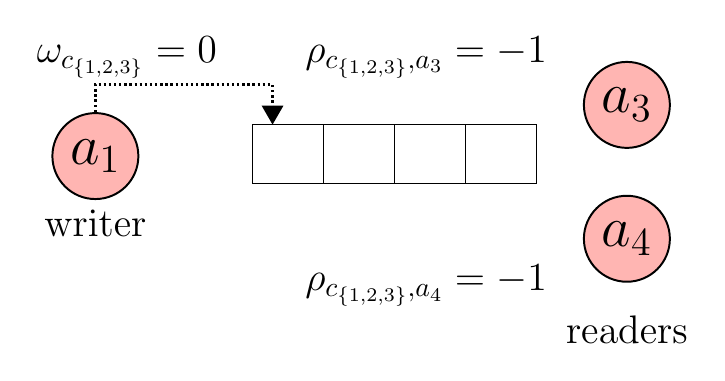
\begin{tikzpicture}
      \writingFIFOEmpty
    \end{tikzpicture}
    }
    \caption{\label{fig:MRBStateOne}Initial state of the \ac{MRB}}
  \end{subfigure}
  \begin{subfigure}[b]{0.48\columnwidth}
   \centering
    \resizebox{\columnwidth}{!}{
    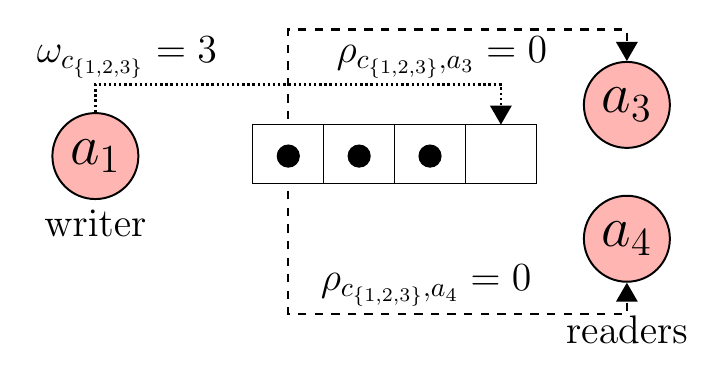
\begin{tikzpicture}
      \writingFIFO
    \end{tikzpicture}
    }
    \caption{\label{fig:MRBStateTwo}After firing $\langle \actor_1, \actor_1, \actor_1 \rangle$}
  \end{subfigure}
  \begin{subfigure}[b]{0.48\columnwidth}
   \centering
    \resizebox{\columnwidth}{!}{
    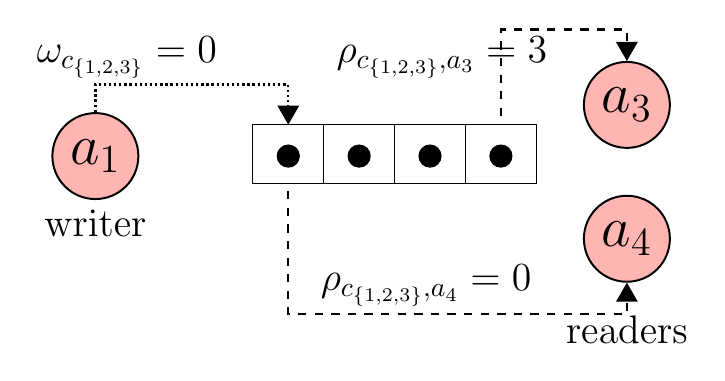
\begin{tikzpicture}
      \writingFIFOSecond
    \end{tikzpicture}
    }
    \caption{\label{fig:MRBStateThree}\ac{MRB} after $\langle \actor_3, \actor_3, \actor_3, \actor_1 \rangle$}
  \end{subfigure}
  \begin{subfigure}[b]{0.48\columnwidth}
   \centering
    \resizebox{\columnwidth}{!}{
    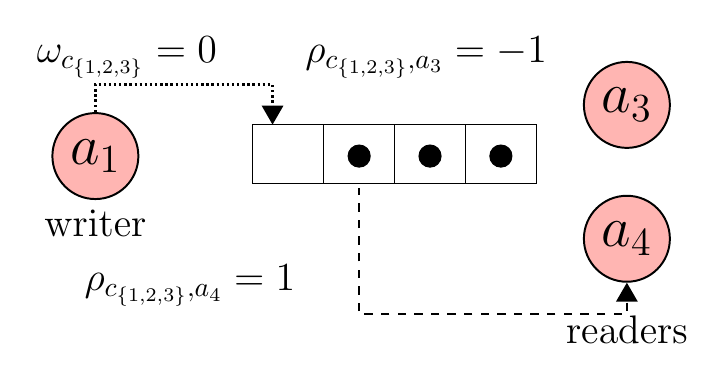
\begin{tikzpicture}
      \writingFIFOThird
    \end{tikzpicture}
    }
    \caption{\label{fig:MRBStateFour}\ac{MRB} after $\langle \actor_4, \actor_3 \rangle$}
  \end{subfigure}
  \caption{\label{fig:stateOfMRB}\ac{MRB} with one write index (pointer) indicating the location of the next token to be written.
    Moreover, each reading actor requires an index pointing to the position of the next token to read.\vspace{-3mm}}
\end{figure}
There, actors $\actor_1$, $\actor_3$, and $\actor_4$ are, respectively, associated with the write index $\Write_{\channel_{\{1,2,3\}}}$ and the read indices $\Read_{\channel_{\{1,2,3\}},\actor_3}$ and $\Read_{\channel_{\{1,2,3\}},\actor_4}$.
\par
Assuming the \ac{MRB} is initially empty, these read and write indices have the values shown in~\cref{fig:MRBStateOne}.
Thus, $\Tokens(\channel_{\{1,2,3\}}, \actor_3) = \Tokens(\channel_{\{1,2,3\}}, \actor_4) = 0$ and $\Free(\channel_{\{1,2,3\}}) = \Capacity(\channel_{\{1,2,3\}}) - \max \{ 0, 0 \} = 4$.
At this point (see~\cref{fig:MRBStateOne}), it is only possible to perform write operations.
Before firing $\actor_1$, we must check if there is at least one free place available for the produced token, i.e., $\Free(\channel_{\{1,2,3\}}) = 4 \geq 1$.
\par
Next, assume actor $\actor_1$ fires three times, resulting in the state shown in~\cref{fig:MRBStateTwo}.
There, the write index $\Write_{\channel_{\{1,2,3\}}}$ has advanced to $3$, pointing to the next free place in the \ac{MRB}'s buffer.
The read indices $\Read_{\channel_{\{1,2,3\}},\actor_3}$ and $\Read_{\channel_{\{1,2,3\}},\actor_4}$ have been updated during the first firing of actor $\actor_1$ from $-1$ to $0$, pointing to the first token contained in the \ac{MRB}.
At this point (see~\cref{fig:MRBStateTwo}), we can also perform read operations.
Before firing a reader, we need to verify if there exist sufficient tokens to be consumed by the reader.
For instance, we are able to fire actor $\actor_3$ because $\Tokens(\channel_{\{1,2,3\}}, \actor_3) = ((3-0-1)\ \mathrm{mod}\ 4) + 1 = 3 \geq 1$.
\par
After firing the sequence $\langle \actor_3, \actor_3, \actor_3, \actor_1 \rangle$, the resulting state is shown in~\cref{fig:MRBStateThree}.
There, the readers track different information about the state of the \ac{MRB}.
The reader $\actor_3$ points to $\Read_{\channel_{\{1,2,3\}},\actor_3}=3$ and observes $\Tokens(\channel_{\{1,2,3\}}, \actor_3)=((0-3-1)\ \mathrm{mod}\ 4)+1 = 1$ token, whereas reader $\actor_4$ points to $\Read_{\channel_{\{1,2,3\}},\actor_4}=0$ and observes $\Tokens(\channel_{\{1,2,3\}}, \actor_4)=((0-0-1)\ \mathrm{mod}\ 4)+1 = 4$ tokens.
From the perspective of the writer $\actor_1$, the \ac{MRB} is full.
At this point (see~\cref{fig:MRBStateThree}), let the firing sequence $\langle \actor_4, \actor_3 \rangle$ be observed.
\par
The resulting state of the \ac{MRB} is shown in \cref{fig:MRBStateFour}.
From the perspective of $\actor_3$, the \ac{MRB} is empty, i.e., $\Read_{\channel_{\{1,2,3\}},\actor_3}$ is $-1$.
The token placed at position $0$ has been consumed because $\actor_4$ has read it now, seeing $\Tokens(\channel_{\{1,2,3\}}, \actor_4)=((0-1-1)\ \mathrm{mod}\ 4)+1 = 3$ more tokens.
From the perspective of $\actor_1$, there is one free place as $\Free(\channel_{\{1,2,3\}}) = \Capacity(\channel_{\{1,2,3\}}) - \max \{ 0, 3 \} = 4 - 3 = 1$.

\subsection{Architecture Graph}\label{sec:architecture}
A heterogeneous many-core target architecture, e.g., as depicted in the right part of~\cref{fig:specification}, can be modeled formally by an abstract \emph{architecture graph}:
\begin{definition}[Architecture Graph]\label{def:architecture}
An architecture graph $\rgraph$ is a tuple $(\SetResources, \SetLinks)$ composed of a set of vertices $\SetResources$ modeling hardware resources and a set of edges $\SetLinks \subseteq \SetResources \times \SetResources$ denoting communication links between resources. 
\end{definition}
\par
Here, the set of vertices $\SetResources = \SetCores \cup \SetMemories \cup \SetInterconnects$ represents the resources of the architecture where each $\core \in \SetCores$ denotes a core, each $\memory \in \SetMemories$ a memory, and each $\interconnect \in \SetInterconnects$ an interconnect.
The set of cores $\SetCores$ is partitioned into sets $\SetCores_{\coretype_1}, \SetCores_{\coretype_2}, \ldots \SetCores_{\coretype_{|\SetCoreTypes|}}$.
Each set $\SetCores_\coretype$ describes the set of cores of identical core type $\coretype \in \SetCoreTypes$.
\par
The set of memory resources $\SetMemories = \SetMemoriesLocal \cup \SetTileLocalMemories \cup \{\GlobalMemory\}$ can be partitioned into \emph{core-local memories} ($\memory_{\core_i} \in \SetMemoriesLocal$), \emph{tile-local memories} ($\memory_{\tile_j} \in \SetTileLocalMemories$), and the \emph{global memory} ($\GlobalMemory$).
Each core $\core_i \in \SetCores$ has a core-local memory $\memory_{\core_i}$ reachable via a link $(\core_i,\memory_{\core_i}) \in \SetLinks$.
Each memory $\memory \in \SetMemories$ has a \emph{capacity} $\MemoryCapacity{\memory}$, which denotes the number of bytes that can be stored in the memory.
\par
The set of interconnects $\SetInterconnects$ is partitioned into the \ac{NoC} ($\NoC \in \SetInterconnects$) and a set of crossbars $\crossbar{} \in \SetCrossbars = \SetInterconnects \setminus \{\NoC\}$.
Each interconnect $\interconnect \in \SetInterconnects$ is annotated with its bandwidth $\Bandwidth{\interconnect}$, which is used to calculate data transfer delays.
The time required to transport $\eta$ bytes of data over a crossbar $\crossbar{}$ can be calculated as $\eta / \Bandwidth{\crossbar{}}$.
\par
Resources of a given architecture, excluding the \ac{NoC} and the global memory ($\GlobalMemory$), i.e., processors, local memories, tile-local memories, and crossbars, are organized as a set of tiles $\SetTiles$.
Each tile $\tile \in \SetTiles$ consists of a set of cores and their core-local memories, a tile-local memory, and a tile crossbar connecting the cores and memories of the tile.
As each resource belongs to exactly one tile, tiles are (i) \emph{disjoint}, i.e., $\forall \tile_i, \tile_j \in \SetTiles : \tile_i \cap \tile_j = \emptyset$ where $i \neq j$ and (ii) \emph{covering}, i.e., $\cup_{\tile \in \SetTiles} \tile = \SetResources \setminus \{ \GlobalMemory, \NoC \}$.
\par
Intra-tile communication is provided by links connecting each core and memory of the respective tile via the tile crossbar.
To exemplify, consider the tile $\tile_1$ presented in \cref{fig:specification}.
It is composed of six cores $\{\core_1,\ldots,\core_6\}$, six core-local memories $\{\memory_{\core_1},\ldots,\memory_{\core_6}\}$, the tile-local memory $\memory_{\tile_1}$, and the tile-crossbar $\crossbar{1}$.
Each core in tile $\tile_1$ has an exclusive communication link with its corresponding core-local memory, e.g., there exists a link $(\core_i,\memory_{\core_i})$ that connects core $\core_i$ with its memory $\memory_{\core_i}$.
Moreover, each memory of the tile can be reached via the tile-crossbar $\crossbar{1}$.
If core $\core_1$ sends data to $\core_4$, such data will traverse the tile-crossbar $\crossbar{1}$ via the links $(\core_1,\crossbar{1})$ and $(\crossbar{1},\memory_{\core_4})$ to be stored in the core-local memory $\memory_{\core_4}$ of core $\core_4$.
\par
For inter-tile communication, links are provided that connect each tile to the \ac{NoC} ($\NoC$), which in turn is connected to the global memory ($\GlobalMemory$).
\par
The set of resources involved in a data transfer between a core $\core$ and a memory $\memory$ will be denoted by a \emph{routing function} $\Routing: \SetCores \times \SetMemories \rightarrow \PowerSet{\SetResources}$%
\footnote{Here, the $\PowerSet{X}$ notation denotes the power set of the set $X$, i.e., the set of all subsets of $X$.}, as explained in the following.
\par
In the simplest case, a data transfer happens between a core $\core_i$ and its local memory $\memory_{\core_i}$.
Then, no interconnect resources are involved, i.e., $\Routing(\core_i, \memory_{\core_i}) = \{\core_i, \memory_{\core_i}\}$.
\par
Else, if the core $\core$ and the memory $\memory$ share the same tile ($\exists \tile_j \in \SetTiles: \core, \memory \in \tile_j$), an \emph{intra-tile} data transfer is performed.
In this case, the data transfer only traverses the tile crossbar $\crossbar{j}$, i.e., $\Routing(\core, \memory) = \{ \core, \crossbar{j}, \memory \}$.
\par
Otherwise, an \emph{inter-tile} transfer is needed as the core $\core$ and the memory $\memory$ are allocated in different tiles, i.e., $\core \in \tile_j$, $\memory \in \tile_k$, and $\tile_j \neq \tile_k$.
Then, the data needs to travel over the tile crossbar $\crossbar{j}$ of the tile containing the core $\core$, the \ac{NoC} interconnect $\NoC$, and the tile crossbar $\crossbar{k}$ of the tile containing the memory $\memory$, i.e., $\Routing(\core, \memory) = \{ \core, \crossbar{j}, \NoC, \crossbar{k}, \memory \}$.
\par
In all other cases, the global memory is used, and the involved interconnect resources are the tile crossbar $\crossbar{j}$ and the \ac{NoC}, i.e., $\Routing(\core, \GlobalMemory) = \{ \core, \crossbar{j}, \NoC, \GlobalMemory\}$.

\subsection{Specification graph}\label{sec:specification}

To perform explorations of allocations and mappings of actors to cores as well as channels to memories, a specification finally contains a set of \emph{mapping edges} $\SetMappings = \SetMappingsActors \cup \SetMappingsChannels$ that is partitioned into a set of potential mappings $\SetMappingsActors = \{ (\actor, \core) \in  \SetActors \times \SetCores \mid \exists \coretype \in \SetCoreTypes: \core \in \SetCores_\coretype \land \execTime(\actor, \coretype) \neq \bot \}$%
\footnote{Remember, $\execTime(\actor, \coretype) = \bot$ denotes that an actor $\actor$ cannot be mapped to a particular core type $\coretype$.}
of actors to cores and a set of potential mappings $\SetMappingsChannels = \SetChannels \times \SetMemories$ of channels to memories.
These mapping edges specify that every memory can store each channel and that each actor $\actor$ can be mapped to every core $\core \in \SetCores_\coretype$ of a type $\coretype$ that can execute the actor $\actor$.
With these definitions, a \emph{specification graph} can be defined as follows:
\begin{definition}[Specification Graph]
A specification graph $\sgraph$ is a tuple $(\SetSGVertices, \SetSGEdges)$ composed of a set of vertices $\SetSGVertices$ and a set of edges $\SetSGEdges$.
The set of vertices $\SetSGVertices = \SetActors \cup \SetChannels \cup \SetResources$ is formed from the union of vertices of the application graph $\pgraph$ and the architecture graph $\rgraph$.
Similarly, the set of edges $\SetSGEdges = \SetPGEdges \cup \SetLinks \cup \SetMappings$ is formed from the union of edges of both graphs and the set of \emph{mapping edges}.
\end{definition}
\Cref{fig:specification} illustrates an example of an application graph, an architecture graph, and an exemplified set of actor-to-core and channel-to-memory mappings.

\section{Definition of the Design Space}\label{sec:design-space}

This section introduces the \emph{design space} of selective \ac{MRB} replacements, formalizes the concept of actor and channel bindings, and illustrates the principles of actor and communication scheduling.

\subsection{Selective \ac{MRB} Replacement}\label{sec:mrb-substitution}

\begin{figure*}[t!]
  \centering
  \scalebox{1.0}{\input{figs/schedMRBQP3-fig.tex}}
  \caption{\label{fig:schedMRBQP3}Example of a schedule with period $\Period=8$ time steps (right) for the transformed application graph $\mrbgraph$ from~\cref{fig:mergingChannel} where actors $\actor_1$ and $\actor_5$ are bound to core $\core_3$, actor $\actor_3$ and channel $\channel_4$ are bound to core $\core_1$ and its core-local memory $\memory_{\core_1}$, as well as actor $\actor_4$ and channel $\channel_5$ are bound to core $\core_2$ and its core-local memory $\memory_{\core_2}$.
    For better visualization, we use $\GenMRB$ to refer to the \ac{MRB} $\channel_{\{1,2,3\}}$, which is bound to the core-local memory $\memory_{\core_3}$ of core $\core_3$ (left).
    The light red boxes in the Gantt chart shown to the right denote actor executions, while the light green boxes denote read operations, e.g., the light green box containing $(\channel_4, \actor_5)$ denotes a read of a token contained in channel $\channel_4$ by the actor $\actor_5$.
    The data dependencies of the application graph $\mrbgraph$ are depicted by the solid and dotted dashed directed edges in the Gantt chart.
    For example, the solid directed edge from actor $\actor_1$ over the read communication $(\GenMRB,\actor_4)$ to actor $\actor_4$ represents the data dependency between actors $\actor_1$ and $\actor_4$ communicated via the \ac{MRB} $\GenMRB$.
    The Gantt chart does not depict the corresponding write $(\actor_1,\GenMRB)$ as the \ac{MRB} $\GenMRB$ is bound to the core-local memory $\memory_{\core_3}$ of the core $\core_3$, where actor $\actor_1$ is bound to.
    Thus, the write communication is assumed to be part of the execution of actor $\actor_1$ itself.}
\end{figure*}

As discussed in~\cref{sec:multi-cast-actors}, each multi-cast actor represents an opportunity for memory footprint reduction by replacing it and its adjacent channels with an \ac{MRB}, as shown in~\cref{fig:fifoRealizations}.
However, replacing a multi-cast actor with an \ac{MRB} may also lead to an increase in the \emph{execution period}~\cite{lft_2023-MRBs}, which is defined as the time interval between two successive iterations of execution of a given application graph.
Hence, which multi-cast actors are replaced by \acp{MRB} needs to be explored to trade between period and memory footprint, both to be minimized.
For this purpose, we define a multi-cast actor \emph{replacement} function $\useMRB: \SetActorsMulticast \rightarrow \{ 0, 1 \}$ to determine for each multi-cast actor $\actorMulticast \in \SetActorsMulticast$ if it should be replaced by an \ac{MRB} ($\useMRB(\actorMulticast) = 1$) or kept ($\useMRB(\actorMulticast) = 0$).
\par
Formally, the replacement of selected multi-cast actors with \acp{MRB} for a given application graph $\pgraph$ (e.g., as illustrated in~\cref{fig:TokenBased}) can be realized by a graph transformation as detailed in~\cref{alg:merging}, leading to a transformed application graph $\mrbgraph$ (e.g., as shown in~\cref{fig:mergingChannel}), where the selected multi-cast actors and the channels connected to them have been replaced by their corresponding \acp{MRB}.
\par
\revised{The complexity of the selective \ac{MRB} replacement presented in~\cref{alg:merging} depends on how the graph topology is stored.
Assuming an implementation storing for each vertex its adjacency in a hash set, enabling edge addition and removal in an average time complexity of $O(1)$, the complexity of~\cref{alg:merging} is $O(|\SetActors| + |\SetChannels|)$, where $|\SetActors|$ is the upper bound of the number of replaced multi-cast actors and $|\SetChannels|$ is an upper bound of the number of removed channels and edges (respectively $2\cdot|\SetChannels|$).}
%\revised{Finally, the complexity of the selective \ac{MRB} replacement presented in \cref{alg:merging} depends on how the graph topology is stored.
%For our analysis, we assume that for each vertex, the set of adjacent vertices is given by an adjacency list of this vertex.
%Hence, the set of edges $\SetPGEdges$ does not need to be searched for this information, but the adjacency list of a vertex can be consulted in $O(1)$, e.g., to obtain $\SetChannels_\textrm{del}$ in \cref{alg:merging:search} and the edges $(\actor,\channel)$ and $(\channel,\actor)$ for a given channel $\channel \in \SetChannels_\textrm{del}$ in \cref{alg:merging:loop1,alg:merging:loop3}.
%Remember that for each channel, there exist exactly two adjacent actors.
%Moreover, we assume double-linked lists so that insertion and deletion can be performed in $O(1)$ (see \cref{alg:merging:loop2,alg:merging:loop4,alg:merging:loop5,alg:merging:loop6}).
%With these assumptions, the complexity of \cref{alg:merging} is $O(|\SetActorsMulticast| + |\SetChannels|)$.
%The $|\SetActorsMulticast|$ part comes from the outer loop in \cref{alg:merging:for}.
%The $|\SetChannels|$ comes from the channel replacements.
%Each replacement (see \cref{alg:merging:loop1,alg:merging:loop2,alg:merging:loop3,alg:merging:loop4,alg:merging:loop6}) can be performed in $O(1)$.
%Thus, at most $|\SetChannels|$ replacements can be performed.}
%\revised{Finally, the complexity of the selective \ac{MRB} replacement presented in \cref{alg:merging} is $O(|\SetActorsMulticast| + |\SetChannels|)$.
%The complexity of the presented replacement is dominated by the for loop in \cref{alg:merging:for}, which has to check all the multicast actors $\SetActorsMulticast$ and by the search of channels $\SetChannels_\textrm{del}$ connected at the input and outputs of the each multicast actor $\actorMulticast$  to replace (see \cref{alg:merging:search}).}
\begin{algorithm}[h!]
  \footnotesize
  \caption{Selective \acs{MRB} Replacement}\label{alg:merging}
  \SetKwProg{Fn}{Function}{}{}
  \SetKwFunction{FSubstituteMRBs}{substituteMRBs}
  \SetKwInOut{Input}{Input}
  \SetKwInOut{Output}{Output}
  \Fn{\FSubstituteMRBs{$\pgraph, \useMRB$}}{
    \Input{Application graph $\pgraph$ and function $\useMRB$}
    \Output{Transformed application graph $\mrbgraph$}
    \BlankLine
    $\mrbgraph \leftarrow \pgraph$\tcp*[f]{\footnotesize Let $\mrbgraph$ be a copy of $\pgraph$}\\
    \tcc{\footnotesize Only replace $\actorMulticast$ when $\useMRB(\actorMulticast) = 1$}
    \ForEach{\normalfont $\actorMulticast \in \SetActorsMulticast$ \textit{where} $\useMRB(\actorMulticast) = 1$}{ \label{alg:merging:for}
      \tcc{\footnotesize Let $\SetChannels_\textrm{del}$ be the set of all channels that are adjacent to $\actorMulticast$}
      $\SetChannels_\textrm{del} \leftarrow \{ \channel \in \mrbgraph.\SetChannels \mid (\channel, \actorMulticast) \in \mrbgraph.\SetPGEdges \vee (\actorMulticast, \channel) \in \mrbgraph.\SetPGEdges \}$\label{alg:merging:search} \\
      \tcc{\footnotesize New \ac{MRB} channel $\GenMRB$}
      $\GenMRB \leftarrow \text{createMRB}(\SetChannels_\textrm{del})$\\
      \tcc{\footnotesize Add an input edge to $\GenMRB$, replacing the ones for $\actorMulticast$}
      \ForEach{\normalfont $(\actor, \channel) \in \mrbgraph.\SetPGEdges$ \textit{where} $\channel \in \SetChannels_\textrm{del} \wedge \actor \neq \actorMulticast$}{\label{alg:merging:loop1}
        $\mrbgraph.\SetPGEdges \leftarrow \{(\actor, \GenMRB)\} \cup \mrbgraph.\SetPGEdges \setminus \{(\actor, \channel), (\channel, \actorMulticast)\}$\label{alg:merging:loop2}
%       $\Delay(\GenMRB) \leftarrow \Delay(\channel)$ \tcp*[f]{\footnotesize Set initial tokens for \ac{MRB}}\\
%       $\Size(\GenMRB) \leftarrow \Size(\channel)$   \tcp*[f]{\footnotesize Set token size of \ac{MRB}}\\
      }
      \tcc{\footnotesize Add output edges from $\GenMRB$, replacing the ones for $\actorMulticast$} 
      \ForEach{\normalfont $(\channel, \actor) \in \mrbgraph.\SetPGEdges$ \textit{where} $\channel \in \SetChannels_\textrm{del} \wedge \actor \neq \actorMulticast$}{\label{alg:merging:loop3}
        $\mrbgraph.\SetPGEdges \leftarrow \{(\GenMRB, \actor)\} \cup \mrbgraph.\SetPGEdges \setminus \{(\actorMulticast, \channel), (\channel, \actor)\}$ \label{alg:merging:loop4}
%       $\Capacity(\GenMRB) \leftarrow \Capacity(\channel') + \Capacity(\channel'')$ \tcp*[f]{\footnotesize Set capacity of \ac{MRB}} \label{alg2:adjustCapacity}\\
      }
     $\mrbgraph.\SetActors \leftarrow \mrbgraph.\SetActors \setminus \{\actorMulticast\}$\tcp*[f]{\footnotesize Remove $\actorMulticast$} \label{alg:merging:loop5} \\
     $\mrbgraph.\SetChannels \leftarrow \{\GenMRB\} \cup \mrbgraph.\SetChannels \setminus \SetChannels_\textrm{del}$\tcp*[f]{\footnotesize Replace $\SetChannels_\textrm{del}$ by $\GenMRB$} \label{alg:merging:loop6} \\
    }
    \Return $\mrbgraph$
  }
\end{algorithm}
\begin{algorithm}[t!]
  \footnotesize
  \caption{Determine Channel Bindings $\SetBindingsChannels$}\label{alg:determine-channel-bindings}
  \SetKwProg{Fn}{Function}{}{}
  \SetKwFunction{FChannelBindings}{determineChannelBindings}
  \SetKwInOut{Input}{Input}
  \SetKwInOut{Output}{Output}
% \SetKwRepeat{Do}{do}{while}
% \SetKwFunction{FHelp}{fireable}
% \SetKwFunction{FAvailable}{AvailableCoresPerTile}
% \SetKwFor{Case}{case}{}{end case}%
  \SetKw{Break}{break}
  \Fn{\FChannelBindings{$\ChannelDecisions, \Capacity, \SetBindingsActors$}}{
    \Input{Channel decision function $\ChannelDecisions$, channel capacity function $\Capacity$, and the set of actor bindings $\SetBindingsActors$}
    \Output{The set of channel bindings $\SetBindingsChannels$}
    \BlankLine
    $\memoryUsage{\memory} \leftarrow 0\enspace\forall \memory \in \SetMemories$\tcp*[f]{\footnotesize Start memory usage $\memoryUsage{\memory}$ from 0}\\
    $\SetBindingsChannels \leftarrow \emptyset$\tcp*[f]{\footnotesize Start with empty bindings $\SetBindingsChannels$}\\
    \tcp{\footnotesize Derive binding for each channel $\channel \in \SetChannels$}
    \ForEach{$\channel \in \SetChannels$}{
      \tcc{\footnotesize Derive $\actor_{prod}$, $\core_{prod}$, $\tile_{prod}$, $\actor_{cons}$, $\core_{cons}$, and $\tile_{cons}$ for channel $\channel$}
      $\actor_{prod} \in \SetActors$ such that $(\actor_{prod},\channel) \in \SetPGEdges$\tcp*[f]{\footnotesize Derive $\actor_{prod}$}\\
      $\core_{prod} \in \SetCores$ such that $(\actor_{prod},\core_{prod}) \in \SetBindingsActors$\tcp*[f]{\footnotesize Derive $\core_{prod}$}\\
      $\tile_{prod} \in \SetTiles$ such that $\core_{prod} \in \tile_{prod}$\tcp*[f]{\footnotesize Derive $\tile_{prod}$}\\
      $\actor_{cons} \in \SetActors$ such that $(\channel, \actor_{cons}) \in \SetPGEdges$\tcp*[f]{\footnotesize Derive $\actor_{cons}$}\\
      $\core_{cons} \in \SetCores$ such that $(\actor_{cons},\core_{cons}) \in \SetBindingsActors$\tcp*[f]{\footnotesize Derive $\core_{cons}$}\\
      $\tile_{cons} \in \SetTiles$ such that $\core_{cons} \in \tile_{cons}$\tcp*[f]{\footnotesize Derive $\tile_{cons}$}\\
      \Switch{$\ChannelDecisions(\channel)$}{
        \Case{\texttt{PROD}}{
          \If{$\memoryUsage{\memory_{\core_{prod}}} + \Capacity(\channel) \cdot \Size(\channel) \leq \MemoryCapacity{\memory_{\core_{prod}}}$}{
            \tcp{\footnotesize Bind $\channel$ to $\memory_{\core_{prod}}$}
            $\SetBindingsChannels \leftarrow \SetBindingsChannels \cup \{ (\channel, \memory_{\core_{prod}}) \}$\\
            $\memoryUsage{\memory_{\core_{prod}}} \leftarrow \memoryUsage{\memory_{\core_{prod}}} + \Capacity(\channel) \cdot \Size(\channel)$\\
            \Break
          }
          \tcp{\footnotesize $\memory_{\core_{prod}}$ too small, try $\memory_{\tile_{prod}}$ next}
        }
        \Case{\texttt{TILE-PROD}}{
          \If{$\memoryUsage{\memory_{\tile_{prod}}} + \Capacity(\channel) \cdot \Size(\channel) \leq \MemoryCapacity{\memory_{\tile_{prod}}}$}{
            \tcp{\footnotesize Bind $\channel$ to $\memory_{\tile_{prod}}$}
            $\SetBindingsChannels \leftarrow \SetBindingsChannels \cup \{ (\channel, \memory_{\tile_{prod}}) \}$\\
            $\memoryUsage{\memory_{\tile_{prod}}} \leftarrow \memoryUsage{\memory_{\tile_{prod}}} + \Capacity(\channel) \cdot \Size(\channel)$\\
            \Break
          }
          \tcp{\footnotesize $\memory_{\tile_{prod}}$ too small, bind to $\GlobalMemory$}
          $\SetBindingsChannels \leftarrow \SetBindingsChannels \cup \{ (\channel, \GlobalMemory) \}$\\
          \Break
        }
        \Case{\texttt{CONS}}{
          \If{$\memoryUsage{\memory_{\core_{cons}}} + \Capacity(\channel) \cdot \Size(\channel) \leq \MemoryCapacity{\memory_{\core_{cons}}}$}{
            \tcp{\footnotesize Bind $\channel$ to $\memory_{\core_{cons}}$}
            $\SetBindingsChannels \leftarrow \SetBindingsChannels \cup \{ (\channel, \memory_{\core_{cons}}) \}$\\
            $\memoryUsage{\memory_{\core_{cons}}} \leftarrow \memoryUsage{\memory_{\core_{cons}}} + \Capacity(\channel) \cdot \Size(\channel)$\\
            \Break
          }
          \tcp{\footnotesize $\memory_{\core_{cons}}$ too small, try $\memory_{\tile_{cons}}$ next}
        }
        \Case{\texttt{TILE-CONS}}{
          \If{$\memoryUsage{\memory_{\tile_{cons}}} + \Capacity(\channel) \cdot \Size(\channel) \leq \MemoryCapacity{\memory_{\tile_{cons}}}$}{
            \tcp{\footnotesize Bind $\channel$ to $\memory_{\tile_{cons}}$}
            $\SetBindingsChannels \leftarrow \SetBindingsChannels \cup \{ (\channel, \memory_{\tile_{cons}}) \}$\\
            $\memoryUsage{\memory_{\tile_{cons}}} \leftarrow \memoryUsage{\memory_{\tile_{cons}}} + \Capacity(\channel) \cdot \Size(\channel)$\\
            \Break
          }
          \tcp{\footnotesize $\memory_{\tile_{cons}}$ too small, bind to $\GlobalMemory$}
        }
        \Case{\texttt{GLOBAL}}{
          \tcp{\footnotesize Bind $\channel$ to $\GlobalMemory$}
          $\SetBindingsChannels \leftarrow \SetBindingsChannels \cup \{ (\channel, \GlobalMemory) \}$\\
        }
      }
    }
    \Return $\SetBindingsChannels$
  }
\end{algorithm}

\subsection{Actor and Channel Bindings} \label{sec:ActorChannelBindings}

Next, determining an implementation of a transformed application graph $\mrbgraph$ on an architecture requires a binding (i) of each actor to a processor, which is described by a set $\SetBindingsActors \subseteq \SetMappingsActors$ called \emph{actor bindings}, and (ii) of each channel to a memory, which is described by a set $\SetBindingsChannels \subseteq \SetMappingsChannels$ called \emph{channel bindings}.
Moreover, each actor and channel must be bound to exactly one core (see~\cref{eq:actorBinding}), respectively, memory (see~\cref{eq:channelBinding}).
Finally, the channels bound to a memory $\memory \in \SetMemories$ must not exceed its capacity (see~\cref{eq:memoryConstraint}).
A set of \emph{feasible bindings} $\SetBindings = \SetBindingsActors \cup \SetBindingsChannels$ must satisfy \crefrange{eq:actorBinding}{eq:memoryConstraint}.
\par
\begin{align}
  \forall \actor \in \SetActors     &:& | \SetBindingsActors \cap (\{\actor\} \times \SetCores)|& = 1&  \label{eq:actorBinding}\\
  \forall \channel \in \SetChannels &:& | \SetBindingsChannels \cap (\{\channel\} \times \SetMemories)|& = 1& \label{eq:channelBinding}\\
  \forall \memory \in \SetMemories  &:& \sum_{(\channel,\memory) \in \SetBindingsChannels} \Capacity(\channel) \cdot \Size(\channel) &\leq \MemoryCapacity{\memory}& \label{eq:memoryConstraint}
\end{align}
\par
The number of cores $\allocation(\coretype)$ allocated of a given type $\coretype$ can then be implicitly derived from the actor binding $\SetBindingsActors$ as \emph{allocation} $\allocation$.
\begin{equation}
  \allocation(\coretype) = |\{ \core \in \SetCores_\coretype \mid \exists (\actor, \core) \in \SetBindingsActors \}|
\end{equation}
\par
For example, the actor and channel bindings shown in \cref{fig:schedMRBQP3} are given by $\SetBindingsActors = \{(\actor_3,\core_1), (\actor_4,\core_2), (\actor_1,\core_3), (\actor_5,\core_3)\}$ and $\SetBindingsChannels = \{(\channel_4,\memory_{\core_1}), (\channel_5,\memory_{\core_2}), (\GenMRB,\memory_{\core_3})\}$, respectively.
From these, the core allocations $\allocation(\coretype_1) = 2$, $\allocation(\coretype_2) = 1$, and $\allocation(\coretype_3) = 0$ can be derived.
Moreover, the notation $\SetBindingsActors(\actor)$ and $\SetBindingsChannels(\channel)$ denote the core and memory the actor $\actor$, respectively, channel $\channel$ are bound to, e.g., $\SetBindingsActors(\actor_3) = \core_1$ and $\SetBindingsChannels(\channel_4) = \memory_{\core_1}$.
\par
While, in principle, each channel $\channel \in \SetChannels$ can be bound to any memory $\memory \in \SetMemories$, it makes sense to constrain the design space to be explored such that a channel will not be bound to a core-local memory of a core that does not at all access the channel data.
Similarly, tile-local memories of tiles containing no core accessing the channel data can also be excluded.
As a result, only five binding alternatives exist for each channel:
(\texttt{PROD}) the core-local memory $\memory_{\core_{prod}}$ of the core $\core_{prod}$ producing the data,
(\texttt{TILE-PROD}) the tile-local memory $\memory_{\tile_{prod}}$ of the tile $\tile_{prod}$ containing the core producing the data,
(\texttt{CONS}) the core-local memory  $\memory_{\core_{cons}}$ of the core $\core_{cons}$ consuming the data,
(\texttt{TILE-CONS}) the tile-local memory $\memory_{\tile_{cons}}$ of the tile $\tile_{cons}$ containing the core consuming the data, or
(\texttt{GLOBAL}) the global memory $\GlobalMemory$.
\par
In the following, these five options are represented by a \emph{channel decision} function $\ChannelDecisions: \SetChannels \rightarrow \{$\texttt{GLOBAL}, \texttt{TILE-PROD}, \texttt{TILE-CONS}, \texttt{PROD}, \texttt{CONS}$\}$, which shall be explored rather than exploring channel bindings directly.
Concrete channel bindings $\SetBindingsChannels$ can then be determined via~\cref{alg:determine-channel-bindings} from the channel decisions, channel capacities, and actor bindings in such a way that~\cref{eq:channelBinding,eq:memoryConstraint} are satisfied.
\Cref{alg:determine-channel-bindings} determines for each channel $\channel \in \SetChannels$ a concrete binding according to the channel decision $\ChannelDecisions(\channel)$ in case memory capacities $\MemoryCapacity{\memory}$ are not exceeded.
Otherwise, a fallback solution is determined according to the case statements.
It can be proven that a feasible binding is always found for each channel $\channel \in \SetChannels$ by binding $\channel$ to the global memory $\GlobalMemory$ that is assumed to be large enough to store all the buffer data related to the channels of a given application.
\revised{Since the channel decision requires checking each channel $\channel \in \SetChannels$, the complexity of~\cref{alg:determine-channel-bindings} is $O(|\SetChannels|)$, thus linear in the number of channels $|\SetChannels|$ of a given application.}
\par
\Cref{alg:determine-channel-bindings} derives the channel bindings. 
For the running example in~\cref{fig:schedMRBQP3}, we obtain $\SetBindingsChannels = \{(\channel_4,\memory_{\core_1}),$ $(\channel_5,\memory_{\core_2}),$ $(\GenMRB,\memory_{\core_3})\}$ from the channel decisions $\ChannelDecisions(\channel_4) =$ $\ChannelDecisions(\channel_5) =$ $\ChannelDecisions(\GenMRB) = \texttt{PROD}$ and the actor bindings $\SetBindingsActors = \{(\actor_3,\core_1),$ $(\actor_4,\core_2),$ $(\actor_1,\core_3),$ $(\actor_5,\core_3)\}$.
\Cref{alg:determine-channel-bindings} thereby prefers to bind channels to core-local memories.
If the core-local memory ($\memory_{\core_3}$ in the running example) did not have a sufficient capacity to accommodate the \ac{MRB} channel $\GenMRB$, \cref{alg:determine-channel-bindings} would bind $\GenMRB$ to the tile-local memory $\memory_{\tile_1}$, and if even $\memory_{\tile_1}$ would also have an insufficient capacity, the channel $\GenMRB$ would finally be bound to the global memory $\GlobalMemory$.

\subsection{Periodic Scheduling of Actors and Communication}
In the following, we  consider the optimization and generation of static periodic schedules with an assumed uninterrupted execution of actors and communications.
We also assume that each actor executes on the same core for each iteration of the dataflow graph.
As it is assumed that the underlying \ac{DFG} of a given application graph $\mrbgraph$ is a marked graph~\cite{chep_1971-marked-graphs}, for each actor $\actor \in \mrbgraph.\SetActors$, read $(\channel,\actor) \in \mrbgraph.\SetPGEdges$, as well as write $(\actor,\channel) \in\mrbgraph.\SetPGEdges$ operation, we need to determine exactly one \emph{start time} $\startTime_\actor$, $\startTime_{(\channel,\actor)}$, and $\startTime_{(\actor,\channel)}$, respectively, which repeats with the period $\Period$.
Thus, the actors and edges of the application graph $\mrbgraph$ together define the set of tasks to be scheduled, i.e., $\task \in \SetTasks = \mrbgraph.\SetActors \cup \mrbgraph.\SetPGEdges$.

For example, consider the schedule with a period of $\Period = 7$ depicted in~\cref{fig:schedOptPeriod} with actor start times as follows: $\startTime_{\actor_1} = 0$, $\startTime_{\actor_2} = 1$, $\startTime_{\actor_3} = 3$, $\startTime_{\actor_4} = 4$, and $\startTime_{\actor_5} = 13$.
Note that the start time of actor $\actor_5$ is greater than the period.
Therefore, the firing of actor $\actor_5$ depicted in the schedule at time step $6$ belongs to the previous iteration.
Naturally, start times also need to be determined for the read and write operations, e.g., $\startTime_{(\actor_2,\channel_2)} = 2$, $\startTime_{(\actor_2,\channel_3)} = 3$, $\startTime_{(\channel_4,\actor_5)} = 11$, and $\startTime_{(\channel_5,\actor_5)} = 12$ for the write and read operations shown in the schedule.
The read and write operations with assumed zero communication time (i.e., read and write operations not involving any interconnect resource), which are not depicted in the schedule, have the following start times: $\startTime_{(\actor_1,\channel_1)} = \startTime_{(\channel_1,\actor_2)} = 1$ (i.e., after actor $\actor_1$ has finished and before actor $\actor_2$ starts), $\startTime_{(\channel_2,\actor_3)} = 3$ (i.e., before actor $\actor_3$ starts), $\startTime_{(\channel_3,\actor_4)} = 4$ (i.e., before actor $\actor_4$ starts), $\startTime_{(\actor_3,\channel_4)} = 10$ (i.e., after actor $\actor_3$ finishes), and $\startTime_{(\actor_4,\channel_5)} = 11$ (i.e., after actor $\actor_4$ finishes).

Furthermore, for each actor $\actor$, its execution time is denoted by $\execTime_\actor$, derivable from the actor bindings $\SetBindingsActors$ as follows:
\begin{align}
  \execTime_\actor     = & \execTime(\actor, \coretype) \textrm{ where } \coretype \in \SetCoreTypes \textrm{ such that } \SetBindingsActors(\actor) \in \SetCores_\coretype
\end{align}
\par
For example, the actor execution times $\execTime_{\actor_1} = \execTime_{\actor_2} = \execTime_{\actor_5} = 1$ and $\execTime_{\actor_3} = \execTime_{\actor_4} = 7$ correspond to those depicted in the schedule shown in~\cref{fig:schedOptPeriod}.

The time required for one token to be read from, respectively, written to channel $\channel$ by actor $\actor$ is denoted by $\execTime_{(\channel, \actor)}$ and $\execTime_{(\actor, \channel)}$.
In the following, these times are derived from the token size $\Size(\channel)$ and the interconnect bandwidth $\Bandwidth{\interconnect}$ of the interconnect $\interconnect$ with the minimal bandwidth that is traversed by the communication:
\begin{equation}
  \execTime_{(\channel,\actor)} = \execTime_{(\actor,\channel)} = \Size(\channel) / \min_{\interconnect \in \Routing(\SetBindingsActors(\actor), \SetBindingsChannels(\channel)) \cap \SetInterconnects} \Bandwidth{\interconnect}
\end{equation}
\begin{figure*}[t!]
  \centering
  \scalebox{1.0}{\input{figs/schedOptPeriod-fig.tex}}
  \caption{\label{fig:schedOptPeriod}Schedule with a period of $\Period = 7$ (shown to the right) for the application graph $\pgraph$ from~\cref{fig:TokenBased}.
    Actor $\actor_3$ is bound to core $\core_1$, actor $\actor_4$ is bound to core $\core_2$, and actors $\actor_1$, $\actor_2$, and $\actor_5$ are bound to core $\core_3$.
    Channels $\channel_2$ and $\channel_4$ are bound to the core-local memory $\memory_{\core_1}$, channels $\channel_3$ and $\channel_5$ are bound to core-local memory $\memory_{\core_2}$, and channel $\channel_1$ is bound to core-local memory $\memory_{\core_3}$ (shown to the left).
    The light red boxes and the light violet box (for the multi-cast actor $\actor_2$) in the Gantt chart shown to the right denote actor executions, the green boxes represent write operations, and the light green boxes indicate read operations.
    To exemplify, the green box containing $(\actor_2, \channel_2)$ represents a write of a token to channel $\channel_2$ by the actor $\actor_2$, and the light green box containing $(\channel_4, \actor_5)$ indicates a read of a token contained in channel $\channel_4$ by the actor $\actor_5$.
    Similarly to~\cref{fig:schedMRBQP3}, the data dependencies of the application graph $\pgraph$ are depicted by the solid and dotted dashed directed edges in the Gantt chart.
    The read and write from and to channel $\channel_1$ are not shown in the Gantt chart as both the write $(\actor_1,\channel_1)$ of actor $\actor_1$ to channel $\channel_1$ and the read $(\channel_1,\actor_2)$ of actor $\actor_2$ from channel $\channel_1$ access the core-local memory $\memory_{\core_3}$ of the core $\core_3$ that executes both actors $\actor_1$ and $\actor_2$.
    Thus, the corresponding write and read communication times are zero, i.e., $\execTime_{(\actor_1,\channel_1)} = \execTime_{(\channel_1,\actor_2)} = 0$, as the communication is assumed to be part of the execution of the actors themselves.
    The same situation holds for the read from channel $\channel_2$ and write to channel $\channel_4$ by actor $\actor_3$ as well as the read from channel $\channel_3$ and write to channel $\channel_5$ by actor $\actor_4$, i.e., $\execTime_{(\channel_2,\actor_3)} = \execTime_{(\actor_3,\channel_4)} = \execTime_{(\channel_3,\actor_4)} = \execTime_{(\actor_4,\channel_5)} = 0$.}
\end{figure*}
As a consequence, read and write operations that do not traverse at least one interconnect resource have zero communication time, e.g., $\execTime_{(\actor_1,\channel_1)} = \execTime_{(\channel_1,\actor_2)} = \execTime_{(\channel_2,\actor_3)} = \execTime_{(\actor_3,\channel_4)} = \execTime_{(\channel_3,\actor_4)} = \execTime_{(\actor_4,\channel_5)} = 0$ for the actor and channel bindings given in~\cref{fig:schedOptPeriod}.
Such communication operations directly access a core-local memory $\memory_{\core_i}$ from the corresponding core $\core_i$.
In this case, the communication is assumed to be part of the execution of the actor performing the read or write operation.
In other cases, the traversed interconnect resource $\interconnect$ with an assumed minimal bandwidth $\Bandwidth{\interconnect}$ leads to a non-zero communication time.
In the example above, $\execTime_{(\actor_2,\channel_2)} = \execTime_{(\actor_2,\channel_3)} = \execTime_{(\channel_4,\actor_5)} =  \execTime_{(\channel_5,\actor_5)} = 1$, as visualized in the schedule in~\cref{fig:schedOptPeriod}.

Finally, let $\SetActors_\resource$ and $\SetTasks_\resource$ denote the set of actors, respectively, tasks mapped to a resource $\resource$.
Formally, $\SetActors_\resource$ can be derived from the set of actor bindings $\SetBindingsActors$ as follows:
\begin{align}
  \SetActors_\resource = &\{ \actor \in \mrbgraph.\SetActors \mid \resource = \SetBindingsActors(\actor) \}
\end{align}
For a fully formal definition of $\SetTasks_\resource$, we extend the domain of the routing function $\Routing$ to also contain all edges $\edge \in \mrbgraph.\SetPGEdges$ of the application graph $\mrbgraph$.
Given the bindings $\SetBindingsActors$ and $\SetBindingsChannels$, let the set of resources involved by a write operation $\edge = (\actor, \channel)$ or read operation $\edge = (\channel, \actor)$  be denoted by $\Routing(\actor, \channel) = \Routing(\SetBindingsActors(\actor), \SetBindingsChannels(\channel))$, respectively, $\Routing(\channel, \actor) = \Routing(\SetBindingsActors(\actor), \SetBindingsChannels(\channel))$.
With this extension, $\SetTasks_\resource$ is given by:
\begin{align}
  \SetTasks_\resource  = &\{ \edge \in \mrbgraph.\SetPGEdges \mid \resource \in \Routing(\edge) \} \cup \SetActors_\resource
\end{align}
\par
%\vspace{-1mm}
For example, the set of all actors bound to core $\core_3$, as shown in~\cref{fig:schedOptPeriod}, is given by $\SetActors_{\core_3} = \{ \actor_1, \actor_2, \actor_5 \}$.
Including read and write operations executed by core $\core_3$ results in the set $\SetTasks_{\core_3} = \SetActors_{\core_3} \cup \{ (\actor_1,\channel_1), (\channel_1,\actor_2), (\actor_2,\channel_2), (\actor_2,\channel_3), (\channel_4,\actor_5), (\channel_5,\actor_5) \}$.
Note that the write $(\actor_1,\channel_1)$ and the read $(\channel_1,\actor_2)$ are not shown in the schedule depicted in~\cref{fig:schedOptPeriod}, as these are assumed to have zero communication times.
Moreover, read and write operations are, in general, bound to multiple resources, as they are bound to the core where the data is produced or consumed as well as all traversed interconnect resources, e.g., the read and write operations $(\actor_2,\channel_2)$, $(\actor_2,\channel_3)$, $(\channel_4,\actor_5)$, and $(\channel_5,\actor_5)$ are not only executed by core $\core_3$ but are also traversing the interconnect $\crossbar{1}$, i.e., $\SetTasks_\crossbar{1} = \{ (\actor_2,\channel_2), (\actor_2,\channel_3), (\channel_4,\actor_5), (\channel_5,\actor_5) \}$.

\subsection{Trade-offs between the Minimization of Memory Footprint and the Achievable Period}\label{sec:MFvsPeriod}

Replacing a multi-cast actor and its adjacent channels with an \ac{MRB} has as its primary purpose the reduction of the memory footprint (see~\cref{fig:fifoRealizations}).
Moreover, this transformation removes both the need to execute the multi-cast actor and its communication.
Nonetheless, there are cases where an \ac{MRB} replacement is detrimental to (i.e., it increases) the execution period $\Period$.
To illustrate this, \cref{fig:schedMRBQP3,fig:schedOptPeriod} present two periodic schedules obtained from the specification shown in~\cref{fig:specification}.
One can see that the schedule shown in~\cref{fig:schedMRBQP3} utilizing an \ac{MRB} has a longer period, i.e., $\Period = 8$, than the schedule with period $\Period = 7$ depicted in~\cref{fig:schedOptPeriod}, where the multi-cast actor $\actor_2$ has been retained.
The timings in \cref{fig:schedMRBQP3,fig:schedOptPeriod} are chosen for illustrative purposes to demonstrate the impact of \acp{MRB} and the existing trade-off in the specification.
In both schedules, the same actor-to-core binding is assumed for actors $\actor_1, \actor_3, \actor_4$, and $\actor_5$, i.e., actors $\actor_1$ and $\actor_5$ are bound to core $\core_3$, actor $\actor_3$ is bound to core $\core_1$, and actor $\actor_4$ is bound to core $\core_2$.
Moreover, channels $\channel_4$ and $\channel_5$ are bound to the core-local memories $\memory_{\core_1}$ and $\memory_{\core_2}$, respectively.

As mentioned previously, the illustrated schedules are distinguished whether they employ an \ac{MRB} or retain the multi-cast actor $\actor_2$.
To exemplify, in~\cref{fig:schedMRBQP3}, the \ac{MRB} $\GenMRB$ mapped to the core-local memory $\memory_{\core_3}$ replaces the multi-cast actor $\actor_2$ and its connected channels $\channel_1$, $\channel_2$, and $\channel_3$.
Thus, both actors $\actor_3$ and $\actor_4$ have to read from memory $\memory_{\core_3}$ (i.e., the reads $(\GenMRB,\actor_3)$ and $(\GenMRB,\actor_4)$), resulting in an additional delay of 1 time unit, increasing the period to $\Period = 8$.
Moreover, binding the \ac{MRB} $\GenMRB$ to either core-local memory $\memory_{\core_1}$ or core-local memory $\memory_{\core_2}$ does not improve the situation as, respectively, actor $\actor_4$ or actor $\actor_3$ has to perform a read, delaying its execution by 1 time unit.
For the example, the only way to obtain a schedule with a period of $\Period = 7$ is to have copies of the output data of actor $\actor_1$ in both core-local memories $\memory_{\core_1}$ and $\memory_{\core_2}$ (e.g., as shown in~\cref{fig:schedOptPeriod}), but this is the exact situation that is prevented when employing an \ac{MRB}, as \acp{MRB} are used to avoid any data duplication.
Hence, no schedule with a period of $\Period = 7$ exists when an \ac{MRB} replaces the multi-cast actor $\actor_2$.

In contrast, the schedule depicted in~\cref{fig:schedOptPeriod} retains the multi-cast actor $\actor_2$ (bound to core $\core_3$) and its connected channels $\channel_1$, $\channel_2$, and $\channel_3$.
Channel $\channel_1$ is bound to core-local memory $\memory_{\core_3}$, while channels $\channel_2$ and $\channel_3$ are bound to core-local memories $\memory_{\core_1}$ and $\memory_{\core_2}$, respectively.
Thus, the input data needed to fire actors $\actor_3$ and $\actor_4$ are already contained in the core-local memories (i.e., $\memory_{\core_1}$ and $\memory_{\core_2}$) of the cores the actors are bound to (i.e., $\core_1$ and $\core_2$).
Moreover, their output channels ($\channel_4$ and $\channel_5$) are also bound to these core-local memories.
Thus, the core $\core_1$ can execute actor $\actor_3$ without any read or write overhead.
The same holds for core $\core_2$ and its bound actor $\actor_4$.
Instead, the communication overhead to move the input and output data of actors $\actor_3$ and $\actor_4$ to and from the core-local memories $\memory_{\core_1}$ and $\memory_{\core_2}$ is spent by core $\core_3$, which was previously under-utilized in the schedule depicted in~\cref{fig:schedMRBQP3}.
Core $\core_3$ executes the multi-cast actor $\actor_2$, which provides the input data of actors $\actor_3$ and $\actor_4$ via the writes $(\actor_2,\channel_2)$ and $(\actor_2,\channel_3)$, and the actor $\actor_5$ (also bound to core $\core_3$) is fetching the output data of actors $\actor_3$ and $\actor_4$ via the reads $(\channel_4,\actor_5)$ and $(\channel_5,\actor_5)$.
This enables a schedule of period $\Period = 7$, as the cores $\core_1$ and $\core_2$ are no longer burdened with any communication overhead.

Moreover, this also demonstrates that the channel decisions must be explored to obtain this optimal period of $\Period = 7$.
Otherwise, in case of a fixed channel decision, the actors $\actor_3$ and $\actor_4$ would need to execute a communication operation, e.g., a read operation when the data stays at the producer (\texttt{PROD}) or a write operation when the data has to be moved to the consumer (\texttt{CONS}).
Only with the channel decisions $\ChannelDecisions(\channel_2) = \ChannelDecisions(\channel_3) = \texttt{CONS}$ and $\ChannelDecisions(\channel_4) = \ChannelDecisions(\channel_5) = \texttt{PROD}$ is a schedule with a period of $\Period = 7$ possible.

\begin{figure*}[ht!]
  \centering
  \resizebox{\textwidth}{!}{
    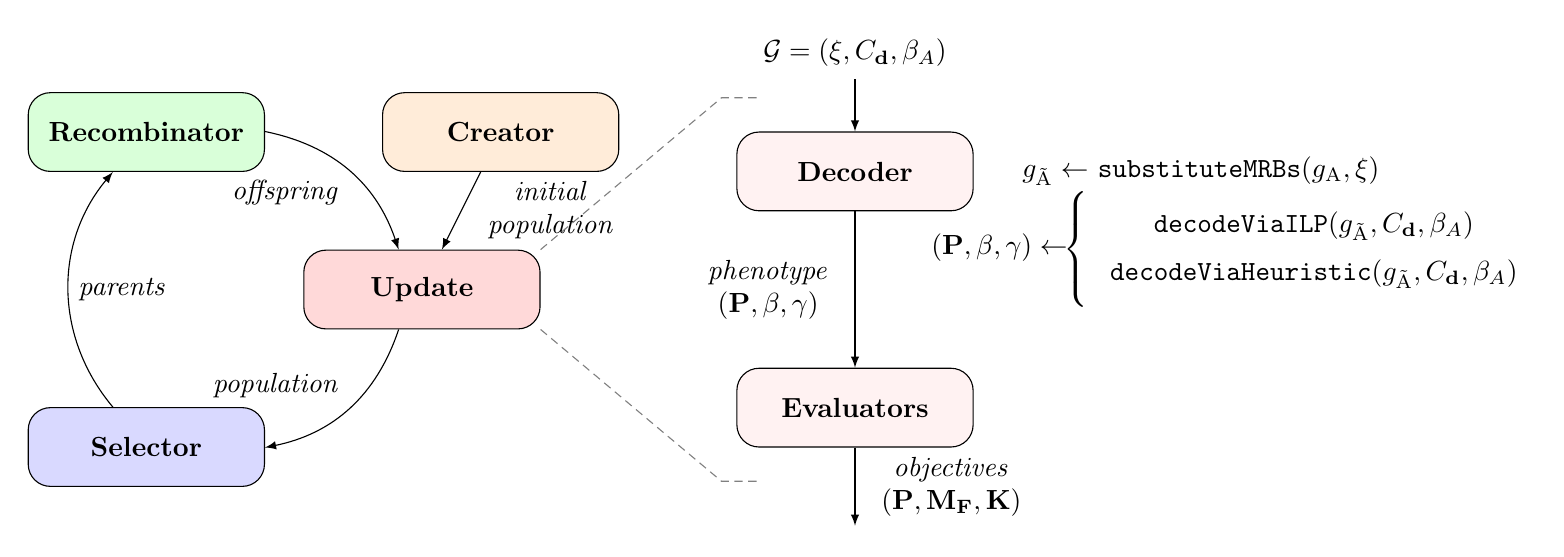
\begin{tikzpicture}
	\DesignFlow
    \end{tikzpicture}}
  \caption{\label{fig:opt4jOptimizationLoop}Overview of our hybrid DSE approach using \acp{MOEA}.
    The instance \emph{creator} generates random \emph{genotypes} for an \emph{initial population} that forms the starting point of the iterative optimization process.
    A genotype $\Genotype$ is the genetic representation of a solution candidate. % i.e., $\Genotype$. %$\GenotypeILP$ or $\GenotypeHeuristic$ in our case.
    For each (new) solution candidate, \emph{update} executes a user-defined decoder and then applies  evaluator functions on this candidate, i.e., either \texttt{decodeViaILP} or \texttt{decodeViaHeuristic}, depending on whether the \acs{ILP}-based or heuristic-based approach is used.
    The decoder transforms the genotype into the \emph{phenotype} representing the solution candidate's characteristics of interest, e.g., the period $\Period$, the bindings $\SetBindings$, and the channel capacities $\Capacity$.
    Based on the phenotype, the evaluators determine the quality of the solution candidate under evaluation with respect to the design \emph{objectives}, e.g., period $\Period$, memory footprint $\MemoryFootprint$, and core cost $\CoreCost$.
    From the resulting population, the \emph{selector} chooses \emph{parents} with superior solution quality.
    Finally, the recombinator generate \emph{offsprings} by recombining and mutating the genotype of the selected parents.
    Our approach has been realized using the \ac{DSE} framework \emph{OpenDSE}~\cite{opendse} and its underlying \acs{MOEA}-based optimization framework {\sc Opt4J}~\cite{opt4j}.}
\end{figure*}

In summary, replacing every multi-cast actor with an \ac{MRB} enables minimal memory footprint implementations, but this may create an impact on the minimal achievable period.
Thus, minimal period implementations require both optimization of the actor and channel bindings as well as a selective decision for each multi-cast actor on whether or not to perform \ac{MRB} replacement.
In the following, we present our design space exploration approach to minimize the execution period, memory footprint, and core cost.
%Our proposed \ac{DSE} explores a selective replacement of multi-cast actors by \acp{MRB} together with the bindings of actors and channels.

\section{Design Space Exploration}\label{sec:dse}

Allocation of resources, binding, and scheduling a \ac{DFG} onto a heterogeneous many-core system is a \ac{MOP}~\cite{Blickle1998,teichHSWCOUT}, and trade-offs exist and shall be explored between different objectives, e.g., execution period, memory footprint, and core cost.
In general, there is no single best solution but a set of Pareto-optimal solutions that trade the different objectives against each other.
\par
Moreover, the introduced design space of bindings and schedules is huge even for small applications and a modest number of processors, memories, and communication resources, such as the example shown in~\cref{fig:specification}.
Thus, finding the actual set of Pareto-optimal solutions is an intractable problem that can only be approximated via heuristics.
For this purpose, many state-of-the-art \ac{ESL} design flows employ \emph{meta-heuristic optimization} techniques based on \acp{MOEA}~\cite{Blickle1998,Keinert:2009,Letras:2020}.
%During this process, the optimization loop shown in~\cref{fig:opt4jOptimizationLoop} iteratively improves a population of \emph{solution candidates}.
The advantage of such population-based techniques is that the search space is sampled in parallel and that not only one compromise solution but an approximation of the Pareto-front is found after several generations of offspring as a result of the \ac{DSE}.
However, whereas \acp{MOEA} have been shown to provide quite good results for allocation and binding problems~\cite{Blickle1998,teichHSWCOUT}, it is difficult to find good encodings for feasible schedules of operations.
\par
Indeed, pure meta-heuristic optimization techniques, while applicable to a broad domain of problems, are often too generic.
This general applicability can be traded for a better optimization performance, e.g., quality of found solutions or required runtime to obtain these solutions, by employing problem-specific heuristics.
Hence, it is beneficial to \emph{integrate problem knowledge} into meta-heuristic optimization techniques -- restricting their general applicability to a particular domain but improving optimization performance.
\par
In this paper, we propose a new hybrid \ac{DSE} approach in which the exploration of the design space is split between (i) a \ac{MOEA} to explore the space of \emph{multi-cast actor replacement function} $\useMRB$ (encoded as a binary string), \emph{channel decision function} $\ChannelDecisions$ (integer encoding), and the \emph{set of actor bindings} $\SetBindingsActors$ (integer encoding).
To find a schedule minimizing the execution period $\Period$ for a given solution candidate, (ii) a specialized scheduling algorithm is applied.
This so-called hybrid \emph{decoding} process is illustrated in~\cref{fig:opt4jOptimizationLoop}.
\par
For decoding, we first propose an exact formulation for the related scheduling problem and subsequently introduce our heuristic \acs{CAPS-HMS}.
The \ac{ILP}-based decoding will obtain a schedule with minimal period for a given set of actor bindings and channel decisions but may suffer from long evaluation times.
In contrast, our heuristic \acs{CAPS-HMS} will allow for a much faster evaluation of solution candidates but does not guarantee to find the exact minimal period.
\par
In both alternative approaches, \cref{alg:merging} is applied first to compute a transformed application graph $\mrbgraph$ containing the \acp{MRB} decided by the \ac{DSE} via the multi-cast actor replacement function $\useMRB$.
This function $\useMRB$, the channel decision function $\ChannelDecisions$, and the set of actor bindings $\SetBindingsActors$ together form the genotype $\Genotype$.
In both cases, the genotype will be decoded into the \emph{phenotype} representing the period $\Period$, the set of actor and channel bindings $\SetBindings$, and the channel capacity function $\Capacity$.
Based on the phenotype, the evaluators finally determine the quality of the solution candidate under evaluation with respect to the design \emph{objectives}.
For our mapping and scheduling problem, the objectives are the minimization of
(i) the execution period $\Period$,
(ii) the memory footprint $\MemoryFootprint = \sum_{\channel \in \mrbgraph.\SetChannels} \Capacity(\channel) \cdot \Size(\channel)$, and
(iii) the core cost $\CoreCost = \sum_{\coretype \in \SetCoreTypes} \allocation(\coretype) \cdot \CoreCost_\coretype$.%
\footnote{Here, $\CoreCost_\coretype$ denotes the cost of a core of type $\coretype$.}

\section{Decoding}\label{sec:decoding}

In the following, we present and later evaluate two decoding approaches: (i) an integer linear program and (ii) a novel periodic scheduling heuristic called \acs{CAPS-HMS} for heterogeneous multi-core platforms with hierarchical memory organizations and integrating the scheduling of actors and communications between actors.

\subsection{\acs{ILP}-based Decoding}\label{sec:ILP}

First, we explain our \ac{ILP}-based decoding approach, as shown in~\cref{alg:period-via-ilp}.
This algorithm decodes the genotype $\Genotype$ into the corresponding phenotype $(\Period, \SetBindings, \Capacity)$, as shown in~\cref{fig:opt4jOptimizationLoop}.

%\LinesNotNumbered
\begin{algorithm}[htb]
  \scriptsize
  \caption{\acs{ILP}-based Decoding}\label{alg:period-via-ilp}
  \let\oldnl\nl% Store \nl in \oldnl
  \newcommand{\nonl}{\renewcommand{\nl}{\let\nl\oldnl}}%
  \SetKwProg{Fn}{Function}{}{}
  \SetKwFunction{FPeriodViaILP}{decodeViaILP}
  \SetKwInOut{Input}{Input}
  \SetKwInOut{Output}{Output}
  \SetKwRepeat{Do}{do}{while}
  \Fn{\FPeriodViaILP{$\mrbgraph, \ChannelDecisions, \SetBindingsActors$}}{
    \Input{Application graph $\mrbgraph$, channel decision function $\ChannelDecisions$, and the set of actor bindings $\SetBindingsActors$}
    \Output{Period $\Period$, set of bindings $\SetBindings$, and the channel capacity function $\Capacity$}
    \BlankLine
%   \Do{\Cref{eq:memoryConstraint} not satisfied \label{ln:ilp-loop-end}}{ \label{ln:ilp-loop-start}
    \Do{$\exists \memory \in \SetMemories : \sum_{(\channel,\memory) \in \SetBindingsChannels} \Capacity(\channel) \cdot \Size(\channel) > \MemoryCapacity{\memory}$ \label{ln:ilp-loop-end}}{ \label{ln:ilp-loop-start}
      $\SetBindingsChannels \leftarrow \texttt{determineChannelBindings}(\ChannelDecisions, \Capacity, \SetBindingsActors)$ \label{ln:ilp-derive-channel-bindings} \\
%     $\SetActors_\resource \leftarrow \{ \actor \in \mrbgraph.\SetActors \mid \resource = \SetBindingsActors(\actor) \}\quad\forall \resource \in \SetResources$\\
%     $\SetTasks_\resource \leftarrow \SetActors_\resource \cup \{ (\channel, \actor) \in \mrbgraph.\SetPGEdges \mid \resource \in \Routing(\SetBindingsActors(\actor), \SetBindingsChannels(\channel)) \}\quad\forall \resource \in \SetCores \cup \SetInterconnects$\\
%     $\SetTasks_\resource \leftarrow \SetTasks_\resource \cup \{ (\actor, \channel) \in \mrbgraph.\SetPGEdges \mid \resource \in \Routing(\SetBindingsActors(\actor), \SetBindingsChannels(\channel)) \}\quad\forall \resource \in \SetCores \cup \SetInterconnects$\\
      Solve \ac{ILP} \label{ln:ilp-solve} \\
      \nonl
        \begin{tabular}{lr@{\,}lr}
          minimize                                                                    & $\Period$                                                        & $\in \RealsNonNegative$    & \AddEqLabel{eq:ilp-objective}\\
          $\forall \task \in \SetTasks$                                               & $\startTime_\task$                                               & $\in \RealsNonNegative$    & \AddEqLabel{eq:def-start-times}\\
          $\forall (\actor, \channel), (\channel, \actor') \in \mrbgraph.\SetPGEdges$ & $\startTime_{(\actor,\channel)} + \execTime_{(\actor,\channel)} - \Period\cdot\Delay(\channel)$ & $\leq \startTime_{(\channel,\actor')}$ & \AddEqLabel{eq:dep-actor-read}\\
          $\forall (\channel,\actor) \in \mrbgraph.\SetPGEdges$                       & $\startTime_{(\channel,\actor)} + \execTime_{(\channel,\actor)}$ & $\leq \startTime_\actor$   & \AddEqLabel{eq:dep-actor-execute}\\
          $\forall (\actor,\channel) \in \mrbgraph.\SetPGEdges$                       & $\startTime_\actor + \execTime_\actor$                           & $\leq \startTime_{(\actor,\channel)}$                                 & \AddEqLabel{eq:dep-actor-write}\\
          $\forall \resource \in \SetResources\;\forall \task, \task' \in \SetTasks_\resource$ & $\startTime_\task + \execTime_\task - \Period$          & $\leq \startTime_{\task'}$ & \AddEqLabel{eq:cstr-resource}\\
        \multicolumn{2}{l@{\,}}{$\forall \resource \in \SetInterconnects \cup \SetCores\;\forall \task, \task' \in \SetTasks_\resource \wedge \task \neq \task'$\hspace{1.7cm}$\order_{\task,\task'}$}
                                                            & $\in \{0, 1\}$                              & \AddEqLabel{eq:def-order-edges}\\
          & $\order_{\task,\task'} + \order_{\task',\task}$ & $= 1$                                       & \AddEqLabel{eq:cstr-order-one}\\
        \multicolumn{4}{l}{$\forall \interconnect \in \SetInterconnects\;\forall \task, \task' \in \SetTasks_\interconnect \wedge \task \neq \task'$}\\
          & $\startTime_\task + \execTime_\task - \bigDelay\cdot(1-\order_{\task,\task'})$                & $\leq \startTime_{\task'}$ & \AddEqLabel{eq:seq-communicate}\\
        \multicolumn{4}{l}{$\forall \core \in \SetCores\;\forall \actor, \actor' \in \SetActors_\core \wedge \actor \neq \actor'\;\forall \task \in OUT(\actor), \task' \in IN(\actor')$}\\
          & $\startTime_\task + \execTime_\task - \bigDelay\cdot(1-\order_{\actor,\actor'})$              & $\leq \startTime_{\task'}$ & \AddEqLabel{eq:seq-compute}
        \end{tabular}\nl\\
      Increase $\Capacity(\channel)$ to accommodate \ac{ILP} schedule \quad$\forall \channel \in \mrbgraph.\SetChannels$ \label{ln:ilp-increase-channel-capacities}\\
    }
    \Return $(\Period, \SetBindingsActors \cup \SetBindingsChannels, \Capacity)$
  }
\end{algorithm}
%\LinesNumbered
Note that the scheduling via \ac{ILP} is performed in a loop (\crefrange{ln:ilp-loop-start}{ln:ilp-loop-end}).
The reason is that for an \ac{ILP}-derived schedule, the channel capacities might need to be increased to execute this schedule (\cref{ln:ilp-increase-channel-capacities}), and the channel bindings might need to be modified in consequence to accommodate the enlarged channels (\cref{ln:ilp-derive-channel-bindings}).
The loop terminates when all channels fit into the memories they are bound to (\cref{ln:ilp-loop-end}).
\par
The objective of the \ac{ILP} itself is the minimization of the execution period $\Period$ (\cref{eq:ilp-objective}).
Moreover, for each task $\task \in \SetTasks$, the \ac{ILP} determines a start time $\startTime_\task$ (\cref{eq:def-start-times}).
\Crefrange{eq:dep-actor-read}{eq:dep-actor-write} encode the data dependencies of the application graph $\mrbgraph$.
In particular, \cref{eq:dep-actor-read} denotes that a token cannot be read from a channel $\channel$ before it has been written into it, also considering the number of initial tokens $\Delay(\channel)$ of the channel.
\Cref{eq:dep-actor-execute} ensures that each actor can only start after all its reads from ingoing edges have been performed, and \cref{eq:dep-actor-write} enforces that each actor write can only start after its actor computation has finished.
\Cref{eq:cstr-resource} guarantees for each resource $\resource$ that all tasks $\task \in \SetTasks_\resource$ mapped to this resource are executed within a time interval of duration $\Period$.
Finally, to ensure a feasible schedule, the \ac{ILP} must enforce that tasks mapped to the same resource have non-overlapping executions.
For this purpose, sequentialization binary variables $\order_{\task,\task'}$ are introduced for each pair of tasks that share a resource (\cref{eq:def-order-edges}).
Here, $\order_{\task,\task'} = 1$ denotes that task $\task$ must finish before task $\task'$ is started.
Thus, exactly either $\order_{\task,\task'}$ or $\order_{\task',\task}$ must be one (\cref{eq:cstr-order-one}).
These variables are then used to sequentialize the communication over the interconnects (\cref{eq:seq-communicate}) and the actor executions performed by the cores (\cref{eq:seq-compute}).
In these equations, $\bigDelay \gg \Period$ is a value much greater than the execution period, that is used to disable the sequentialization constraint that task $\task$ must finish before task $\task'$ is started in the case that $\order_{\task,\task'} = 0$.
The sequentialization of actors mapped to the same core (\cref{eq:seq-compute}) is enforced indirectly by constraining that all write tasks $\task \in OUT(\actor)$ of actor $\actor$ are finished before the read tasks $\task' \in IN(\actor')$ of actor $\actor'$ are started.
This ensures that all reads of an actor, then the actor itself, and finally, all writes of the actor are executed in sequence without interspersing of reads and writes of other actors into this sequence.
\par
However, if actor $\actor$ is a sink actor (i.e., has no output edges) or actor $\actor'$ is a source actor (i.e., has no input edges), a simple definition of $OUT(\actor)$ and $IN(\actor')$ as the set of all output edges of actor $\actor$, respectively, the set of all input edges of actor $\actor'$ would fail to enforce the sequentialization that actor $\actor$ is completed before actor $\actor'$ fires.
To handle these cases, $OUT(\actor)$ returns the set containing only the actor $\actor$ itself when this actor is a sink.
Conversely, $IN(\actor')$ returns the set containing only the actor $\actor'$ itself when this actor is a source.
Formally, $OUT(\actor)$ and $IN(\actor')$ are defined as follows:
\scalebox{0.86}{\parbox{1.14\columnwidth}{
\begin{align*}
  OUT(\actor) = & \begin{cases}
       \SetPGEdgesOut(\actor) & \text{if } \SetPGEdgesOut(\actor) \neq \emptyset \\
       \{ \actor \}           & \text{otherwise}
    \end{cases}&
  IN(\actor') = & \begin{cases}
       \SetPGEdgesIn(\actor') & \text{if } \SetPGEdgesIn(\actor') \neq \emptyset \\
       \{ \actor' \}          & \text{otherwise}
    \end{cases}
\end{align*}}}
Here, $\SetPGEdgesOut(\actor) = \{ (\hat{\actor}, \hat{\channel}) \in \mrbgraph.\SetPGEdgesOut \mid \hat{\actor} = \actor \}$ denotes the set of all output edges (i.e., write operations) of actor $\actor$ and, correspondingly, $\SetPGEdgesIn(\actor') = \{ (\hat{\channel}, \hat{\actor}) \in \mrbgraph.\SetPGEdgesIn \mid \hat{\actor} = \actor' \}$ denotes the set of all input edges (i.e., read operations) of actor $\actor'$.

\subsection{Heuristic-based Decoding}\label{sec:heuristic}

\begin{figure*}[ht]
%  \begin{subfigure}[b]{\textwidth}
  \resizebox{1.02\textwidth}{!}{
  \begin{tikzpicture}
     \ExampleHeuristic
  \end{tikzpicture}
  }
  \caption{\label{fig:exHeuristicOne} Left: Example of given actor and channel bindings, with all communication channels bound to $\memory_{\tile_1}$, actors $\actor_1$ and $\actor_2$ bound to core $\core_1$, and actors $\actor_3$, $\actor_4$, and $\actor_5$ bound to cores $\core_2$, $\core_3$, and $\core_4$, respectively.
    During scheduling, time intervals in the utilization sets $\Utilization_\resource$ are allocated to task executions, e.g., in the partial schedule depicted in the middle, the execution of actor $\actor_1$ is allocating the time interval $[0,2[ \subseteq \Utilization_{\core_1}$ in the utilization set of core $\core_1$.
    This partial schedule represents the state when the actors $\actor_1$, $\actor_2$, and $\actor_3$ and all their read and write operations have already been scheduled, and the heuristic is trying to schedule actor $\actor_4$ with its read and write operations.
    In this state, the read $(\channel_3,\actor_4)$, execute (actor $\actor_4$), and write $(\actor_4,\channel_5)$ sequence has to be delayed from $7$ to $10$ due to contention in the interconnect $\crossbar{1}$, i.e., the interconnect is already occupied by the read $(\channel_2,\actor_3)$ and the write $(\actor_3,\channel_4)$.
    The final schedule is depicted on the right, where all actors and their read and write operations are shown in the schedule interval $[0, 10[$.
    Note that the depicted tasks are from different iterations, e.g., the execution of actor $\actor_4$ is from one iteration in the past, while the execution of actor $\actor_5$ is from two iterations in the past.}
\end{figure*}

To speed up evaluation during exploration, we propose an alternative heuristic-based decoding outlined in~\cref{alg:period-via-heuristic}.
%for finding periodic schedules for marked graphs using the heuristic-based decoding outlined in~\cref{alg:period-via-heuristic}.
This algorithm decodes the input genotype $\Genotype$ into the corresponding phenotype $(\Period, \SetBindings, \Capacity)$, as shown in \cref{fig:opt4jOptimizationLoop}.
\par
\begin{algorithm}[t!]
  \scriptsize
  \caption{Heuristic-based Decoding}\label{alg:period-via-heuristic}
  \SetKwRepeat{Do}{do}{while}
  \SetKwFunction{FindPeriod}{decodeViaHeuristic}
  \SetKw{False}{false}
  \SetKw{True}{true}
  \SetKw{Break}{break}
  \SetKw{Continue}{continue}
  \SetKwInOut{Input}{Input}
  \SetKwInOut{Output}{Output}
  \SetKwProg{Fn}{Function}{}{}
  \Fn{\FindPeriod{$\mrbgraph, \ChannelDecisions, \SetBindingsActors$}}{
    \Input{Application graph $\mrbgraph$, channel decision function $\ChannelDecisions$, and the set of actor bindings $\SetBindingsActors$}
    \Output{Period $\Period$, set of bindings $\SetBindings$, and the channel capacity function $\Capacity$}
    $\SetBindingsChannels \leftarrow \texttt{determineChannelBindings}(\ChannelDecisions, \Capacity, \SetBindingsActors)$\label{ln:heuristic-initial-channel-bindings}\\
    $\Period \leftarrow  \max\limits_{\forall \resource \in \SetCores \cup \SetInterconnects} \Big\lceil \sum\limits_{ \forall \task \in \SetTasks_\resource} \execTime_\task \Big\rceil $ \label{ln:heuristic-MII}\\
    \While{\True\label{ln:heuristic-remap-loop-begin}}{
      \While{$\neg\canSchedule(\mrbgraph,\SetBindingsActors,\SetBindingsChannels,\Period)$\label{ln:heuristic-schedule-loop-begin}}{
        $\Period \leftarrow \Period + 1$\label{ln:heuristic-schedule-loop-end}}
      Increase $\Capacity(\channel)$ to accommodate schedule \quad$\forall \channel \in \mrbgraph.\SetChannels$\label{ln:heuristic-increase-channel-capacities}\\
      \If{$\forall \memory \in \SetMemories : \sum_{(\channel,\memory) \in \SetBindingsChannels} \Capacity(\channel) \cdot \Size(\channel) \leq \MemoryCapacity{\memory}$\label{ln:heuristic-check-memory-capacities}}{
        \Break\label{ln:heuristic-remap-loop-terminate}}
      $\SetBindingsChannels \leftarrow \texttt{determineChannelBindings}(\ChannelDecisions, \Capacity, \SetBindingsActors)$\label{ln:heuristic-update-channel-bindings}\label{ln:heuristic-remap-loop-end}}
    \Return $(\Period,\SetBindingsActors \cup \SetBindingsChannels, \Capacity)$\label{ln:heuristic-return-phenotype}
  }
\end{algorithm}
First, we determine an initial set of channel bindings $\SetBindingsChannels$ in~\cref{ln:heuristic-initial-channel-bindings}.
Note that channels may need to be remapped later on (\cref{ln:heuristic-update-channel-bindings}) if it turns out that channel capacities need to be increased (\cref{ln:heuristic-increase-channel-capacities}) to accommodate the found schedule and at least one channel no longer fits into the memory it is bound to (checked in~\cref{ln:heuristic-check-memory-capacities}).
After initial channel bindings have been determined in \cref{ln:heuristic-initial-channel-bindings}, a lower bound for the period $\Period$ is derived in~\cref{ln:heuristic-MII} from the resource utilization of cores and interconnects.
Consider \cref{fig:exHeuristicOne} as an example, where bindings and timings are chosen for illustrative purposes with a communication time of one for all reads and writes, i.e., $\execTime_\task = 1\;\forall \task \in \SetPGEdges$.
The bottleneck resource in this example is the crossbar $\crossbar{1}$ involved in five reads and five writes, leading to a lower bound of $10$ for the period $\Period$.
\par
A concrete schedule is calculated by the proposed scheduler \revised{\ac{CAPS-HMS}} depicted in~\cref{alg:canSchedule}.
\ac{CAPS-HMS} is called with an application $\mrbgraph$, actor and channels bindings $\SetBindingsActors$ and $\SetBindingsChannels$, and a candidate period $\Period$.
If a schedule with period $\Period$ is found, \textbf{true} is returned, \textbf{false} otherwise.
This is used by the loop in~\crefrange{ln:heuristic-schedule-loop-begin}{ln:heuristic-schedule-loop-end} of~\cref{alg:period-via-heuristic} to successively increase the period until a schedule is found.
As discussed previously, channel capacities may need to be enlarged to accommodate the found schedule, possibly resulting in a need to remap channels no longer fitting into memory, necessitating a rescheduling with the updated channel bindings, as is done by the while loop in~\crefrange{ln:heuristic-remap-loop-begin}{ln:heuristic-remap-loop-end}.
Otherwise, as soon as a schedule with a feasible period $\Period$ is found and all channels fit into the memory they are bound to, \cref{ln:heuristic-remap-loop-terminate} terminates the loop.
Then, the resulting phenotype $(\Period, \SetBindings, \Capacity)$ is returned in~\cref{ln:heuristic-return-phenotype}.
\par
$\canSchedule$ shown in~\cref{alg:canSchedule} follows a greedy strategy, where tasks are scheduled as soon as possible on the resources they are bound to.
All tasks are assigned a start time of execution within a given interval $[0, \Period[$, i.e., from 0 (included) to $\Period$ (excluded).
Ultimately, this interval will contain tasks from different iterations to optimize resource utilization.
To obtain a schedule within the interval $[0, \Period[$, \acs{CAPS-HMS} schedules one iteration of the application graph $\mrbgraph$, thereby wrapping task executions finishing later than the period $\Period$ back into the \emph{schedule interval} $[0, \Period[$ through modulo $\Period$ computation.
Assuming the task $\task$ is executed in the interval $[\startTime_\task, \startTime_\task + \execTime_\task[$, then in the schedule interval $[0, \Period[$, it will occupy the time region given by $\fWrap(\Period,\startTime_\task, \execTime_\task) = \{ t\mod\Period \mid \startTime_\task \leq t < \startTime_\task + \execTime_\task \}$.
For example, the execution of actor $\actor_3$ in the schedule depicted in~\cref{fig:exHeuristicOne} (to the right) is from 8 to 11, but it is wrapped into the schedule interval $[0, 10[$ with $\fWrap(10,8,3) = [8, 10[ \cup [0, 1[$.
\par
During scheduling, the \emph{resource utilization} of each core or interconnect resource $\resource \in \SetResources \setminus \SetMemories$ is tracked by a corresponding utilization set $\Utilization_\resource \subseteq [0,\Period[$ that contains all time intervals already occupied with scheduled tasks.
Initially, all resources are free, i.e., the utilization sets are assigned the empty set (\cref{ln:heuristic-clear-utilization-sets} in~\cref{alg:canSchedule}).
For example, in the state depicted by the partial schedule shown in the middle of~\cref{fig:exHeuristicOne}, the actors $\actor_1$, $\actor_2$, and $\actor_3$ and all their read and write operations have already been scheduled.
In this state, the heuristic is trying to schedule actor $\actor_4$ with its read and write operations, observing the utilization sets $\Utilization_\crossbar{1} = [1,4[ \cup [5,8[$, $\Utilization_{\core_1} = [0,7[$, $\Utilization_{\core_2} = [0,2[ \cup [7,10[$, $\Utilization_{\core_3} = \Utilization_{\core_4} = \emptyset$.
\par
The goal of the scheduling heuristic $\canSchedule$ is to assign for each task $\task \in \SetTasks$ a as early as possible start time $\startTime_\task$ that conforms with the given bindings and satisfies the data dependencies.
Channel capacities are not considered during scheduling but are adjusted in~\cref{alg:period-via-heuristic} to accommodate the found schedule.
The start times are initialized with zero at algorithm start (\cref{ln:heuristic-zero-start-times} in~\cref{alg:canSchedule}) as, later on, the heuristic only delays start times to conform to data dependencies and resource constraints.
$\fHeuristic$ considers for each actor a priority given by the topological sorting of $\mrbgraph$ (see \cref{ln:priority}).
During scheduling, the heuristic keeps track of actors to be scheduled with the list $\ReadyList$ of ready actors, which is initialized in~\cref{ln:heuristic-init-readylist} as all actors that are initially ready to be fired, e.g., because they are source actors or there is at least one initial token contained in all input channels of the actor.
Before any actor is selected, the ready list $\ReadyList$ must be sorted in descending order using the previously assigned priority.
%To schedule the actors, we use a ready list $\ReadyList$ to track the set of fireable actors.
%When the ready list $\ReadyList$ is empty, it means that all the actors have been successfully scheduled (see \cref{algH:stop}).
\par
Actor scheduling is performed by the loop in~\crefrange{ln:heuristic-begin-schedule-loop}{ln:heuristic-end-schedule-loop}, which either \emph{succeeds} (\cref{ln:heuristic-schedule-success}) when there are no longer any actors to be scheduled, i.e., $\ReadyList = \emptyset$, or \emph{fails} (\cref{ln:heuristic-schedule-failure}) when an actor can not be scheduled within the schedule interval $[0, \Period[$ due to insufficient free time remaining on at least one resource to schedule the actor and its read and write operations.
This failure is indicated by the error flag $\varpi$ checked in (\cref{ln:heuristic-check-failure}).
Within the scheduling loop, an actor $\actor$ to be scheduled is selected from the ready list $\ReadyList$, and its core $\core$ onto which it is bound is derived from the bindings $\SetBindingsActors$ (\cref{ln:heuristic-select-actor}).
Then, the time $\execTime'_\actor$ that an actor $\actor$, including its communication tasks, requires to be scheduled on core $\core$ is computed.
For this purpose, we sum the actor’s execution time $\execTime_{\actor}$ and the required times $\timeInputReads$ and $\timeOutputWrites$ for the actors read $\task \in \SetPGEdgesIn(\actor)$ and write $\task \in \SetPGEdgesOut(\actor)$ communication tasks (see \cref{ln:heuristic-actor-com-plus-exec-time}).
To exemplify, for the actor $\actor_1$, $\execTime_{\SetPGEdgesIn(\actor_1)} = 0$ as the actor is a source actor having no inputs, $\execTime_{\SetPGEdgesOut(\actor_1)} = 1$ as there is a single write task with communication time $\execTime_{(\actor_1,\channel_1)} = 1$, resulting in an overall time including communication of $\execTime'_{\actor_1} = \execTime_{\SetPGEdgesIn(\actor_1)} + \execTime_{\actor_1} + \execTime_{\SetPGEdgesOut(\actor_1)} = 0 + 2 + 1 = 3$.
\par
\begin{algorithm}[t!]
  \scriptsize
  \caption{$\fHeuristic$}\label{alg:canSchedule}
  \SetKwRepeat{Do}{do}{while}
  \SetKwFunction{FMain}{$\canSchedule$}
  \SetKw{Continue}{continue}
  \SetKw{False}{false}
  \SetKw{True}{true}
  \SetKw{Break}{break}
  \SetKwInOut{Input}{Input}
  \SetKwInOut{Output}{Output}
  \SetKwProg{Fn}{Function}{}{}
  \SetKwFor{Case}{case}{}{end case}%

  \Fn{\FMain{$\mrbgraph, \SetBindingsActors, \SetBindingsChannels, \Period$}}{
    \Input{Application $\mrbgraph$, bindings $\SetBindingsActors$ and $\SetBindingsChannels$, and a candidate period $\Period$ }
    \Output{\True if a schedule for $\mrbgraph$ of period $\Period$ is found, \False otherwise}
    \parbox{1cm}{$\Utilization_{\resource}  \leftarrow \emptyset$}$\forall \resource \in \SetResources \setminus \SetMemories$ \label{ln:heuristic-clear-utilization-sets} \\
    \parbox{1cm}{$\startTime_\task          \leftarrow 0        $}$\forall \task \in \SetTasks = \mrbgraph.\SetActors \cup \mrbgraph.\SetPGEdges$ \label{ln:heuristic-zero-start-times} \\
    $z_{\actor}\leftarrow $ assign  topological sorting~\cite{cormen} as priority $\forall \actor \in \mrbgraph.\SetActors$\label{ln:priority} \\
    $\ReadyList \leftarrow \{\actor \in \mrbgraph.\SetActors \mid \actor\textrm{ is ready to fire }\}$ \label{ln:heuristic-init-readylist}\\
    \While{$\ReadyList \neq \emptyset$\label{ln:heuristic-begin-schedule-loop}}{
      Sort $\ReadyList$ in descending order using priority $z$ \label{ln:sort} \\
      $\actor \leftarrow \fPop(\ReadyList)$ ; $\core \leftarrow \SetBindingsActors(\actor)$ \label{ln:heuristic-select-actor} \\
    $\timeInputReads \leftarrow \sum\limits_{\task \in \SetPGEdgesIn(\actor)} \execTime_{\task}$ ; $\timeOutputWrites \leftarrow \sum\limits_{\task \in \SetPGEdgesOut(\actor)} \execTime_{\task}$ ; $\execTime'_\actor \leftarrow \timeInputReads + \execTime_\actor + \timeOutputWrites$ \label{ln:heuristic-actor-com-plus-exec-time} \\
      $\varpi \leftarrow \True$ \label{ln:heuristic-init-error-indicator} \\
      \ForEach{$\startTime'_\actor \in [\startTime_\actor,\startTime_\actor+\Period[: \Utilization_\core \cap \fWrap(\Period, \startTime'_\actor, \execTime'_\actor) = \emptyset$\label{ln:heuristic-free-core-time-span}
 }{
        \parbox{2.6cm}{$(\task_{cns,1},\task_{cns,2},\ldots\task_{cns,|\SetPGEdgesIn(\actor)|})$}  $\leftarrow \SetPGEdgesIn(\actor)$\label{ln:heuristic-order-inputs}\\
        \parbox{2.6cm}{$(\task_{prd,1},\task_{prd,2},\ldots\task_{prd,|\SetPGEdgesOut(\actor)|})$} $\leftarrow \SetPGEdgesOut(\actor)$\label{ln:heuristic-order-outputs}\\
        \parbox{2.3cm}{$\startTime_{\task_{cns,i}} \leftarrow \startTime'_\actor                                     $}$ + \sum\limits_{j=1}^{i-1} \execTime_{\task_{cns,j}}\quad\forall i \in \{1,\ldots,|\SetPGEdgesIn(\actor)|\}$  \label{ln:heuristic-assign-read-times} \\
        \parbox{2.3cm}{$\startTime_{\task_{prd,i}} \leftarrow \startTime'_\actor + \timeInputReads + \execTime_\actor$}$ + \sum\limits_{j=1}^{i-1} \execTime_{\task_{prd,j}}\quad\forall i \in \{1,\ldots,|\SetPGEdgesOut(\actor)|\}$ \label{ln:heuristic-assign-write-times} \\
	\If{$\forall \task \in \SetPGEdgesIn(\actor) \cup \SetPGEdgesOut(\actor), \resource \in \Routing(\task) : \Utilization_\resource \cap \fWrap(\Period, \startTime_\task, \execTime_\task) = \emptyset$ \label{ln:heuristic-free-interconnects}}{
                $\startTime_\actor \leftarrow \startTime'_\actor +\timeInputReads $ \label{ln:heuristic-update-actor-start-time}\\
		$\Utilization_\core     \leftarrow \Utilization_\core     \cup \fWrap(\Period, \startTime_\actor,\execTime_\actor)$ \label{ln:heuristic-schedule-actor} \\
		\parbox{2.5cm}{$\Utilization_\resource \leftarrow \Utilization_\resource \cup \fWrap(\Period, \startTime_\task, \execTime_\task)$} $\forall \task \in \SetPGEdgesIn(\actor) \cup \SetPGEdgesOut(\actor), \resource \in \Routing(\task)$ \label{ln:heuristic-schedule-com} \\
                \parbox{2.5cm}{$\startTime_{\actor'} \leftarrow \max(\startTime_{\actor'}, \startTime'_\actor + \execTime'_{\actor})$}             $\forall (\actor,\channel), (\channel,\actor') \in \mrbgraph.\SetPGEdges \wedge \Delay(\channel) = 0$ \label{ln:heuristic-update-successor-start-times} \\
                $\ReadyList \leftarrow (\ReadyList \setminus \{\actor\}) \cup \{\actor' \in \mrbgraph.\SetActors \mid \textrm{unscheduled actor }\actor'$ is ready due to the firing of actor $\actor\}$\label{ln:heuristic-update-readylist}\\
                $\varpi \leftarrow \False$ ; \Break \label{ln:heuristic-clear-error-indicator}
        }
      }
      \If{$\varpi$\label{ln:heuristic-check-failure}}{
	\Return \False \label{ln:heuristic-schedule-failure}}\label{ln:heuristic-end-schedule-loop}
    }
    \Return \True \label{ln:heuristic-schedule-success}
  }
\end{algorithm}
Next, the scheduling heuristics searches for a free time span $[\startTime'_\actor, \startTime'_\actor+\execTime'_\actor[$ in the utilization set $\Utilization_\core$ of core $\core$ (\cref{ln:heuristic-free-core-time-span}) to schedule the actor $\actor$ and its read and write operations.
First, however, the error indicator $\varpi$ is set to \textbf{true} (\cref{ln:heuristic-init-error-indicator}).
Later, in case the loop in~\crefrange{ln:heuristic-free-core-time-span}{ln:heuristic-clear-error-indicator} successfully schedules the actor and its communication, the error flag $\varpi$ will be reset to \textbf{false} to indicate success, and the loop will be terminated (\cref{ln:heuristic-clear-error-indicator}).
In detail, \cref{ln:heuristic-free-core-time-span} iterates over start times $\startTime'_\actor$ that satisfies the data dependencies of actor $\actor$, i.e., $\startTime'_\actor \geq \startTime_\actor$, while simultaneously not overlapping with already scheduled tasks on core $\core$, i.e., $\Utilization_\core \cap \fWrap(\Period, \startTime'_\actor, \execTime'_\actor) = \emptyset$.
Moreover, as the schedule is $\Period$ periodic, the heuristic only needs to examine start times $\startTime'_\actor < \startTime_\actor + \Period$.
\par
Next, the read $\task_{cns,i}$ and write $\task_{prd,i}$ operations of actor $\actor$ are identified in~\cref{ln:heuristic-order-inputs,ln:heuristic-order-outputs}.
Then, for each read $\task_{cns,i}$ operation, a start time $\startTime_{\task_{cns,i}}$ is assigned from the time span $[\startTime'_{\actor}, \startTime'_{\actor}+\timeInputReads[$ before the execution of actor $\actor$ (see \cref{ln:heuristic-assign-read-times}).
Conversely, for each write task $\task_{prd,i}$, a start time $\startTime_{\task_{prd,i}}$ is assigned from the time span $[\startTime'_{\actor}+\timeInputReads+\execTime_\actor,\startTime'_{\actor}+\execTime'_\actor[$ just after the execution of actor $\actor$ (see \cref{ln:heuristic-assign-write-times}).
Subsequently, $\canSchedule$ checks for each communication task $\task \in \SetPGEdgesIn(\actor) \cup \SetPGEdgesOut(\actor)$ if all the (interconnect) resources $\resource \in \Routing(\task)$ traversed by the read or write operation $\task$ are available during the time span $[\startTime_\task,\startTime_\task+\execTime_\task[$ in which the communication operation is performed (\cref{ln:heuristic-free-interconnects}).
If the interconnects are free, the start time of actor $\actor$ is updated (see \cref{ln:heuristic-update-actor-start-time}), actor $\actor$ is scheduled to core $\core$ (see \cref{ln:heuristic-schedule-actor}), and each communication task $\task \in \SetPGEdgesIn(\actor) \cup \SetPGEdgesOut(\actor)$ is scheduled to its traversed resources $\resource \in \Routing(\task)$ (see \cref{ln:heuristic-schedule-com}).
Then, for each successor actor $\actor'$ of actor $\actor$, its start time $\startTime_{\actor'}$ is updated to respect the data dependency between actor $\actor$ and $\actor'$ (\cref{ln:heuristic-update-successor-start-times}).
Next, actor $\actor$ is removed from the ready list $\ReadyList$, and all unscheduled actors $\actor'$ that have been enabled by firing actor $\actor$ are added to the ready list (\cref{ln:heuristic-update-readylist}).
Finally, the foreach loop is terminated in~\cref{ln:heuristic-clear-error-indicator} to continue scheduling the next actor until all the actors have been scheduled (\cref{ln:heuristic-schedule-success}) or there is insufficient free time remaining on at least one resource to schedule all actors and their read and write operations (\cref{ln:heuristic-schedule-failure}).
\par
\revised{The complexity of the \ac{CAPS-HMS} heuristic can be derived from analyzing the nested loops in \cref{ln:heuristic-begin-schedule-loop,ln:heuristic-free-core-time-span,ln:heuristic-free-interconnects}.
The outer while loop in~\cref{ln:heuristic-begin-schedule-loop}, which iterates over all tasks $\task \in \SetTasks$ to be scheduled, contributes to the overall complexity of~\cref{alg:canSchedule} with a factor of $|\SetTasks|$, with $\SetTasks = \SetActors \cup \SetPGEdges$.
The foreach loop in~\cref{ln:heuristic-free-core-time-span} contributes to the overall complexity of~\cref{alg:canSchedule} also with a factor of $|\SetTasks|$, as we need to check at most $|\SetTasks|$ points in time.
Finally, the impact of the iteration over all resources $\resource \in \Routing(\task)$ traversed by a communication task $\task$ of actor $\actor$ (see the if condition in~\cref{ln:heuristic-free-interconnects}) depends on the number of traversed resources limited by the number of interconnects $|\SetInterconnects|$, and to account also for the core the actor is bound to, this number increases by one, i.e., $|\SetInterconnects|+1$.
In summary, the complexity of \ac{CAPS-HMS} is therefore $O(|\SetTasks|^2\cdot(|\SetInterconnects|+1))$, which is polynomial w.r.t. the number of tasks $|\SetTasks|$ to be scheduled.}
%\revised{The complexity of the \ac{CAPS-HMS} heuristic can be derived from analyzing the nested loops in \cref{ln:heuristic-begin-schedule-loop,ln:heuristic-free-core-time-span,ln:heuristic-free-interconnects}. 
%The expression in \cref{ln:heuristic-free-interconnects} represents a loop that iterates over both all edges (i.e., communication tasks $\task \in \SetPGEdgesIn(\actor)  \cup \SetPGEdgesOut(\actor)$) adjacent to actor $\actor$ and resources $\resource \in \Routing(\task)$ traversed by these communication tasks to check the if condition. 
%Note that iterating over all adjacent edges to actor $\actor$ is also performed in \cref{ln:heuristic-actor-com-plus-exec-time,ln:heuristic-order-inputs,ln:heuristic-order-outputs,ln:heuristic-assign-read-times,ln:heuristic-assign-write-times,ln:heuristic-schedule-com,ln:heuristic-update-successor-start-times}. 
%The complexity contribution of the iteration over all adjacent edges of an actor $\actor$ can be factored out by observing that all edges $\edge \in \SetPGEdges$ of $\mrbgraph$ will be iterated over when we have iterated over all actors $\actor \in \SetActors$ of $\mrbgraph$. 
%The outer while loop in \cref{ln:heuristic-begin-schedule-loop}, which iterates over all actors, contributes to the overall complexity of \cref{alg:canSchedule} with a factor of $|\SetTasks|$, as $\SetTasks = \SetActors \cup \SetPGEdges$. 
%Next, the complexity factor contribution of the loop in \cref{ln:heuristic-free-core-time-span} is examined. 
%First, note that the loop searches for the earliest time an actor and its communication tasks can start. 
%Therefore, the actor or at least one of its communication tasks will start immediately after another task has finished. 
%The foreach loop in \cref{ln:heuristic-free-core-time-span} contributes to the overall complexity of \cref{alg:canSchedule} with a factor of $|\SetTasks|$, as we need to check at most $|\SetTasks|$ points in time. 
%Finally, the impact of the iteration over all resources $\resource \in \Routing(\task)$ traversed by a communication task $\task$ of actor $\actor$ (see the if condition in \cref{ln:heuristic-free-interconnects}) depends on the number of traversed resources limited by the number of interconnects $|\SetInterconnects|$, and to account for the core the actor is bound to, this number has to be increased by one, i.e., $|\SetInterconnects|+1$. 
%In summary, the complexity of \ac{CAPS-HMS} is $O(|\SetTasks|^2\cdot(|\SetInterconnects|+1))$, which is polynomial w.r.t. the number of tasks $|\SetTasks|$ to be scheduled.
%}
%\revised{In summary, the complexity of \ac{CAPS-HMS} is $O((|\SetTasks|)^2)$ which is polynomial w.r.t. the number of tasks $|\SetTasks|$ to be scheduled.
%In a worst case, the number of operations to be executed by \cref{alg:canSchedule} are $|\SetTasks|$ tasks to be scheduled times the number of possible gaps in the utilization list $\Utilization$ that might also be $|\SetTasks|$ at most.
%}
\par
We will see in~\cref{sec:results} that although our heuristic scheduler $\canSchedule$ does not guarantee to determine a schedule of minimal period $\Period$ for a given combination of graph, channel decision function, and actor bindings, it turns out to require much less execution time than using the \ac{ILP} scheduling approach presented in \cref{sec:ILP}.
When comparing related Pareto front qualities, we will also show that the degradation is little for many test applications.
Particularly for large applications and complexity of the target architecture, the \ac{ILP} solution times can become prohibitively long.

\vspace{-1mm}
\section{Results}\label{sec:results}

In the following, we conduct a series of different \ac{DSE} experiments as shown in~\cref{fig:opt4jOptimizationLoop} to assess the effectiveness of our proposed \ac{ILP} and \ac{CAPS-HMS} heuristic in generating high-quality implementations when mapping dataflow applications onto the heterogeneous many-cores shown in~\cref{fig:specification}.
For each exploration, we employed the OpenDSE~\cite{opendse} framework using the NGSA-II elitist genetic algorithm~\cite{dpam_2002-nsgaII} with a population size of $100$ individuals, each generation generating $25$ new individuals and the crossover rate set to $0.95$.
\revised{Since the presented \ac{ILP} and \ac{CAPS-HMS} are implemented as evaluators in OpenDSE, they have both been implemented using the Java programming language.
In the case of the proposed \ac{ILP} approach, the solver used to solve the constraints is CPLEX~\cite{cplex2024}. 
The platform used to run \ac{DSE} is a 4-core Intel(R) Core(TM) i7-4790 running at 3.60 GHz with 32 GB of  RAM.}
To measure the effects of selectively introducing \acp{MRB}, we implemented and compared three different exploration strategies: $\Reference$, $\MergingAlways$, and $\MergingExplore$.
The genotype for the $\Reference$ strategy is $\Genotype = (\ChannelDecisions, \SetBindingsActors)$.
The multi-cast actor replacement function $\useMRB$ is the all-zeros function.
Thus, no multi-cast actor is replaced (i.e., $\mrbgraph=\pgraph$).
In contrast, $\MergingAlways$ also uses the genotype $\Genotype = (\ChannelDecisions, \SetBindingsActors)$ but assumes the all-ones function for $\useMRB$.
Thus, each multi-cast actor is replaced by its corresponding \ac{MRB}.
Finally, strategy $\MergingExplore$ selectively explores for each multi-cast actor the choice of its replacement by an \ac{MRB} by using the complete genotype $\Genotype = (\useMRB, \ChannelDecisions, \SetBindingsActors)$.
Here, the binary string $\useMRB$ is determined during the optimization loop (see \cref{fig:opt4jOptimizationLoop}).
\par
Orthogonal to the replacement of multi-cast actors by \acp{MRB}, we also decide on decoding the genotype of each implementation.
Here, we observe the effects of decoding via an ILP (see \cref{sec:ILP}) or using \ac{CAPS-HMS} (see \cref{sec:heuristic}).
Both return a phenotype $(\Period,\MemoryFootprint, \CoreCost)$ composed of a minimum period to modulo schedule, the memory footprint, and the cost of cores of an implementation.
Such a phenotype is used to evaluate the quality of each implementation.
In the following, the combinations of strategy and way to decode a solution candidate result in six approaches.
The approaches named $\Reference^{ILP}$, $\MergingAlways^{ILP}$, and $\MergingExplore^{ILP}$ explore the effects of introducing \acp{MRB} when each genotype is decoded using the ILP-based decoder.
Conversely, the approaches named $\Reference^{\fHeuristic}$, $\MergingAlways^{\fHeuristic}$, and $\MergingExplore^{\fHeuristic}$ use \ac{CAPS-HMS} to decode the genotype.
\par
The architecture used for our experiments (shown in~\cref{fig:specification}) contains 24 cores organized into four tiles: $\tile_1, \tile_2, \tile_3$, and $\tile_4$.
Inter-tile communication is supported via a network-on-chip $\NoC$.
A global memory $\GlobalMemory$ provides off-chip storage.
Internally, each tile comprises six cores connected to its correspondent local memory.
Each core is of one of three core types: $\coretype_1, \coretype_2$, or $\coretype_3$.
For our experiments, the respective relative core costs have been chosen as $\CoreCost_{\coretype_1} = 1.5$, $\CoreCost_{\coretype_2} = 1.0$, or $\CoreCost_{\coretype_3} = 0.5$.
Faster cores are usually more expensive than slower ones.
Thus, the slowest processors in the architecture are those of type $\coretype_3$, and the fastest processors in the architecture are those of type $\coretype_1$.
The relative core costs thus approximately correlate to the speedup between the cores of different types, i.e., cores of type $\coretype_1$ are $3\times$ faster than cores of type $\coretype_3$, and cores of type $\coretype_2$ are $2\times$ faster than cores of type $\coretype_3$.
Moreover, each tile supports intra-tile communication via a crossbar $\crossbar{}$ and a tile-local memory $\memory_\tile$.
To observe the effects of the approaches under observation in a realistic environment, we constrain the size of each memory and the bandwidth of each interconnect resource.
Accordingly, the core-local and tile-local memories can store up to 2.5 MiB and 50 MiB, respectively.
We assume the global memory to be large enough to store all channels of the explored applications.
Last, the bandwidth of each crossbar is 8 $\mathsf{GiB/s}$, and the \ac{NoC} bandwidth is 4 $\mathsf{GiB/s}$.
\par
%The set of mappings of each application to the heterogeneous many-core architecture is split into actor-to-core and channel-to-memory mappings, i.e., $\SetMappings = \SetMappings_\SetActors \cup \SetMappings_\SetChannels$.
We assume that each actor in the application can be mapped to any core in the architecture, and each channel might potentially be mapped to any memory.
The optimization loop of the \ac{DSE} explores the actor-to-core bindings $\SetBindingsActors$, whereas channel-to-memory bindings $\SetBindingsChannels$ are then determined using \cref{alg:determine-channel-bindings} (see \cref{sec:ActorChannelBindings}).
\par
As discussed, the objectives to be minimized are the execution period $\Period$ (see \cref{sec:decoding}), the memory footprint $\MemoryFootprint$, and the cost $\CoreCost$ of allocated cores.
We quantify the memory footprint of each application $\mrbgraph$ after decoding as follows:
\begin{equation}\label{eq:memFootprint}
  \MemoryFootprint = \sum_{\channel\in\mrbgraph.\SetChannels} \Capacity(\channel) \cdot \Size(\channel)
\end{equation}
This corresponds to the addition of the product of the token size ($\Size$) and the adjusted channel capacity ($\Capacity$) of each channel.
\par
We calculate the core cost $\CoreCost$ of each implementation after decoding as given below:
\begin{equation}\label{eq:coreCost}
  \CoreCost = \sum_{\coretype\in\SetCoreTypes} \allocation(\coretype) \cdot \CoreCost_{\coretype}
\end{equation}
\par
As target applications, \cref{tab:datasets} presents a benchmark composed of three real-world image processing applications obtained from self-developed Matlab/Simulink test cases~\cite{Letras:2017}.
\begin{table}[t!]
  \caption{\label{tab:datasets}Applications investigated during \ac{DSE} runs.
  $\MemoryFootprint$ corresponds to the minimal memory footprint in case all multi-cast actors are retained, while $\MemoryFootprint_{{\min}}$ denotes the case when each multi-cast actor is replaced by a corresponding \ac{MRB}.}
\centering
%\small
  \resizebox{\columnwidth}{!}{
  \begin{tabular}{cccccc} \hline
% \rowcolor{gray!10}
   &  &  & & & \\
 &   &   & & & \\
 \multirow{-3}{*}{{{Application}}} & \multirow{-3}{*}{\bm{$|\SetActors|$}} & \multirow{-3}{*}{\bm{$|\SetChannels|$}} & \multirow{-3}{*}{\bm{$|\SetActorsMulticast|$} }&   \multirow{-3}{*}{\begin{tabular}{c} $\MemoryFootprint$ \\ $[$MiB$]$  \end{tabular}} & \multirow{-3}{*}{\begin{tabular}{c} $\MemoryFootprint_{{\min}}$ \\ $[$MiB$]$  \end{tabular}}  \\\hline
  Sobel            &   7  & 7   &  1  &  71.15 & 55.33 \\
  Sobel$_4$        &  23  & 29  &  4  &  71.22 & 55.38 \\
%  Foreground      &  13  & 15  &  3  &  94.95 \\
%  2-Foreground    &  26  & 30  &  6  &  94.95 \\
%  4-Foreground    &  52  & 60  &  12 &  94.95 \\
%  Optical flow    &  23  & 28  &  4  &  94.95 \\
%  2-Optical flow  &  46  & 56  &  8  &  94.95 \\
%  3-Optical flow  &  69  & 84  &  12 &  94.95 \\
%  Video           &  21  & 26  &  4  &  94.95 \\
%  2-Video         &  42  & 52  &  8  &  94.95 \\
%  3-Video         &  63  & 78  &  12 &  94.95 \\
 Multicamera      &  62  & 111 & 23  & 50.47 & 32.15 \\\hline
\end{tabular}
  }
\end{table}
Shown in the table are also the number of actors, the number of channels, and the number of multi-cast actors contained in each application.
\revised{We consider the Sobel application to be a small size, the Sobel$_4$ to be a mid-size, and the multicamera to be a large-size application.}
\Cref{tab:datasets} also shows for each application two memory footprints, $\MemoryFootprint$ and $\MemoryFootprint_{{\min}}$, with the following semantics:
$\MemoryFootprint$ represents the minimal memory footprint of each application when all multi-cast actors are retained, while $\MemoryFootprint_{{\min}}$ represents the minimal memory footprint when each multi-cast actor is replaced by a corresponding \ac{MRB}.
To calculate both memory footprints $\MemoryFootprint$ and $\MemoryFootprint_{{\min}}$, we use~\cref{eq:memFootprint} and assume a channel capacity of exactly one token for all channels, i.e., $\forall \channel\in\SetChannels: \Capacity(\channel)=1$.
\par
Finally, as our applications are all acyclic, they are transformed in such a way that there is at least one initial token per channel, i.e., $\forall \channel\in\SetChannels:\ \Delay(\channel)\ge1$, allowing lower execution periods to be reached.
\begin{figure*}[t!]
  \resizebox{\textwidth}{!}{
    \begin{tikzpicture}
	\HypervolumeResults
    \end{tikzpicture}}
  \caption{\label{fig:hypervolume}Hypervolume scores obtained for the presented applications over 2,500 generations for the six approaches.}
\end{figure*}
\begin{figure}
\centering
\resizebox{0.8\columnwidth}{!}{
    \begin{tikzpicture}
        \HypervolumeLastIteration
    \end{tikzpicture}}
  \caption{\label{fig:hypervolumeLast}Hypervolume obtained for the presented applications of the last explored generation for the six approaches.}
\end{figure}
%\par
%In the following, we discuss how the considered approaches are evaluated.

\subsection{Quality of Found Implementations}
A \revised{\ac{MOP}} generally does not have a single optimal solution due to the conflicting objectives.
Instead, there exists a set of Pareto-optimal solutions.
The set of all such solutions is known as the Pareto-front.
As discussed previously, finding the actual Pareto front of the \ac{MOP} considered in this paper is an intractable problem that can only be approximated.
To obtain a good approximation of the Pareto front for each application, the Pareto-fronts found by all exploration runs for a given application utilizing all six considered combinations of exploration and decoding strategy are combined into a reference Pareto-front.
This reference Pareto-front $\ParetoRef$ can be seen as the closest approximation of the actual Pareto-front achieved.
The quality of each approach for each application can then be evaluated by comparing the Pareto-front approximations found by the five \ac{DSE} runs performed for this application and approach combination against the application's reference Pareto-front.
To facilitate such a comparison, quality measures are required for Pareto-front approximations that condense characteristics such as proximity to the reference Pareto front (the closer, the better) and diversity into a single measure~\cite{Guerrero:2022}.
For this purpose, we use the hypervolume~\cite{hyper} quality measure and normalize the reference Pareto-front $\ParetoRef$ and each Pareto-front $\ParetoFront$ found by an approach to only contain objective values between zero and one, i.e., $\ParetoRef, \ParetoFront \subset [0,1]^d$ where the number of objectives is given by $d = 3$.
%Here, an objective value of zero corresponds to the best (i.e., minimal) value ever found for this objective by all approaches for the given application. Conversely, an objective value of one corresponds to the worst (i.e., maximal) value ever encountered.
This normalization ensures that each objective is weighted equally in the hypervolume quality measure.
\par
Then, given a (normalized) Pareto-front $\ParetoFront \subset [0,1]^d$, the hypervolume of $\ParetoFront$ is the measure of the region weakly dominated\footnote{A point $p \in \Reals^d$ \emph{weakly dominates} a point $q \in \Reals^d$ if $p_i\leq q_i$ for all $1\leq i \leq d$.} by $\ParetoFront$ and bounded above by the reference point $\mathbf{1}$. % that denotes the all ones vector, i.e.,
\par
\begin{equation}\label{eq:hypervolume}
  \textup{hypervolume}(\ParetoFront) = \Lambda( \{ q\in [0,1]^d \mid \exists p \in \ParetoFront : p \leq q\} )
\end{equation}
There, $\Lambda(\cdot)$ denotes the Lebesgue measure~\cite{ciesielski1989good}.
The greater the hypervolume score is, the better a Pareto-front approximation $\ParetoFront$ is considered to be.
\par
For each considered application and approach under investigation, five independent \ac{DSE} runs were performed.
To make the comparison of the approaches feasible and fair, each \ac{DSE} run was given a maximum number of 2,500 generations, which is sufficient for all approaches to reach stagnation, i.e., no or very little further progress could be observed if the exploration runs longer.
In each generation of the \ac{DSE}, the set of non-dominated solutions\footnote{In our context, the set of non-dominated solutions is an approximation of the Pareto-front of the three-objective optimization problem with period  $\Period$, the memory footprint $\MemoryFootprint$, and core cost $\CoreCost$ to be minimized.} found so far is recorded.
Thus, for a given application, approach, and generation $i$, there exists a set $\mathbf{\ParetoFront}^{\leq i}$ containing exactly five sets $\ParetoFront^{\leq i}$ of non-dominated solutions found until generation $i$, one for each \ac{DSE} run.
To evaluate the quality of each approach for each application, we average over the five \ac{DSE} runs as follows:
\par
\begin{equation}\label{eq:hypervolume-rel-avg}
  \frac{1}{|\mathbf{\ParetoFront}^{\leq i}|}\cdot\sum_{\ParetoFront^{\leq i} \in \mathbf{\ParetoFront}^{\leq i}}\frac{\textup{hypervolume}(\ParetoFront^{\leq i})}{\textup{hypervolume}(\ParetoRef)}
\end{equation}
\par
\cref{fig:hypervolume} presents for each explored application and approach the averaged relative hypervolume score, as defined by~\cref{eq:hypervolume-rel-avg}.
%Each plot shows  the average hypervolume score of five runs of the six approaches under observation at each of the 2,500 generations.
There, the approaches implementing $\Reference$, $\MergingAlways$\revised{,} and $\MergingExplore$ correspond to dashed, dashed-dotted and solid traces, respectively.
Moreover, we distinguish approaches using the \ac{ILP} decoder ($\Reference^{ILP}$, $\MergingAlways^{ILP}$\revised{,} and $\MergingExplore^{ILP}$) and approaches using $\fHeuristic$ ($\Reference^{\fHeuristic}$, $\MergingAlways^{\fHeuristic}$\revised{,} and $\MergingExplore^{\fHeuristic}$) colored in red and blue, respectively.
In the following, we discuss the obtained results.
\par
\begin{figure*}[t!]
  \vspace{-5mm}
  \centering
  \resizebox{\textwidth}{!}{
    \begin{tikzpicture}
	\ParetoILP
    \end{tikzpicture}}
  \caption{\label{fig:ParetoFrontsILP}Union of the Pareto fronts of the last generation obtained for the presented applications after 2,500 generations using the \myBf{ILP-based} decoder.
    Filled points are non-dominated solutions of the union of the three Pareto fronts.
    The period $\Period$ is presented in a logarithmic scale for better visualization.\vspace{-1mm}}
\end{figure*}
\begin{figure*}[t!]
  \vspace{-4mm}
  \centering
  \resizebox{\textwidth}{!}{
    \begin{tikzpicture}
	\ParetoHeuristicBindingsDSE
    \end{tikzpicture}}
  \caption{\label{fig:ParetoFrontsHeuristic}Union of the Pareto fronts of the last generation obtained for the presented applications after 2,500 generations using the \myBf{heuristic-based} (\ac{CAPS-HMS}) decoder. Filled points are non-dominated solutions of the union of the three Pareto fronts.
    The period $\Period$ is presented in a logarithmic scale for better visualization.\vspace{-1mm}}
\end{figure*}
%From the hypervolume values of the last generation, we calculate the hypervolume gain of an approach $\mathsf{DSE} \in \{ \MergingAlways, \MergingExplore \}$ using a decoding method $\mathsf{decoder} \in \{ILP,\fHeuristic\}$  compared to its correspondent reference approach as:}
%\begin{equation}
%\small
%\text{gain}(\mathsf{DSE}^{\mathsf{decoder}})= \dfrac{\mathsf{DSE}^{\mathsf{decoder}} - \Reference^{\mathsf{decoder}}}{\Reference^{\mathsf{decoder}}} \times 100\quad  [\%]
%\end{equation}
\par
\KeyObservation
First, we confirm our expectation that 
%the hypothesis of whether 
the replacement of multi-cast actors by \acp{MRB} results in better solutions according to the design objectives.
The results presented in~\cref{fig:hypervolume,fig:hypervolumeLast} show that regardless of the chosen decoding approach, either \ac{ILP} (see solid red lines) or the \ac{CAPS-HMS} heuristic (see solid blue lines), the selective exploration of \ac{MRB} replacements performed by the $\MergingExplore$ strategy delivers better quality solutions in terms of the hypervolume score compared to the respective $\Reference$ approach.
These improvements range from 28\,\% for the small Sobel application to 90\,\% for the large multicamera application.
\par
Next, it can be observed that the $\MergingExplore$ strategy gains superiority to the $\MergingAlways$ strategy for applications with a rising number of multi-cast actors. 
%in the application, e.g.
For example, for the Sobel application containing only 1 multi-cast actor, the hypervolume score is almost identical, but for the Sobel$_4$ application containing 4 multi-cast actors, the $\MergingExplore^{ILP}$ approach improves upon the $\MergingAlways^{ILP}$ approach by 6\,\%.
For the large multicamera application with 23 multi-cast actors, the improvement of $\MergingExplore^{\fHeuristic}$ compared to $\MergingAlways^{\fHeuristic}$ is even 20\,\%.
\par
Finally, it can be observed that the \ac{ILP}-based decoder is superior to the \ac{CAPS-HMS} heuristic for small to mid-sized applications, i.e., Sobel and Sobel$_4$, where utilizing the  $\MergingExplore^{\fHeuristic}$ approach is only slightly inferior by
%leads to a decrease of 
7\,\%, respectively, 5\,\% in terms of the hypervolume score compared to the $\MergingExplore^{ILP}$ approach.
In contrast, the $\MergingExplore^{\fHeuristic}$ approach is superior for the large multicamera application by 67\,\%.
This observation can be explained by the fact that the \ac{ILP}-solver was provided with a timing budget of three seconds for each \ac{ILP}-decoding to stay within a limit of 1 day for the overall exploration time for each \ac{DSE} run.
For the small Sobel application, the \ac{ILP}-solver is almost always able to deliver a minimal period schedule for a given binding of actors and channels to cores and memories within the timing budget.
This was less frequently possible for the larger Sobel$_4$ application, with feasible, but not necessarily optimal solutions returned
%with sometimes only feasible solutions returned 
by the \ac{ILP}-solver.
%Still, this explains the observations that the \ac{ILP}-based approaches outperform the $\fHeuristic$ approaches for both the Sobel and Sobel$_4$ applications.
But for the multicamera application, the number of variables to be solved by the \ac{ILP} drastically increases compared to the other smaller applications.
There, the \ac{ILP}-based decoder may only infrequently find an optimal solution within the time budget. %and instead deliver a feasible period $\Period$ solution.
If the \ac{ILP}-solver finds no optimal solution within three seconds, it often delivered at least a feasible modulo-schedule $\Period$ solution, thus explaining the inferiority over \ac{CAPS-HMS} for medium and large problem sizes.
%Thus, leading to inadequate solution quality when compared to the heuristic.
\par
To alleviate this, we might increase the timeout of the \ac{ILP}, but this would be detrimental to the exploration runtime.
\begin{table*}[th]
\vspace{-4mm}
\centering
\caption{Exploration time\protect\footnotemark\ comparison of $\fHeuristic$ decoder against the \ac{ILP} decoder for running 2,500 generations.}
\label{tab:speedup}
\centering
\large
    \resizebox{\textwidth}{!}{
	\begin{tabular}{|l | r r r| r r r | r r r |}
	\hline
\multirow{2}{*}{ {Application}} & \multicolumn{3}{c|}{ {{runtime ILP [hours]}} }          & \multicolumn{3}{c|}{ {{runtime \ac{CAPS-HMS} [minutes]}}}                                               & \multicolumn{3}{c|}{ {{speedup}}} \\
		& $\Reference^{ILP}$ & $\MergingAlways^{ILP}$ & $\MergingExplore^{ILP}$  & $\Reference^{\fHeuristic}$ & $\MergingAlways^{\fHeuristic}$ & $\MergingExplore^{\fHeuristic}$  & $\Reference$   &$\MergingAlways$&$\MergingExplore$ \\\hline
    Sobel       & 16.02\hspace{7mm}  & 12.00\hspace{0.5cm}    & 13.30\hspace{0.5cm}      &   7.38\hspace{1.1cm}       &   5.76\hspace{0.8cm}           &  5.37\hspace{0.8cm}              & $130\times\;\;$& $125\times\;\;$& $149\times\;\;$  \\
    Sobel$_4$   & 20.00\hspace{7mm}  & 22.68\hspace{0.5cm}    & 20.84\hspace{0.5cm}      &  42.28\hspace{1.1cm}       &  27.19\hspace{0.8cm}           & 31.53\hspace{0.8cm}              &  $28\times\;\;$&  $50\times\;\;$&  $40\times\;\;$  \\
    Multicamera & 17.80\hspace{7mm}  & 15.61\hspace{0.5cm}    & 14.62\hspace{0.5cm}      & 272.87\hspace{1.1cm}       & 137.77\hspace{0.8cm}           & 96.32\hspace{0.8cm}              &   $4\times\;\;$&   $7\times\;\;$&   $9\times\;\;$  \\\hline
%   Sobel       & 57677.67           & 43159.76               & 47889.30                 & 442.99                     &  346.03                        & 322.41                           & $130.20\times$ & $124.72\times$ & $148.53\times$   \\
%   Sobel$_4$   & 72004.62           & 81659.53               & 75015.29                 & 2537.23                    & 1631.85                        & 1891.62                          & $28.40\times$  &  $50.04\times$ &  $39.65\times$   \\
%   Multicamera & 64066.47           & 56208.70               & 52617.70                 & 16372.33                   & 8265.98                        & 5779.15                          & $3.90 \times$  &   $6.80\times$ &  $ 9.10\times$   \\\hline
	\end{tabular} }
\end{table*}
%We will give more detailed explanations in \cref{sec:expRuntime}.
Detailed explanations follow from an exploration time analysis in \cref{sec:expRuntime}.
%We conclude that the $\MergingExplore^{\fHeuristic}$ approach may lead to exploring a much larger number of candidates in the huge design space even if, for some design points, an optimal schedule is not achieved.
We conclude that only if the specification is relatively small, the ILP-based $\MergingExplore^{ILP}$ approach may find slightly better Pareto-front approximations after an equal number of generations, but it provides inferior solutions for larger problem sizes where the efficient $\MergingExplore^{\fHeuristic}$ approach is by far superior.
%On the other hand, if the design space is relatively small, the ILP-based $\MergingExplore^{ILP}$ approach definitely finds a better Pareto-front approximation after an equal number of generations.
\par
Next, we examine the Pareto fronts for each approach and application to more closely check whether replacing multi-cast actors with \acp{MRB} will always provide superior solutions.
It will also be shown how improvements in the hypervolume score are reflected in the space of the design objectives.
For each of the three applications, the union of Pareto fronts achieved in the last generation by the strategies $\Reference$, $\MergingAlways$, and $\MergingExplore$ using the \ac{ILP}-based, respectively, the $\fHeuristic$ decoder are shown in~\cref{fig:ParetoFrontsILP,fig:ParetoFrontsHeuristic}.
Each plot in these figures displays the objective space spanned by period $\Period$, memory footprint $\MemoryFootprint$, and core cost $\CoreCost$.
The core cost $\CoreCost$ is thereby represented by a color gradient from blue to red (as shown in the color map on the right).
Circle, square, and triangle symbols represent solutions obtained by the strategies $\Reference$, $\MergingAlways$, and $\MergingExplore$.
Filled symbols indicate non-dominated solutions from the union of the Pareto fronts of all three approaches combined.
\par
%Based on \cref{fig:ParetoFrontsILP,fig:ParetoFrontsHeuristic}, we can drive the following conclusions:
\KeyObservation
First, most filled symbols present in each plot correspond to the strategy $\MergingExplore$, regardless of whether the \ac{ILP} or the $\fHeuristic$ decoder is used, leading to the conclusion that most of the non-dominated solutions are found when using the strategy $\MergingExplore$, which selectively replaces multi-cast actors with \acp{MRB}.
\par
Second, for each application, when comparing circle to triangle symbols denoting comparable period solutions, circle symbols indicate a much larger memory footprint $\MemoryFootprint$ than the corresponding triangle symbols.
Hence, the selective replacement of multi-cast actors by \acp{MRB}, in contrast to not including any \ac{MRB}, leads to significant savings in memory footprint.
For example, most of the non-dominated points for the multicamera application shown in \cref{fig:ParetoFrontsHeuristic} for the approach $\MergingExplore^{\fHeuristic}$ require between 32 and 40\,MiB of memory (see filled triangles).
In contrast, the memory footprint of the non-dominated solutions found by the $\Reference^{\fHeuristic}$ approach (see circle symbols) vary between 55 and 90\,MiB.
\par
Third, the shortest-period solution for the Sobel$_4$ and multicamera applications are characterized by a filled triangle symbol. % denotes the shortest-period solution for the Sobel$_4$ and multicamera applications.
Moreover, when examining shortest-period solutions for a given memory footprint, one can observe that almost all of these are found by the strategy $\MergingExplore$ (filled triangles).
%Hence, validating 
This validates our assertion from~\cref{sec:MFvsPeriod} that there are cases where an \ac{MRB} replacement is detrimental to (i.e., it increases) the execution period.
Thus, we can conclude that for mid to large size applications containing a non-negligible number of multi-cast actors, the selective replacement of these multi-cast actors by \acp{MRB} may lead to shorter periods compared to not including any \ac{MRB} or replacing all multi-cast actors with \acp{MRB}.

\subsection{Exploration Time}\label{sec:expRuntime}

Another essential feature for evaluating a \ac{DSE} approach is the exploration time.
In the context of \ac{DSE}, the evaluation time is crucial because a \ac{DSE} run may require thousands of design point evaluations~\cite{PimentelExploringExploration}.
\cref{tab:speedup} presents the exploration time in seconds when using the \ac{ILP} decoder and the $\fHeuristic$ decoder after 2,500 generations.
We also present the speedup ratio, comparing the time of the much faster heuristic-based $\fHeuristic$ decoder against the \ac{ILP}.
The speedup for each \ac{DSE} approach is calculated as follows:
\par
\begin{equation}
\begin{split}
\mathsf{DSE} \in \{\Reference, \MergingAlways, \MergingExplore \}\\
\textup{speedup}(\mathsf{DSE}) = \dfrac{\textup{runtime}(\mathsf{DSE}^{ILP})}{\textup{runtime}(\mathsf{DSE}^{\fHeuristic})}
\end{split}
\end{equation}
\KeyObservation
In general, we can observe that the ILP-based decoder requires significantly more time to perform the exploration of the design space for a given number of generations when compared to the $\fHeuristic$ decoder.
Even for the small Sobel application, the ILP-based approach $\Reference^{ILP}$ takes 16.02 hours to complete 2,500 generations, while the approach $\Reference^{\fHeuristic}$ only requires 7.38 minutes.
The reported speedup range of $\fHeuristic$ is $125\times$ to $149\times$ for the Sobel application.
However, both approaches require more time to explore middle- to large-size applications.
For Sobel$_4$, the $\fHeuristic$ decoder requires between 27.19 and 42.28 minutes, while the \ac{ILP} decoder requires between 20 and 22.68 hours to perform 2,500 generations of the optimization loop.
\footnotetext{The exploration times shown in \cref{tab:speedup} were obtained by running the presented \ac{DSE} approaches on a 4-core Intel(R) Core(TM) i7-4790 running at 3.60 GHz with 32 GB of RAM.}
Accordingly, for the Sobel$_4$, the speedup range of the $\fHeuristic$ decoder is between $28\times$ and $50\times$.
For the largest multicamera application, the exploration time varies between 1.60 and 4.54 hours for $\fHeuristic$.
In contrast, the ILP decoder takes between 14.62 and 17.80 hours.
There, the reported speedup of $\fHeuristic$ ranges between $4\times$ and $9\times$.
Note here that the reported speedup range is lower compared to the other applications because the ILP-based decoder has a timeout of three seconds.
In summary, the ILP-based decoder is best suited for small to mid-size applications, as it is then able to find a minimal period schedule for any given binding of actors to cores and channels to memories.
In contrast, the proposed $\fHeuristic$ heuristic is the preferable solution for realistically sized applications, as solving explodes with an increasing number of variables.
%A less accurate but much faster evaluator is a better option in such cases.

\section{Conclusions}\label{sec:conclusions}
As a first contribution, this paper introduces the \revised{\ac{MRB} concept} as a memory-efficient implementation of multi-cast actors and their replacement as a graph transformation.
Rather than replicating produced tokens for all readers, an \ac{MRB} stores only one token, which is alive until the last reader has consumed it.
\ac{MRB} replacement provides minimal buffer implementations obtained by replacing all multi-cast actors in an application with \acp{MRB}.
However, replacing multi-cast actors with \acp{MRB} may increase the execution period -- i.e., reduce the throughput -- due to communication contention when accessing shared data.
\par
To properly examine these trade-offs, as our second contribution, we propose a multi-objective \revised{\ac{DSE}} approach that selectively decides the replacement of multi-cast actors with \acp{MRB} and explores FIFO and channel mappings to trade memory footprint, core cost, and period of schedules.
It is shown that the quality of found solutions improves when selectively replacing multi-cast actors with \acp{MRB} within a range of $28\,\%$ to $90\,\%$ in solution quality measured by a hypervolume indicator.
\par
Moreover, as our third contribution, we proposed and compared two scheduling approaches that are used to determine a periodic schedule for the actors as well as the read/write accesses to buffers for each explored design point during the DSE:
First, an \ac{ILP} formulation that delivers the exact minimum period given an application binding.
This \ac{ILP} formulation performs well in terms of solution times for small to mid-sized applications.
The second is a fast \ac{CAPS-HMS} heuristic approach that performs particularly well when tackling large applications.
It has been shown that for the small and mid-sized applications used in the experiments, our proposed \ac{CAPS-HMS} is only slightly inferior by $7\,\%$ in terms of hypervolume compared to the \ac{ILP}.
But for large applications and the complexity of the target architecture, the \ac{ILP} solution times can become prohibitively long.
In contrast, the fast \ac{CAPS-HMS} outperforms the \ac{ILP} by $67\,\%$ in hypervolume for our largest test application.
\revised{The proposed \ac{CAPS-HMS} heuristic-based approach can handle applications with hundreds of actors and communication tasks. 
For evaluating the multicamera application, \ac{CAPS-HMS} is in the order of milliseconds. 
Note that the \ac{ILP} formulation used for comparison as a reference does not scale. 
As such, the solver was not able to find even feasible (rather than optimal) solutions for larger applications within a timeout of three seconds.}
%\revised{The proposed \ac{CAPS-HMS} heuristic-based approach can handle applications with hundreds of actors and communication tasks. 
%For evaluating the multicamera application, \ac{CAPS-HMS} is in the order of milliseconds. 
%However, the presented \ac{ILP} formulation limits our experiments, because for the multicamera application, the \ac{ILP} cannot find optimal implementations rather than feasible with a timeout set to three seconds. 
%If the number of tasks increases further, the \ac{ILP} cannot find feasible solutions.}
\par
\revised{In its current form, the proposed heuristic \ac{CAPS-HMS} is limited in assuming a fixed priority for each task to be scheduled.
As a remedy and potential future work, the \ac{DSE} might also determine and optimize the priority of each task to find the best priorities.
This could reduce the gap between scheduling using an exact \ac{ILP} formulation and scheduling using \ac{CAPS-HMS} for small applications and also further improve the quality of found solutions for mid to large-size applications.}
%\revised{However, a clear limitation of the proposed heuristic \ac{CAPS-HMS} is that it assumes a fixed priority for each task to be scheduled. 
%As a remedy for future work, the \ac{DSE} might also decide on the priority of each task to find the best priorities. 
%This could reduce the gap between scheduling using an exact \ac{ILP} formulation and scheduling using \ac{CAPS-HMS} for small applications and further improve the quality of found solutions for mid to large-size applications.}
\par
Finally, the presented \ac{DSE} approach is distinguished from the state-of-the-art by considering (i) constraints in the memory size of each on-chip-memory, (ii)  memory hierarchies, (iii) support of heterogeneous many-core platforms, and (iv) optimization of buffer placement and overall scheduling to minimize the period.

%\bibliographystyle{ieeetr}
%\bibliography{literature}

\footnotesize
\bibliographystyle{IEEEtran}
\bibliography{literature}
\vspace{-2.11cm}
\begin{IEEEbiography}[{\includegraphics[width=1in,height=1.25in,clip,keepaspectratio]{bios/letras.jpeg}}]{Martin Letras}
is a researcher at the Chair of Hardware/Software Co-Design at the Friedrich-
Alexander-Universität Erlangen-Nürnberg (FAU) where he is currently pursuing a Ph.D. degree. Martín
holds a B.Sc. from the Meritorious Autonomous University of Puebla (BUAP) since 2013, and a M.Sc.
from the Instituto Nacional de Astrofísica, Óptica y Electrónica (INAOE) since 2015. His research
interests are Reconfigurable Computing, FPGA-based design, Embedded Systems, Electronic-system
level design, Pattern Recognition and Evolutionary Computing.
\end{IEEEbiography}
\begin{IEEEbiography}[{\includegraphics[width=1in,height=1.25in,clip,keepaspectratio]{bios/falk.jpg}}]{Joachim Falk}
studied electrical engineering at the Georg Simon Ohm University of Applied Sciences in Nuremberg, Germany. 
There, he earned his degree Dipl.-Ing. (FH) in electrical engineering with a specialization in data processing in 2002. 
In 2003, he joined the Chair of Hardware/Software Co-Design of Prof. Dr.-Ing. Jürgen Teich at the Friedrich-Alexander-Universität Erlangen-Nürnberg. 
From 2006 onward, he has been working as a PhD student in the project ‘‘Actor-Oriented Synthesis and Optimization of Digital Hardware/Software-Systems at the Electronic System Level,” receiving his PhD degree in 2014 from the Friedrich-Alexander-Universität Erlangen-Nürnberg. He has been working as a reviewer for many international scientific journals (including ACM TACO, ACM TECS, ACM TODAES, IEEE-IES TII, IEEE TC, IEEE TCAD, Real-Time Systems - The International Journal of Time-Critical Computing Systems (Springer), and Design Automation for Embedded Systems), conferences (including DAC (IEEE), DATE (IEEE), FPL (IEEE), CODES+ISSS (ACM)), and workshops (including SCOPES, MBMV, ESTIMEDIA). His main research focuses on data flow languages and transformations for data flow graphs in the context of embedded system design.
\end{IEEEbiography}
\begin{IEEEbiography}[{\includegraphics[width=1in,height=1.25in,clip,keepaspectratio]{bios/teich.jpg}}]{Jürgen Teich (Fellow,IEEE)}
received the M.S. (Dipl.-Ing.) degree (Hons.) from the University of Kaiserslautern,
Kaiserslautern, Germany, in 1989, and the Ph.D. (Dr.-Ing.) degree (summa cum laude) from the University of Saarland,
Saarbrücken, Germany, in 1993. From 1998 to 2002, he was a Full Professor with the Electrical Engineering and Information
Technology Department, University of Paderborn, Paderborn, Germany. He is with Friedrich-Alexander-Universität Erlangen-
Nürnberg, Erlangen, Germany, where he has been directing the Chair for Hardware/Software Co-Design, since 2003. From
2010-2022, he has been the Principal Coordinator of the Transregional Research Center 89 “Invasive Computing” funded by the
German Research Foundation (DFG). He has edited two text books on Hardware/Software Co-Design and a Handbook on
Hardware/Software Co-Design (Springer). His current research interests include electronic design automation of embedded
systems with emphasis on hardware/software codesign, reconfigurable computing, and multicore systems. Dr. Teich is a
member of the Academia Europaea, the Academy of Europe, the National Academy of Science and Engineering (acatech),
and the German Society of Humboldtians. He serves on the Editorial Board of several journals, including ACM Transactions on
Design Automation of Electronic Systems and ACM Transactions on Embedded Computing Systems. He has organized
various ACM/IEEE Conferences/Symposium as a Program Chair, including CODES+ISSS’07, FPL’08, ASAP’10, and
DATE’16. He was the Vice General Chair of DATE 2018 and the General Chair of DATE 2019.
\end{IEEEbiography}
\EOD
\clearpage
\end{document}
